\documentclass[type=dr, dr=rernat, accentcolor=tud7b,colorbacktitle, bigchapter, openright, twoside, 12pt ]{tudthesis}
\usepackage[english]{babel} 
\usepackage[utf8]{inputenc}
\usepackage{graphicx}
\usepackage{pstricks}
\usepackage{psfrag}
\usepackage{enumerate}
\usepackage{float}
\usepackage{epsfig}
\usepackage{subfigure}
\usepackage{rotating}
\usepackage{minitoc}
\usepackage{appendix}
\usepackage{acronym}
\usepackage{graphics}
\usepackage{amsmath}
\usepackage{multirow}
\usepackage{listings}
\usepackage[abs]{overpic}


%%%% 1 1/2 facher Zeilenabstand:	
\usepackage{setspace}
\onehalfspacing


\setcounter{minitocdepth}{2}
\setcounter{tocdepth}{2}

% 
\thesistitle{In Silico Comparison of Photons versus Carbon Ions in Single Fraction Therapy of Lung Cancer}{In silico Vergleichung zwischen Fotonen und Kohlnstoff Ionen in einzige Fraktionen}
\author{Kristjan Anderle}
\birthplace{Jesenice, Slowenien}
\date{June 2016}
\referee{Prof. Dr. Marco Durante}{Prof. Dr. Thomas Aumann}
\department{Fachbereich Physik}
\setinstitutionlogo{GSI_Logo_cmyk}
\group{Radiation Physics}
\dateofexam{4. Juli 2016}{}



\begin{document}

  \makethesistitle

\dominitoc
% \setcounter{tocdepth}{1}

  \documentclass[type=dr, dr=rernat, acm$^3$entcolor=tud7b,colorbacktitle, bigchapter, openright, twoside, 12pt ]{tudthesis}
%\documentclass[11pt,twoside,a4paper]{article}
\usepackage[english]{babel} 
\usepackage[utf8]{inputenc}
\usepackage{graphicx}
\usepackage{pstricks}
\usepackage{psfrag}
\usepackage{enumerate}
\usepackage{float}
\usepackage{epsfig}
\usepackage{geometry}
\usepackage{subfigure}
\usepackage{rotating}
\usepackage{minitoc}
\usepackage{multirow}
%\usepackage{appendix}

%%%% 1 1/2 facher Zeilenabstand:	
\usepackage{setspace}
\onehalfspacing

\section*{Abstract}


Stereotactic body image guided radiation therapy (SBRT) shows good results for lung cancer treatment. However, complications can arise at the end or during the treatment. 
Better normal tissue sparing might be achieved with scanned carbon ion therapy (PT) and hence reduce the number of complications. Therefore an in silico trial was conducted to find potential advantages of PT in treating lung cancer. 
A study was conducted on patients that were treated with SBRT at Champalimaud Center for the Unknown, Lisbon (Portugal). PT plans were calculated on 4D-CTs with different breathing motion patterns simulated. For successful simulation
deformable image registration was used and a tool to provide its quality assurance has been developed. 
The results of the study showed that target coverage was was the same in SBRT and PT, while PT delivered less dose to OAR. Additionally, motion was successfully mitigated with resanning. 
A special investigation was made into patients with multiple lung lesions, where PT seemed even better suited for treatment than SBRT.



\section*{Zusammenfassung}


  
  % \documentclass[type=dr, dr=rernat, accentcolor=tud7b,colorbacktitle, bigchapter, openright, twoside, 12pt ]{tudthesis}
% \usepackage[english]{babel} 
% \usepackage[utf8]{inputenc}
% \usepackage{graphicx}
% \usepackage{pstricks}
% \usepackage{psfrag}
% \usepackage{enumerate}
% \usepackage{float}
% \usepackage{epsfig}
% %\usepackage{geometry}
% \usepackage{subfigure}
% \usepackage{rotating}
% \usepackage{minitoc}
% \usepackage{appendix}
% 
% %%%% 1 1/2 facher Zeilenabstand:	
% \usepackage{setspace}
% \onehalfspacing
% 
% 
% \begin{document}

\newpage
\chapter*{Publications related to this work}


%\section*{Peer-reviewed articles}
%\begin{setlength}{\leftmargini}{3ex}
%  \begin{description}
%     \item[] Sonnabend K, Savran D, Beller, J, B\"ussing, MA, \textbf{Constantinescu A}, Elvers M, Endres J, Fritzsche M, Glorius J, Hasper J, Isaak J, L\"oher B, M\"uller S, Pietralla N, Romig C, Sauerwein A, Schnorrenberger L, W\"alzlein C, Zilges A, Zweidinger M; The Darmstadt High-Intensity Photon Setup (DHIPS) at the S-DALINAC; Nuclear Inst. and Methods in Physics Research, A; Volume 640; issue 1; p. 6-12; (2011) 
%      \item[] Seregni M, Kaderka R, Fattori G, Riboldi M, Pella A, \textbf{Constantinescu A}, Saito N, Durante M, Cerveri P, Bert C, Baroni G: Tumor tracking based on correlation models in scanned ion beam therapy: an experimental study; \textit{Phys Med Biol}; 58(13); 2013
%      \item[] Graeff C, \textbf{Constantinescu A}, L\"uchtenborg R, Durante M, Bert C: Multigating: 4D optimized beam tracking in scanned ion beam therapy; \textit{Technol Cancer Res Treat.}; Epub ahead of print DOI: 10.7785/tcrtexpress.2013.6002772013; 2013
%      \item[] Fattori G, Saito N, Seregni M, Kaderka R, Pella A, \textbf{Constantinescu A}, Riboldi M, Steidl P, Cerveri P, Bert C, Durante M and Baroni G: Commissioning of an integrated platform for time-resolved treatment delivery in scanned ion beam therapy by means of optical motion monitoring; \textit{Technol Cancer Res Treat.}; Epub ahead of print DOI: 10.7785/tcrtexpress.2013.600275; 2013
%      \item[] Lehmann HI, Richter D, Prokesch H, Graeff C, Prall M, Simoniello P, Fournier C, Bauer J, Kaderka R, Weymann A, Szabo G, Sonnenberg K, \textbf{Constantinescu A}, Johnson SB, Haberer T, Debus J, Durante M, Bert C and Packer DL: AV node Ablation in Langendorff-perfused Porcine Hearts Using Carbon Ion Particle Therapy: Methods and an In vivo Feasibility Investigation for Catheter-free Ablation of Cardiac Arrhythmias; submitted to \textit{Circulation}; April 2014
%  \end{description}
%\end{setlength}

\section*{GSI scientific reports}
\begin{setlength}{\leftmargini}{3ex}
  \begin{description}
%     \item[] \textbf{Constantinescu A}, Saito N, Chaudhri N, Durante M, Bert C: Optimisation of the ion optical range adaptation method for tracking of moving tumours with scanned ion beams; \textit{GSI Scientific Report 2009}, 502
%     \item[] \textbf{Constantinescu A}, Saito N, Chaudhri N, Durante M, Kraft G, Bert C: Optimisation of an ion optical range adaptation method for beam tracking of moving tumours with scanned ion beams;  \textit{GSI Scientific Report 2010}, 487
    \item[] \textbf{Constantinescu A}, L\"uchtenborg R, Durante M, Bert C: Experimental validation of motion phase interpolation when tracking a moving tumor with a scanned ion beam; \textit{GSI Scientific Report 2011}, 541
    \item[] \textbf{Constantinescu A}, Lehmann HI, Graeff C, Packer D, Durante M, Bert C: Influence of cardiac motion on pulmonary veins for the non-invasive treatment of atrial fibrillation with a scanned cabon ion beam; \textit{GSI Scientific Report 2012}, 472
    \item[] \textbf{Constantinescu A}, Lehmann HI, Graeff C, Packer D, Durante M, Bert C: Influence of cardiac motion on porcine AV node for the non-invasive treatment of atrial fibrillation with a scanned carbon ion beam; \textit{GSI Scientific Report 2013}
  \end{description}
\end{setlength}

%\section*{Articles}
%\begin{setlength}{\leftmargini}{1.4em}
%  \begin{description}
%    \item[] Tami Freeman: Carbon ions tackle atrial fibrillation; medicalphysicsweb.org; June 20; 2013
%      \end{description}
%\end{setlength}


\section*{Conference contributions}
\begin{setlength}{\leftmargini}{1.4em}
  \begin{description}
    \item[] \textbf{Anderle K.}, Lehmann HI, Graeff C, Packer DL, Durante M and Bert C (2013). Non-invasive treatment of atrial fibrillation with a scanned carbon ion beam; \textit{Particle Radiosurgery: A new Frontier in Physics in Medicine}. Poster presentation
    \item[] \textbf{Constantinescu A}, Lehmann HI, Graeff C, Packer DL, Durante M and Bert C (2014). Catheter-free ablation of atrial fibrillation: further planning studies in patient data using a scanned carbon ion beam for pulmonary vein isolation; \textit{HRS Scientific Meeting}. Moderated poster presentation
      \end{description}
\end{setlength}




% \end{document}

  \tableofcontents
  
  % \documentclass[type=dr, dr=rernat, accentcolor=tud7b,colorbacktitle, bigchapter, openright, twoside, 12pt ]{tudthesis}
% \usepackage[english]{babel} 
% \usepackage[utf8]{inputenc}
% \usepackage{graphicx}
% \usepackage{pstricks}
% \usepackage{psfrag}
% \usepackage{enumerate}
% \usepackage{float}
% \usepackage{epsfig}
% %\usepackage{geometry}
% \usepackage{subfigure}
% \usepackage{rotating}
% \usepackage{minitoc}
% \usepackage{appendix}
% % \usepackage{epstopdf}
% \usepackage{graphics}
% 
% \usepackage{acronym}
%  
% %%%% 1 1/2 facher Zeilenabstand:	
% \usepackage{setspace}
% \onehalfspacing



% \begin{document}
 

\twocolumn
\chapter*{List of Abbreviations}


\begin{acronym}[MDACC]
\setlength{\itemsep}{-\parsep}
% \setlength{\parsep}{0.5cm}

  \acro{3DCRT}{three dimensional conformal radiotherapy}
  \acro{4DCT}{time resolved computed tomography}
  \acro{4Dopt}{time resolved optimization}
  \acro{AP}{anterior-posterior}
%   \acro{COPD}{chronic obstructive pulmonary disease}
  \acro{CiT}{scanned carbon-ion therapy}
  \acro{CT}{computed tomography}
  \acro{CTV}{clinical target volume}
%   \acro{Cx43}{Connexin 43}
%   \acro{D5-D95}{measure for dose homogeneity}
  \acro{D$_{99\%$}}{minimum dose delivered to 99\% of volume }
  \acro{DIR}{deformable image registration}
  \acro{DIRQA}{deformable image registration quality assurance}
  \acro{DKFZ}{Deutsches Krebsforschungszentrum}
  \acro{DNA}{deoxyribonucleic acid}
  \acro{DSB}{double strand breaks}
  \acro{DVH}{dose volume histogram}
  \acro{FWHM}{full width at half maximum}
  \acro{GSI}{GSI Helmholtzzentrum f\"ur Schwerionenforschung GmbH}
  \acro{GTV}{gross tumor volume}
  \acro{GyE}{Gray equivalent}
  \acro{HIT}{Heidelberg Ion-Beam Therapy Centre}
  \acro{HU}{Hounsfield unit}
  \acro{IES}{iso-energy slice}
  \acro{IM}{internal margin}
  \acro{IMPT}{intensity modulated particle therapy}
%  \acro{IMPT(OAR)}{IMPT with included OAR}
  \acro{IMRT}{intensity modulated radiotherapy}
  \acro{indITV}{field-independet internal target volume}
  \acro{ITV}{internal target volume}
%   \acro{IVC}{inferior vena cava}
%   \acro{LAA}{left atrial appendage}
%   \acro{LAB}{left atrial body}
  \acro{LEM}{local effect model}
  \acro{LET}{linear energy transfer}
  \acro{LR}{left-right}
  \acro{MLC}{multileaf collimators}
  \acro{MP}{motion phase}
  \acro{MRI}{magnetic resonance imaging}
  \acro{NIRS}{National Institute of Radiological Sciences}
  \acro{noPM}{no pacemaker}
  \acro{OAR}{organ at risk}
  \acro{PET}{positron emission tomography}
  \acro{PM}{pacemaker}
  \acro{PMMA}{polymethyl methacrylate}
  \acro{PSI}{Paul Scherer Institut}
  \acro{PTV}{planning target volume}
  \acro{RBE}{relative biological effectiveness}
  \acro{RTOG}{Radiotherapy Oncology Group}
  \acro{SA}{smaller airways}
  \acro{SI}{superior-inferior}
  \acro{SBRT}{stereotactic body radiotherapy}
  \acro{SDRT}{single dose radiotherapy}
  \acro{SFUD}{single field uniform dose}
  \acro{SOBP}{spread out Bragg peak}
  \acro{SSB}{single strand break}
%   \acro{SVC}{superior vena cava}
  \acro{TRiP}{treatment planning for carbon ion radiotherapy}
  \acro{V$_{95\%}$}{volume which received at least 95\% of the target dose (dose coverage)}
  \acro{V$_{107\%}$}{volume which received at least 107\% of the target dose (over dosage)}
  \acro{VMAT}{volumetric modulatec arc therapy}
\end{acronym}
\onecolumn

% \end{document}


  \documentclass[type=dr, dr=rernat, accentcolor=tud7b,colorbacktitle, bigchapter, openright, twoside, 12pt ]{tudthesis}
%\documentclass[11pt,twoside,a4paper]{article}
\usepackage[english]{babel} 
\usepackage[utf8]{inputenc}
\usepackage{graphicx}
\usepackage{pstricks}
\usepackage{psfrag}
\usepackage{enumerate}
\usepackage{float}
\usepackage{epsfig}
\usepackage{geometry}
\usepackage{subfigure}
\usepackage{rotating}
\usepackage{minitoc}
% \usepackage{dominitoc}
\usepackage{multirow}
\usepackage{listings}
%\usepackage{appendix}
%\usepackage[breaklinks=true]{hyperref}
%\usepackage{breakcites}

%%%% 1 1/2 facher Zeilenabstand:	
\usepackage{setspace}
\onehalfspacing


%chapter*{Motivation}
%\addcontentsline{toc}{chapter}{Motivation}
\begin{document}
 



\section*{Motivation}
\addcontentsline{toc}{chapter}{Motivation}
In 2013 every fourth death in Germany was due to cancer and approximately 45 000 deaths were from lung and bronchial cancer \cite{Destatis2015}. In the last 30 years, there was a 180\% increase of deaths due to lung and bronchial cancer for women \cite{Destatis2015}.
The standard course of treatment for lung cancer is surgery, chemotherapy, radiotherapy or a combination of these. Surgery is usually the first choice of treatment for early stages of lung cancer. 
In recent years, however, state of the art photon radiotherapy, called stereotactic body-radiation therapy (SBRT) showed
promising results for treating lung cancer \cite{Baumann2009, Greco2011}. SBRT delievers high doses (up to 24 Gy) in 1 - 5 fractions, therefore dose to critical structure must be carefully considered.

In the last twenty years, ion beam therapy has proven to be a promising alternative to photon radiotherapy. Higher tumor control rates and better dose conformity can be achieved with superior physical and biological ion properties, when compared to photons \cite{Tsujii2008,Durante2010}.
A recent review made by Kamada et al reported a high 3-year survival rate for carbon-ions (76.9\%) for treating lung cancer in single fraction, with no late treatment-related complications \cite{Kamada2016}. 
The treatment used passive beam scanning, where patient specific absorbers are used to conform the dose to the tumor. Active beam scanning, on the other hand, can provide even better dose shaping, which is essential in hypo-fractionated treatment. 
However, interaction between tumor and scanned beam motion, called interplay, can severely degrade dose distribution in patient. Therefore designated motion mitigation techniques must be used for successful treatment of lung cancer with active beam scanning \cite{Bert2008}.

Successful treatment of tumors in abdomen region (liver and pancreases tumors) with scanned ion beams has been already done at HIT, CNAO and NIRS \cite{Rossi2016, Mori2016}\textbf{Citat HIT}. Only NIRS, however, has recently started treatment of lung cancer patients.

In this thesis we will address this challenges of treating lung cancer patients with active beam scanning and 
make a comparison between SBRT and scanned carbon-ion therapy. Patients particularly suited for carbon-ion therapy will try to be identified for a possible future treatment at designated facilities in Marburg and Heidelberg. 



\newpage

\section*{Scope of this work}

This is the first in silico comparision between SBRT and active scanning carbon-ion for non-small cell lung cancer (NSCLC). A time-resolved (4D) doses will be studied on a large patient dataset, including patients with multiple metastases.

In order to create carbon-ion treatment plans and calculate 4D doses, contours have to be propagated from planning computed tomography (CT) to all motion states in 4D-CT. Additionally, motion between 4D-CT states has to be quantified. 
This will be achieved with deformable image registration (DIR). 
Furthermore, a designated tool for DIR quality assurance (DIRQA) will be developed. A verification of DIR and DIRQA has been done on a human lung 4D-CT and on pig cardiac 4D-CT dataset.

To show potential of scanned carbon-ions in handling NSCLC, treatment plans for 19 patients, which were actually treated with SBRT, will be calculated. Afterwards, static and 4D doses with and without motion
mitigation will be analyzed. Doses to targets and organs-at-risk (OAR) will be analyzed and compared between carbon-ions and SBRT.

A special investigation will be made into patients with multiple NSCLC metastases. A treatment planning software will be modified, in order to handle multiple targets in a single patient. 
Treatment plans for patients with multiple NSCLC metastases will be generated with two different optimization techniques to tackle range changes in moving targets. Comparison to SBRT will be made regarding target coverage and OAR doses.

The structure of this dissertation is as follows. Chapter 1 will present an overview of physical and biological fundamentals of radiotherapy. Photon and particle radiotherapy will be presented, with an emphasis on the treatment of moving targets.
Additionally, a description of lung cancer will be given. Chapter 2 will present tools to handle DIR and DIRQA and verification of these tools. In chapter 3, comparison between SBRT and carbon-ions will be investigated on lung cancer patients.
Treatment for patients with multiple metastases in lung will be investigated in chapter 4. Overall results will be discussed in chapter 5 and the thesis will be concluded in chapter 6.



\bibliographystyle{apalike}
\bibliography{../ref.bib}{}
% \bibliographystyle{plain}

\end{document}

  
  \setcounter{mtc}{1}
  \chapter{Introduction - research background and fundamentals}
\label{chapter:intro}
\minitoc

\section{Radiotherapy}

An ionizing radiation was used for treating tumors since the discovery of X-rays in 1895. In the beginning only superficial diseases would be treated, but as time and technology progressed X-ray tubes gained on voltage, allowing treatment of deeper seated tumors.

The radiation from linear accelerator was first used in medicine in 1953. Because the beam is more collimated and energies are
higher compared to X-ray tubes, the cure rates improved tremendously. The next big milestone was introduction of computers in the field
of radiotherapy. This led to better diagnostic tools, such as computed tomography scans (CT), magnetic resonance imaging (MRI) and
positron emission tomography (PET). With these tools the location of the tumor could be better estimated and hence the physicians
could prescribe better treatment. The potential of computers was afterwards exploited also in the treatment planning process, resulting in intensity modulated
radiation therapy (IMRT) which, together with diagnostic tools, provides an exact dose shaping in accordance to patient specific tumors.

In 1946, a paper from R. Wilson first described the application of protons for cancer treatment \cite{Wilson1946}. It was shown that protons have preferable depth dose profile compared to photons. First patient treatment soon followed in the early 1950's at Lawrence Berkeley Laboratory, USA. Heavier ions, such as 
$^{2}$He, $^{20}$Ne and $^6$C were later also used for treatment. In the beginning only passive beam delivery (see Section \ref{Sec::Passive}) was used for treatment and in the 1990's active beam solutions (see Section \ref{Sec::Active}) were developed at Paul Scherrer Institute (PSI), Villigen (Switzerland) for protons and at GSI, Darmstadt (Germany) for carbon ions.


\section{Physical and biological basics of radiotherapy}

The aim of radiotherapy is to kill tumor cells and prevent further growth, while sparing healthy tissue. Both radiotherapy modalities (photons and ions) use the same principle to eliminate cancer cells - 
they aim to damage the cell genetic material through ionization. The actual physical and biological mechanism behind both modalities will be explained in detail in the following section.

\subsection{Interaction of radiation with matter}

The interactions between photons with matter and ions with matter are quite different, as can be seen from depth dose distributions in Fig.~\ref{ddp}. Photons deposit the highest local dose shortly after entering the matter 
(at the energies used in radiotherapy). Ions, on the other hand, deposit most of their dose right before they stop in the so-called Bragg Peak region. The position of the Bragg Peak depends on the energy of the ions, which is exploited in the treatment
of deep suited tumors.

\subsubsection{Dose definition}

An important quantity in radiotherapy is dose, $D$, defined as the ratio of the absorbed energy $dE$ per mass element $dm$ \cite{ICRU1993}:

\begin{equation}
 D = \frac{dE}{dm} \quad \left[ Gy = \frac{J}{kg} \right]
\end{equation}

Usually we can describe energy loss of a beam in a thin layer of material, $dE/dx$. Dose can be then rewritten as:

\begin{equation}
 D = \frac{dE}{dx} \times \frac{1}{F} \times \frac{1}{\rho}
\end{equation}

where $F$ is the fluence and $\rho$ the material density.


\newpage

\begin{figure}[H]
\begin{center}
% 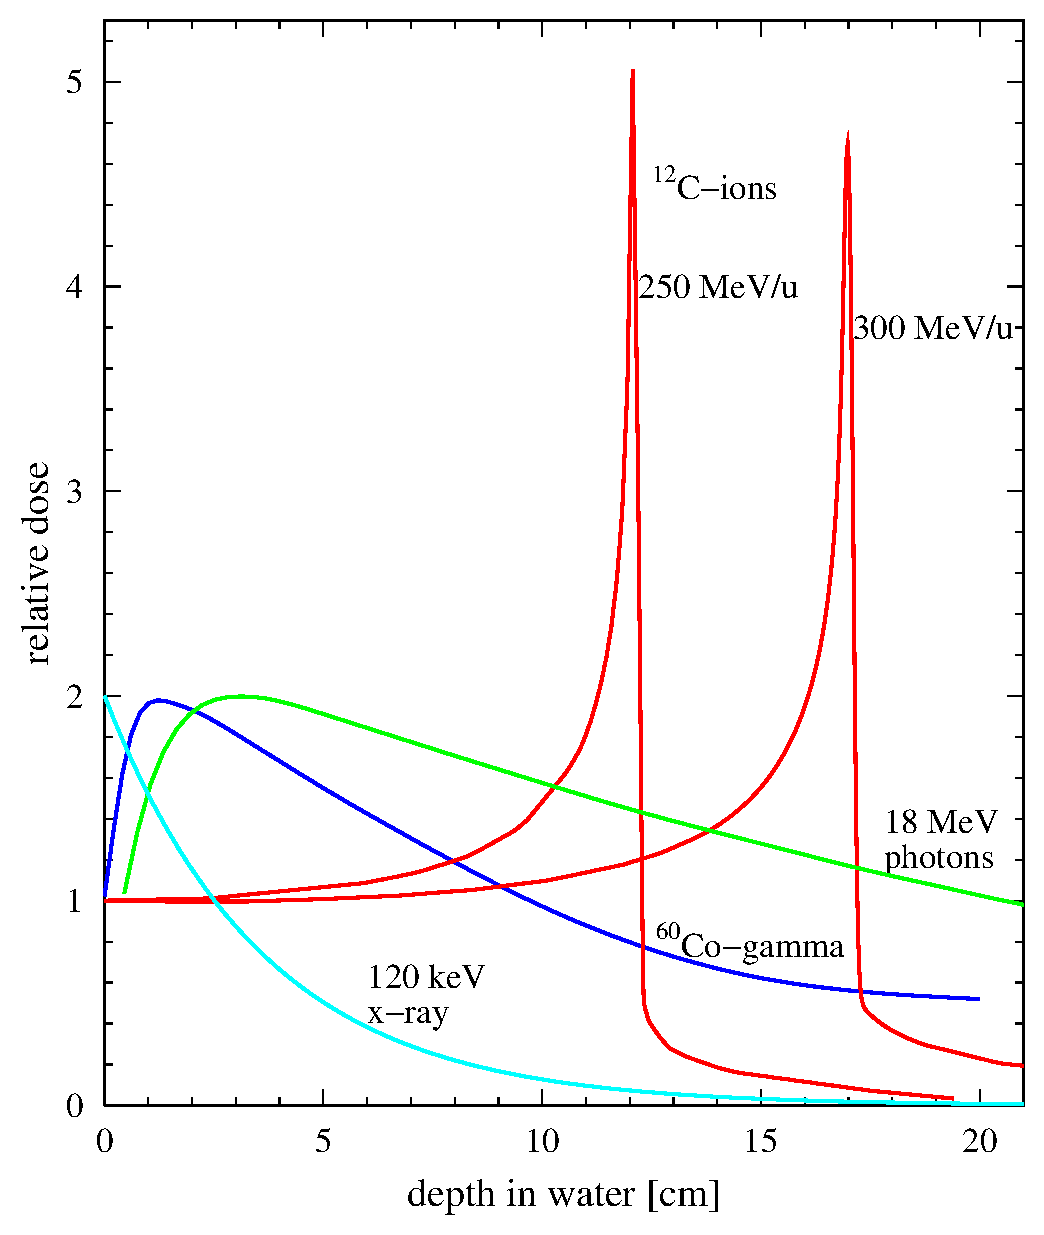
\includegraphics[scale=1]{depthdose.eps}
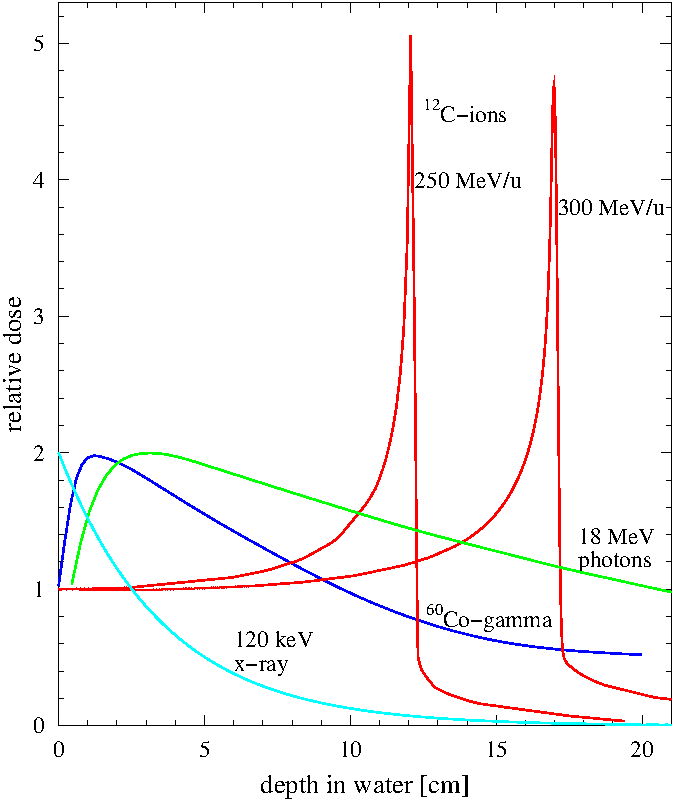
\includegraphics[width=0.9\textwidth]{./Fundamentals/Images/depthdose.png}
\caption{Photon and carbon ions depth dose distributions at different energies. Photons start with a build up, which is then followed by an exponential decrease. Ions deposit most of the dose at the end of the particle track - the Bragg peak. Figure taken from \cite{Schardt2010} }
\label{ddp}
\end{center}
\end{figure}

\subsubsection{Interaction of photons with matter}

Photons mostly interact with matter in one of the following ways: coherent or Rayleigh scattering, photoelectric effect, Compton scattering and pair production. The cross section $\sigma$, for each of these processes depends as well on the energy of the incident photons as on the atomic number of the absorbing material \cite{Lilley2006}. The decreasing photon intensity in matter, $I$, can be described as:

\begin{equation}
 I = I_{0} \cdot e^{- N \sigma x} = I_{0} \cdot e^{-\mu x}
 \label{expdecrease}
\end{equation} 

where $I_{0}$ stands for the initial intensity of the photons, $x$ the depth of the material in units of length, $N$ the atomic density of the material and $\mu$ the attenuation coefficient. The cross section, $\sigma$ is the sum of all possible Interaction processes:

\begin{equation}
{\sigma} = \sigma_{rayleigh} + \sigma_{photoelectric} + Z\sigma_{compton} + \sigma_{pairproduction} 
\end{equation}
The energy range of photons used in radiotherapy is between 100 keV and 25 MeV. The dominating process in this energy range is Compton scattering \cite{Alpen1998}.
The electrons resulting from Compton interaction scatter mostly in a forward direction. Therefore a maximum of the depth-dose profile occurs when electrons stop at a certain depth, 
the mean electron range. After this build up the dose deposition decreases exponentially (see Fig.~\ref{ddp} and Equation \ref{expdecrease}).

\subsubsection{Interaction of ions with matter}
\label{iion}
Ions can interact with matter either with elastic Coloumb scattering from target nuclei (nuclear stopping) or with inelastic collision with target electrons (electronic stopping).
At the ion energies used in radiotherapy, which are less then 500$\mathrm{MeV}/\mathrm{u}$, the electronic stopping is the dominating interaction. The result is ionization and excitation of the target atoms.

The mean rate of the ions energy loss in matter is described by the Bethe-Bloch formula \cite{Bethe1930, Bloch1933}. Since we are interested in low ion energies, a non-relativistic approximation ca be made:

\begin{equation}
- \left \langle \frac{dE}{dx} \right \rangle = \frac{ 4 \pi N_{e} z_{eff}^{2} }{ m_{e} v^{2} } \left( \frac{e^{2}}{4\pi \epsilon_{0}} \right) ^{2} \left[ln \left( \frac{2m_{e}v^{2}}{I} \right)+correction \right]
 \label{bethe}
\end{equation}



here $N_{e}$ is the material's electron density, $e$ and $m_{e}$ are the charge and mass 
of an electron, $\epsilon_{0}$ the electrical field constant and $I$ the mean excitation energy of the absorber material. 
Barkas formula \cite{Barkas1963} can be used for the approximation of the effective projectile charge $z_{eff}$: 

% \vspace*{-0.8cm}
\begin{equation}
 z_{eff} = z \left( 1 - e^{-125 \beta z^{\frac{2}{3}}} \right)
\end{equation}

where $\beta$ is the projectile speed in units of $c$.

The energy loss of the ions is proportional to $z_{eff}$ and inversely proportional to $v^2$. The shape of the curve in Fig.~\ref{ddp} can be explained as following: Ions enter the matter with a high velocity, resulting in a small energy deposition. Their velocity gradually decreases, which in turn increases the energy deposition. The maximum of the energy loss occurs right when the ions stop and it is called Bragg peak.

\subsubsection{Lateral scattering and range straggling of ions}
\label{scat}
As mentioned ions interact with matter mostly via electronic stopping at energies used in radiotherapy. However, nuclear stopping still occurs and it is the main reason for lateral scattering.
The angular spread of ions is dependent on the mass of the target nuclei and on the momentum of the incident ions \cite{Moliere1948}. The lateral scattering is proportional to the mass of the target nuclei and inversely proportional
to the momentum of incident ions. Carbon ions have thus less lateral scattering then protons. Experiments have shown that carbon ions have three times smaller angular spread compared to protons at the same range in water 
(15.6 cm, 150 MeV/u protons and 285 MeV/u $^{12}$C ions) \cite{Schardt2010}.

Statistical fluctuations of specific electronic stopping events cause range straggling of ions. If the number of collisions is high or the material is thick enough these fluctuations can be approximated by
a Gaussian probability distribution \cite{Bohr1940, Ahlen1980}. The straggling width $\sigma_R$ is proportional to:

\begin{equation}
 \sigma_R \propto R/\sqrt{M}
\end{equation}

where $R$ is the mean range of ions and $M$ the ion mass. Thus, the heavier the ion is, the less range straggling it has. Carbon ions have 3.5 smaller range straggling when compared to protons \cite{Schardt2010}.

\subsubsection{Nuclear fragmentation}
\label{nuclfrag}

When transversing through matter ions (except protons) can be fragmented into ions with lower atomic number. The lower Z fragments travel in the same direction as projectile ions and 
have a significant contribution to the deposited dose (see Fig.~\ref{iondd}). It is thus essential that fragments are included in the treatment planning, so that an accurate dose can be calculated.

After colliding with the target projectile fragments enter excited state. A de-excitation occurs through
emission of nucleons, nucleon clusters and photons. Two of the possible fragments of projectile $^{12}$C ions are isotopes $^{11}C$ and $^{10}C$, which are both $\beta^+$ emitters \cite{Kraft2000}.
The resulting positron is annihilated with electrons in matter, creating two photons, which travel in opposite direction. PET (Positron Emission Tomography) can take advantage of the process without exposing patient to additional radiation.

\begin{figure}[H]
\begin{center}
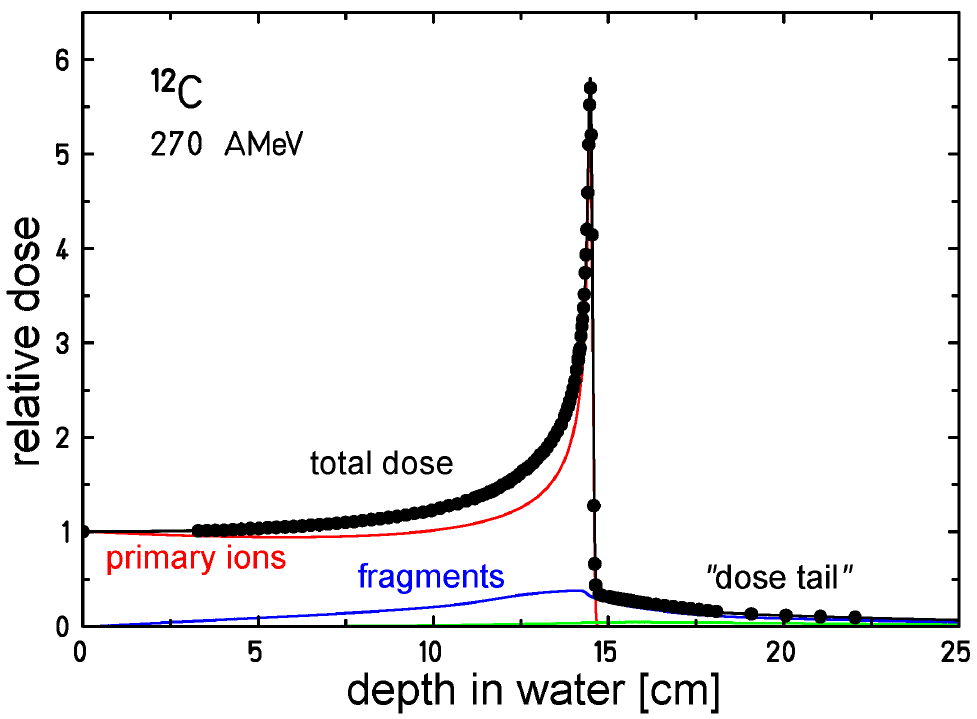
\includegraphics[width=0.7\textwidth]{./Fundamentals/Images/iondepthdosesum.png}
\caption{Impact of fragmentation on a depth dose distribution of carbon ions. Main contribution to the overall deposited dose (black line) comes from the primary ions (red line). The produced fragments 
(blue line) have a smaller impact, but non-negligible. The most profound effect is seen in the dose tail behind the Bragg peak, where dose comes only from fragments. Figure taken from \cite{Groezinger2004}}
\label{iondd}
\end{center}
\end{figure}

\subsubsection{Secondary electrons and track structure}

Ions used in radiotherapy loose most of their energy via inelastic Coulomb scattering on target electrons. Electrons liberated from target by ions are called secondary electrons or $\delta$-electrons. 
$\delta$-electrons travel through matter, scatter further and may produce secondary ionization of the target atoms. When $\delta$-electrons energies are larger than $>$50 eV,
ionization becomes the dominant process, which produces a large number of additional electrons \cite{Kraft2000,Schardt2010}.

The radial dose profile and track diameter is defined by the energy spectrum of the $\delta$-electrons. Most of the $\delta$-electrons are concentrated around the projectile ions path, since they receive small energy transfers 
or are scattered in the direction of incident ions. Different models \cite{Chatterjee1976,Katz1999} and Monte Carlo simulations \cite{Paretzke1986,Kraemer1995} predict radial dose fall-off approximately with $1/r^2$ for radial distance $r$. Varma et. al. have confirmed 
this experimentally \cite{Varma1977}. The maximum radial distance $r_{max}$ is defined by the most energetic $\delta$-electrons, which are related to energy, $E$, of the projectile ions \cite{Kiefer1986}.

\begin{equation}
 r_{max} = E^{1.7}
\end{equation}

Following equation \ref{bethe}, $E$ is correlated to $Z^2$ and $1/\beta^2$, meaning that track structure is highly dependent on the projectile ion species and energy as demonstrated in Fig.~\ref{track}:
Carbon ions have much more dense ionization structure compared to protons \cite{Kraemer2010}. $\delta$-electrons have low energies, and thus the $r$ is on nanometer scale. As the energy of projectile ions decreases, their
stopping power increases and causes significantly larger number of $\delta$-electrons. The energy deposited by $\delta$-electrons in medium is described using the Linear Energy Transfer (LET), which is closely related to 
$dE/dx$. Fast ions, with little ionization, have thus small LET, while slow ions, with large ionization, have a high LET.


\subsection{Radiobiology}

Ionizing radiation (photons and ions) causes damage throughout the cell. However the most susceptible part to radiation is the
carrier of genetic information, the deoxyribonucleic acid (DNA), located in the cell nucleus \cite{Munro1970}. Radiation can damage DNA directly or indirectly.

Ionization and consequent destruction of DNA molecular bonds via radiation is a direct effect (see Fig.~\ref{ida}b) and is typical for high-LET radiation. On the other hand, an indirect effect is when radiation hydrolysis water around DNA and produce highly reactive hydroxyl-radicals, OH 
(see Fig.~\ref{ida}a). Even though OH radicals decay fast, they are still able to cause severe damage to DNA. The formation of OH is typical for low-LET radiation like photons. The two processes, direct and indirect, are not exclusive and can damage DNA in parallel.


\newpage

\begin{figure}[H]
\begin{center}
% 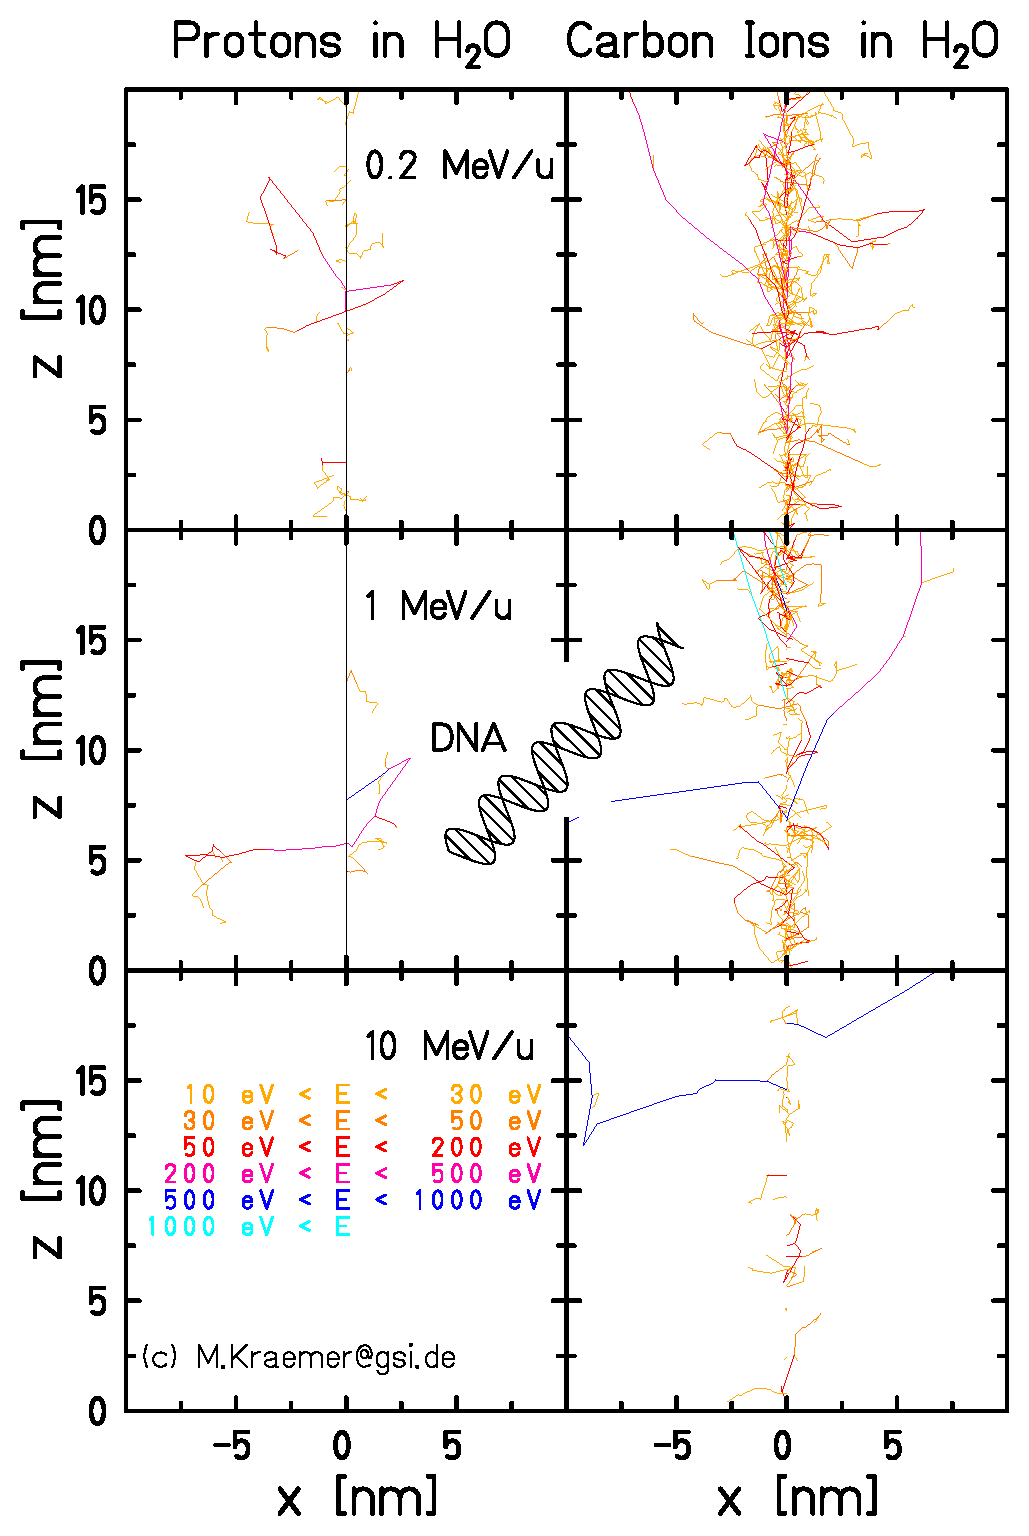
\includegraphics[scale=0.75]{trackstructure.eps}
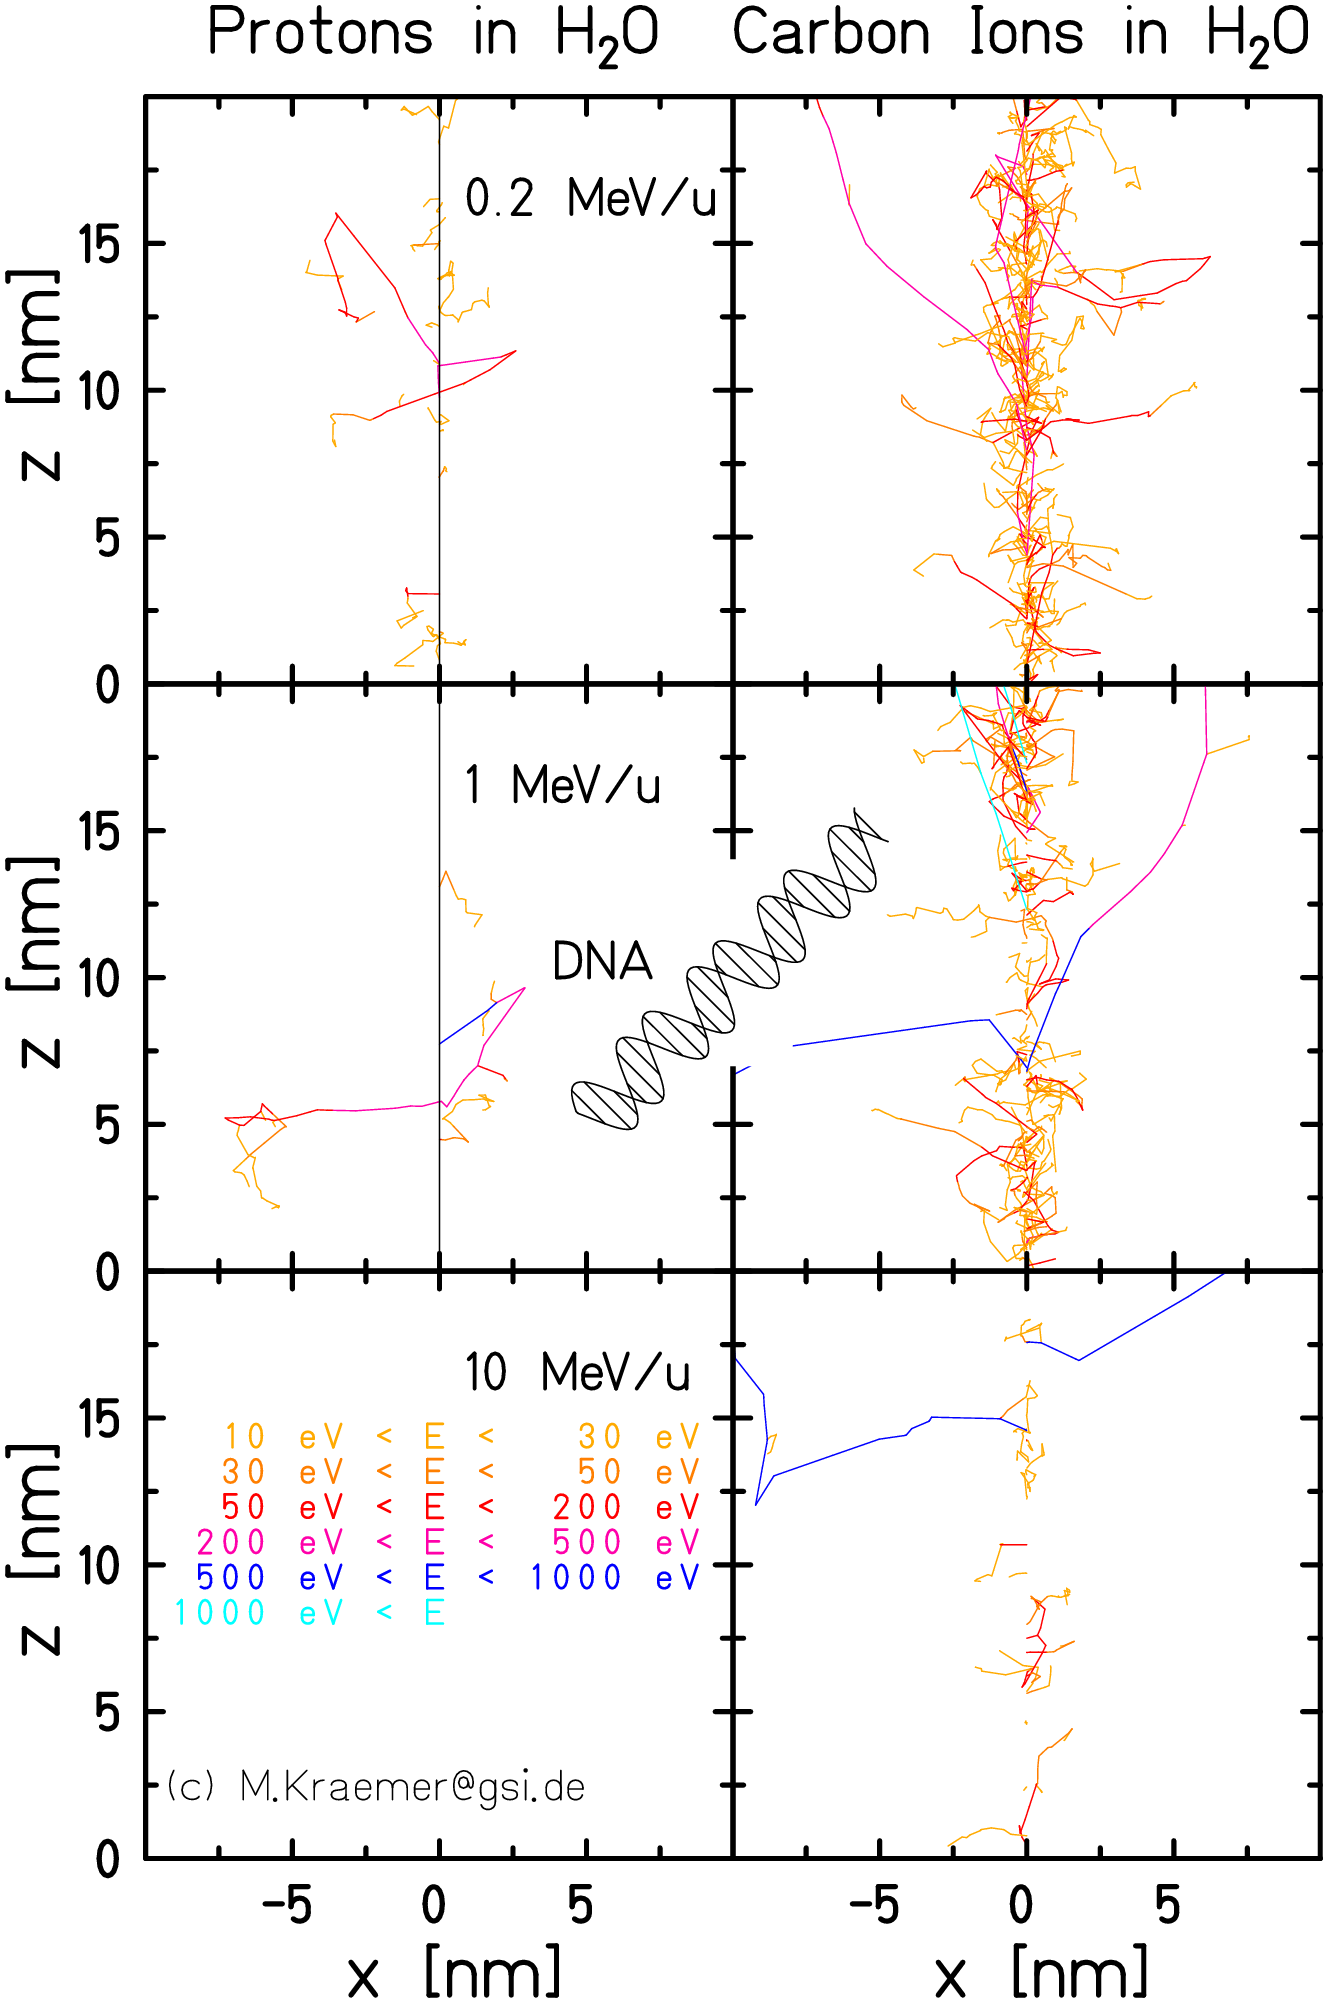
\includegraphics[width=0.8\textwidth]{./Fundamentals/Images/trackstructure.png}
\caption{Track structure of ions in water at different energies. The distribution of $\delta$-electrons is highly dependent on ion species and their energy.
A molecule of DNA is displayed for size comparison. Figure courtesy of Michael Kr\"amer.}
\label{track}
\end{center}
\end{figure}


\begin{figure}[H]
\begin{center}
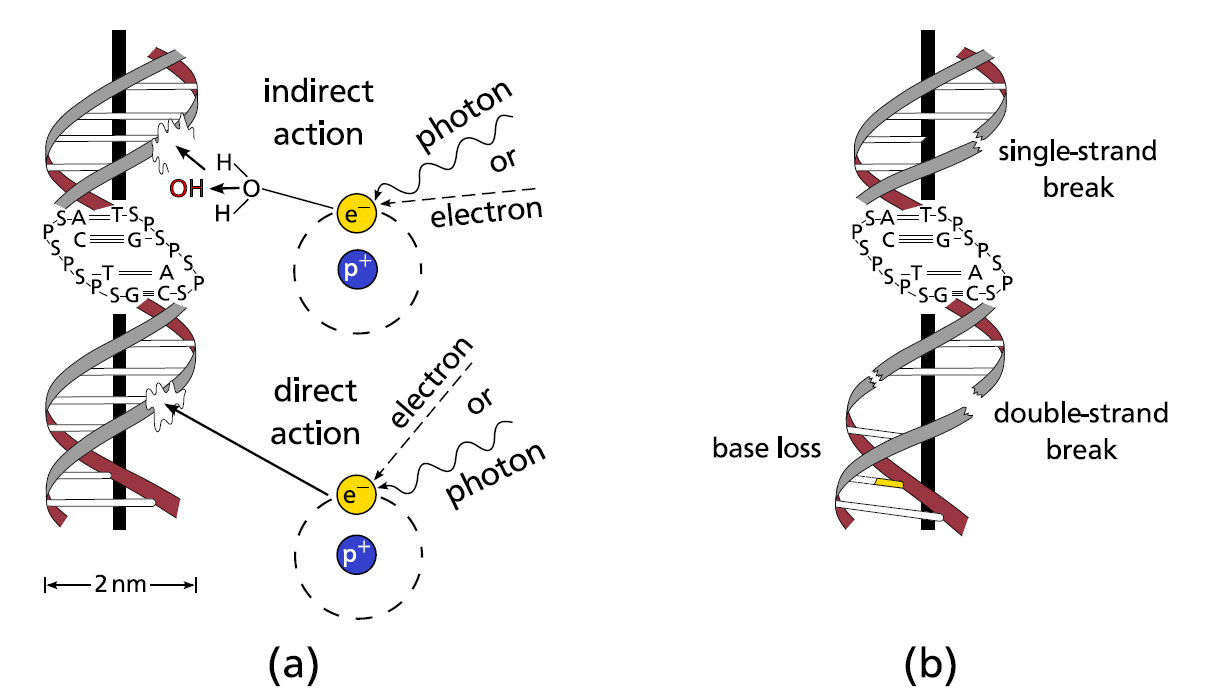
\includegraphics[width=0.9\textwidth]{./Fundamentals/Images/SSB_DSB.png}
\caption{Types of DNA damage caused by radiation (a) Indirect damage occurs, when radiation forms free radicals hydroxyl radicals (OH), which can damage DNA. (b) Direct effects of radiation can cause single or double-strand breaks. 
Figure taken from \cite{Richter2012}}
\label{ida}
\end{center}
\end{figure}


Damage to DNA can result in either single strand breaks (SSB) or double strand breaks (DSB) as shown in Fig.~\ref{ida}b). When one of the double strands in the DNA helix is destroyed (SSB), it can usually be easily repaired by cell 
repair-mechanisms, since the complementary base is intact. If the bases on both stands are destroyed (DSB) the DNA damage is much more complex and can lead to the breakage of the chromatin. The cell repair-mechanisms can handle DSB as well, 
albeit not as efficient as SSB. However if there are clustered DSBs, the damage is usually too severe for repair-mechanisms to undo it. The changes in damaged DNA can lead to carcinogenesis or cell death. The aim of radiotherapy is to 
cause an apoptosis - a controlled self-inactivation of the cell due to the DNA damage. Beside apoptosis, cell can also undergo necrosis, an uncontrolled cell death. Cell necrosis often causes response from the immune system, leading to inflammation, which
radiotherapy strives to avoid. DNA can also be damaged to such extent, that cell cannot proliferate indefinitely - a effect known as clonogenic cell death.


\subsubsection{Relative Biological Effectiveness}
\label{RBE}

Fig.~\ref{track} shows the size of DNA molecule in comparison with proton and carbon ion distribution of $\delta$-electrons around their track. 
A clustered DSB occurs preferably around Bragg peak due to large ionization densities. Less cells will survive a clustered DSB, compared to DSB or SSB. Ions have large ionization density and is one of the main advantages over photons in the radiotherapeutic sense. Since most of the clinical experience about
cell response to radiation comes from photons, the biological effect of ions is usually described relative to a reference photon response. Relative biological effectiveness (RBE) is therefore defined as the ratio of the reference 
photon dose to the dose level of a specific ion radiation at the same biological effect (isoeffect):

\begin{equation}
 RBE = \left.\frac{D^{ref}_{photon}}{D_{ion}} \right|_{isoeffect}
\end{equation}

It is important to note at this point that RBE values are valid only for the same effect - the same biological endpoint and the same reference radiation. The most interesting biological endpoints in radiotherapy are cell survival and
side effects. RBE values are usually obtained from cell survival curves (see Fig.~\ref{dosedep}). Cell survival curves, S, are commonly modeled by an exponential linear-quadratic (LQ) model \cite{Fowler1989}:

\begin{equation}
 S(D) = e^{-\alpha D - \beta D^2}
 \label{lq}
\end{equation}

$\alpha$ is a coefficient related to a single event cell killing and $\beta$ coefficient related to a double event cell killing. The ratio of $\alpha / \beta$ is a characteristic of the cell type, namely the tissue 
capacity to repair radiation damage. A small $\alpha / \beta$ ratio means cell is radioresistive (high repair capacity) and vice versa.
As seen in Fig.~\ref{dosedep} and Eq. \ref{lq}, RBE values are dependent on the dose level. Hence in ion radiotherapy, beside the physical absorbed dose, a photo-equivalent or biological dose incorporating the RBE also plays an important role. 
The unit for biological dose is Gy (RBE) \cite{ICRU2007}. 

Besides a dose level, RBE also depends on the LET, the particle species and the tissue type \cite{Kraft2000}. Therefore RBE modeling is a complex topic.
At GSI, RBE is calculated using the \textit{local effect model} (LEM) developed by Scholz et al. \cite{Scholz1994}. There are two main assumptions in the LEM model. First is that localized biological 
effects are independent on the radiation type. Second assumption is that the photon response is the same for all dose levels (high and low).
The difference between different radiation types comes from the dose deposition in a small volume in the cell nucleus.
At the same total dose, many photons create a homogeneous dose distribution over a cell nucleus, while few ions cause a highly localized dose distribution around their track.

\newpage

\begin{figure}[H]
\begin{center}
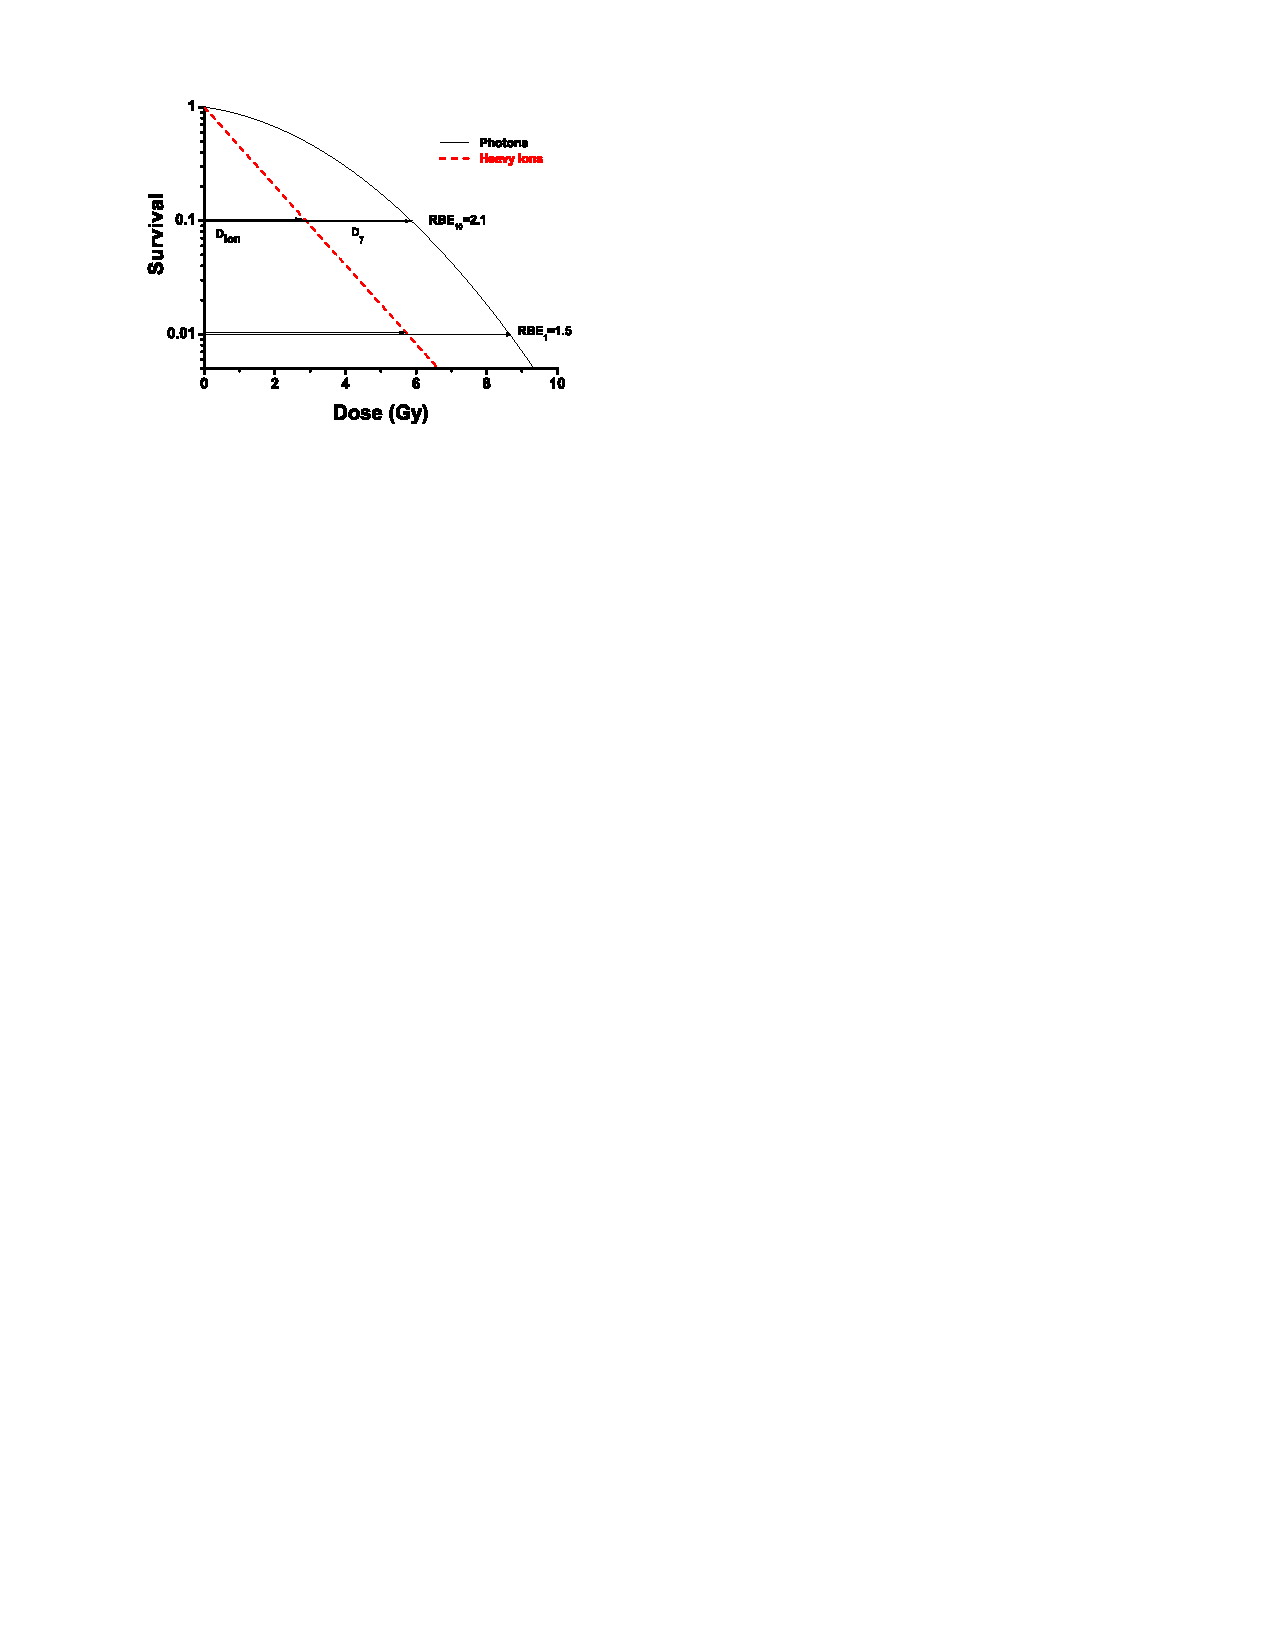
\includegraphics[width=0.6\textwidth]{./Fundamentals/Images/dose_dependence.pdf}
\caption{Typical cell survival curve for photons (black solid line) and heavy ions (red dashed line). Photon line shows typical shouldered form, described by linear-quadratic model.
Heavy ions show a much steeper decrease with dose. The RBE value can be calculated by looking at the points at the same survival value - same biological effect. Figure taken from \cite{Schardt2010}}
\label{dosedep}
\end{center}
\end{figure}

 
LEM can thus predict dose response, by comparing
photon response at the high local dose level. LEM was used clinically as well in GSI pilot project from 1998 - 2007 \cite{Kraemer2000, Kraemer2000a} as in HIT since 2009. LEM has received several revisions \cite{Elsaesser2006, Elsaesser2007, Elsaesser2009} and experimental verifications
\cite{Mitaroff1998, Kraemer2000a, Kraemer2003}. 

RBE for carbon ions ranges from 1 in the entrance channel, to a value around 5 at 
the Bragg peak \cite{Kraft2000}. The highest RBE for carbon ions is right around Bragg peak, which gives carbon ions a great advantage, since there is an increased 
biological effectiveness at target tissue compared to the normal tissue in the entrance channel. In proton therapy a constant RBE value of 1.1 across the treatment field
is used \cite{Paganetti2002}.

\subsubsection{Fractionation}

Radiotherapy applies a basic principle of radiobiology that dose fractionation spares all cell types. For a given total dose
more cells will survive with dose delivered across multiple fractions, compared to a single dose, because cells will have time to repair
radiation induced sub-lethal damage between fractions.
With dose $d$ delivered over $n$ fractions, equation~\ref{lq} can be rewritten as \cite{Shrieve2011}

\begin{equation}
 S = (e^{-\alpha d - \beta d^2})^n
\end{equation}

The biologically effective dose (BED) is defined as:

\begin{equation}
 BED(Gy_{\alpha/\beta})=nd\left[1 + \frac{d}{\alpha/\beta} \right]
\end{equation}

with the total dose $D$ equal to $n \times d$, we can define fractionation factor $F$ as

\begin{equation}
 F = \left[1 + \frac{d}{\alpha / \beta} \right]
\end{equation}

so that BED = $D \times F$. $F$ increases with $d$, but decreases with $\alpha / \beta$. Lower $\alpha / \beta$ (late-responding tissue)
means higher $F$ and a higher $\alpha / \beta$ (early responding tissue) moves $F$ towards 1.


\subsubsection{Hypo-fractionation}

In recent years hypo-fractionation has showed promising results over wide range of tumors \cite{Yamada2008, Greco2011, Halasz2013}. 
Hypo-fractionation consists of 1-3 fractions of very high doses, up to 24 Gy in a single fraction (single-dose). The theory behind hypo-fractionation is still under research
and no consensus has yet been reached. On one hand, LQ model predicts higher BED for hypo-fractionation. On the other hand, Garcia-Barros et al. proposed additional mechanism at work \cite{Garcia2003}.
They presented a two target model, which suggest that tumor response to irradiation is defined not only by tumor cell type (as in LQ model) but also by micro-vascular
sensitivity. With excluding targeted enzymes from knock-out mice, they showed that tumors with reduced micro-vascular endothelial apoptosis grew 200-400 \% faster than a control group. The study, however, was challenged on several grounds and is controversal.
  

\subsection{Application technique}

The use of X-rays for treating patients has more than a century long history. There is a lot of research and practical knowledge regarding the clinical usage of X-rays. Particle therapy, on the other hand, is a more novel technique, with
more patients being treated every year. In the following sections an overview will be given of how the irradiation is actually delivered to the patient for both modalities with the emphasis on ion therapy.

\subsubsection{Photon therapy}

In photon therapy high energy x-rays (MV) are used for tumor irradiation. X-rays are produced in a linear accelerator (LINAC). Electrons are accelerated with energies from 2-25 MeV and collided with a high-density target (tungsten), where
x-rays are produced via bremsstrahlung. The beam is then directed to the patient and conformed to the tumor shape. The beam is shaped either by blocks at the head of the machine or by a multileaf collimator. A multileaf collimator is made of
individual leaves, that can be moved to represent the tumor's shape in the beam's eye view, see Fig.~\ref{MLC}.

Linear accelerators are usually placed on a gantry, which can be rotated around the patient. This allows beams to enter the patient from any angle. 
The arbitrary choice of beam angle is used in a 3-dimensional conformal radiotherapy, where a variable number of beams is used. 
Each beam is then shaped with a multileaf collimator. Even more precise technique is intensity-modulated radiotherapy (IMRT). IMRT allows treating complex tumor shapes, e.g. when the tumor is in proximity of a critical structure.
Volumetric modulatec arc therapy (VMAT) uses continuous irradiation together with continous gantry rotation and multileaf collimator shaping. VMAT is able to produce even more conformal dose shapes than IMRT.

\subsubsection{Ion therapy}

In order for ion therapy be successful, ions must be accelerated to appropriate energies (several hundred MeV/u), the beam must be transported to target area and guided
onto the target with the required accuracy.

\newpage

\begin{figure}[H]
\begin{center}
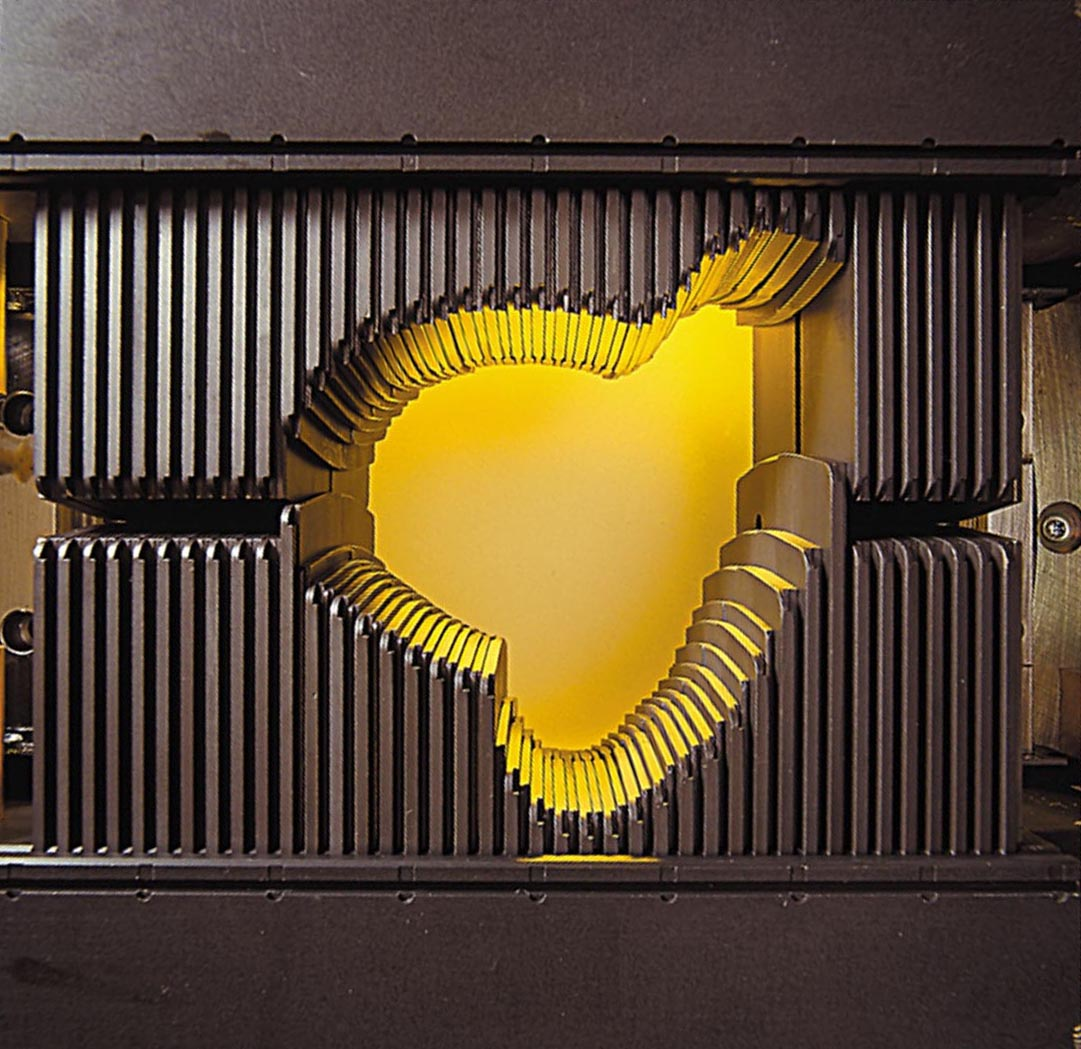
\includegraphics[width=0.7\textwidth]{./Fundamentals/Images/MLC.png}
\caption{A schematic picture of a multileaf collimator. Individual leaves (marked with numbers) are positioned so that exit beam from linear accelerator conforms to the patient tumor in a beam's eye view. Picture taken from \cite{MLC}.}
\label{MLC}
\end{center}
\end{figure}

% \begin{figure}[H]
% \begin{center}
% 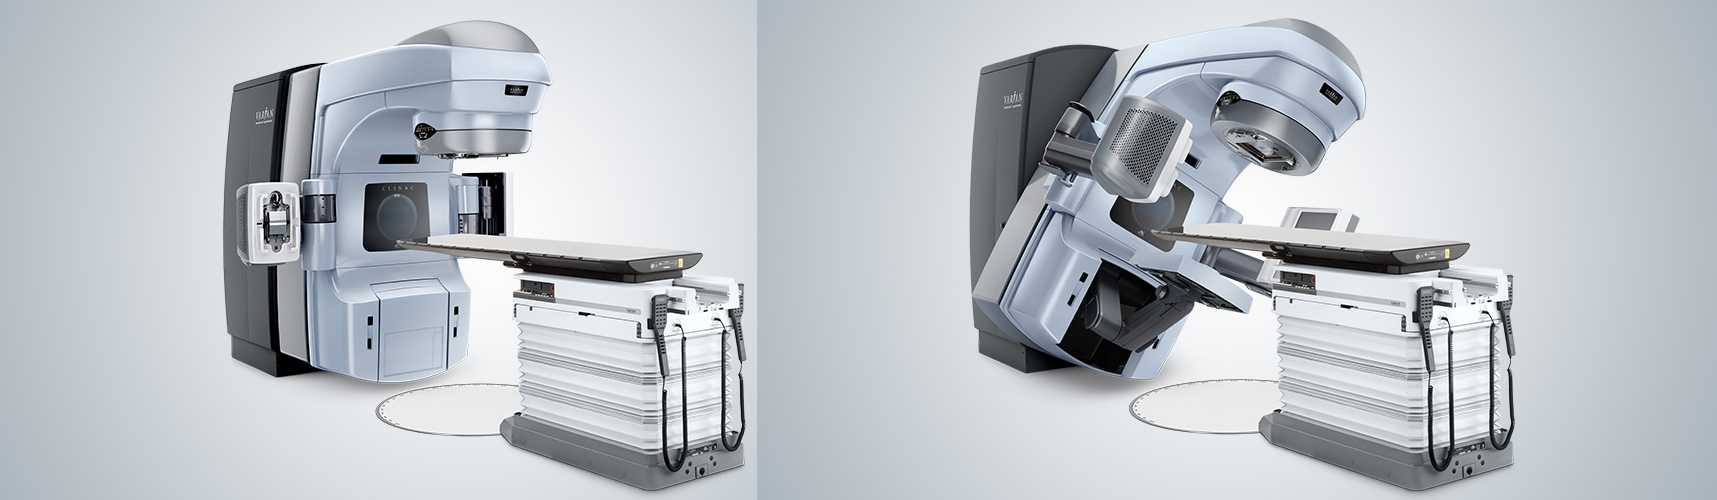
\includegraphics[width=0.9\textwidth]{./Fundamentals/Images/gantry.png}
% \caption{A picture of a modern photon delivery system with gantry at two angles. Gantry can rotate 360 degrees around the patient. Picture taken from \cite{MLC}.}
% \label{gantry}
% \end{center}
% \end{figure}




Ion are accelerated either with cyclotrons or synchrotrons accelerators. \textbf{Cyclotrons} can be built in a compact design and offer a continuous beam with
stable intensities. Cyclotrons and only be used for protons and particle energies can not be regulated and therefore passive energy degraders are needed. Active energy variation is possible with \textbf{synchrotrons}, where a linear
accelerator is used to inject ions into the synchrotron and then the beam is regulated with ion optics. Synchrotrons are used in all heavy ion therapy centers, while cyclotrons are most
commonly used for proton therapy.

Each tumor has a unique shape, size and position in patient. Therefore a single Bragg peak would not provide adequate dose and a beam has to be properly shaped. Two beam shaping systems
are in use - passive and active beam shaping. In the next two sections both will be explained.


\subsubsection{Passive beam shaping}
\label{Sec::Passive}

The general idea of passive beam shaping is to transform a beam of a fixed single energy into the shape of the tumor. This is done in several steps as schematically shown in Fig. \ref{passive}. Firstly, the beam is broadened using a scattering device (passive double scattering systems or magnetic wobbler)
in order to obtain a broad, flat profile. In the next step, the beam is spread out over the required energy range with a range modulator. Usually a range modulator consist of rotating wheels of various thickness or a ridge filter \cite{Chu1993}. A beam of fixed energy is thus expanded into so-called \textit{spread-out Bragg peak (SOBP)}, which is moved to the required depth using a range shifter. The final two devices in beam's path are built for each patient individually. Collimator shapes beam in a lateral direction, while compensator adjusts SOBP to the distal edge of the tumor. However, compensator cannot adjust dose in the proxima ledge of the tumor, resulting in an access dose to the healthy tissue (hatched area in Fig. \ref{passive}).
 
Passive beam shaping offers more robust and faster treatment delivery in contrast to active beam shaping. However, it lacks tumor conformity, the dose cannot be modulated and each patient needs individually tailored devices for each beam used in the treatment.
 Furthermore, the beam travels through some material, exposing patient to additional dose due to fragmentation.

 \newpage
 
\begin{figure}[H]
\begin{center}
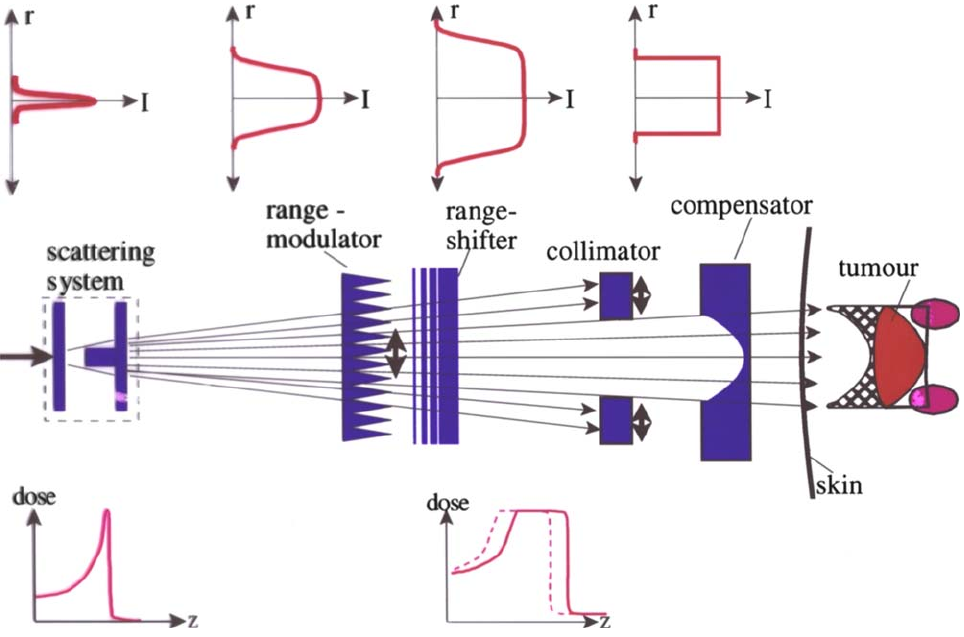
\includegraphics[width=0.7\textwidth]{./Fundamentals/Images/deliverypassive.png}
\caption{Schematic presentation of a passive beam shaping. A scattering system is used to broaden the beam. Afterwards a range modulator spreads out Bragg Peak to the required energy range.
The spread out Bragg peak is then shifted to a specific energy with a range modulator. Finally, patient specific collimator and conformator serve for lateral and longitudinal conformity, respectively.
The proximal edge of the tumor cannot be shaped, as shown with hatched area. Figure taken from \cite{Schardt2010}.}
\label{passive}
\end{center}
\end{figure}

\subsubsection{Active beam shaping}
\label{Sec::Active}

In contrast to passive beam shaping, active beam shaping works by dividing tumor into small points, which are then irradiated using a thin pencil beam. Tumor is first segmented into iso-energy slices (IES) and each of IES
is covered with a 2 dimensional grid (raster points). A thin pencil beam is deflected from raster to raster point, irradiating each one with designated dose. The technique allows irradiation of arbitrary shape, without introducing any additional patient specific 
hardware. The lack of additional material in front of the patient also means less dose due to lesser neutron flux. Furthermore with the option to modulate dose in each point, dose in tumor is very conformal with less dose to healthy tissue.

There are differences in specifics of active beam shaping and the GSI system of three-dimensional scanning system will be given here \cite{Haberer1993,Kraft2000,Schardt2010} and a schematic presentation is shown in Fig.~\ref{scanning} and Fig.~\ref{active}.
A synchrotron provides a thin pencil beam of $^{12}$C ions with a variable energy in the range of 30 - 400 MeV/u. The energy defines the position of the Bragg peak in depth. Fig. \ref{active}b shows how the Bragg peaks are stacked in depth to cover longitudinal extension of the tumor.
The thin pencil is guided by two magnetic deflection units to irradiate each raster point. The specific dose in each raster point is calculated in the treatment planing.
During treatment the beam stays on each raster point until intensity monitoring system measures the designated dose. Then it is moved to the next raster point. When the whole IES is irradiated, the treatment waits for the next IES comes from accelerator.

Fig.~\ref{active}a displays how dose homogeneity in the target is achieved. To achieve flat dose distribution with Gaussian beam profile, beam's full width half maximum is three times the lateral raster spacing. Such configuration offers robustness for uncertainties of the beam spots.
The spacing between individual IES is usually 3 mm, providing enough overlap between individual Bragg peaks. However, the number of IES should be kept low, since the changing of the beam energy takes most of the time and hence prolongs the treatment. Instead of using high number of
 IES, Bragg peaks are broadened in longitudinal direction by a using ripple filter (RiFi) - a device similar to ridge filters used in passive beam shaping. 

\subsection{Motion in radiotherapy}
\label{sec:motion}

Patient motion can have a profound effect on the radiotherapy. It can cause large deviations from the planned dose, resulting in under- or over-dosage in target and excess dose in OAR. Motion types, its extent and origin is therefore a vast topic of research. 
A brief introduction will be given here, for an in-depth explanation reader is pointed to review by Langen and Jones \cite{Langen2001}.

\newpage

\vspace*{0.6cm}

\begin{figure}[H]
\begin{center}
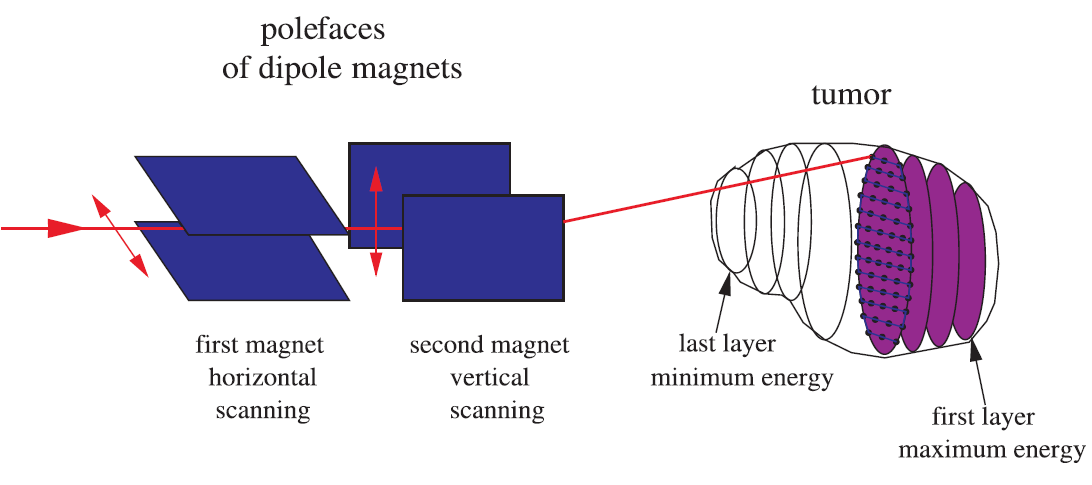
\includegraphics[width=0.9\textwidth]{./Fundamentals/Images/therapy.png}
\caption{Schematics of GSI's active beam shaping. Tumor is divided into isoenergy slices, which are further overlayed with a 2 dimensional grid. 
Longitudinal direction (in beam's eye view) is varied with particle energy from accelerator, while lateral is via a magnetic scanning system. Figure taken from \cite{Kraemer2009}}
\label{scanning}
\end{center}
\end{figure}


\begin{figure}[H]
\begin{center}
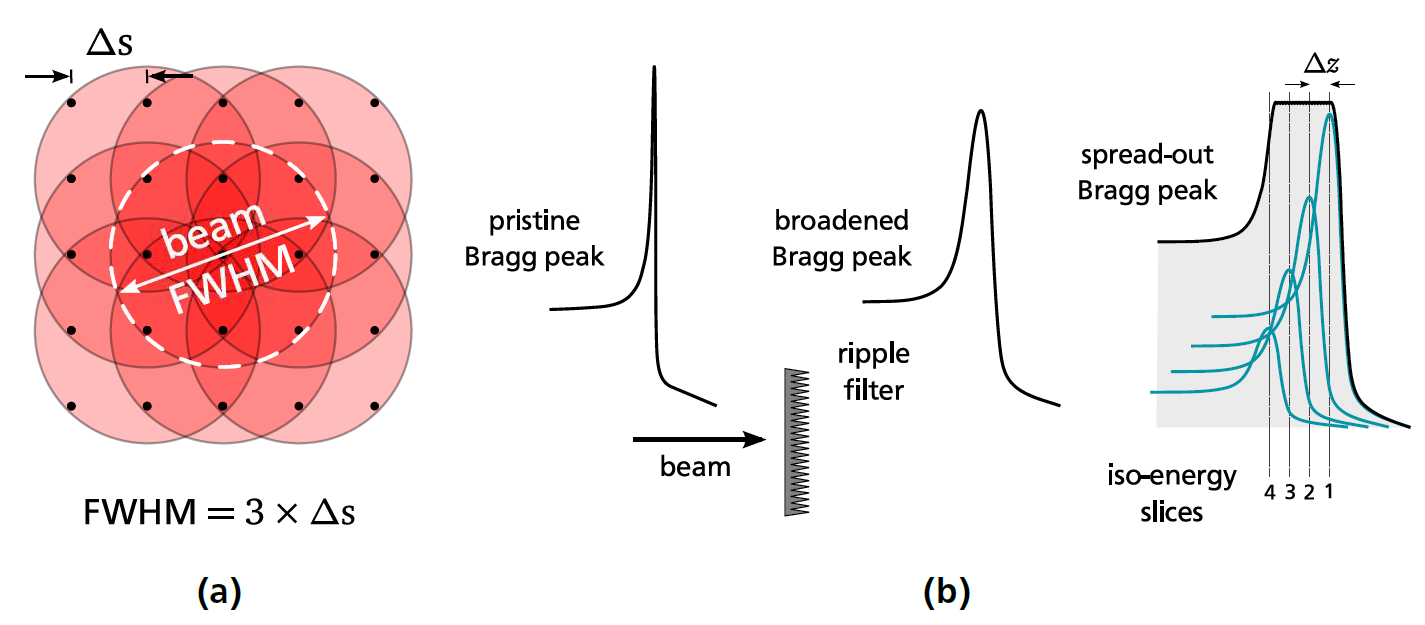
\includegraphics[width=0.9\textwidth]{./Fundamentals/Images/active.png}
\caption{Schematic presentation of how target dose homogeneity is achieved in active beam shaping. a) To provide sufficient homogeneity in lateral direction (in beam's eye view) full width
half maximum of beam is three times the spacing between raster points. b) Bragg peaks are broadened in depth with a ripple filter and then stack to provide longitudinal dose homogeneity. 
Figure taken from \cite{Richter2012}}
\label{active}
\end{center}
\end{figure}


\newpage




\subsubsection{Motion types}

There are three main types of motion: patient positioning, inter- and intra-fractional motion. All three motion types are shown in Fig. \ref{motion}.
\newline
\textbf{Patient motion} is difference in patient position between image acquisition (e.g. CT) used for treatment planning and actual delivery. Patient motion introduces changes in tumor shape and tumor position. To overcome patient 
position uncertainties, patient immobilization and dedicated protocols are used.
\newline
\textbf{Interfractional motion} happens between two treatment sessions (fractions) and results in anatomical changes in a patient. It occurs on a time scale of hours and days. For lung cancer patients, tumor shrinks and lung density can change between fractions \cite{Mori2009}. 
Also changes in breathing pattern can impact treatment delivery. Additionally, the tumor baseline drifts significantly \cite{Sonke2008}. Repeated imaging and replanning reduces the impact of the interfractional motion, but requires additional time.
\newline
\textbf{Intrafractional motion} is mainly caused by respiration and heart beat, but also peristalsis. The time scale ranges from seconds to minutes. In this thesis we investigated treatment of lung cancer, so focus lies on respiratory motion. Respiratory motion varies from patient to patient and 
it is responsible for tumor motion from a mm range to a couple of cm \cite{Shirato2004a}. Tumor size and T-staging are also correlated to tumor motion \cite{Liu2007}. The respiratory-induced motion is largest in superior-inferior (SI) direction rather than 
in the anterior-posterior (AP) or left-right (LR) directions \cite{Seppenwoolde2002, Britton2007, Liu2007}.

\newpage

\begin{figure}[H]
\begin{center}
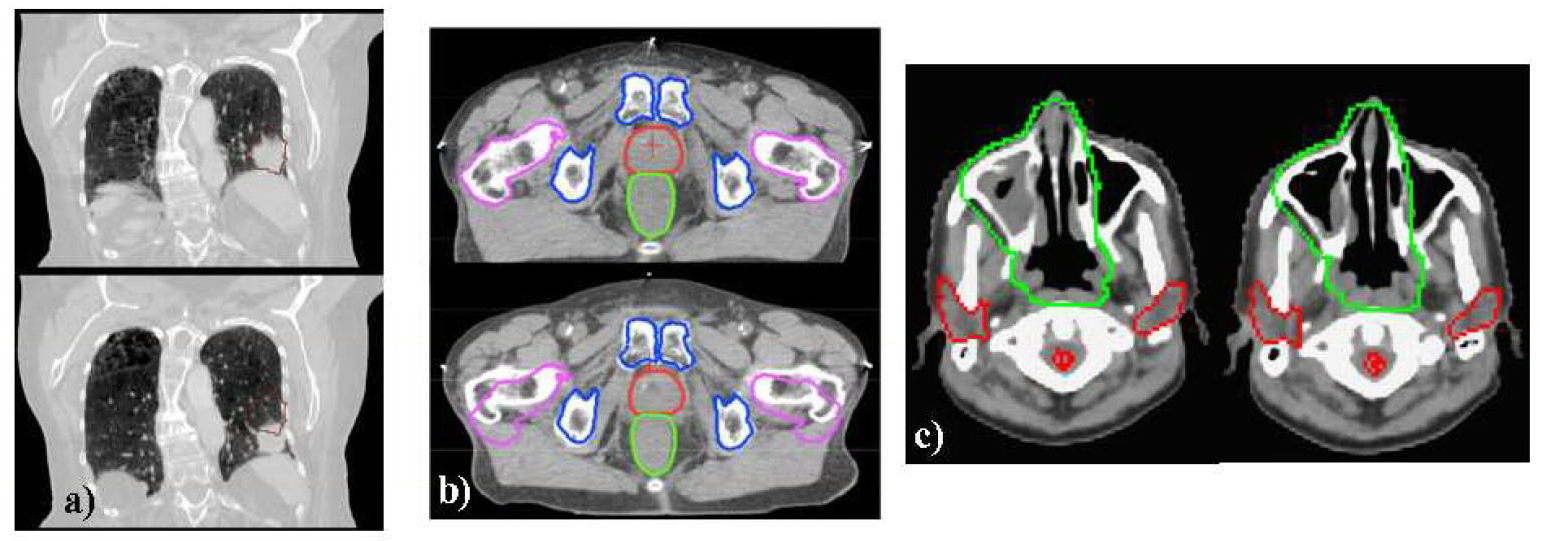
\includegraphics[width=0.9\textwidth]{./Fundamentals/Images/motion_examples.png}
\caption{Examples of the three major motion categories. On the left side (a) a lung tumor is displayed, which moves due to the respiration 
of the patient (intrafractional motion). Interfractional position changes are exemplary shown in the middle (b), where two CT scans of a 
prostate patient are compared. Density variations between two CT scans are shown in (c). Figure taken from \cite{Engelsman2011}}
\label{motion}
\end{center}
\end{figure}

\subsubsection{Motion mitigation techniques}

While all three motion types have to be addressed in treatment planning, special focus will be given on intrafractional motion mitigation. Photon radiotherapy or particle radiotherapy with passive beam shaping 
use larger safety margins to encompass the whole tumor motion as explained in Section~\ref{treatmentPlanning}. However, larger safety margins are not enough to mitigate motion when active beam shaping is used. The beam delivery 
sequence and target motion interfere with one another, resulting in over- and underdosages in patients. This effect is called interplay and it has been thoroughly reviewed elsewhere \cite{Phillips1992,Bert2008}. The effect of interplay depends
on many factors, such as motion amplitude, beam direction, starting breathing phase etc. Three main techniques are currently established to counteract interplay: rescanning, gating and beam tracking. Several others techniques exist
to reduce the effect of tumor motion, such as abdominal compression, jet ventilation, apneic oxygenation etc., but will not be described here, since the scope of this thesis is on free-breathing patients.


\textbf{Rescanning} is a technique that uses statistical averaging of different interplay patterns \cite{Phillips1992}. Instead of applying the whole dose $D$ at once, the target is scanned $N$ times, each
time irradiated with $\mathrm{D}/\mathrm{N}$. The result is a Gaussian dose distribution around $D$ with no interplay (static case), as shown in Fig. \ref{rescanning}. With more rescans (larger $N$), better dose homogeneity is achieved, because the variance is proportional
to $\mathrm{1}/\mathrm{N}$. Technically the method is the easiest to implement of the three mentioned, since no real-time motion monitoring is necessary. The treated volume must be enlarged to at least encompass target in all motions states (in
contrast to gating), which introduces additional dosage to normal tissue. Rescanning is currently used at NIRS, Tokyo (Japan) and at \textit{some proton centers}.
\newline
\begin{figure}[H]
\begin{center}
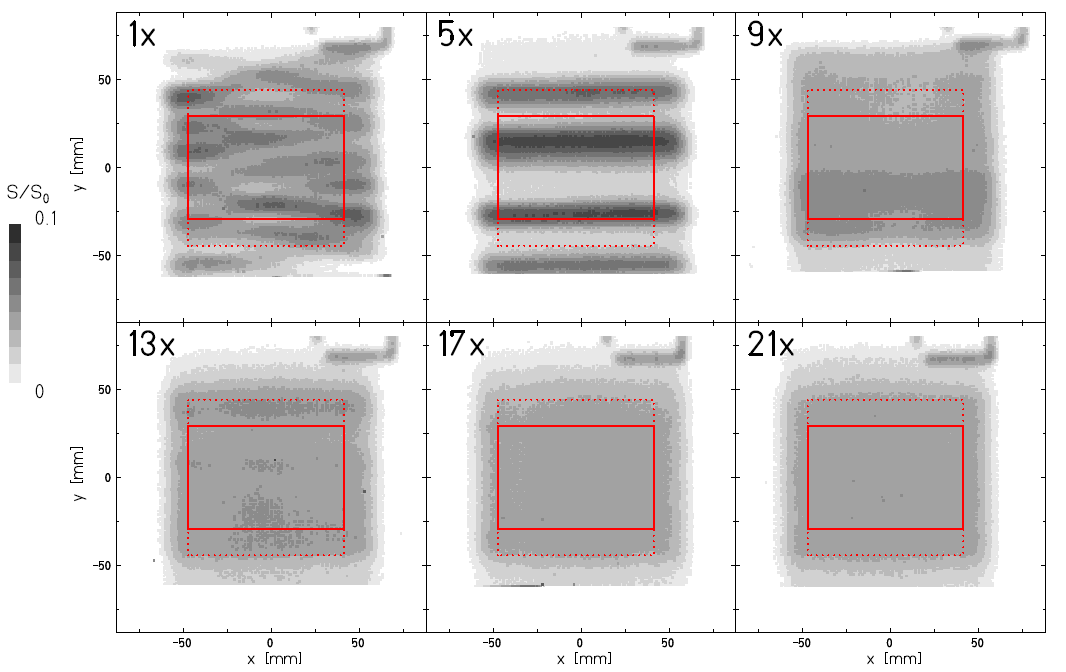
\includegraphics[width=0.7\textwidth]{./Fundamentals/Images/rescanning.png}
\caption{Film irradiation with rescanning. With statistical averaging of multiple interplay patterns dose in the target (solid red square) becomes homogeneous. Figure taken from \cite{Bert2009}.}
\label{rescanning}
\end{center}
\end{figure}

\textbf{Gating} applies irradiation only in a selected part of the breathing cycle in a so-called gating window (GW) \cite{Minohara2000,Lu2006}. Usually, the end-exhale position is used as the center of the GW, as highlighted in Fig.~\ref{gating}.
A motion monitoring signal is used to control beam extraction. While there is limited additional normal tissue irradiation, the treatment time is prolonged due to frequent beam interruptions as shown in Fig. \ref{gating}.
Conventional radiotherapy and passive beam shaping also employ gating to reduce the effects of motion on treatment delivery.
\newline
\textbf{Beam tracking} is a method where the tumor is followed by the beam throughout different motion phases in real time. Similar to gating, beam tracking is not limited to active beam shaping. It was even proposed originally 
for photons \cite{Keall2001} and later implemented clinically in x-ray radiosurgery in the robotic Cyberknife Synchrony system (Accuray Inc., Sunnyvale, Ca., USA) \cite{Brown2007a,Kilby2010}. Regardless of radiation type, a
fast beam delivery system is required for beam tracking. In contrast to photon radiotherapy, beam tracking with particles need to pay special consideration to range changes. At GSI beam tracking system has been implemented.
The solution for fast longitudinal range changes was carried out by two polymethyl methacrylate (PMMA) wedges close to the target, that are operated via linear stepmotor \cite{Saito2009}, as shown in Fig.~\ref{tracking}. The stepmotor can
change the relative distance between the wedges and therefore introduces more or less material the beam travels through and consequently changes the effective beam energy (range). The beam position is corrected acording to the motion monitoring
signal and pre-calculated look-up tables for the required compenstation parameters. The beam tracking system at GSI is able to achieve high precision \cite{Bert2007, Bert2009, Saito2009}.
Clinical implementation, however, is not yet feasible due to several reasons, such as the precision and speed of the motion monitoring, the ion-beam tracking system complexity and inverse interplay.


The three motion mitigation techniques mentioned are not exclusive and can be used in parallel. Furukawa et al. made a study on a combination between rescanning and gating \cite{Furukawa2007} and Water et al. presented a combination
between rescanning and tracking \cite{Water2009}.

\begin{figure}[tbp]
  \centering
  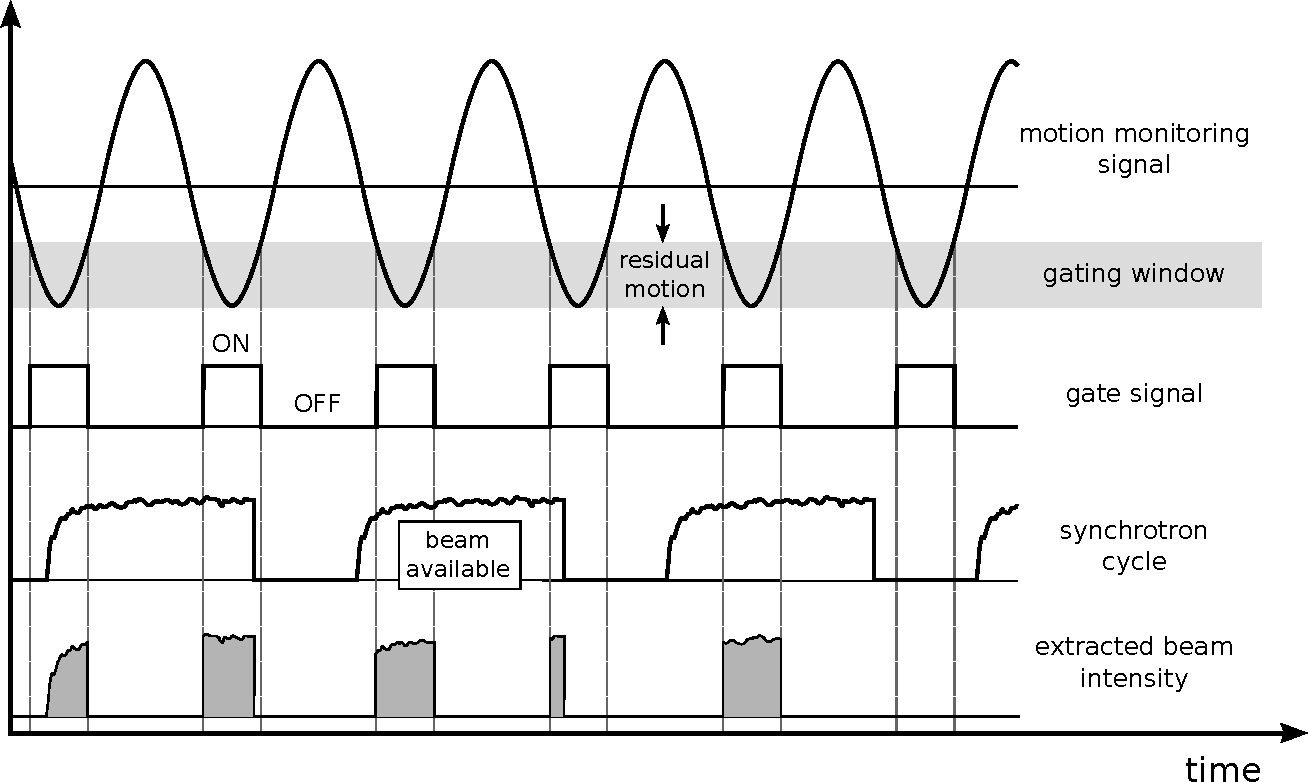
\includegraphics[width=0.9\textwidth]{./Fundamentals/Images/gatingscheme.pdf}
  \caption{Gating delivery with a synchrotron accelerator. The irradiation is only possible, when the gate signal is active and the beam is available. The gate signal
  depends on gating window and motion monitoring signal. Figure taken from \cite{Richter2012}.}
  \label{gating}
\end{figure}

\newpage
\begin{figure}[H]
\begin{center}
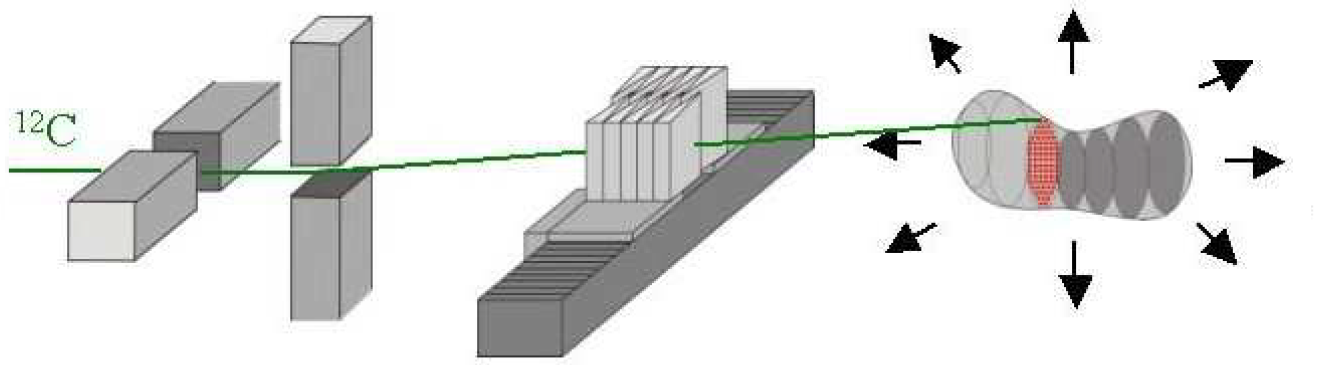
\includegraphics[width=0.9\textwidth]{./Fundamentals/Images/tracking.png}
\caption{Schematic presentation of GSI's beam tracking system. Two PMMA wedges, mounted on linear stepmotor, can change the energy of the beam traveling through. The changes in lateral direction are achieved via dipole scanner magnets. For the longitudinal adaptation two 
PMMA wedges are mounted on step motors, enabling to change the depth the particle beam has to traverse. Figure taken from \cite{Groezinger2004}}
\label{tracking}
\end{center}
\end{figure}

\subsection{Treatment planning}
\label{treatmentPlanning}

The task of treatment planning is to determine machine parameters in order to deliver prescribed dose to the target, while not violating maximum allowed dose to critical organs, also known as organs at risk (OARs) \cite{Richter2012}.
Treatment planning thus revolves around dose optimization process and it is highly dependent on delivery type used for treatment. The optimization problem for tumors can be written as:

\begin{equation}
  \min_{x} \sum_{i} \left( f(x,A_i) - D_{pre} \right)^2 
\end{equation}

Here $i$ is a CT voxel, function $f$ is a dose deposition model, $x$ intensity of the radiation beams, $A$ patient geometry and beam parameters and $D_{pre}$ is the prescribed dose.

The basis of treatment planning is a computed tomography (CT), where target volume and OARs are delineated
done by physician. Additional imaging, such as magnetic resonance (MRI) or positron emission tomography (PET), is often used as a supplement to CT for enhanced contrast of it. In the following sections, the target definition will be explained and the basics of scanned ion beam treatment planning. Afterwards an explanation on dose calculation for moving targets will be given.

\subsubsection{Target definition}
The definition of the target volume is crucial, since it has to cover the whole tumor, prevent further tumor spreading, while at the same time it should not be too big to spare normal tissue. 
The International Commission on Radiation Units (ICRU) recommends the following definitions for volumes used in treatment planning, which will also be used in this work, see Fig.~\ref{targets} \cite{ICRU50, ICRU62}.
\begin{description}
\item[Gross Tumor volume:] \emph{The GTV is the gross
    palpable or visible/demonstrable extent and location of malignant
    growth.}
\item[Clinical Target Volume:] \emph{The CTV is a tissue
    volume that contains a demonstrable GTV and/or subclinical
    microscopic malignant disease, which has to be eliminated. This
    volume thus has to be treated adequately in order to achieve the
    aim of therapy, cure or palliation.}
\item[Planning Target Volume:] \emph{The PTV is a geometrical
    concept, and it is defined to select an appropriate beam size and
    beam arrangements, taking into consideration the net effect of all
    the possible geometrical variations, in order to ensure that the
    prescribed dose is actually absorbed in the CTV.}
\item[Internal Target Volume:] \emph{This is the margin that must be
    added to the CTV to compensate for expected physio-logical
    movements and variations in size, shape, and position of the
    CTV during therapy.}
\item[Organs at risk:] \emph{Organs at risk (OAR) are normal
    tissues whose radiation sensitivity may significantly influence
    treatment planning and/or prescribed dose.}
\end{description}

\begin{figure}[H]
\begin{center}
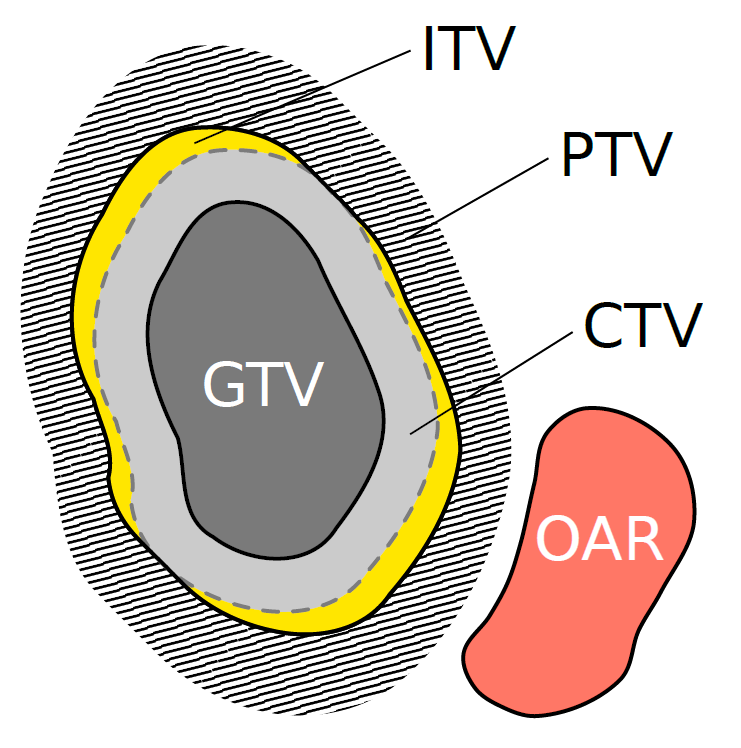
\includegraphics[scale=0.3]{./Fundamentals/Images/volumes.png}
\caption{ICRU treatment planning volumes definitions. Figure taken from \cite{Richter2012}}
\label{targets}
\end{center}
\end{figure}

Further recommendations of the ICRU state that 100\% of the PTV volume should receive between 95\% and 100\% of the planned dose \cite{ICRU50}.


\subsubsection{Treatment planning for scanned ion beams}

A treatment planning system (TPS) for active shaping ion beams has to model the active beam delivery system and the beam interactions with the tissue. Furthermore, for ions heavier than protons
the biological effectiveness and fragmentation must also be considered, which add additional complexity to the TPS. A TPS for beam scanning was developed at GSI, called TRiP98. The basic concepts of TRiP98 will be
presented here, further reading can be found elsewhere \cite{Kraemer2000,Kraemer2000a, Richter2013}.

TRiP98 divides PTV into energy slices, which are further divided into raster points in a defined order that the beam will follow. In the optimization step, a gradient-decent algorithm iteratively optimizes particle number
for each raster point, so that the optimal target dose is achieved. Dose can either be physical or biological, using LEM biological effectiveness (see Section~\ref{RBE}).
Physical characteristic of the beam include lateral scattering as proposed by Moli\`ere \cite{Moliere1948} and nuclear fragmentation that yield secondary particles. The patient specific
geometry and tissue inhomogeneities are accounted for using a transformation from CT HU to water-equivalent path length (WEPL) \cite{Geiss1999,Jaekel2001,Rietzel2007}.


\subsubsection{GSI's 4D treatment planning system}

As mentioned in section \ref{sec:motion} tumor motion can cause severe dosimetric errors. To asses dose deficiencies and to overcome them, TRiP98 was expanded to be able to calculate time-resolved (4D) treatment plans. The new software was named TRiP4D and a detailed description is given by Richter et al \cite{Richter2013}.

A static CT is not sufficient for 4D treatment planning. Time-resolved CT scans (4D-CT) therefore have to be used. 4D-CT consist of several quasi-stationary sections, called motion phases. Data is
recorded in each slice throughout the whole motion and is then sorted to appropriate motion phases, according to motion signal \cite{Rietzel2005}.

Besides a 4D-CT, a vital part of 4D treatment planning is \textbf{image registration}. It provides quantification of motion with deformation maps between different 4D-CT motion states. Image registration principles are described in Section~\ref{sec:registration}. The image registration is not included in TRiP4D, so an external software must provide the necessary
deformation maps.

The calculation of 4D dose starts with the division of the treatment plan into sub-plans, according to the motion phase it will irradiate. The number of sub-plans is the same as number of motion phases (or number of motion phases
in gating window, if gating is used). Afterwards the number of particles is calculated in each voxel of all of the motion phases used. Finally, the particle number in each voxel is transformed with the deformation maps
obtained from registration, to the reference phase, where the accumulated dose from summed particle numbers is calculated (see Fig.~\ref{TRiP4Ddose}). If biological dose is calculated, then instead beside particle numbers, energy spectra is also accumulated, 
so that the RBE can be calculated according to LEM for the total dose to each CT voxel.

\begin{figure}[H]
\begin{center}
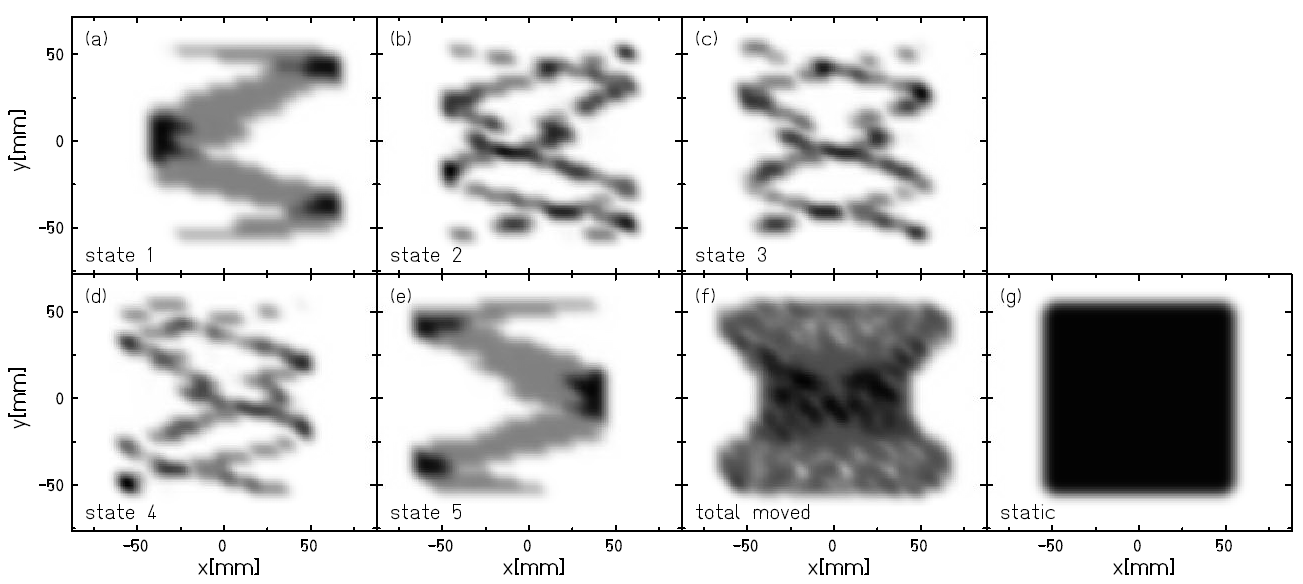
\includegraphics[scale=0.35]{./Fundamentals/Images/4DtreatmentPlanning.png}
\caption{Experimental validation of TRiP4D dose calculation on film response. On images a)-e) the individual dose deposition for the five motion states is showed.
Image f) shows accumulated 4D dose and image g) a homogeneous dose on a stationary film. Figure taken from \cite{Richter2012}}
\label{TRiP4Ddose}
\end{center}
\end{figure}

\subsubsection{Image registration}
\label{sec:registration}


Temporal changes in patient anatomy are assessed with image registration. Registration can be made between different imaging modalities (CT, MRI, PET), between scans from different days or between
different phases in 4D-CT. It requires two images: a fixed and a moving one. The result of the registration is a deformation map originating from the moving and pointing to the fixed image. Registration can be written as:


\begin{equation}
\label{df}
x' = x + u_{ri}(x)
\end{equation} 

Here, $x$ and $x'$ are points in states $r$ and $i$, respectively and $u_{ri}$ is a vector field representation of the transformation map. $u_{ri}$ can be used to assess motion amplitude, propagate contours and calculate 4D dose.
It is important to note that certain steps in 4D treatment planning require also inverse registration, from state $i$ to $r$ \cite{Richter2012}. If deformation map is applied to the moving image, 
the new image is called warped image and it should be as close to the fixed image as possible. Fixed, moving and warped image are shown in Fig.~\ref{RegistrationCompare}. 

\begin{figure}[H]
\begin{center}
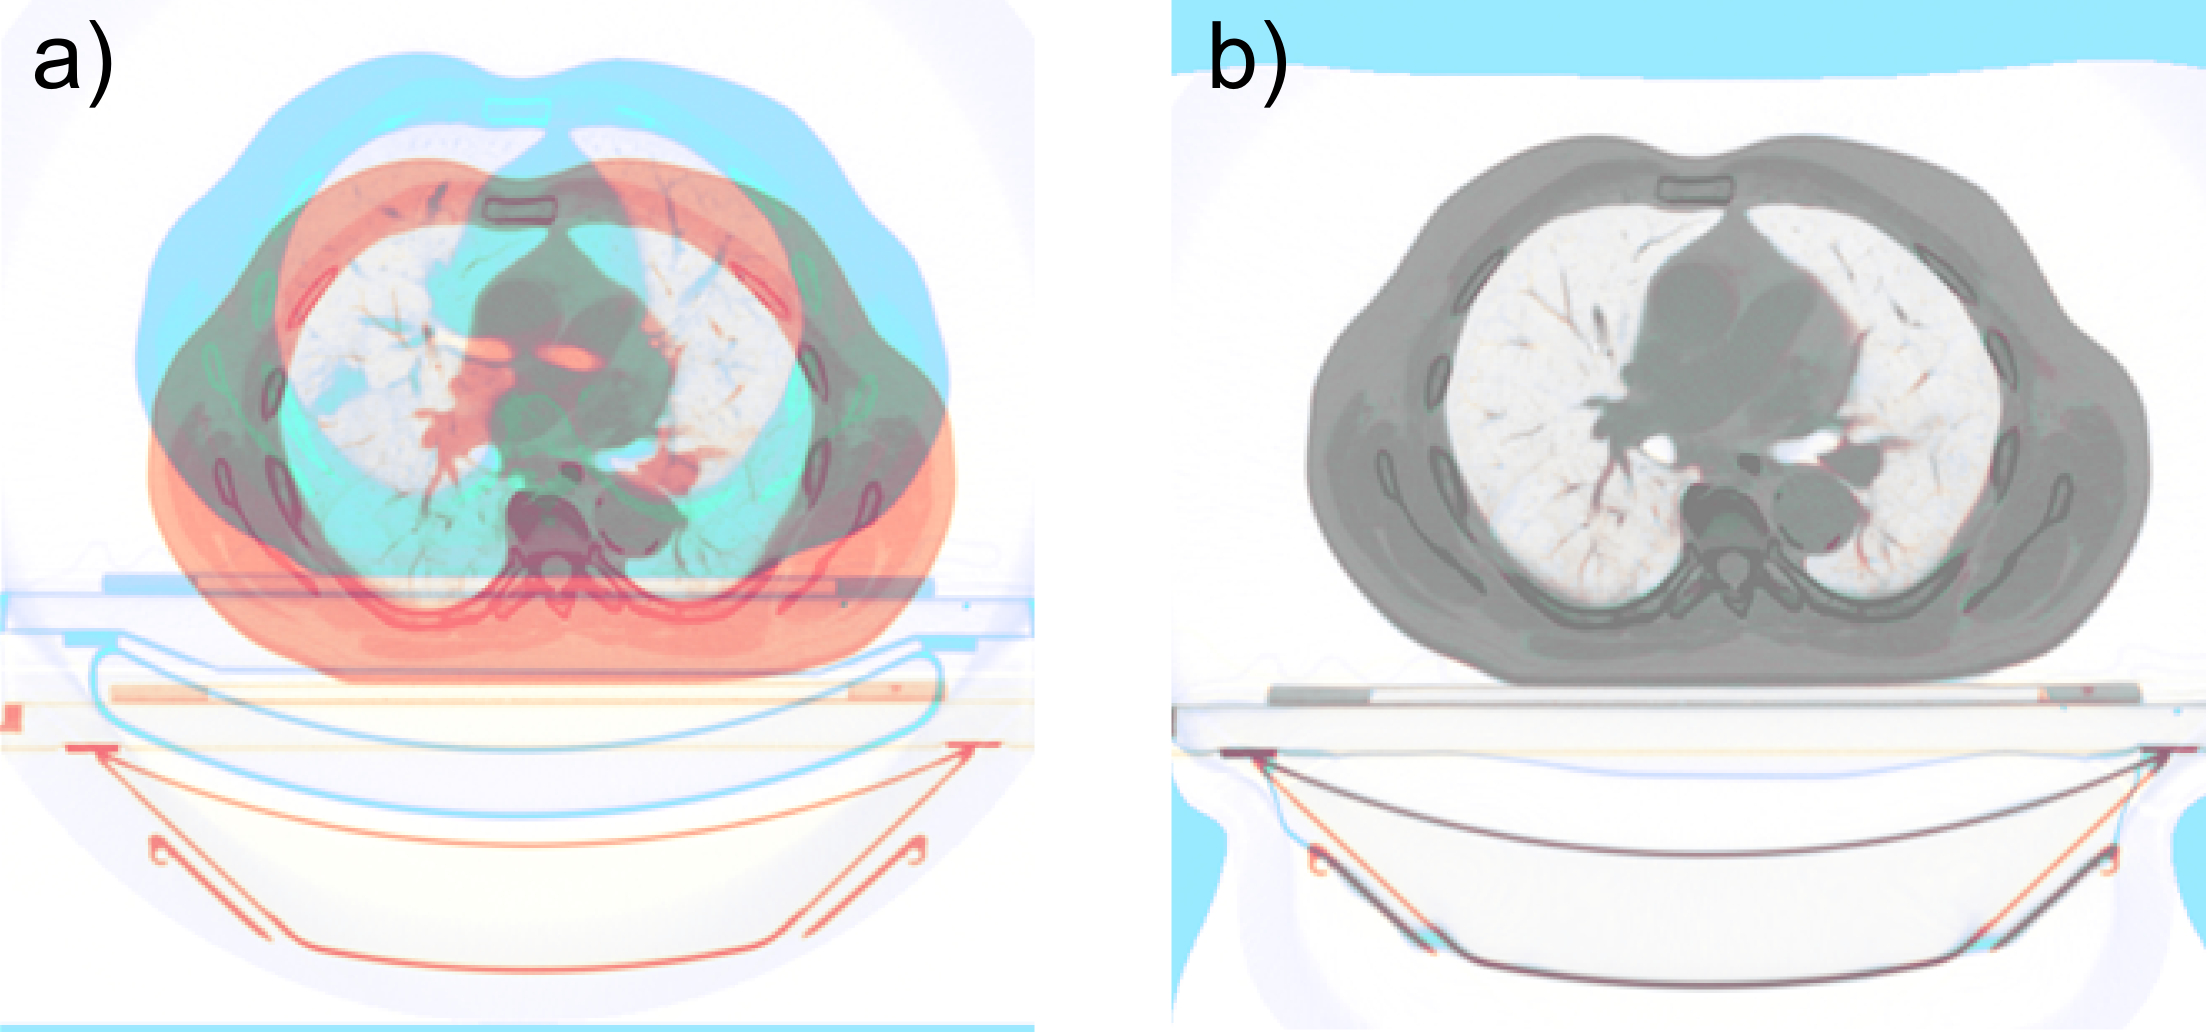
\includegraphics[width=0.9\textwidth]{./Fundamentals/Images/RegistrationCompare.png}
\caption{Overlap of fixed and moving image CT scan (a) and fixed and warped image after registration (b). Inverse colors are used in both CTs so that the overlayed image should be gray
where the images overlap perfectly.}
\label{RegistrationCompare}
\end{center}
\end{figure}

There are different possible types of registration and can be placed in two groups. First group consist of linear registrations: translation, rotation and scaling. In medical imaging the most commonly used linear transformation 
is translation or rigid registration. The other group of registrations are elastic or deformable registrations. The actual algorithms for performing registration are complex and the reader can
find detailed review elsewhere \cite{Hill2001,Brock2006,Rietzel2006a}. A multi-institutional study has shown that the accuracy for the majority of the algorithms is in the order of image voxel
size, i.e. millimeters \cite{Brock2010}. The study further states that the registration quality depends on image contrast. The quality of image registration is actually hard to quantitatively
asses and usually the registration results are checked visually. To improve image registration quality assurance a dedicated software was developed and is described in detail in chapter \textbf{REF}.

\newpage




\section{Lung cancer}

There were 1.8 million new lung cancer cases diagnosed worldwide in 2012 \cite{Worldwide2012}. With a very poor prognosis (5-year survival rates in Germany are
16\% for men and 21\% for women \cite{Kaatsch2014}) lung cancer is one of the most frequent and most deadly cancer types. Usually lung cancer is distiguised
into small-cell lung cancer (SCLC) and non-small cell lung cancer (NSCLC). Around 14\% of lung cancer cases are SCLC \cite{Tsao2008}, which is normally treated with chemotherapy and radiotherapy, while for NSCLC the traditional course of treatment
are surgery and radiotherapy. An example of cancerous lung tissue is shown in Fig.~\ref{Fig:Cancer}.

\begin{figure}[H]
\begin{center}
\includegraphics[width=0.7\textwidth]{./Fundamentals/Images/LungCancer.png}
\caption{Cross section of a human lung. The white area in the upper lobe is cancer, the black areas indicate the patient was a smoker. Figure taken from \cite{LungCancer}}
\label{Fig:Cancer}
\end{center}
\end{figure}


\subsection{Epidemiology}

The main cause for lung cancer is a long-term exposure to tobacco smoke \cite{Tsao2008}, with 85\% of cases contributed to smoking. There are over 70 known carcinogens in cigarette smoke, such as benzo[a]pyrene, 1,3-butadiene and a radioactive isotope of polonium, polonium-210 \cite{Hecht2012}. See Fig.~\ref{Fig:Smoking} for correlation between sales of tobacco products and rate of the lung cancer.

Studies have shown that passive smokers have an increased risk of lung cancer as well, with more then 20\% increase in risk for those who live with someone who smokes and 16-19\% increase for someone working with a smoker \cite{Taylor2007}.
There is some controversy weather smoking cannabis increases risk of lung cancer - two reviews from 2013 and 2014 have found contradicting results \cite{Tasckin2013, Underner2014}.

The other 15\% of lung cancer cases is attributed to a combination of genetic factors, exposure to radon gas, asbestos or other forms of air pollution \cite{Alberg2010}.

\begin{figure}[H]
	\begin{center}
		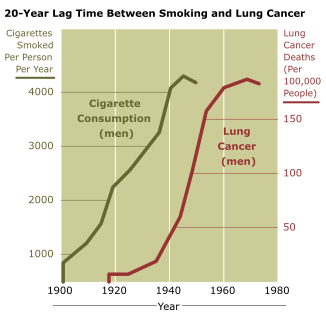
\includegraphics[width=0.7\textwidth]{./Fundamentals/Images/Smoking.png}
		\caption{Correlation between sales of tobacco products and the rate of the lung cancer in the USA between 1900 - 1970. Data released from National Cancer Institute.}
		\label{Fig:Smoking}
	\end{center}
\end{figure}


\subsection{Non-small cell lung cancer}

The NSCLC is divided into three main groups: adenocarcinoma, squamous-cell carcinoma and large-cell (undifferentiated) carcinoma \cite{Kasper2015}.
Between 25-35\% of all lung cancer cases are adenocarcinoma, squamous-cell carcinoma contributes to around 30\% of lung cases and 10-15\% are large-cell carcinoma. The SCLC contributes the rest. 

Lung cancer staging is used to refers to the extent to which the lung cancer has to spread from it's original source. Additionally, staging is used to establish treatment and prognosis \cite{Chheang2013}. For NSCLC, the TNM classification is used, which depends on
size of the primary tumor (T), involvement of the lymph node (N) and distant metastasis (M) \cite{Kasper2015}. According to the TNM class a group is assigned, from stage 0, IA, IB, IIA, IIB, IIIA, IIIB to IV. 
A schematic presentation of some stages is shown on Fig.~\ref{Fig:Stages}. Prognosis is highly dependent on stage, as shown in Table~\ref{tab:prognosis}.

\begin{table}[H]
  \centering
%   \footnotesize
  \caption{Five-year survival rates for different stage of NSCLC. Data taken from \cite{Rami2009}}
  \begin{tabular}{|c|c|}
   \hline
   \hline
Clinical stage & Five-year survival (\%) \\
IA & 50 \\
IB & 47 \\
IIA & 36 \\
IIB & 26 \\
IIIA & 19 \\
IIIB & 7 \\
IV & 2 \\
\hline
\hline
  \end{tabular}
  \label{tab:prognosis}
\end{table}

\begin{figure}[H]
\begin{center}
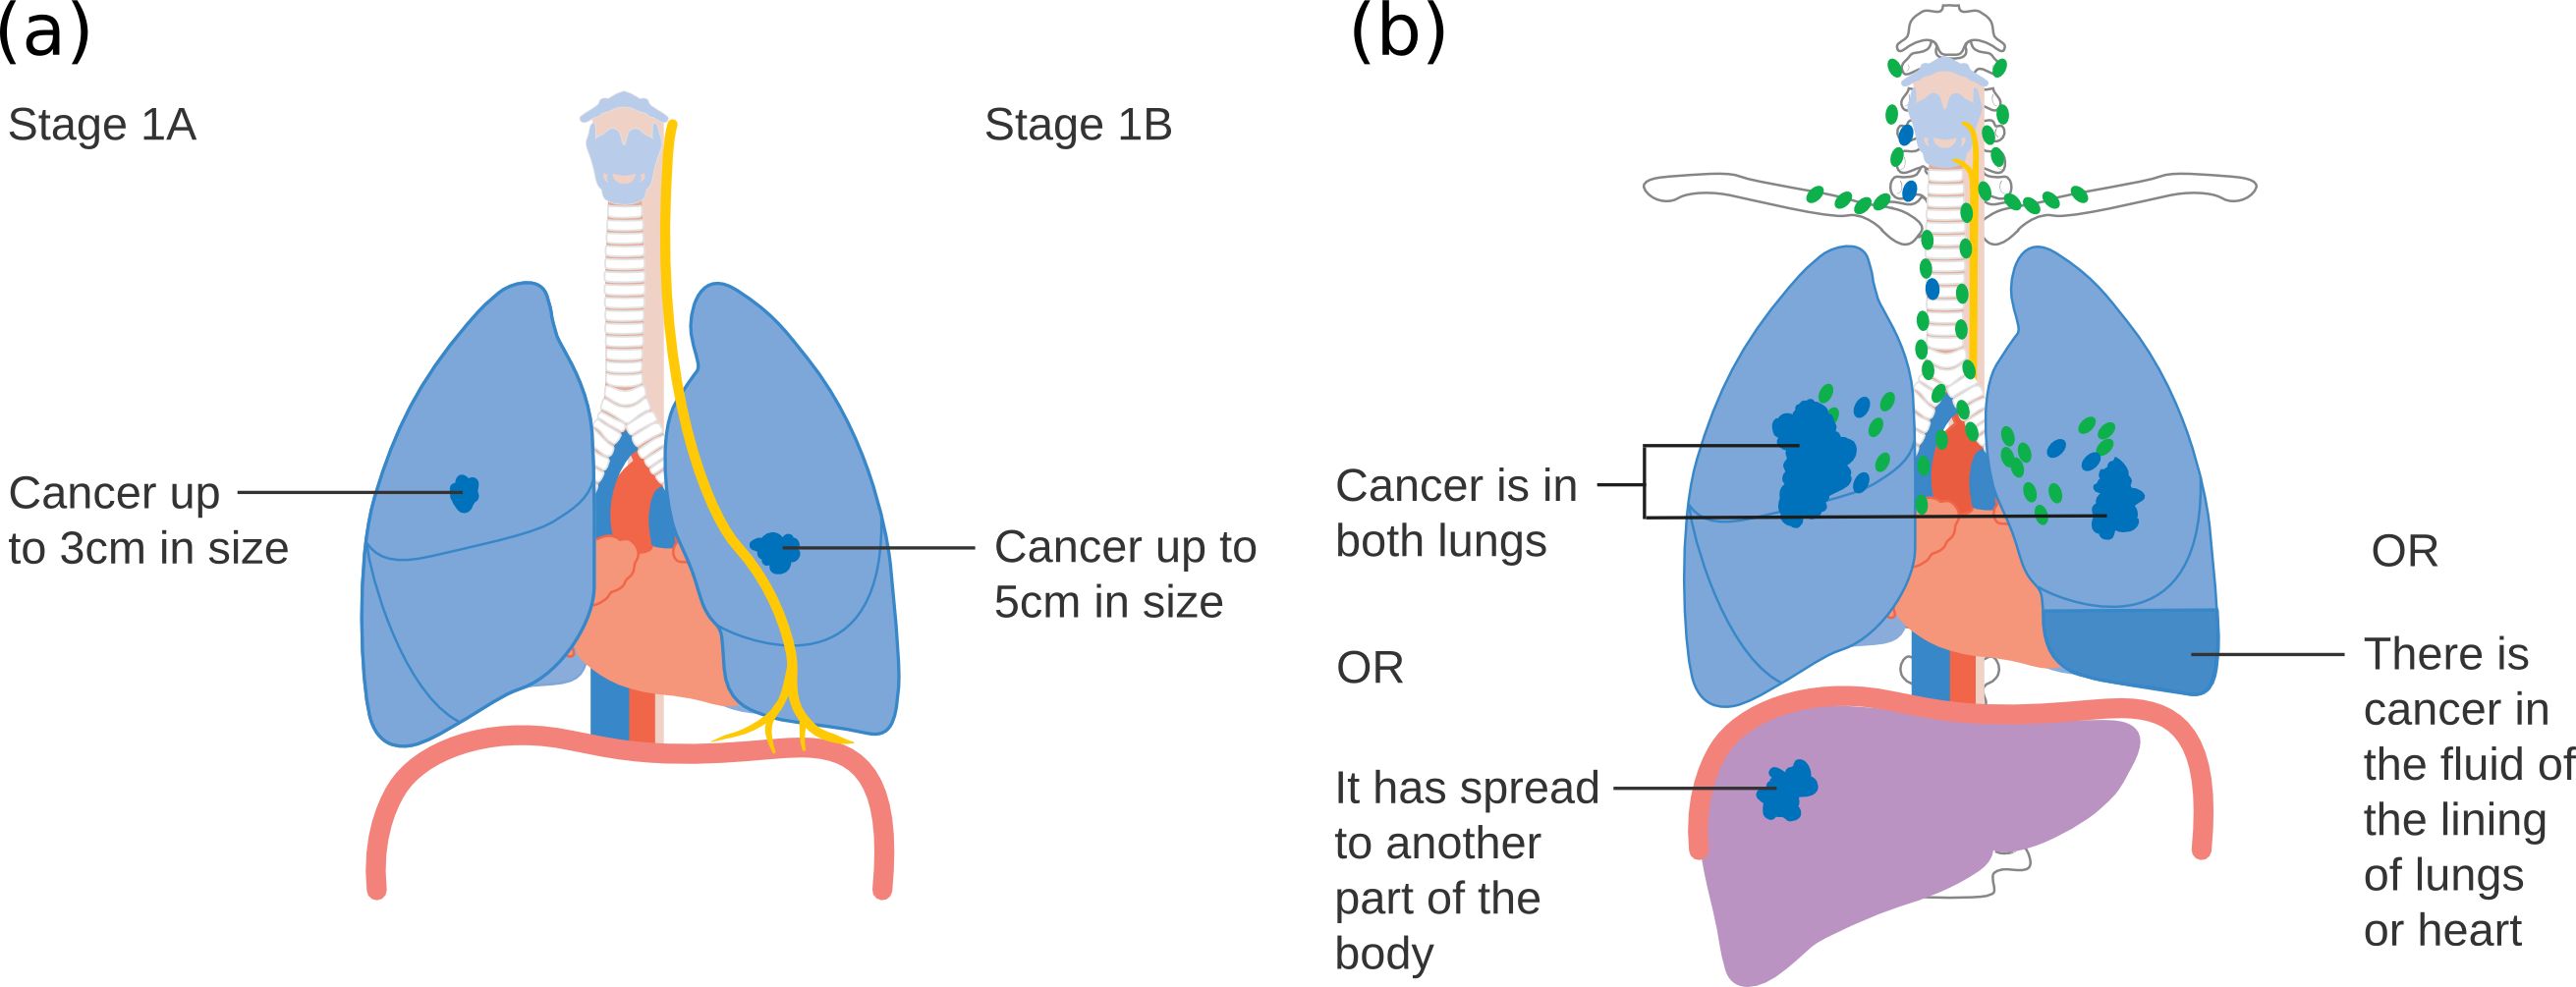
\includegraphics[width=0.9\textwidth]{./Fundamentals/Images/Stages.png}
\caption{Schematic presentation of three NSCLC stages. (a) Stages IA and IB; (b) Stage IV. Figure taken from \cite{CancerStage}}
\label{Fig:Stages}
\end{center}
\end{figure}

\subsubsection{Treatment}

The treatment for NSCLC can consist of surgery, chemotherapy, radiation therapy, or a combination of modalities. The treatment course depends on tumor type and stage and on patient overall condition
The typical treatment is surgery for stage I and II disease \cite{Tsao2008}. Surgery resection consist of either lobectomy or pneumonectomy, together with sampling lymph node or even a complete lymph node
dissection. Surgery will only be performed if NSCLC patients have enough lung reserve after lobe or lung is removed. The 5-year survival rate for NSCLC patients undergoing surgery is about 55 to 70\% 
and 35-55\% for stage I and II disease, respectively.

For unresectable stage III lung cancer the treatment consist of either chemotherapy or radiation therapy or a combination of both. The median survival for patients with unresectable stage IIIA disease is 10-14 months \cite{Tsao2008}.
For all treated stage IIIB disease the median survival is 7-15 months \cite{Srisam2005}.

Rather than treating stage IV disease, palliation of symptoms is the goal. With chemotherapy, targeted drugs and radiation therapy the tumor burden can be lessened and the quality of life can be improved. The prognosis is poor, with
median survival only 9 months and less then 25\% survive the first year after the disease is diagnosed \cite{Tsao2008}. Recent phase II trial combined chemotherapy with stereotactic body radiation therapy and 
showed promising results with 20 months overall survival \cite{Iyengar2014}.


  
  \setcounter{mtc}{2}
  \chapter{Deformable Image Registration and Validation}
\label{chapter:vmm}
\minitoc

\section{Introduction}

%As explained in Section \textbf{ref!}, effects of motion can have a significant impact on a radiation treatment. There are several motion mitigation techniques available that can operate on beam delivery, patient immobilization or treatment planning level.

Today most modern clinics regularly use different imaging techniques including CT, 4D-CT, cone-beam CT, MRI and PET. A registration is needed to overlay different image acquisitions, such as images taken at different days,
between different imaging modalities or to quantify anatomical changes in a time-resolved image acquisition, such as 4D-CT, 4D-MRI or 4D ultra sound. While most commercial treatment planning software provide rigid registration between different images, deformable image registration (DIR) is currently rarely used. 
DIR can quantify anatomical and biological variations better compared to rigid registration \cite{Sarrut2006}. It opens exciting new options in radiotherapy, such as 4D optimization \cite{Trofimov2005}, 
4D dose calculation \cite{Flampouri2006} or contour propagation \cite{Lu2006b}. 4D dose calculation has been well established for photons \cite{Ong2016}, protons \cite{Paganetti2005} and carbon-ions \cite{Gemmel2011} and has received
several experimental verifications \cite{Vinogradskiy2009, Perrin2016, Bert2012a}. 

A 4D dose calculation requires DIR for the deformation of the dose distributions in each motion state
to the reference state, where the dose from all motion states is accumulated. 4D dose calculation requires accurate DIR at every voxel, since errors in DIR can significantly alter the 4D dose \cite{Heath2006}. Special consideration has to be paid to calculation of biological 4D doses \cite{Gemmel2011}. 

Contours can be propagated in two ways - either with DIR \cite{Lu2006a, Rietzel2005a} or
with deformable model driven techniques \cite{McInerney1996}, which uses a physical model to iteratively match the contour to image features. In contrast to a 4D dose calculation, contour propagation requires accurate DIR at the contour boundaries.

Besides radiotherapy, DIR is used also in other medical fields \cite{Cleary2010, Herrell2012, Nithiananthan2011, Naini2010}.
Several different DIR algorithms are available, such as B-spline \cite{Rueckert1999}, Demons \cite{Thirion1998}, linear elastic finite element \cite{Venugopal2005}, optical flow \cite{Zhong2007} or viscous fluid \cite{Christensen1996}.
	
The DIR has a large degrees of freedom and as such is an ill-posed problem and hence prone to errors. The errors can result in image misalignments or in physically impossible vector fields. 
One of the reasons why DIR is not commonly used in commercial softwares is the lack of proper DIR quality assurance (DIRQA), which is essential for implementation of DIR in the clinical work-flow. While several different DIRQA methods exist, none of them are definitive and most of them are time consuming. 
It is possible to evaluate DIR with deformable phantoms, where the type and size of deformation is known \cite{Kashani2007, Kirby2011}. However this effort is prohibitive 
in the everyday clinical work flow. DIR validation can also be based on landmark positions, specifically their location before and after registration. In absence of externally planted markers, locating landmarks in the patient 
anatomy can be time-consuming and it can be difficult to identify landmarks in low-contrast regions \cite{Varadhan2013}. Another option is to compare delineated contours with the propagated ones using the dice similarity coefficient \cite{Varadhan2013} or Hausdorff distance \cite{Huttenlocher1993}. 
While more efficient than landmark checks, these techniques require additional delineation and do not address the region within the contour.

A set of tools was created to systematically handle DIR and DIRQA in the open-source software 3D Slicer. Tools were tested on a large data set to verify their validity.

\section{Implementation}
\label{Implementation}

\subsection{3D Slicer}
\label{Slicer}

3D Slicer (Slicer) is a software platform for the analysis and visualization of medical images \cite{Slicer, Fedorov2012}. Slicer is a free, open-source software (BSD-style license) available on Windows, MacOSX and Linux operating systems. 
It comes with a vast variety of tools, such as:

\begin{itemize}
	\item Handling all commonly image formats, including DICOM, NRRD and MHA
	\item Visualization of voxel images, polygonal meshes and volume renderings
	\item Image registration (rigid and non-rigid) and display of vector fields
	\item Automatic image segmentation
	\item Analysis and visualization of diffusion tensor image data
	\item Device tracking for image-guided procedures
\end{itemize}

The source code of Slicer is written in C++ and with a Python wrapper to provide rapid, iterative development. The graphical user interface is based on Qt. The visualization is based on VTK \cite{Vtk}, a graphical library commonly
used in scientific research.

Slicer is a research tool and as such allows implementation of new functionalities in the form of extensions (modules). They can either be as external command-line programs, 
as scripts to automate Slicer processes or as unique modules with new features. 

\subsection{Registration}
\label{RegistrationImplement}

Plastimatch \cite{Shackleford2010} is a commonly used software for registration in medical research. It is a free and open-source tool, available as a command-line executable program. 
Plastimatch B-spline registration is also available in Slicer as part of the extension SlicerRT \cite{Pinter2012}.
The integration of Plastimatch in Slicer brings the advantage of a graphical user interface, offering a quick modification of parameters and visualization of the results. 
However, automation is needed for a large number of registrations. For a complete 4D-CT registration there are $2(N-1)$ registrations required - from the reference phase to each of $N$ motion states of 4D-CT and vice versa, except for the reference phase itself. 
Typical 4D-CTs consist of 10 phases, therefore automated registration of a 4D-CT is necessary.

The automated DIR was achieved with a Python class to handle image locations, store DIR parameters, perform DIR in the Plastimatch module, use correct naming conventions and store all output files (vector fields and warped images). 
Details can be found in Appendix~\ref{AppendixA}.



\subsubsection{Registration nomenclature}

To provide a clear and consistent description of methods used, an overview of the expressions is given here.

\begin{itemize}
 \item \textbf{Reference image} - the image that serves as a reference position in registration (image that is being registered to).
 \item \textbf{Moving image} - the image that is matched to the reference image (image that is being registered from).
 \item \textbf{Warped image} - the result of applying a transformation map from registration to the moving image. It should be as close to the reference image as possible.
 \item \textbf{True registration} - the registration from the moving to the reference image. Similar, everything connected to the true registration will use ``true'' (true vector field, true warped image, true absolute difference, true Jacobian, etc.).
 \item \textbf{Inverse registration} - the registration from the reference to the moving image (opposite or inverse of the true registration). As in the true registration, the term inverse can be used for everything connected to it (inverse vector field, inverse warped image, inverse absolute difference, inverse Jacobian, etc.).
\end{itemize}

In radiotherapy the true registration is used for dose propagation and consequential the 4D Dose calculation, whereas with the inverse registration contours can be propagated from the reference to the moving phase.


\subsection{Registration Quality Checks}
\label{DIRQA}

In order to provide visual and quantitative assessment of the registration quality a \textbf{Deformable Image Registration Quality Assurance} or DIRQA module was created. 
It provides image checks (inverse color, checkerboard, absolute difference, flicker, movie and landmark distances) 
and vector checks (Jacobian and inverse consistency error). 
The reference and warped image, true and inverse vector are used as inputs for the DIRQA module. 
Additionally, landmarks and a region of interest (ROI) can also be used as an input.

Tests can be divided into two groups: qualitative (inverse color, checkerboard, flicker, movie) and quantitative 
(absolute difference, landmark distances, Jacobian and inverse consistency error) tests.
Absolute difference, Jacobian and inverse consistency error tests
were build using tools from the ITK library \cite{Yoo2002}.

\subsubsection{Qualitative tests}

A DIR quality can be assessed with visual inspection of DIR results. Several tests were developed to make the visual inspection easier.

\newpage
\subsubsection{Inverse color}


Overlaying two different images will highlight the difference between them. However, since CT scans are usually displayed in grayscale color code, the differences can be indistinguishable. 
Especially if the images are quite similar, as the reference and the warped image should be. With applying opposite color codes to overlaying images two things are achieved. 
First, regions where the registration was successful will be in grayscale. Second, the differences between images will be highlighted in the color of the image they originate from. 
In the module we used red and cyan color code for reference and warped image, respectively. See Fig.~\ref{falseColor} for details.

\begin{figure}[H]
	\begin{center}		
		\includegraphics[width=0.9\textwidth]{./Vmm/Images/falseColor.png}
		\caption{An example of a inverse color overlay. Images (a) and (b) show red and cyan color code, respectively, for a CT scan. (c) displays overlayed inverse colored images before and (d) after registration.}
		\label{falseColor}
	\end{center}
\end{figure}

\subsubsection{Checkerboard}

As the name suggests, checkerboard creates an image of tiles. Each tile alternates between the reference and the warped image, as shown in Fig.~\ref{checkerboard}. The differences between two images become apparent if there is no smooth transition from one tile to the next. 
The number of tiles can be manually selected.
\newpage
\begin{figure}[H]
	\begin{center}		
		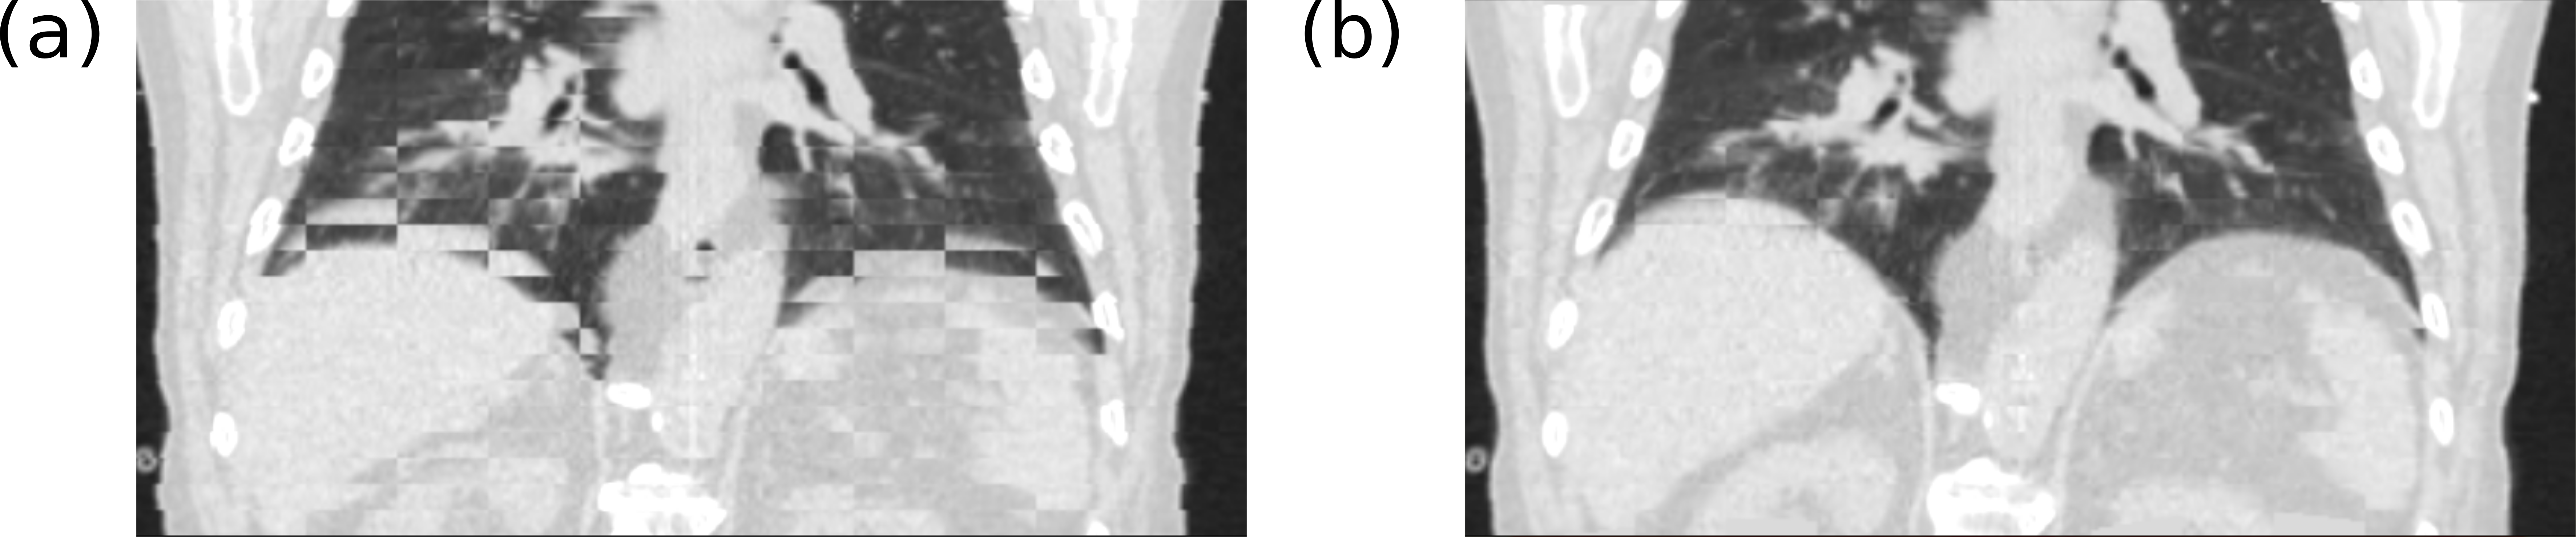
\includegraphics[width=0.9\textwidth]{./Vmm/Images/checkerboard.png}
		\caption{An example of a checkerboard image. It consists of tiles alternating between two images. Tiles in image (a) alternate between scans before registration and in image (b) after registration.}
		\label{checkerboard}
	\end{center}
\end{figure}

\subsubsection{Movie}

Medical images are usually quite large - a typical CT image consist of $512 \times 512 \times 100$ pixels, which makes inspecting image checks (inverse color, checkerboard, absolute difference) a time-consuming task. 
The movie feature allows a smoother display of different image slices. 
The user selects which view to inspect (axial, sagital or coronal) and presses start. Selected views then start scrolling from the first to the last slice of selected view. It allows user to focus on registration details, rather than scrolling through slices.



\subsubsection{Flicker}

While it is possible to display two images side by side in Slicer, it can sometimes be hard to see fine differences between the two images. Flicker alternates between reference and warped image on a single display at a 0.5 s rate. It allows
a quick inspection of differences between two images in their original form.

Movie and flicker (explained in the next section) do not offer any specific registration checks, but improve the process of DIRQA.

\subsubsection{Quantitative tests}

It can be hard to visually inspect all the DIR results, especially in a 4D-CT registration. Therefore a series of tests were developed that give a quantitative assessment of DIR quality.

\subsubsection{Absolute difference}

To stress the difference between reference and warped image an absolute difference between voxel values is calculated and displayed. 
A new image is generated with voxels populated as the absolute difference between reference and warped image voxel values, as shown in Fig.~\ref{absDiff}.
Furthermore, statistical values of absolute differences are calculated (mean, standard deviation, minimum and maximum) 
for a quantitative assessment of the registration quality (in the ideal case all values would be 0).

Three absolute differences can be calculated: between reference and moving image, called default absolute difference; between true warped and reference image, called true absolute difference; between inverse and moving image, called
inverse absolute difference. Usually, registration works on minimizing the absolute difference (mean square error metric), so it is a direct indicator
of registration success.

To save computational time or to focus on a specific region, the absolute difference can also be calculated just on a specific ROI (if used as an input). Usually the patient body is selected as ROI, without air and couch.


\begin{figure}[H]
	\begin{center}		
		\includegraphics[width=0.9\textwidth]{./Vmm/Images/abs.png}
		\caption{An absolute difference image before (a) and after registration (b). The mean absolute difference before registration (default absolute difference) is 62 HU and 31 HU after registration (true absolute difference).}
		\label{absDiff}
	\end{center}
\end{figure}


\subsubsection{Landmark distances}

Distances between landmarks before and after registration are often used to determine the spatial accuracy of registration \cite{Castillo2009}. 
Landmarks can either be a specific feature in the patient anatomy or an external marker. The position of landmarks in the warped image would ideally 
be at the same position as in the reference image. The module measures the Euclidean norm between the landmark positions in reference and warped image.

The user has to manually select landmarks in reference and moving or also in the warped image. For landmarks based on the patient anatomy, a selection from physician is required. 
Landmarks from the moving image can then be automatically transformed to the warped image using the registration vector field. An example is shown in Fig.~\ref{landmark}.
\newpage

\begin{figure}[H]
\begin{center}
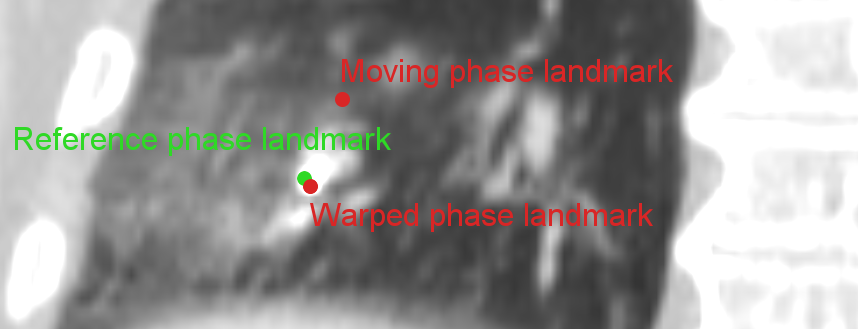
\includegraphics[width=0.7\textwidth]{./Vmm/Images/landmark.png}
\caption{A display of landmarks in three phases - reference, moving and warped phase. The distance before registration (between reference and moving landmark) is 22 mm and after registration
(between reference and warped landmark) is 2 mm.}
\label{landmark}
\end{center}
\end{figure}


\subsubsection{Jacobian determinant}
\label{Jacobian}

The Jacobian determinant or Jacobian ($J$) of the vector field $u$ is calculated as:



\begin{equation}
J = \begin{vmatrix} 
\frac{\partial u_x}{\partial x} & \frac{\partial u_x}{\partial y} & \frac{\partial u_x}{\partial z} \\
\frac{\partial u_y}{\partial x} & \frac{\partial u_y}{\partial y} & \frac{\partial u_y}{\partial z} \\
\frac{\partial u_z}{\partial x} & \frac{\partial u_z}{\partial y} & \frac{\partial u_z}{\partial z} \\
\end{vmatrix}
\end{equation}

The Jacobian is used to validate the physical behavior of the registration \cite{Leow2007}. 
The Jacobian of a vector field should be positive, since negative Jacobian values correspond to organ folding, 
which is physically unrealistic for patient anatomy \cite{ Rey2002, Chen2008}. 
Expansions and contractions around a point are indicated by Jacobian values greater or lower than 1, respectively.

The DIRQA module calculates and displays the Jacobian of the vector field, as shown in Fig.~\ref{JacobianImage}.
Statistical values of the Jacobian are also calculated. Similar to the absolute difference, the Jacobian can be calculated inside a ROI rather than on the whole image.
\newpage
\begin{figure}[H]
	\begin{center}		
		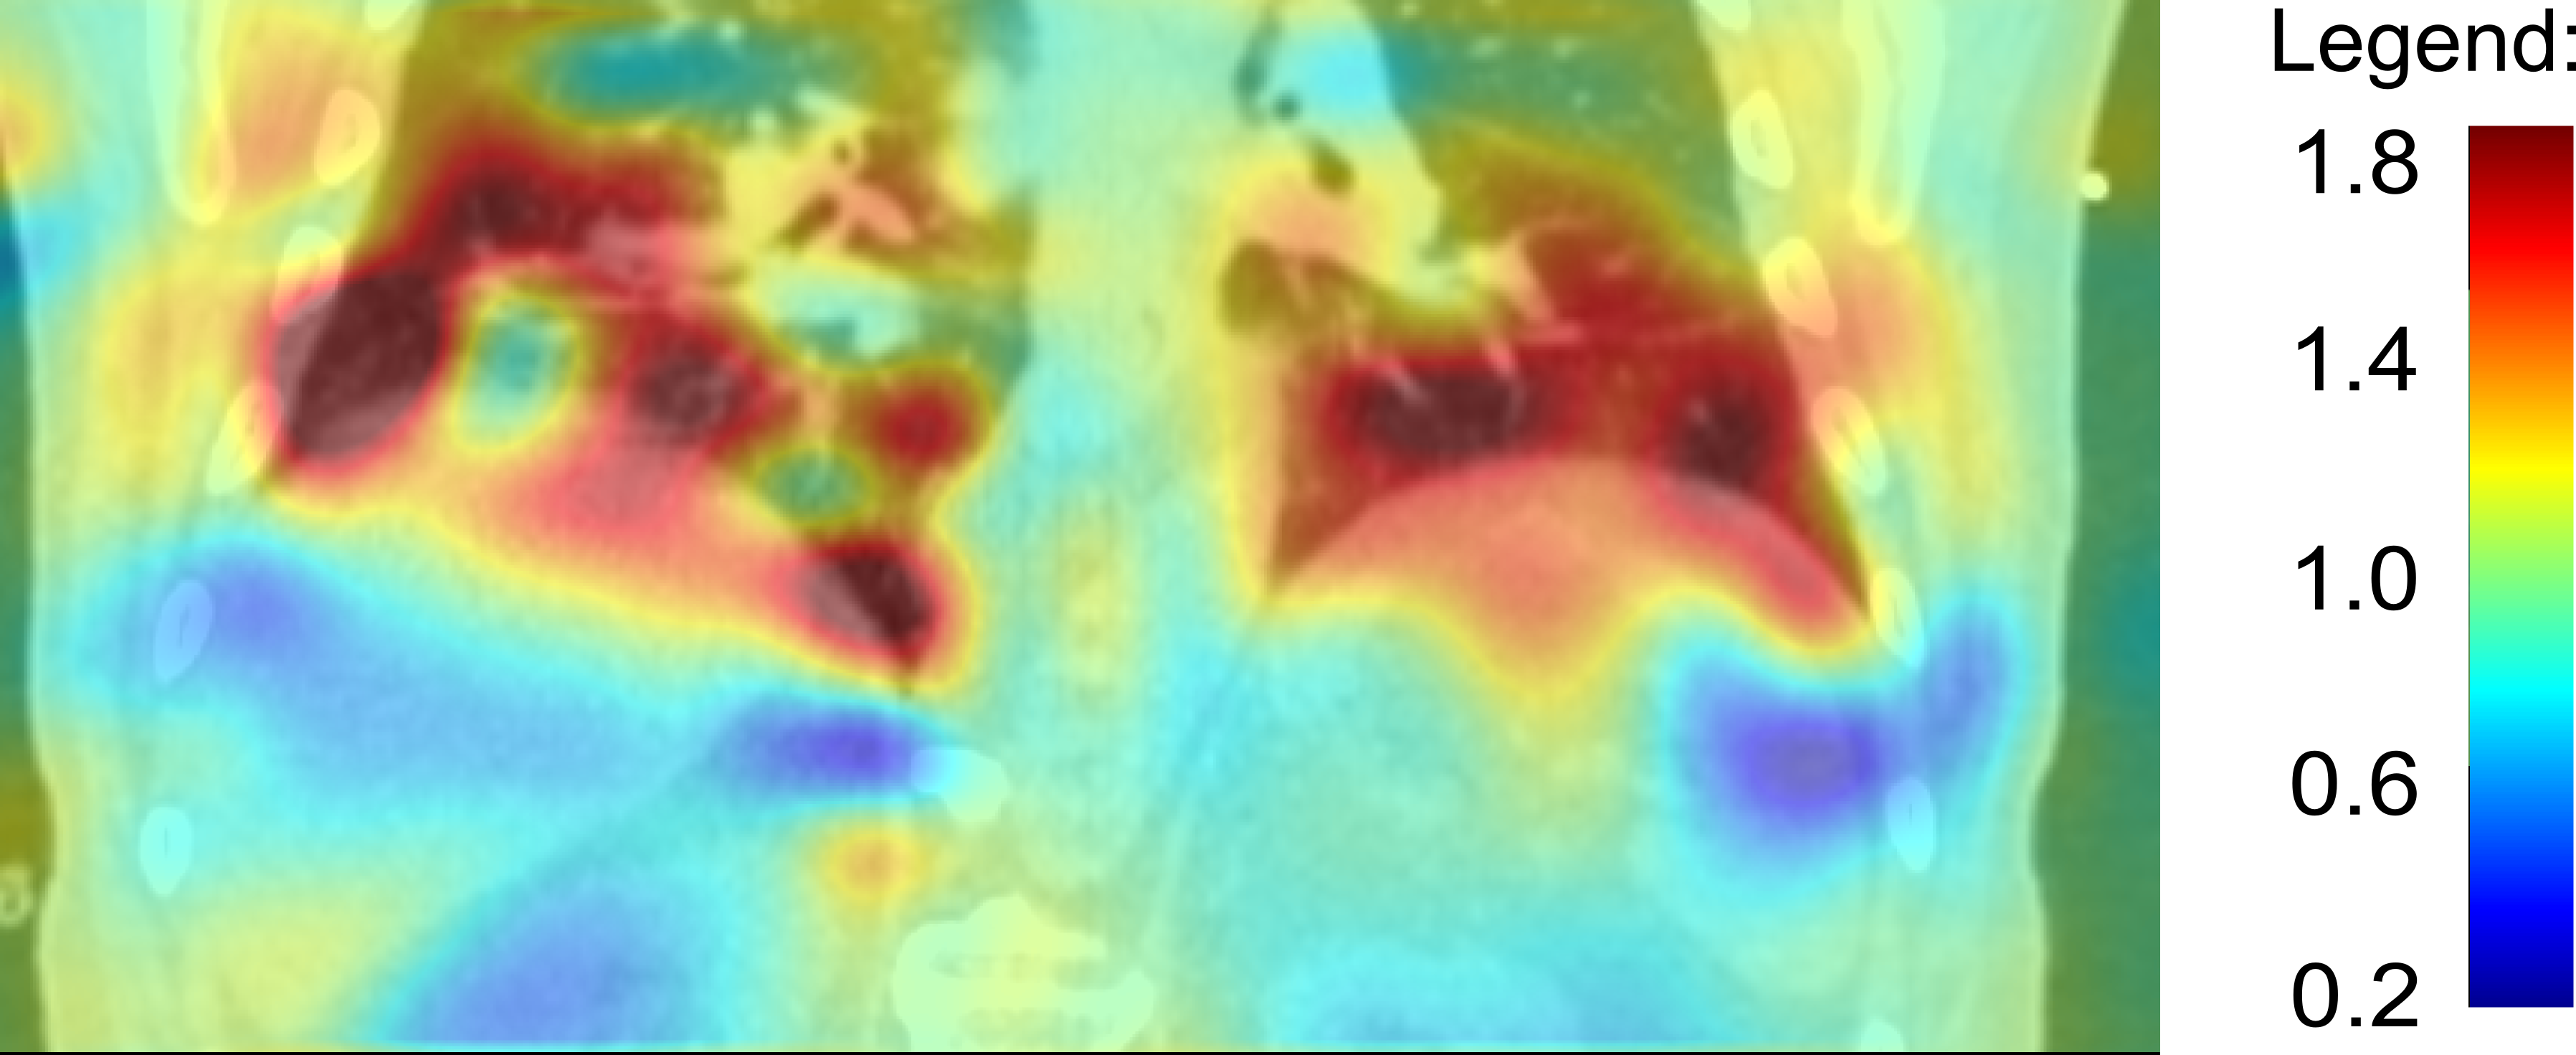
\includegraphics[width=0.8\textwidth]{./Vmm/Images/jacobian.png}
		\caption{An image of the Jacobian values overlayed on a CT scan. The average value of the displayed Jacobian is 0.98 with 0.09 standard deviation.}
		\label{JacobianImage}
	\end{center}
\end{figure}

\subsubsection{Inverse Consistency Error}
\label{ICE}

The inverse consistency error (ICE) is consistently used in literature as one of the main vector field checks \cite{Christensen2001, Bender2009}. The principle is as follows. 
Suppose we have two vector fields: $u_{AB}$ obtained from registration of image $A$ to $B$ and $u_{BA}$ from registration of image $B$ to $A$. The two registrations
are performed separately. In an ideal scenario, $u_{AB}$ would be a direct inverse of $u_{BA}$. However, DIR algorithms do not yield perfectly inverse consistent vector fields. Therefore, the differences between true and inverse vector fields have to be examined.


To check for ICE, an algorithm was created that first transforms a point $x$ in image $A$, using $u_{AB}$. The newly obtained point $x'$ is then transformed with the inverse vector
field, $u_{BA}$ which yields $x''$. The ICE is defined as Euclidean norm between $x$ and $x''$:

\begin{equation}
\label{eq:ice}
ICE = |x - x''| = |x - u_{BA}(x')| = |x - u_{BA}(u_{AB}(x))|
\end{equation}

Points $x'$ and $x''$ can have an arbitrary position in space, while vector fields $u_{AB}$ and $u_{BA}$ are positioned on a grid. To apply the transformation $u_{BA}(x')$, $x'$ is interpolated on a $u_{BA}$ grid. A tri-linear interpolation is used in this module.

As for the Jacobian, ICE image is calculated and displayed, along with statistical values and ROI feature. An example is shown in Fig.~\ref{inv}.




\begin{figure}[H]
\begin{center}
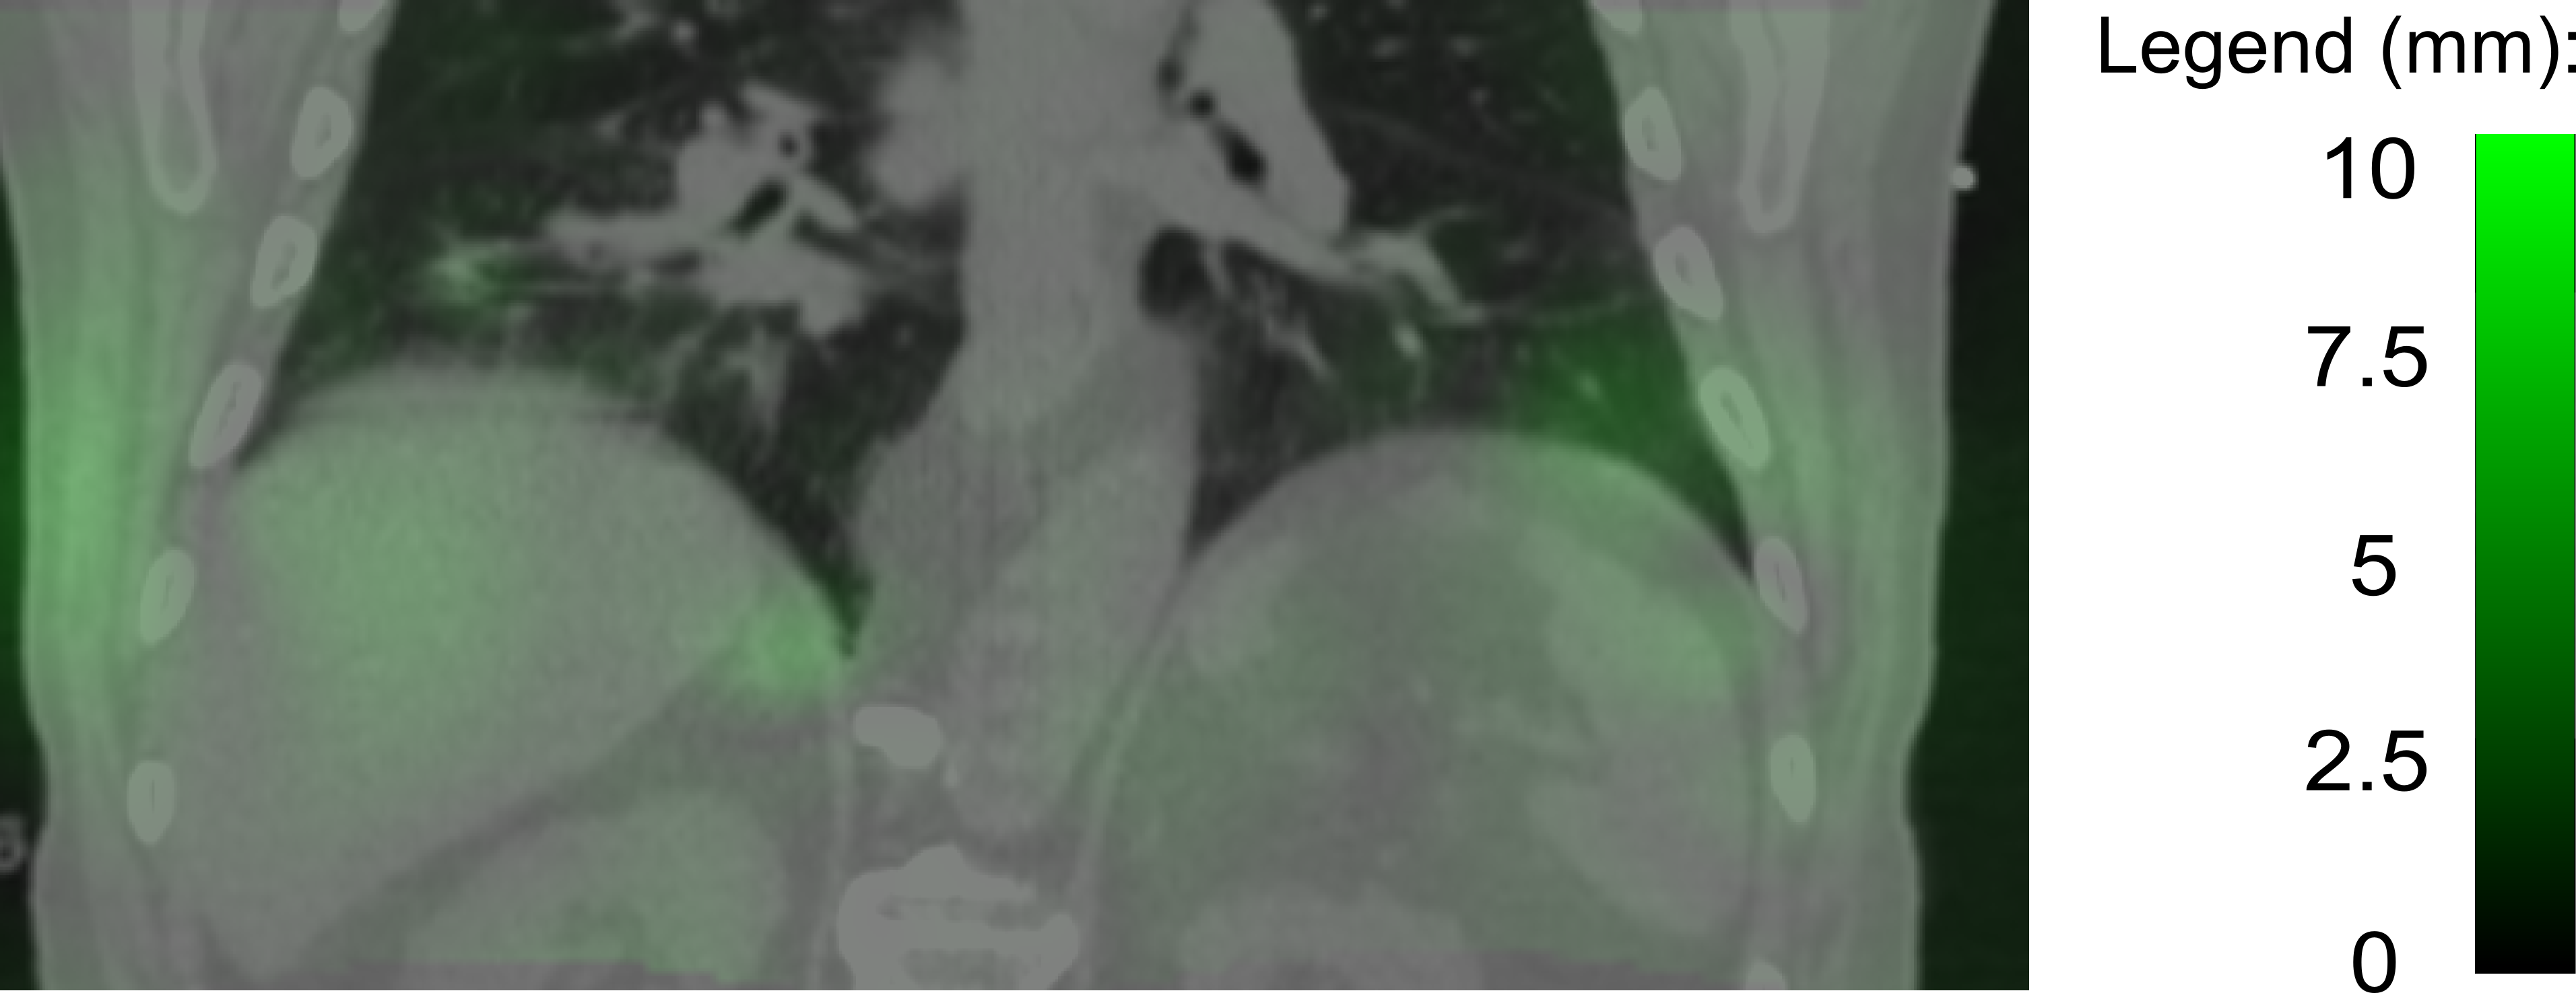
\includegraphics[width=0.8\textwidth]{./Vmm/Images/inv.png}
\caption{An image of the inverse consistency error (ICE) overlayed with CT scan. The average value of displayed ICE is 1.0 mm with 0.8 mm standard deviation.}
\label{inv}
\end{center}
\end{figure}


% \subsubsection{Output file}
% 
% With all different features to validate DIR it can be time consuming to go through them all. A special option was created to automatically go through all different validation steps. Furthermore it can also run through different phases, if there are more phases (i.e. in 4D-CT). All produced data from DIR validation is stored on disk and can be reexamined by user upon request. Furthermore, images are created and data is summed up and displayed in a separate file. Users can then preview file for first validation of DIR and then open necessary files, if required.

% \subsection{Contour visualization}
% \label{Contour}
% 
% TRiP4D (see Section \textbf{REF}) introduced volume datasets for contour representation \cite{Richter2012}. It enabled necessary tasks for 4D calculations, such as the storing contour in different 4D states, contour propagation, etc. However, there was a lack of a proper visualization tool. In order to provide a contour visualization tool, a Slicer module was created. 
% 
% Contours are saved as volumetric boolean masks. A single bit per ROI contour representation marks each voxel inside volume dataset \cite{Richter2012}. To properly display contour, first a whole volume dataset was imported in Slicer. User selects which motion state he would like to inspect. The corresponding bit is then selected on the imported volume dataset. Lastly the contour is converted into 3D model shape. 
% 
% \subsection{Motion estimation and ITV creation}
% 
% ITV is often created by an eye investigation of all 4D-CT phases, where the extent of motion is estimated. Automatic creation of ITV is scarce in commercial system, since it requires DIR on all 4D-CT phases. A Slicer module was created to assist with the motion estimation and automatic ITV creation using DIR. 
% 
% Module is able to estimate and display motion of a user selected contour in three axis (left-right, anterior-posterior, superior-inferior) based on DIR vector fields. Module also performs DIR on 4D-CT with patient hierarchy, if it has not been done yet.
% 
% Beside motion estimation, module can also propagate selected contour (usually CTV) and propagate it to all 4D-CT and make a convolution of all propagated contours, resulting in automatically generated ITV.
% 
% \subsubsection{Generation of mid-position phase}
% 
% Most commercial software calculates treatment plan on a single 3D CT scan, using 4D-CT only for motion estimation. To incorporate patient-specific motion information, a 3D CT scan was created from 4D-CT in the time averaged position, also known as mid-position scan (midP scan) \cite{Wolthaus2008}. With midP scan commercial software can still be used. Additionally, it also enabled smaller error margins for PTV generation and midP scan has less noise as individual 4D-CT scans, because it uses more data. 
% 
% Construction of a midP begins with registration of whole 4D-CT. The resulting vector fields from reference position to 4D-CT phases are then averaged to obtain mean vector field, see Fig.~\ref{midPgeneration}. Afterwards, for each vector field the mean vector field was subtracted, yielding a set of mean-corrected vector fields pointing from mean position to corresponding 4D-CT phase. The mean-corrected vector fields were finally inverted and applied to each 4D-CT phase, resulting in each phase being in the same, time-averaged position. In the end the set of transformed 4D-CT phase was averaged to obtain midP scan.
% 
% \begin{figure}[H]
% \begin{center}
% 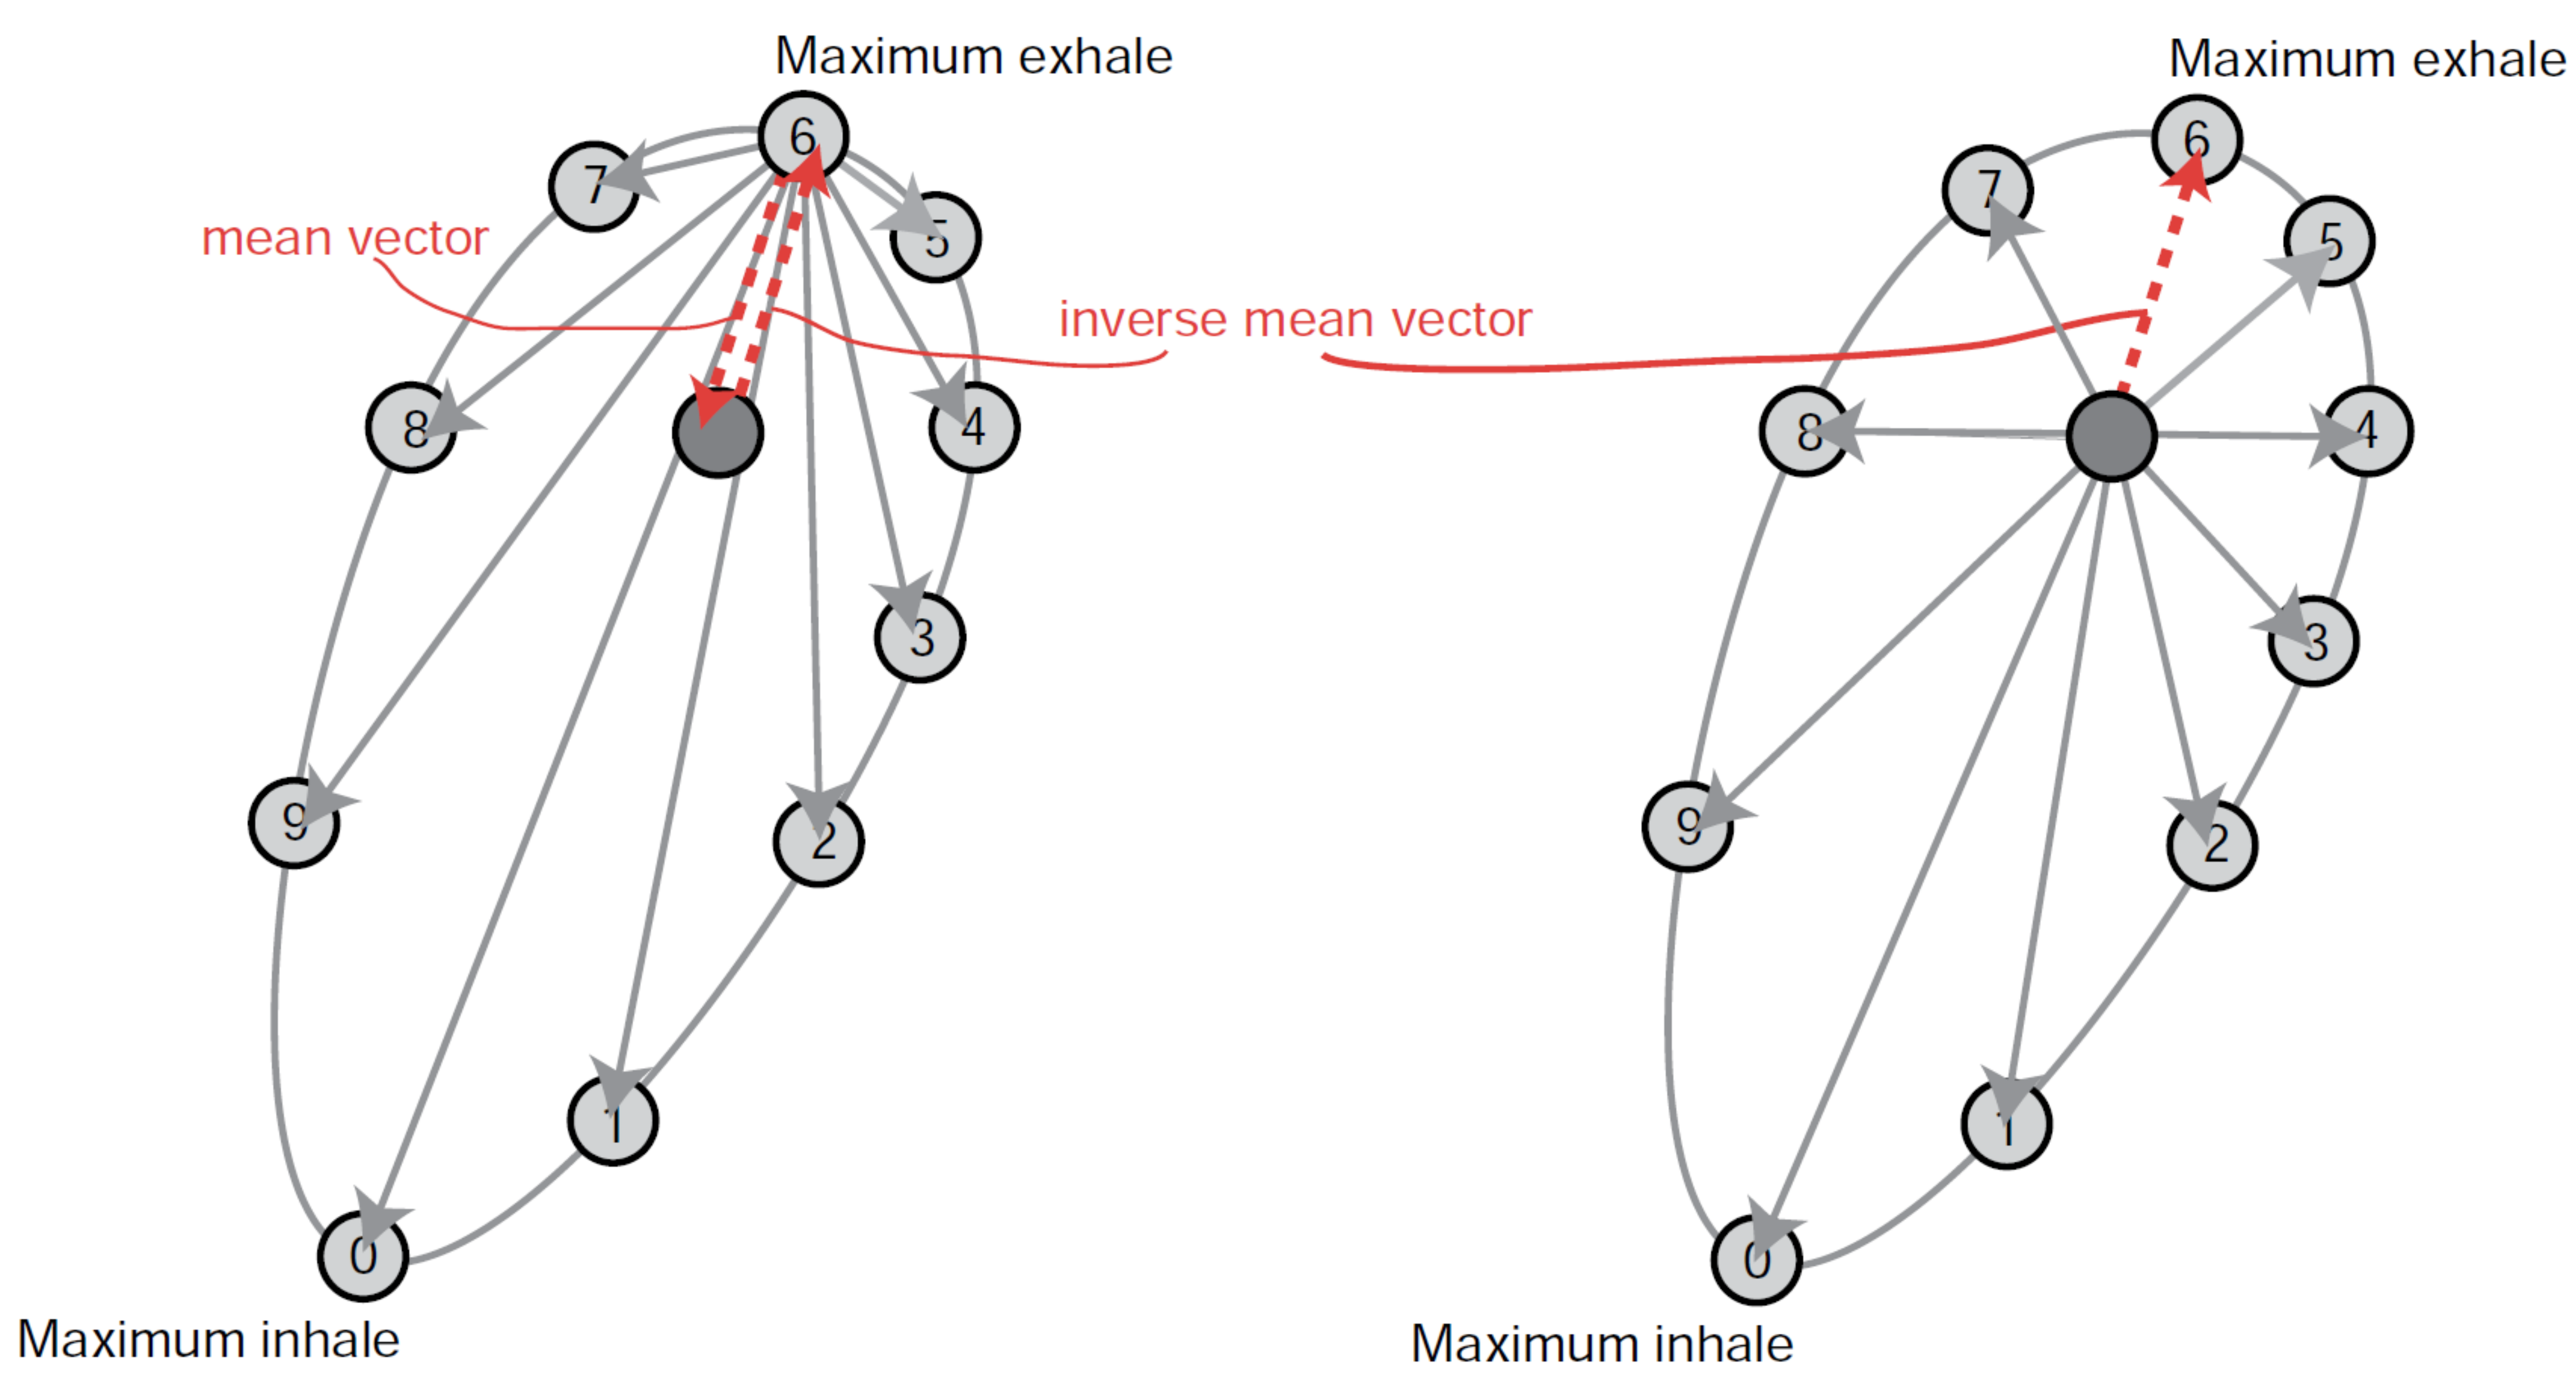
\includegraphics[width=0.9\textwidth]{./Vmm/Images/midPgeneration.png}
% \caption{Computation of the midP scan. All vectors have the same starting point (reference phase, maximum exhale in the this example), therefore they can be averaged, resulting in the mean vector.
% 	Next vectors from mean position to 4D-CT phases have to be computed, which is achieved by subtracting original vectors and mean vector. Figure taken from \cite{Wolthaus2008}}
% \label{midPgeneration}
% \end{center}
% \end{figure}


\newpage
\section{Verification}
\label{Verification}

Several tools to perform DIR and DIRQA were created. To prove their functionalities, we have tested them on two sets of an actual clinical data. 
First were the lung 4D-CT patient data from the Champalimaud Center for the Unknown, Lisbon (Portugal). The 4D-CTs were used in the treatment planning studies, presented in Chapters~\ref{PatStudy} and \ref{chapter:complex}. 
DIR resulting from 4D-CTs played an essential in these studies, since they were used in contour propagation to estimate and mitigate tumor motion. In addition, DIR was also used in 4D dose calculation.

The second set of data were pig cardiac 4D-CTs. They were also used in treatment planning as a part of an animal study, conducted at GSI. 
4D-CT DIR was also used for contour propagation and 4D dose calulation. However, the treatment plans were than actually used for the animal irradiation. It was therefore necessary not only to obtain DIR, but also to ensure its quality.

The DIRs were calculated as explained in Section~\ref{RegistrationImplement}. Afterwards absolute difference, Jacobian and ICE were calculated on resulting DIR as part of the the DIRQA. 

\subsection{Lung 4D-CT patient data}
\label{lungDIR}

The effects of interplay between tumor motion and active beam scanning can drastically change the dose distribution for PT. It is therefore necessary to estimate tumor motion and employ designated motion mitigation techniques.

Chapters \ref{PatStudy} and \ref{chapter:complex} present studies on simulating active scanning carbon ion treatment for non-small cell lung cancer patients.
The studies included data for 23 lung cancer patients. In order to calculate realistic treatment plans, 4D-CT scans were used in studies. 
All 4D-CT were registered to estimate and mitigate tumor motion and to calculate 4D doses. To ensure the DIR quality, DIRQA was performed on all DIRs.

\subsubsection{Materials and Methods}

In total, 23 lung cancer patients were studied. For each patient, a time-resolved CT (4D-CT) was acquired, consisting of 10 motion states (0 - 9) with 1 mm pixel and 1-2 mm slice spacing. 
They were acquired with either a Philips Brilliance BigBore 16-slice 
(Philips Healthcare, Eindhoven, Netherlands) or a Philips Gemini PET-CT 16-slice scanner. 
State 0 and 5 correspond to the end-inhale and end-exhale breathing state, respectively. State 0 was chosen as a reference state. 

True and inverse DIRs were computed for each patient between each state and the reference state. Each 4D-CT required 18 DIRs, leading to 414 DIRs in total.

The B-Spline Plastimatch module in Slicer was used for DIR (see Section~\ref{RegistrationImplement}). DIRs were done in two stages with details given in Table~\ref{tab:stages}. 

\begin{table}[H]
  \centering
%   \footnotesize
  \caption{Parameters used for B-Spline Plastimatch DIR. A mean squared error metric was used. Details for each parameter can be found in \cite{Plastimatch}.}
  \begin{tabular}{c|c|c}
      Parameter & Stage 1 & Stage 2 \\
      \hline
      Resolution & 4,4,2 & 1,1,1 \\
      Grid size & 50 & 15 \\
      Regularization lambda & 0.005 & 0.005 \\
      Iterations & 200 & 100 \\
    \hline\hline
  \end{tabular}
  \label{tab:stages}
\end{table}


A box-shaped ROI around the patient body was created with a Slicer build-in function. The ROI was employed in calculation of absolute difference, Jacobian and ICE.

Default, true and inverse absolute difference were calculated. In total 621 absolute differences were calculated. All images were down-sampled by a factor of 2
before calculation of absolute difference to save computer time. Similarly, 414 vector fields were down-sampled by a factor of 2 before calculating Jacobian and ICE. Jacobian and ICE checks were calculated on all vector fields.
Additionally, vector field magnitudes were analyzed for mean, standard deviation (STD) and maximum (max) values. Paired t-tests were performed to compare mean, STD and max of true and inverse vector field magnitudes.
A p-value < 0.05 was considered significant. A Pearson's r coefficient was used to determine linear fit quality.


For each patient it took around 20 min for all 18 DIRs and around 30 min for complete DIRQA on the 9 motion states. A cluster of different Linux computers, each with 8 CPU and 32 GB RAM were used for DIR and DIRQA.

DIR was used in treatment planning, specifically in contour propagation and 4D dose calculation. The areas with poor DIR were investigated and distance between DIR errors 
and target contour was measured. If the target and the beam path was more than 5 cm away from DIR errors, DIR was not repeated.

\newpage

\begin{figure}[H]
	\begin{center}		
		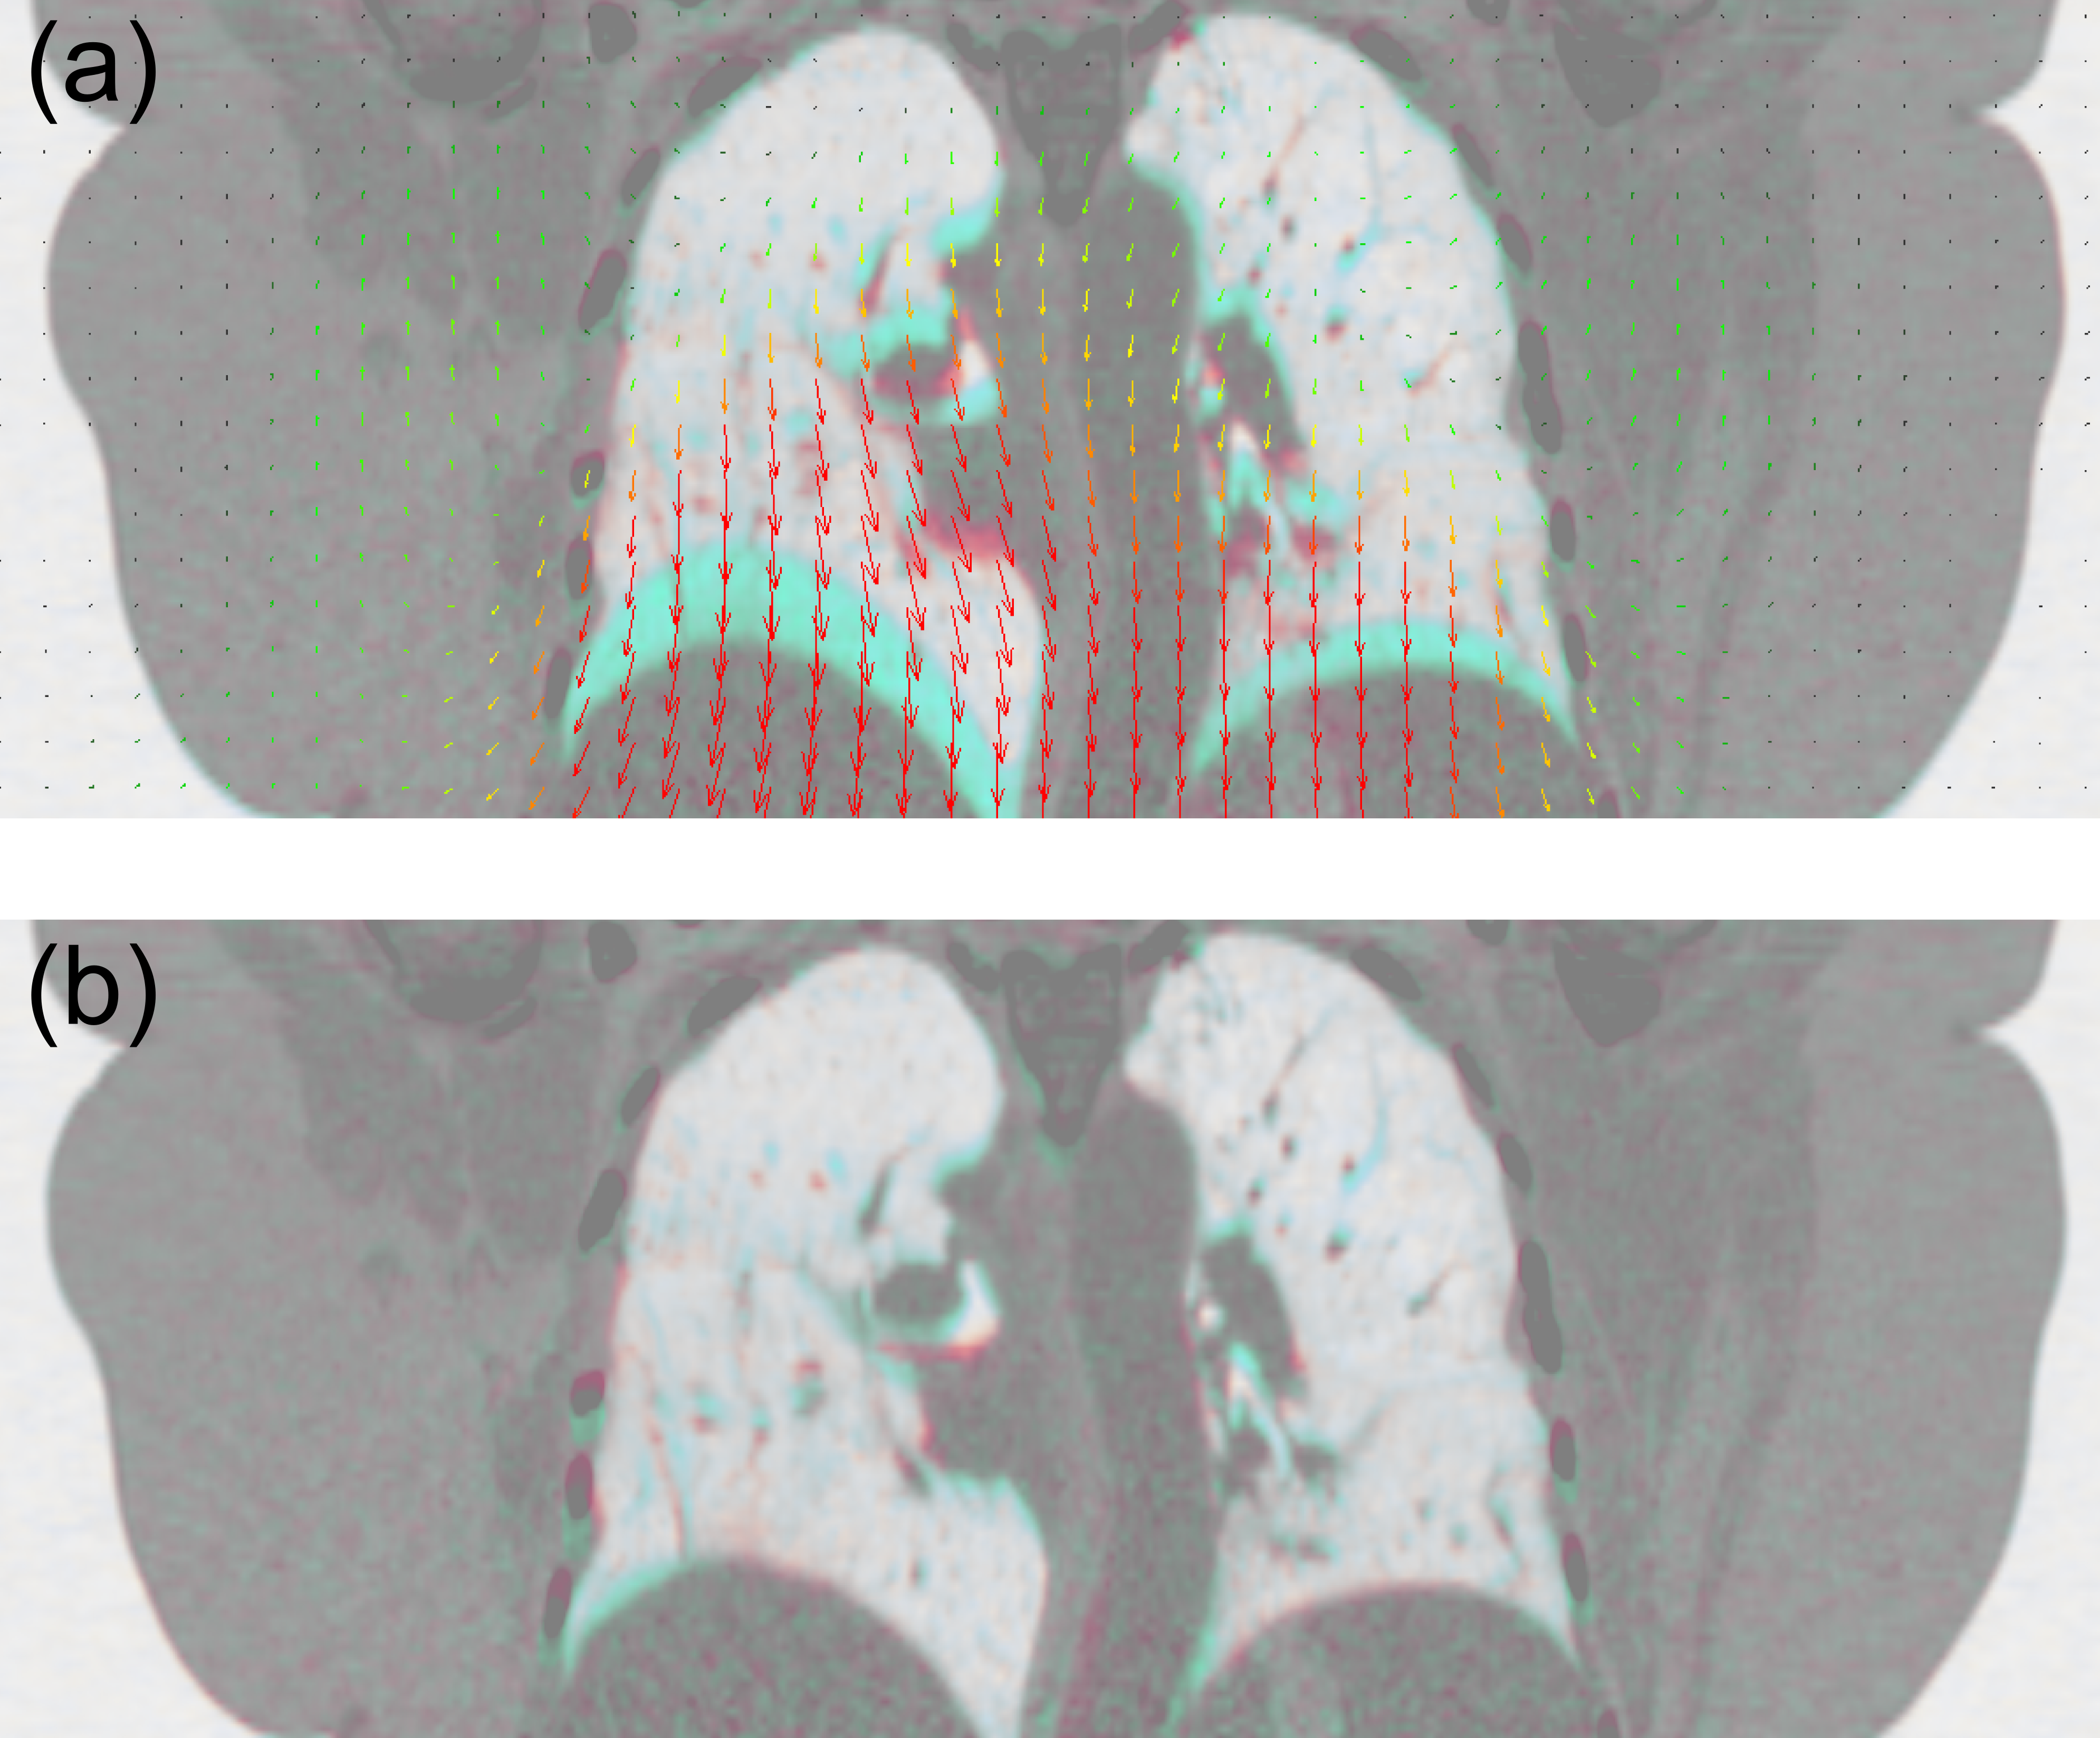
\includegraphics[width=0.6\textwidth]{./Vmm/Images/exampleReg.png}
		\caption{Inverse color overlay of two states before (a) and after (b) DIR. Vector field is displayed on image (a) as arrows.}
		\label{exampleReg_lung}
	\end{center}
\end{figure}


\subsubsection{Results}

An example of a DIR is displayed in Fig.~\ref{exampleReg_lung}. The statistical analysis of vector fields is shown in Table~\ref{tab:vectordata_lung}. No statistical
difference between true and inverse vector field magnitudes was found. The biggest contribution to vector field magnitude was from superior-inferior direction (around 50\%), followed by anterior-posterior direction (around 30\%)
by left-right direction (around 20\%).

\begin{table}[H]
  \centering
%   \footnotesize
  \caption{Data of vector magnitudes. Values are presented as mean (range).}
  \begin{tabular}{c|c|c}
  
       & True vector field (mm) & Inverse vector field (mm) \\
       \hline
       Mean & 0.38 (0.01 - 1.28) & 0.38 (0.01 - 1.3) \\ 
       STD & 0.95 (0.04 - 3.17) & 0.98 (0.04 - 3.55) \\ 
       Max & 9.67 (0.61 - 28.56) & 10.17 (0.56 - 37.11) \\
    \hline\hline
  \end{tabular}
  \label{tab:vectordata_lung}
\end{table}

The correlation between absolute difference before (default) and after DIR (true and inverse) is shown in Fig.~\ref{absDiff_lung}. It also shows default absolute difference distribution across 9 states. 

Distribution of true and inverse Jacobian and ICE data are displayed in Fig. \ref{jacobian_data}. 

True and inverse maximum and minimum Jacobian and maximum ICE values were plotted against maximum vector magnitudes and fitted with linear function. The results are shown in Fig.~\ref{maxvf}.


Linear fits used in Fig.~\ref{absDiff_lung} and ~\ref{maxvf} were statistically significant (p < 0.05).

All areas with poor DIR were further than 5 cm away from the target and no repetition of DIR was necessary.

\begin{figure}[H]
	\begin{center}		
		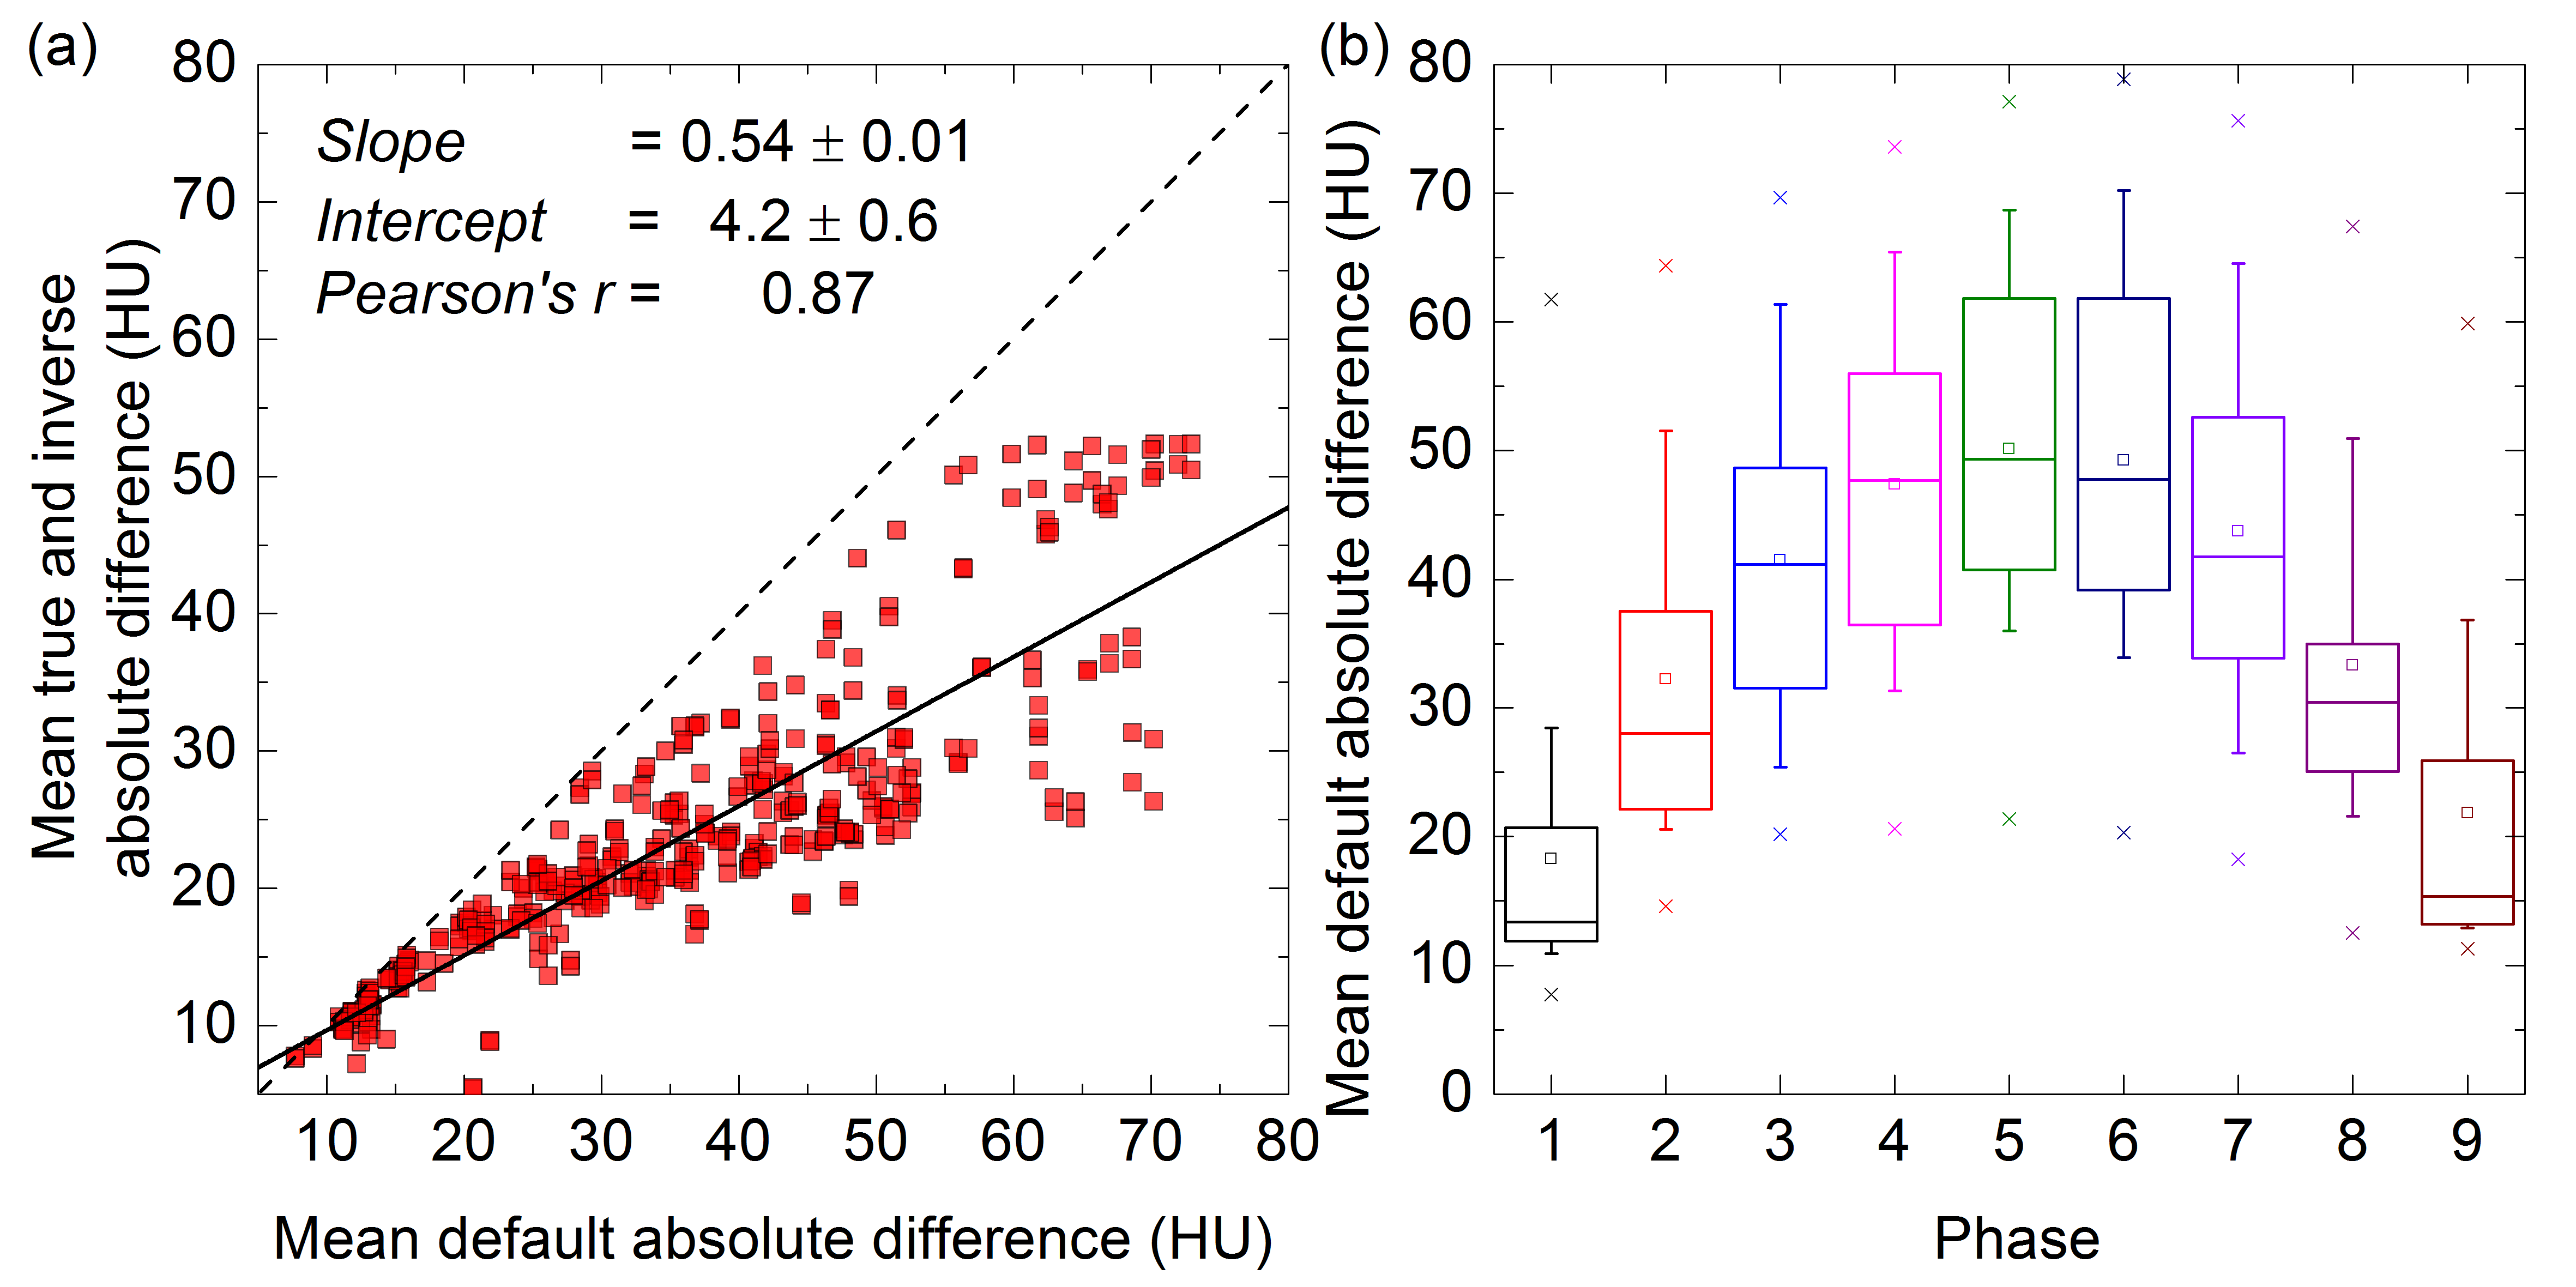
\includegraphics[width=0.7\textwidth]{./Vmm/Images/absDiff.png}
		\caption{(a) The mean true and inverse absolute difference plotted against the mean default absolute difference. The solid line shows a linear fit, with parameters
		written in the top left corner. Dashed line shows $y(x)=x$. (b) Box plots of mean default absolute difference distribution across nine 4D-CT states. Boxes represent 25-75\%, whiskers 10-90\%
		of data. The median is shown with a solid line, the mean is represented with squares and outliers with crosses.}
		\label{absDiff_lung}
	\end{center}
\end{figure}

\newpage

\begin{figure}[H]
	\begin{center}		
		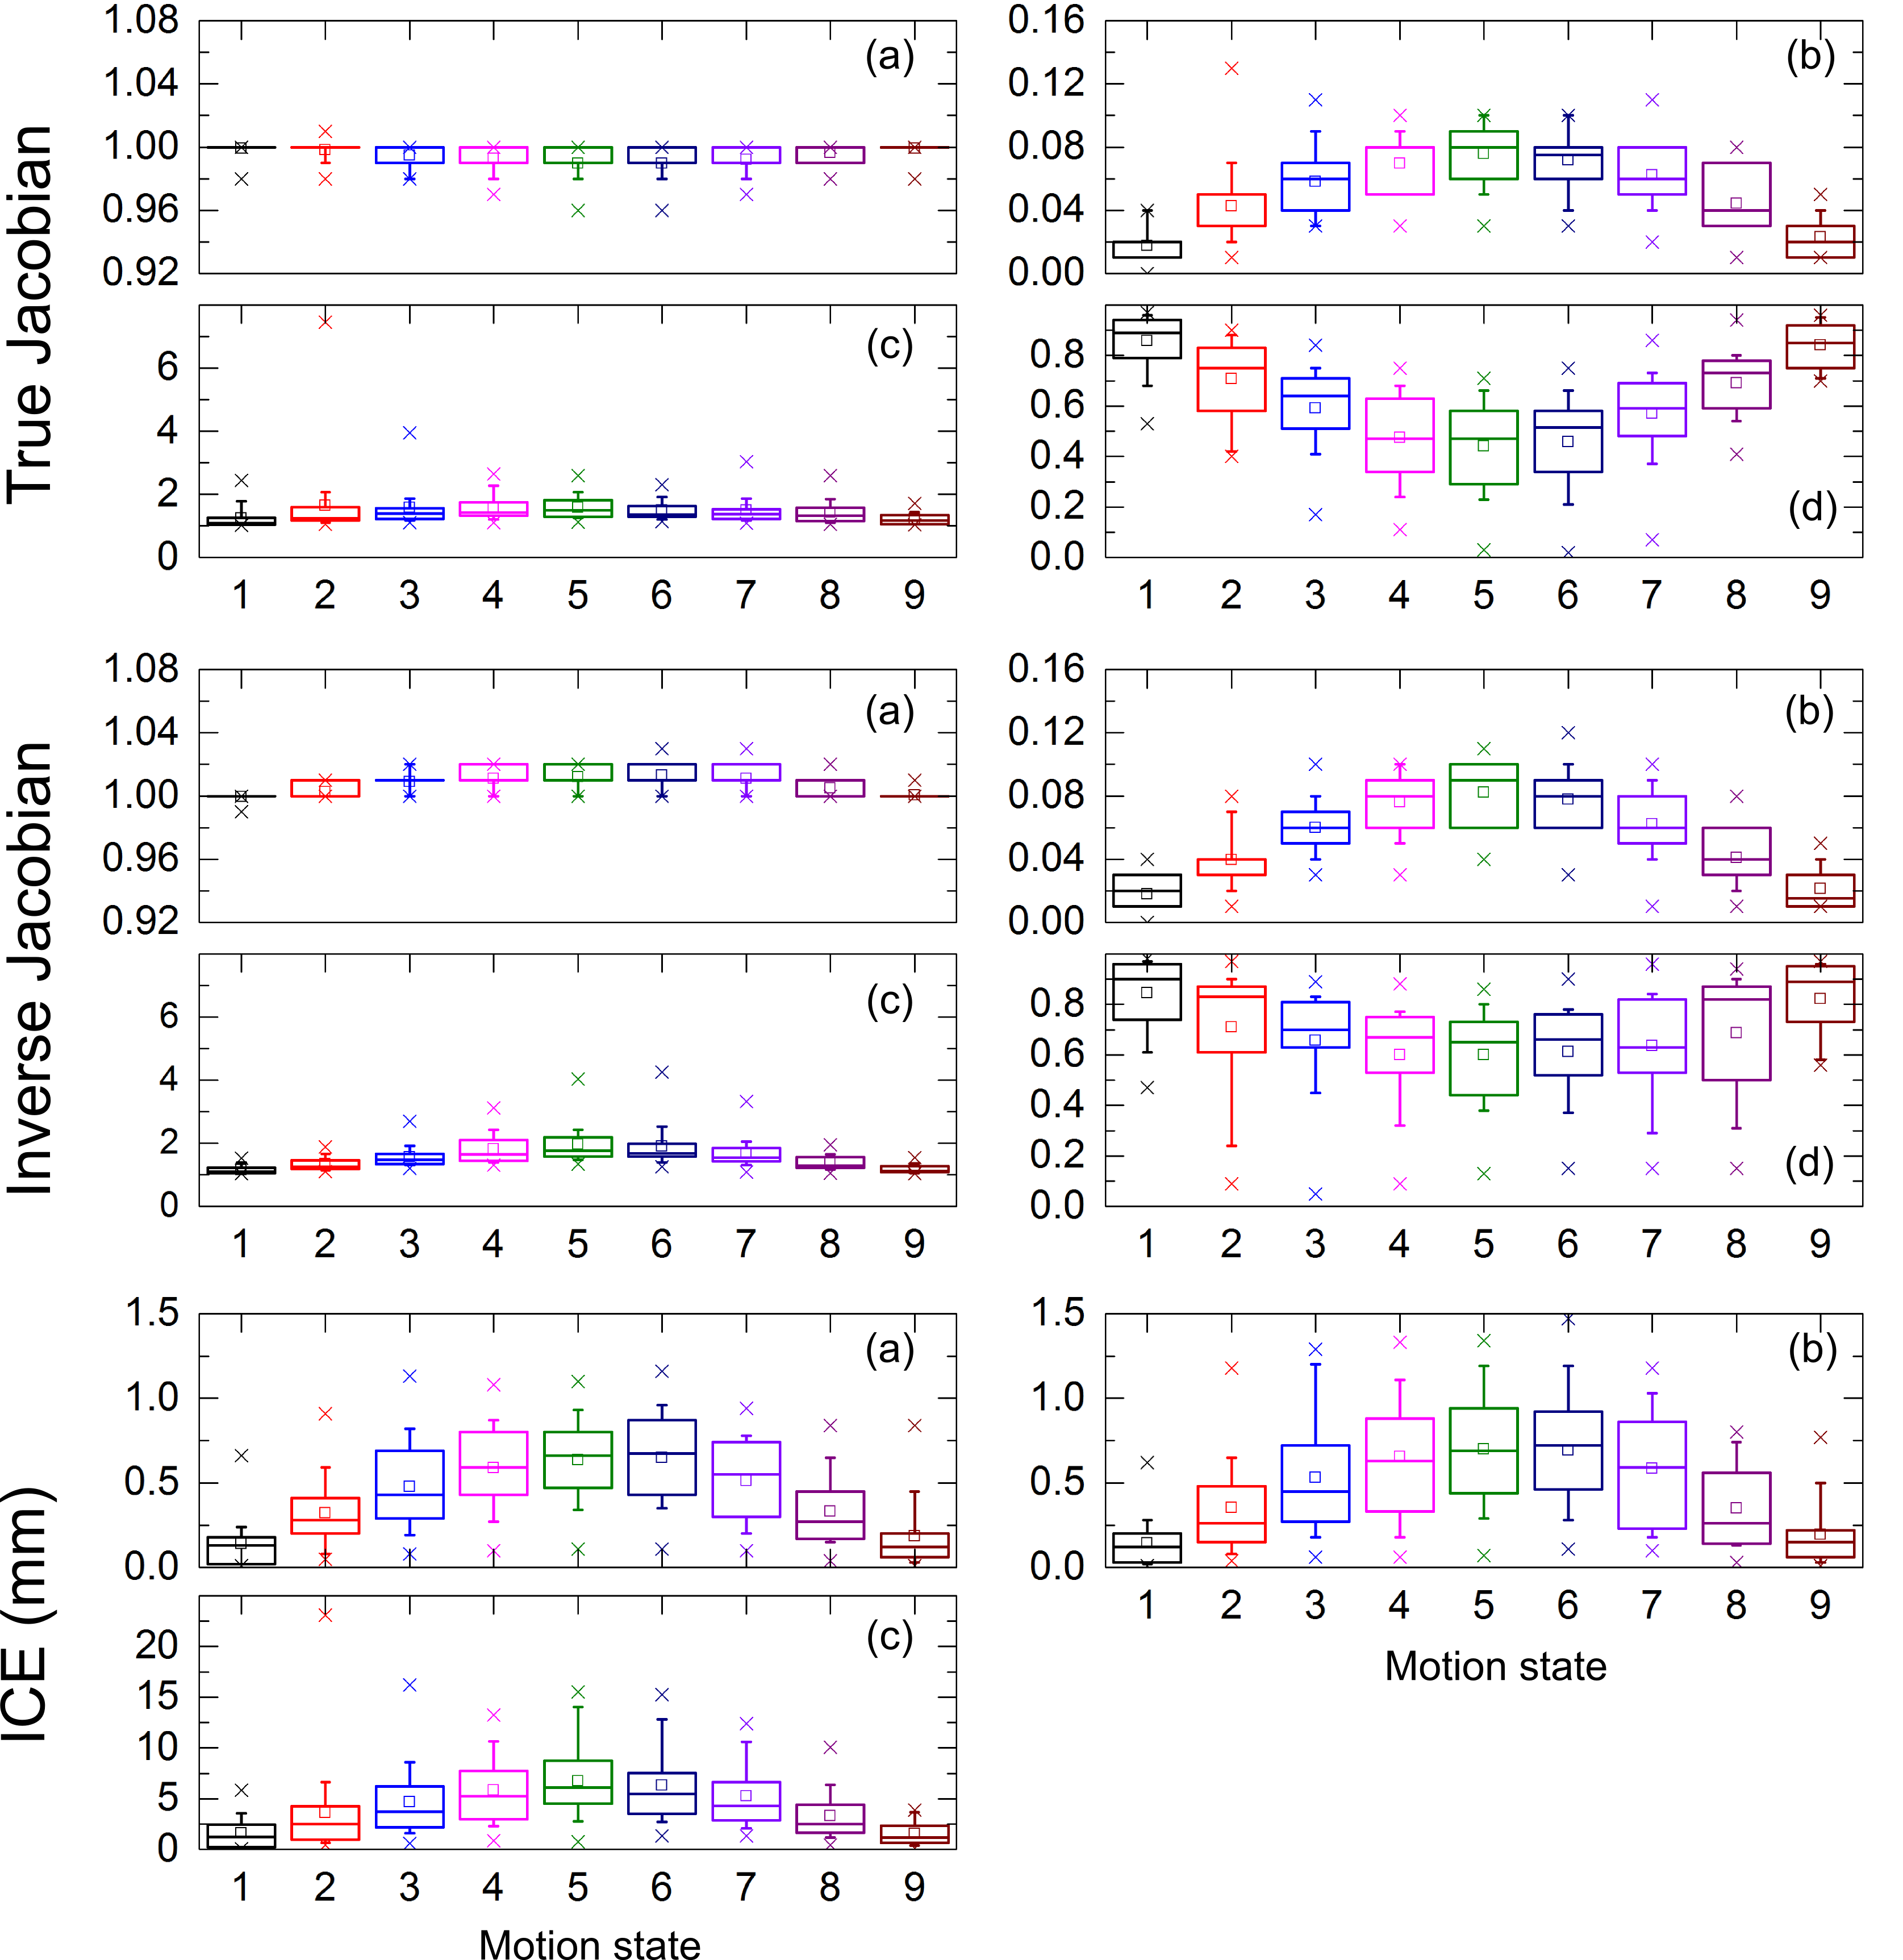
\includegraphics[width=0.9\textwidth]{./Vmm/Images/Jacobian_data.png}
		\caption{Data for the true (top) and inverse (middle) Jacobian and ICE (bottom) for 9 4D-CT states (reference state 0 is excluded) for 23 lung cancer patients. Mean, STD, maximum and minimum are represented as (a), (b), (c) and (d), respectively.
		Minimum ICE is 0 throughout all states and patients. Boxes represent 25-75\%, whiskers 10-90\%
		of data. The median is shown with a solid line, the mean is represented with squares and outliers with crosses.}
		\label{jacobian_data}
	\end{center}
\end{figure}

\newpage

% \begin{figure}[H]
% 	\begin{center}		
% 		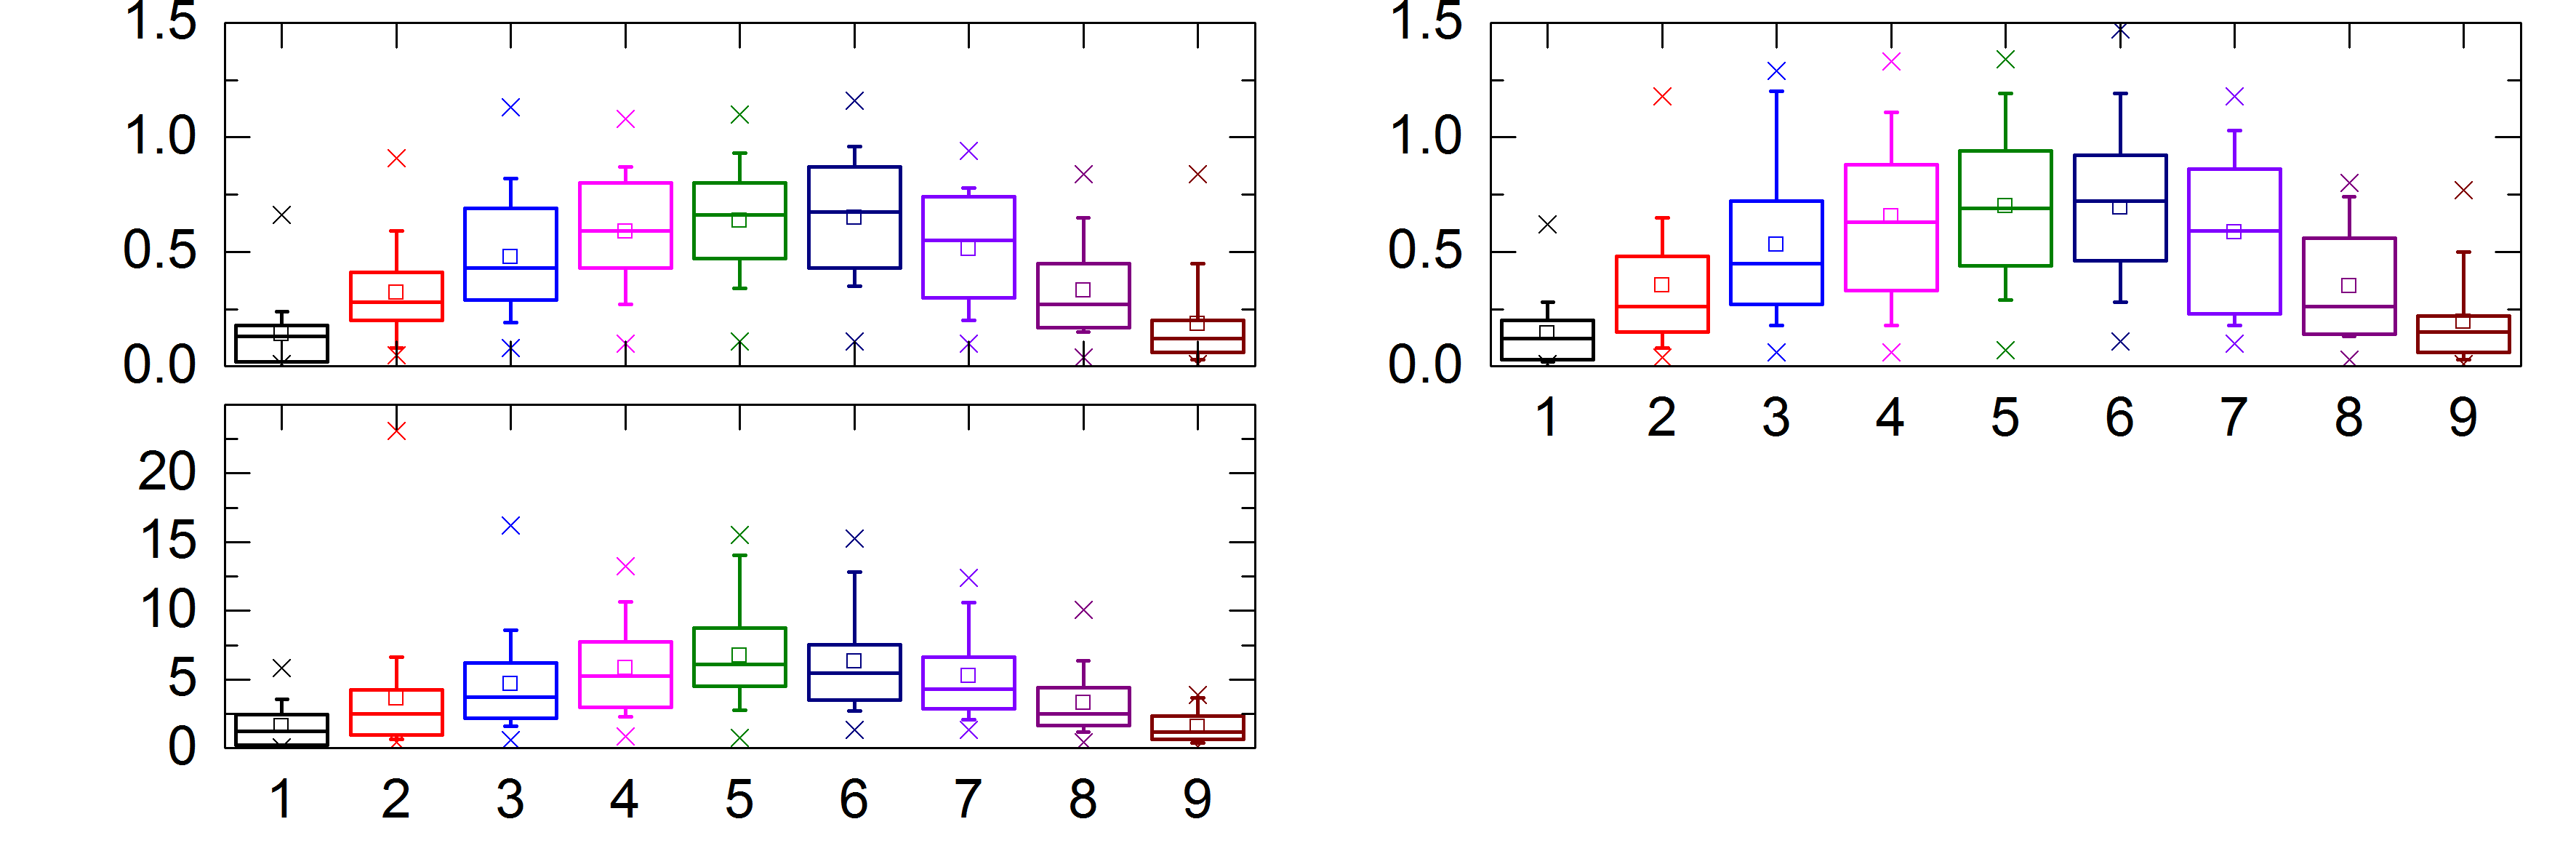
\includegraphics[width=0.9\textwidth]{./Vmm/Images/ICE.png}
% 		\caption{Data for ICE for 9 4D-CT states (reference state 0 is excluded) for 23 lung cancer patients. Mean, STD, maximum are represented as (a), (b) and (c), respectively. ICE Minimum is 0 throughout all states and patients.
% 		Boxes represent 25-75\%, whiskers 10-90\% of data, median is shown with a solid line, mean with squares and outliers with crosses.}
% 		\label{ice}
% 	\end{center}
% \end{figure}



% \begin{figure}[H]
% 	\begin{center}		
% 		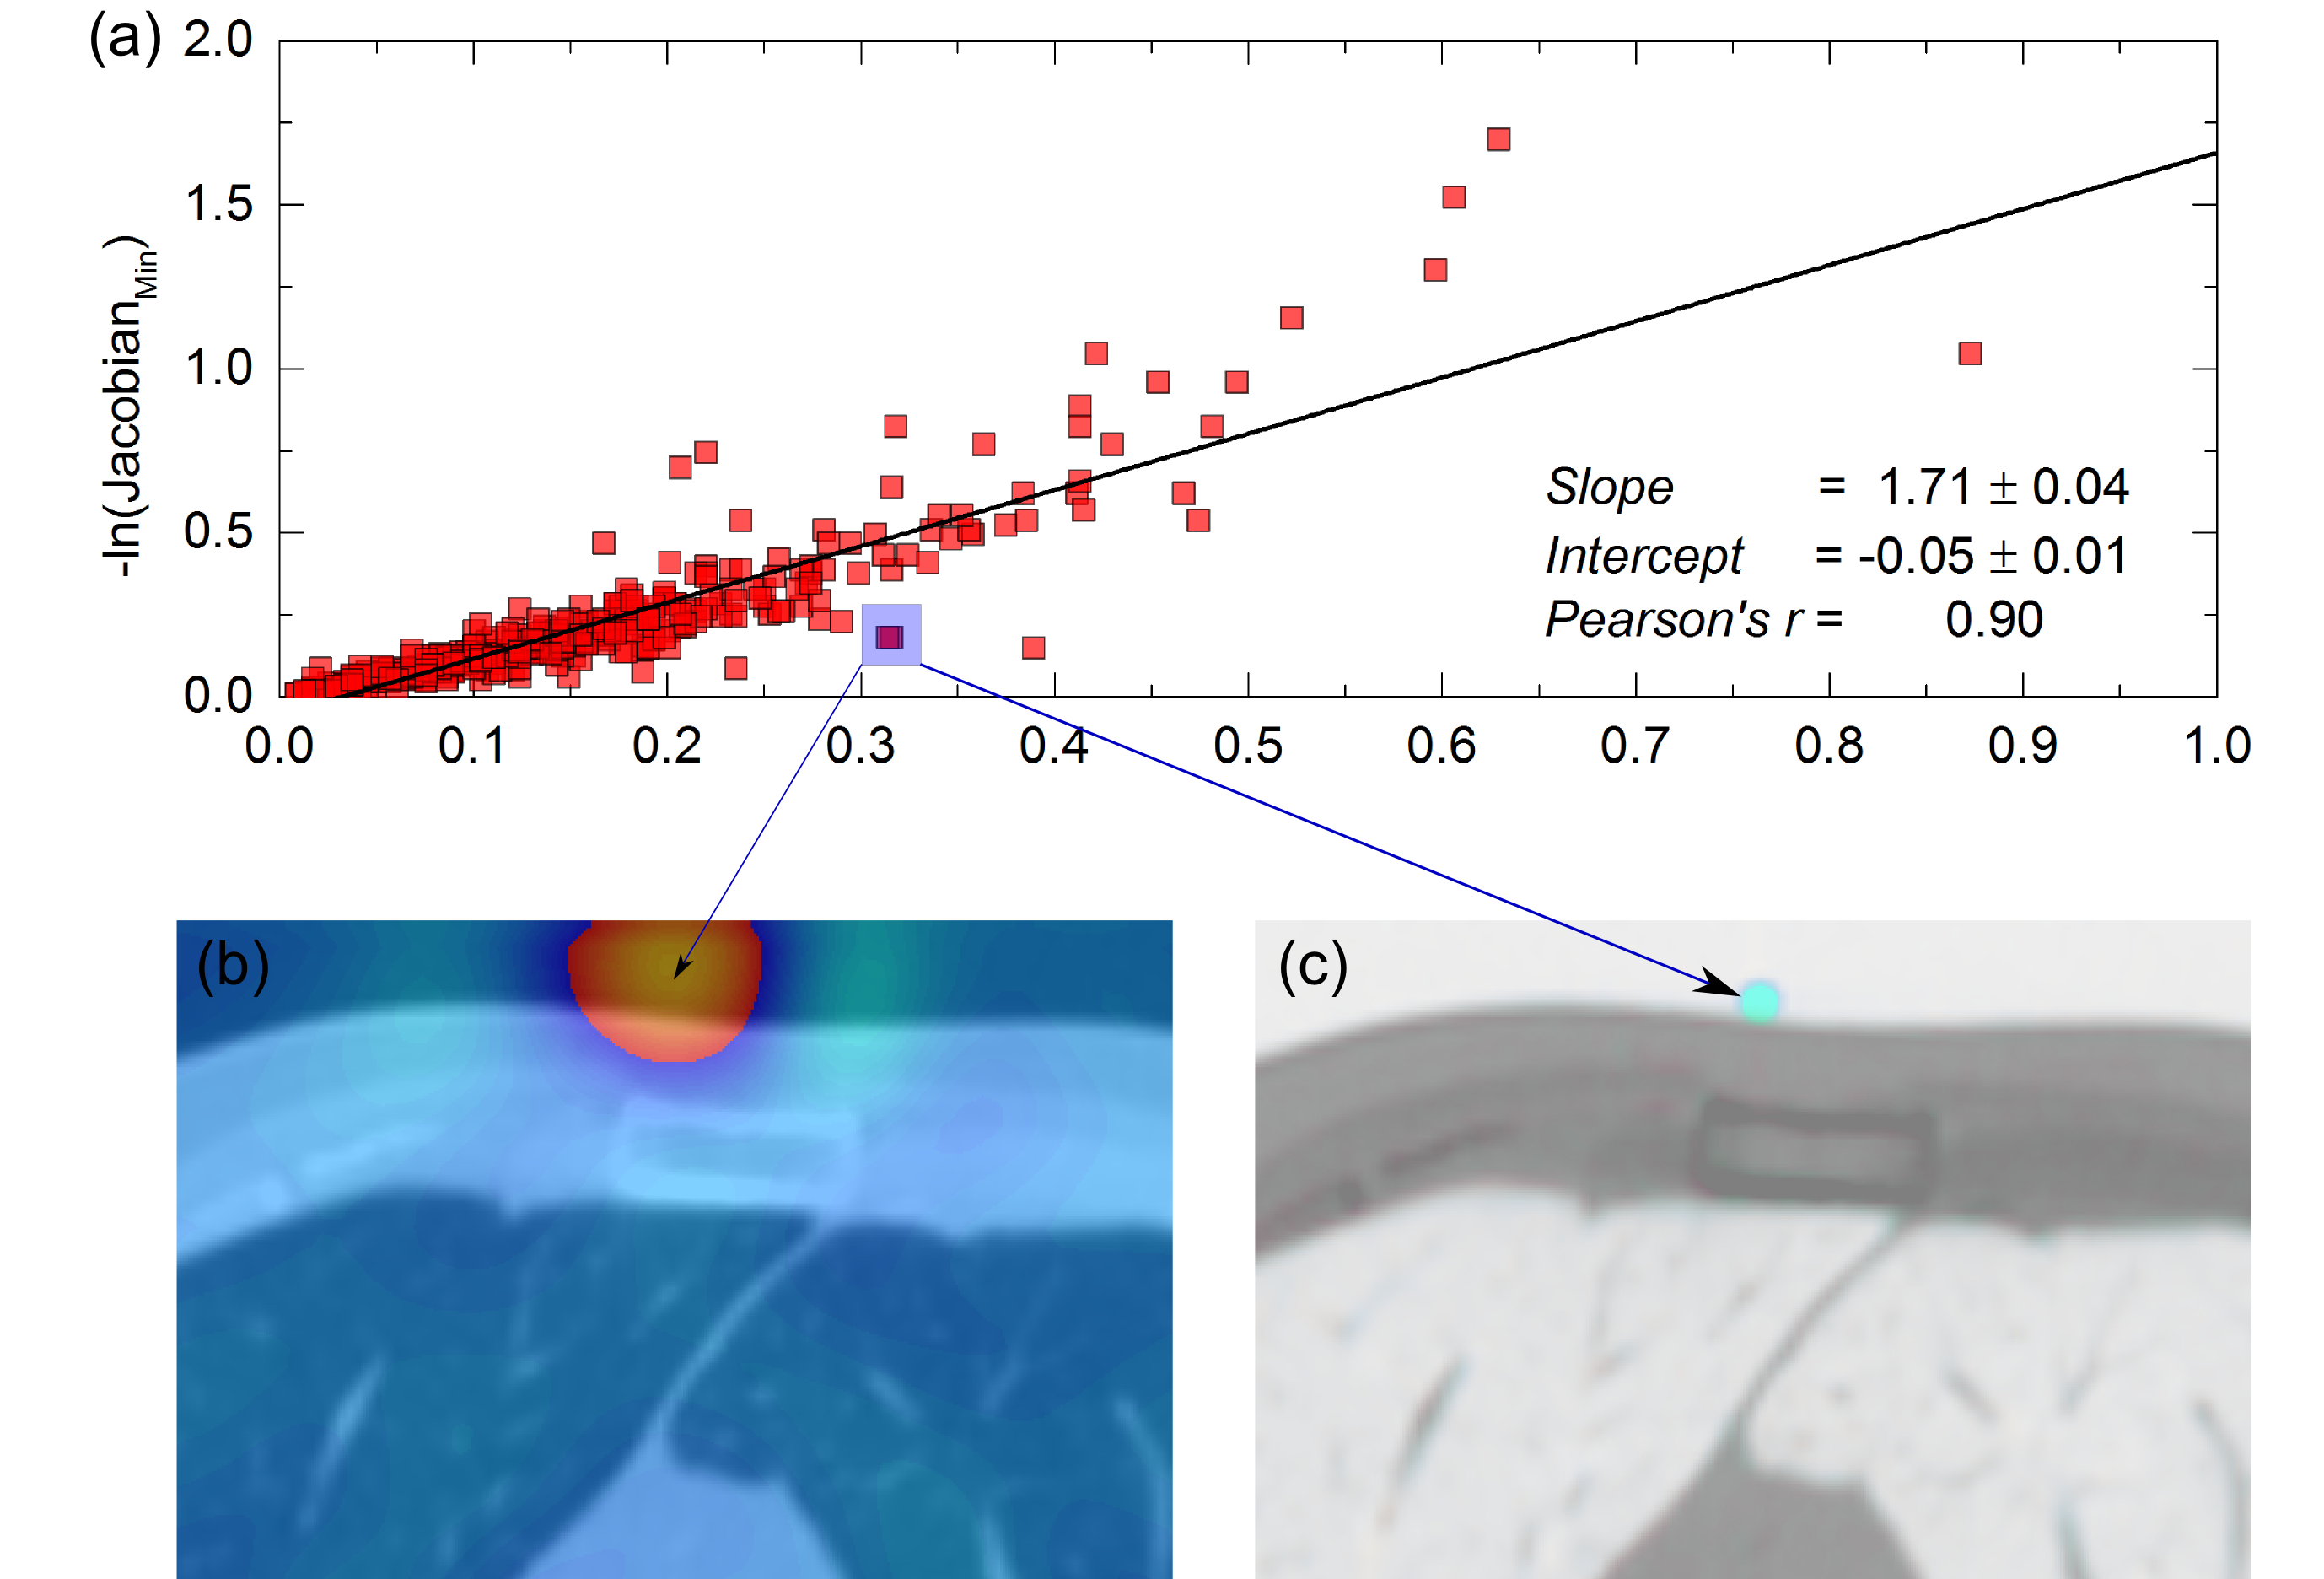
\includegraphics[width=0.8\textwidth]{./Vmm/Images/jacSum_lung.png}
% 		\caption{(a) Plot of negative natural logarithm of minimum inverse (true) Jacobian versus natural logarithm of maximum true (inverse) Jacobian. Linear fit is displayed with solid line and it's parameters are given in the corner. A deviation from linear fit (highlighted with blue square)
% 			was used as an example of scaled Jacobian (see text), shown in (b). (c) shows the CT the states highlighted in (a) in inverse color, where an artifact is clearly seen in one state and not the other.}
% 		\label{calcJac_lung}
% 	\end{center}
% \end{figure}

\newpage

\begin{figure}[H]
	\begin{center}		
		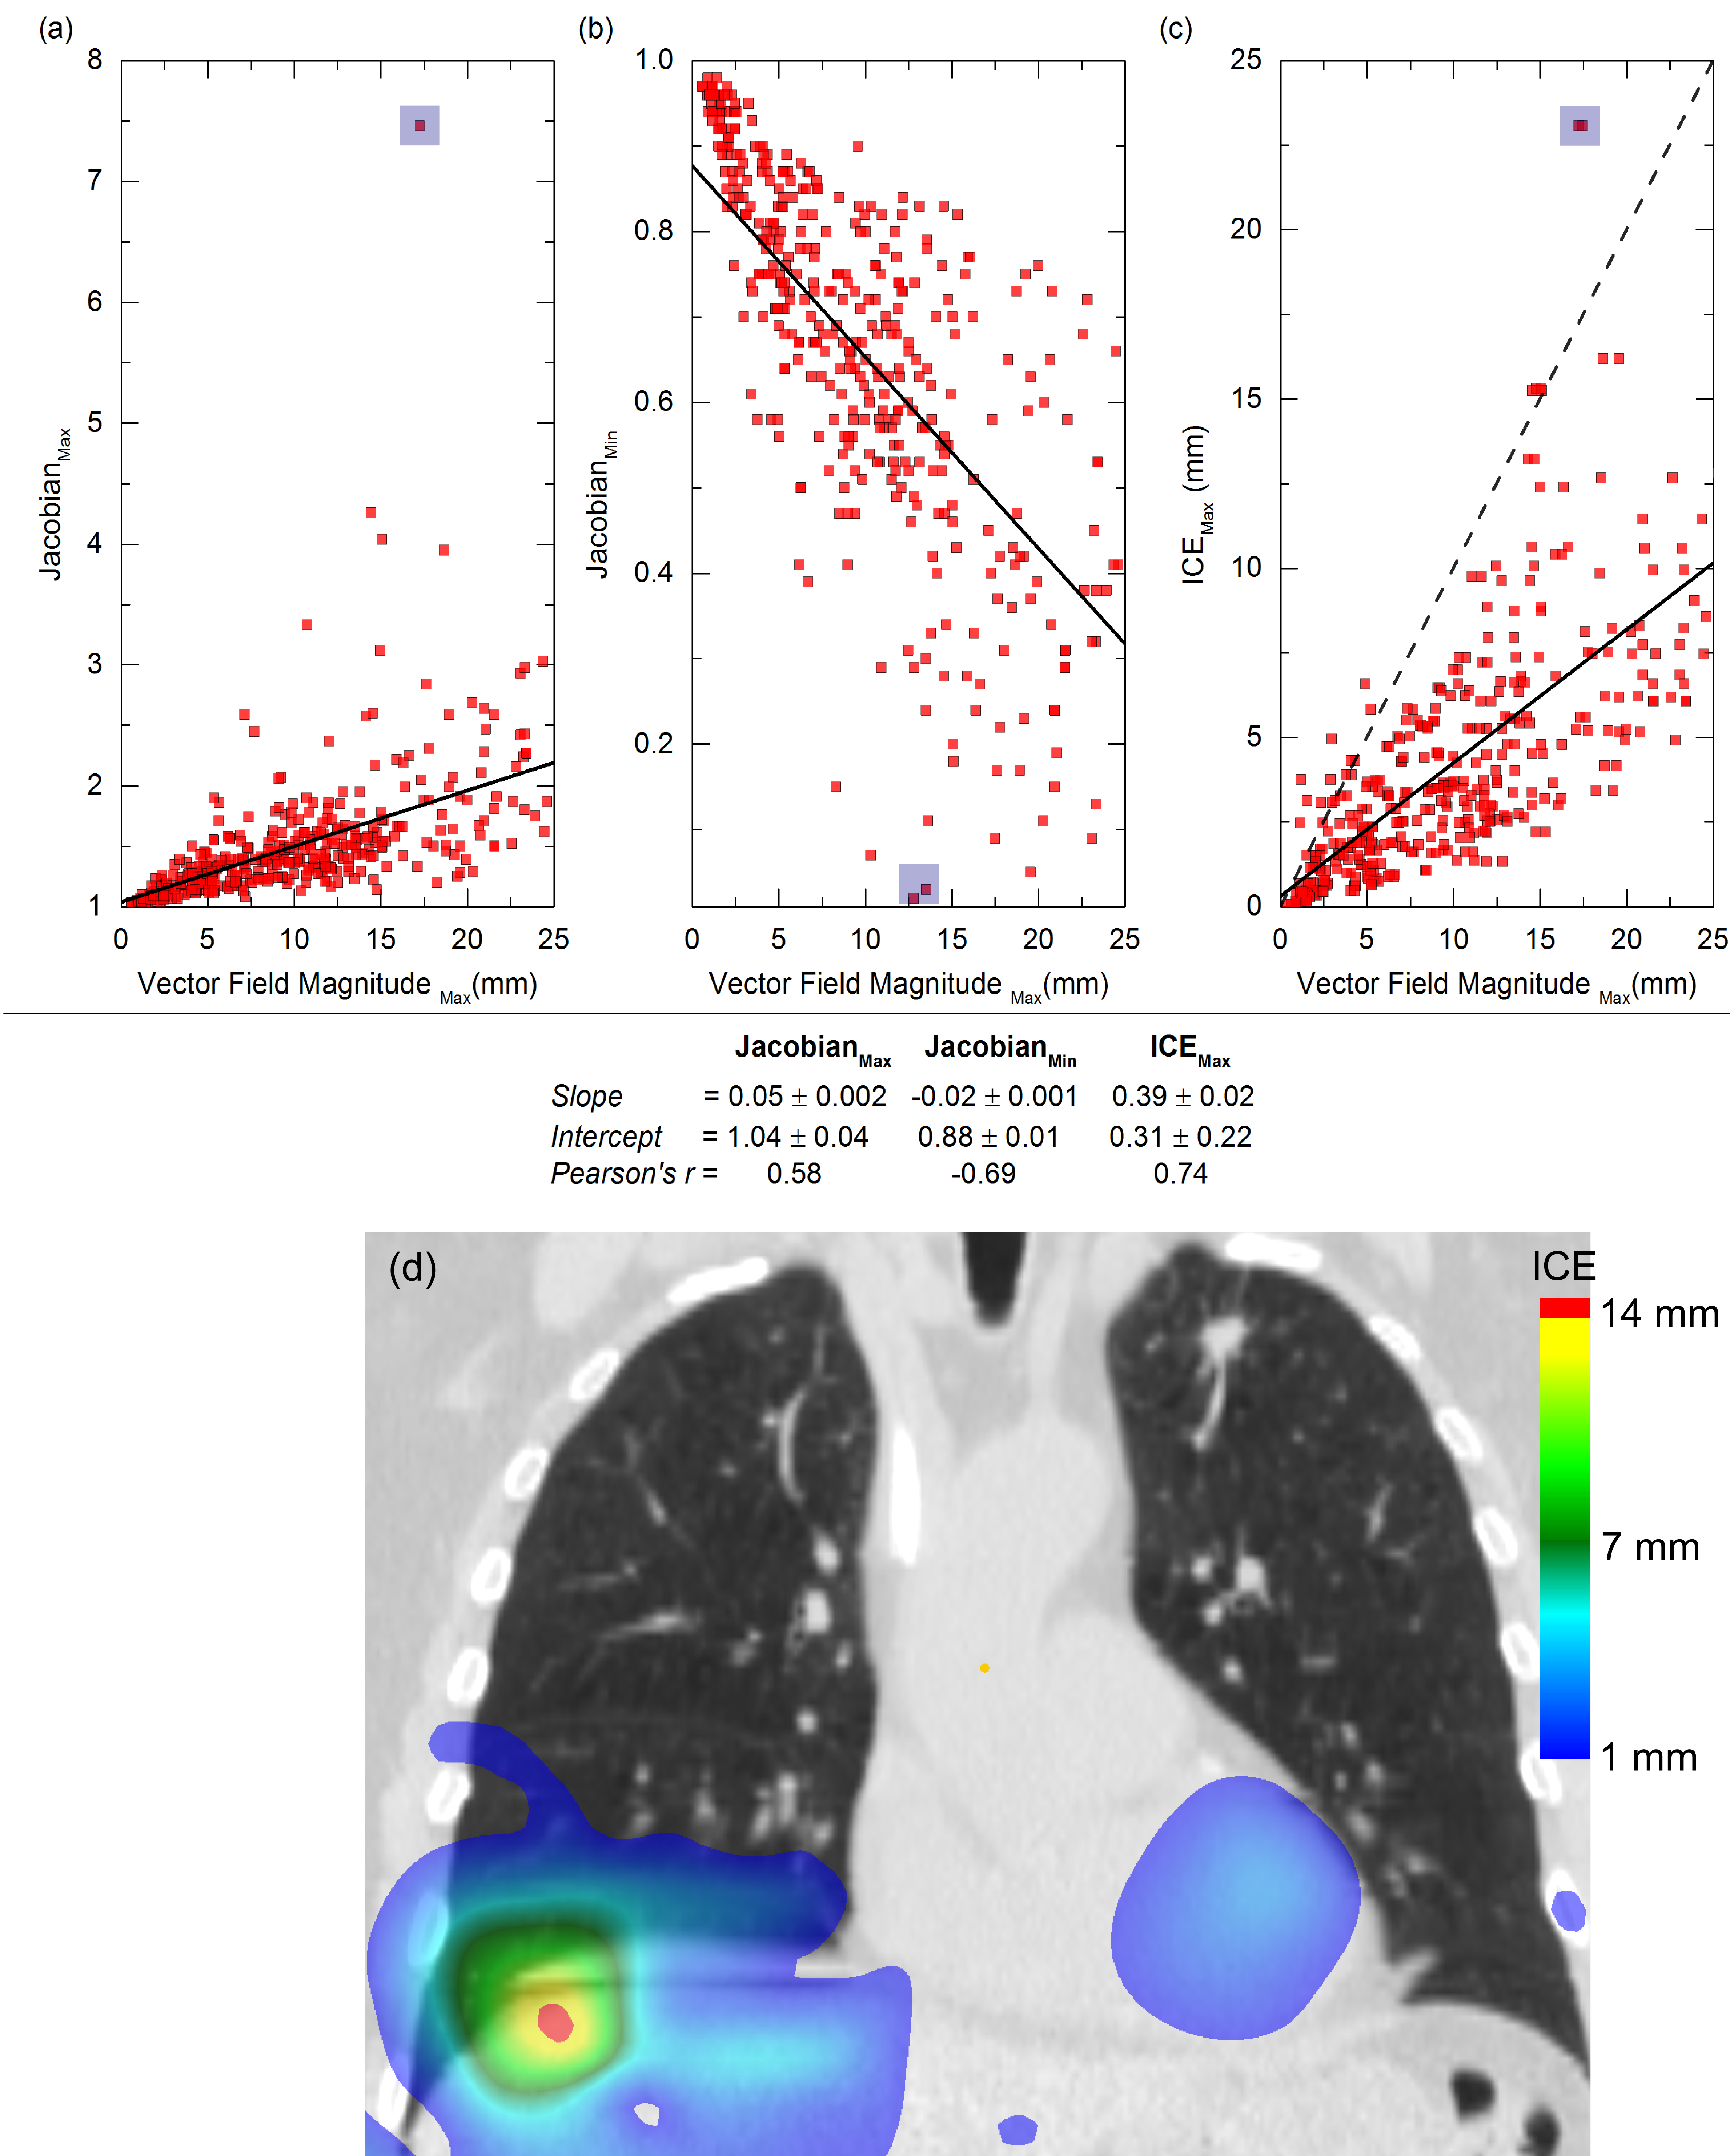
\includegraphics[width=0.9\textwidth]{./Vmm/Images/maxVf_lung.png}
		\caption{Values of maximum Jacobian (a), minimum Jacobian (b) and maximum ICE (c) plotted against the maximum vector magnitudes. A linear fit is displayed with a solid line and parameters are written below the plots. 
		The dashed line in (c) shows $y(x)= x$ plot.
			The points highlighted with blue squares come from the same DIR error that is shown in Fig.~\ref{contourPropagation}}
		\label{maxvf}
	\end{center}
\end{figure}

\newpage
\subsubsection{Discussion}

Nine states of 4D-CTs were registered to a 4D-CT reference state for 23 lung cancer patients, producing 414 true and inverse vector fields. 
All 414 DIR underwent a DIRQA consisting of vector field magnitudes, absolute difference, Jacobian and ICE.

Vector field magnitudes confirm previously published data that the biggest motion for lungs is in superior-inferior direction \cite{Seppenwoolde2002, Britton2007, Liu2007}. The mean vector field magnitude is small (in submilimeter range), 
because the ROI included the whole patient body, not just the lungs where most of the motion occurs. Vectors and inverse vectors are similar, which was expected.

There was a high correlation (Pearson's r = 0.87) between absolute difference before and after DIR. 
The slope of the linear fit suggests that the B-Spline DIR on average halves the absolute difference. There are several outliers from the
linear fit for default absolute difference bigger than 50 HU, however no DIR errors could be found upon visual inspection for this outliers.
All absolute differences after the DIR are smaller then before, which is a necessary condition in order for DIR to be considered successful. Apart from smaller absolute difference after DIR,
nothing could be deducted about the DIR quality from the absolute difference. The absolute difference is limited by the
image noise, which will always be present in a CT scan \cite{Polacin1992}. It would be interesting to study the 
correlation between image noise, absolute difference and consequential DIR quality.


Due to small mean vector field magnitudes, average values for true and inverse Jacobian were $1\pm0.05$, which indicates that most of the patient body does not change during the 4D-CT
scan. However, patients expansions and contractions can be seen on maximum and minimum Jacobian, with average values around 1.50 and 0.65 respectively. 
% If a part of a patient body contracts from reference to moving image, 
% then it expands in inverse direction and vice versa. The correlation was confirmed in Fig.~\ref{calcJac_lung}a, with a high Pearson's r (0.90). Furthermore outliers from linear fit spot inconsistencies
% in DIR as shown in Fig.~\ref{calcJac_lung}b and c, where a small artifact was found in one patient state solely from the deviation from linear fit in Fig.~\ref{calcJac_lung}. A scaled Jacobian could be used as a DIRQA check.

ICE Mean and STD values were in submilimeter range, due to the correlation between vector field and ICE (see Eq.~\ref{eq:ice}). The maximum ICE (2.3 cm) was observed in a patient with 
an artifact present in state 2 of the 4D-CT, as shown in Fig.~\ref{maxvf}.
% but still smaller as average maximum vector values. 

Large vector field magnitudes will produce more errors in DIR as shown in Fig~\ref{maxvf}. Linear fits were used to estimate the increase (decrease) of the Jacobian and ICE. 
As a rough DIRQA check, ICE should always be smaller than the maximum vector field magnitude. To confirm this, all cases above the dashed line in Fig~\ref{maxvf}c 
were investigated. For all areas of poor DIR were found. An extreme case (highlighted in Fig.~\ref{maxvf}a-c)
had a large image artifact present in states 2 and 3 (state 3 with ICE is shown in Fig.~\ref{maxvf}d) leading to large inconsistencies in DIR. 
The effect of DIR inconsistency on contour propagation can be seen in Fig.~\ref{contourPropagation},
where lungs and liver contour were propagated using DIR. The propagated contours clearly differ from the image features.

The 4D-CT DIRs investigated here were used in particle therapy treatment planning. All areas that were found to have a poor DIR, were so far away from the target, that contour propagation or 4D dose calculation were not affected.
Hence a repetition of DIR was not necessary.
The patient in Fig.~\ref{contourPropagation}a had a tumor in the upper left lung lobe and DIR inconsistencies were found in lower right lung lobe, as can be seen in Fig~\ref{contourPropagation}b. 
Therefore all DIRs were considered as successful. 
% It should be stressed, however, that in this study only 4D-CTs that had a good contrast and no image artifacts in tumor vicinity were used.

\begin{figure}[H]
	\begin{center}		
		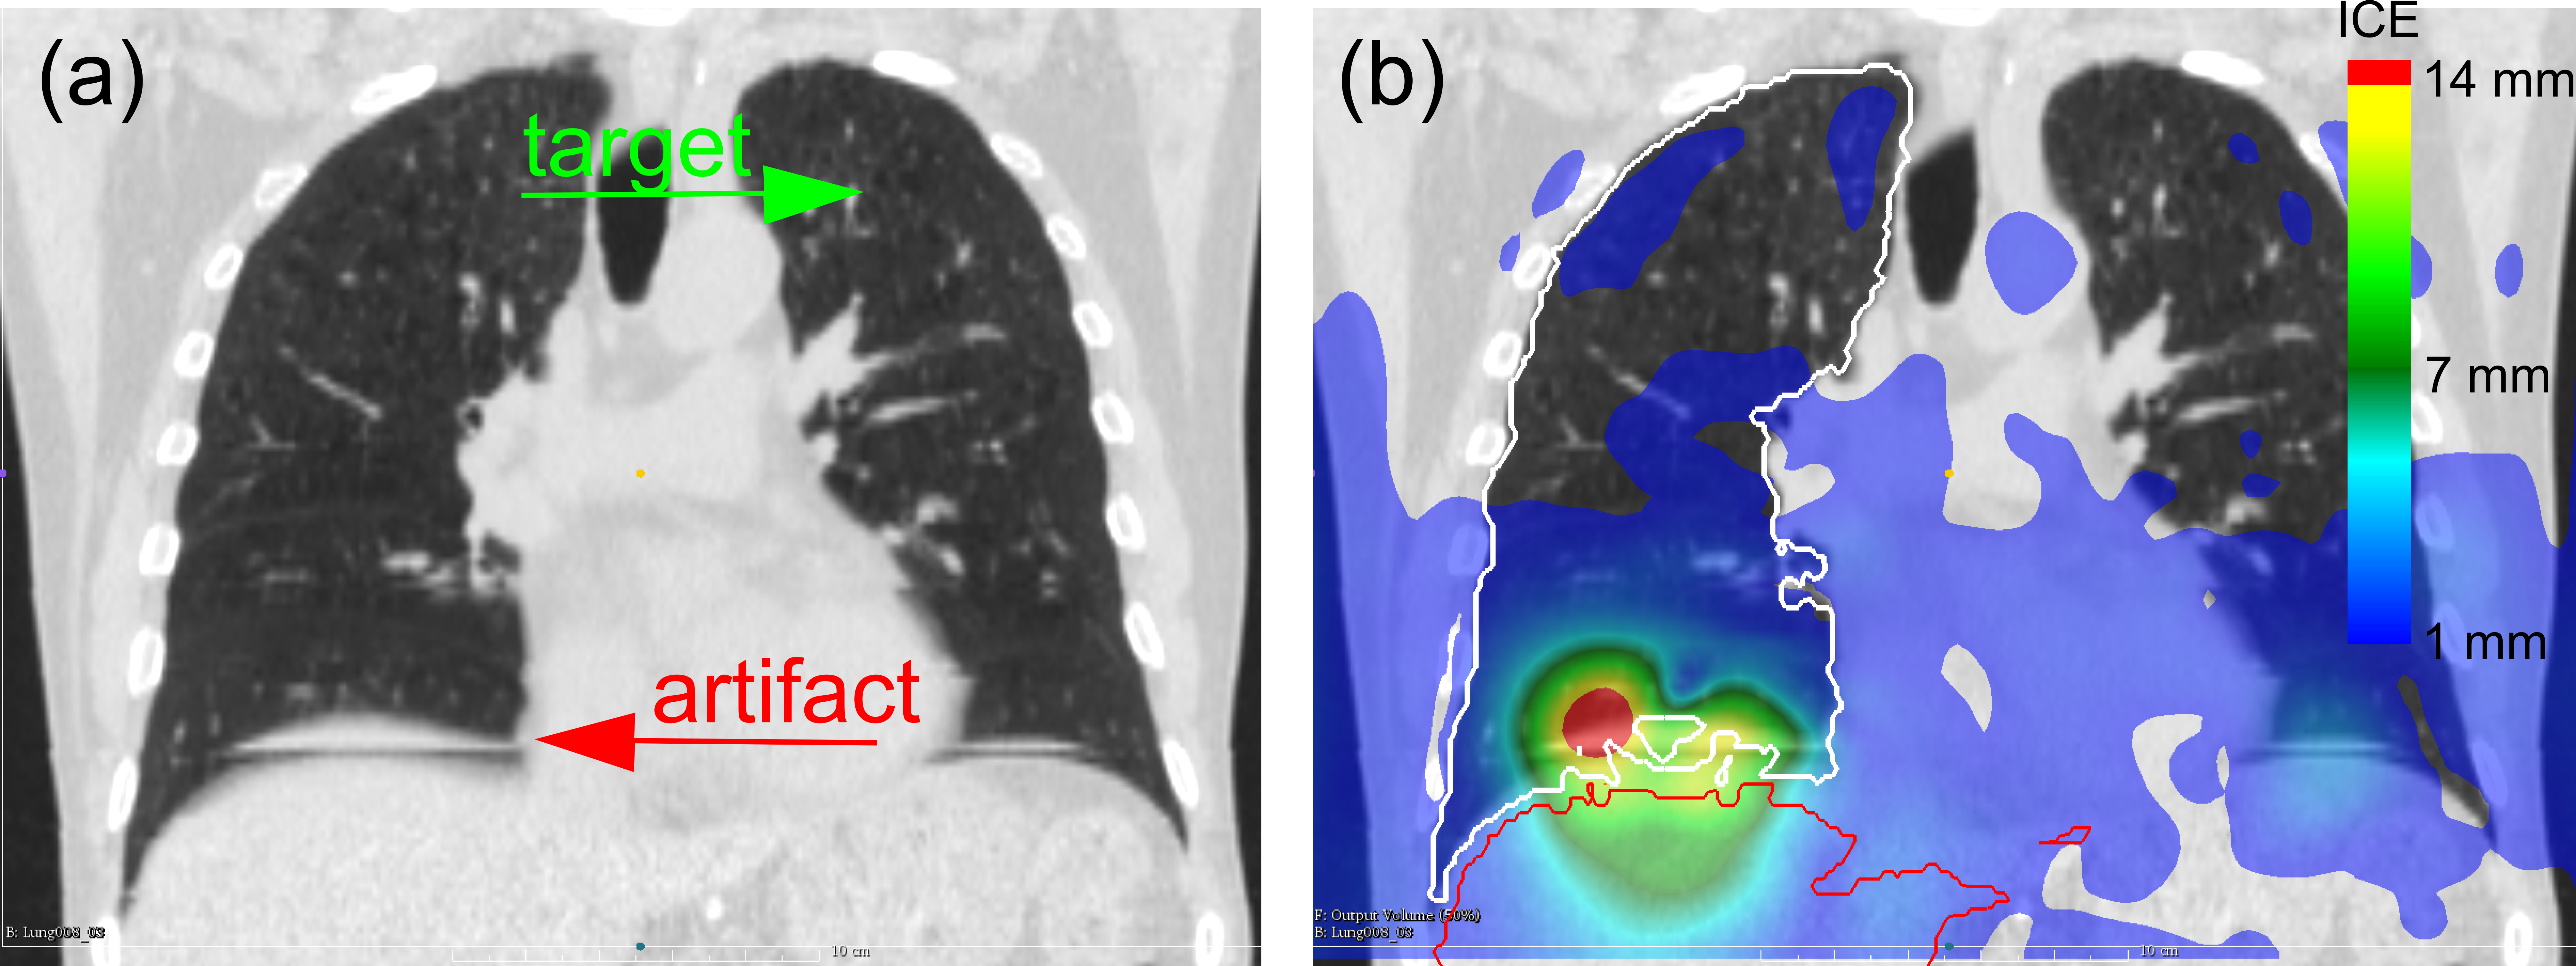
\includegraphics[width=0.9\textwidth]{./Vmm/Images/ContourPropagation/contourPropagation.png}
		\caption{Example of a contour propagation with an inconsistent DIR.(a) shows the location of 4D-CT artifact (red) and the location of the target (green). 
		The distance between them is big enough, that artifact does not affect treatment planning. 
		The large ICE is shown in (b) along with a propagated lung and liver contour. The errors in DIR result in a non-continuous diaphragm. Lungs are outlined in white and liver in red.}
		\label{contourPropagation}
	\end{center}
\end{figure}


\newpage
\subsection{Pig heart 4D-CT data}

Atrial fibrillation is the most common type of cardiac arrhythmia, causing a quivering motion of the atrial small heart chamber. 
Although atrial fibrillation directly is not a life threatening condition, it worsens the patient's quality of life and increases the risk of a stroke \cite{Benjamin1998}. 
A common method for treating the atrial fibrillation is a catheter ablation \cite{January2014}. The success rate of a catheter ablation is still limited and 
can lead to major complications or even death of a patient \cite{Cappato2005,Cappato2010}.

As an alternative treatment, carbon-ion therapy was proposed \cite{Bert2012} and later the feasibility was shown on a beating heart experimentally \cite{Lehmann2015b}. 
In 2014 a pilot experiment was performed at GSI using large animal model (pigs) and
scanned carbon-ion to verify the treatment in vivo \cite{Graeff2014a}.

To estimate and compensate motion of the heart during irradiation DIR of 4D-CT data was required. Furthermore, because of the actual irradiation of pigs a DIR quality had to be estimated and repeated, if necessary.


\subsubsection{Materials and Methods}


\subsubsection{Pig irradiation experiment}

DIR and DIRQA procedures will be given here, while a detailed description of the whole pig irradiation experiment can be found elsewhere \cite{Graeff2014a}. Cardiac gated contrast-enhanced CT scans (cardiac 4D-CT) were made on 15 pigs with a multidetector 64 row Siemens Somatom Definition Flash scanner 
(Siemens Healthcare, Forchheim, Germany) with 1 mm voxel and 1 mm slice spacing. There was no breathing motion present, since a breath-hold technique was used. Cardiac motion was based on electrocardiography (ECG)
and was divided into 10 sequential states (0-9). 
Eight pigs had a pacemaker implanted, because the irradiation was planned to damage the atrioventricular (AV) node and a pacemaker should compensate for that. Pigs are therefore divided into two groups, with pacemaker (PM), $n=8$, and without one (noPM), $n=7$.
The 4D-CT were acquired between 2\textsuperscript{nd} and 16\textsuperscript{th} July and the irradiation took place between 21\textsuperscript{st} and 24\textsuperscript{th} July.

After the CT acquisition, DIR on cardiac 4D-CT was calculated using the B-Spline Plastimatch module in Slicer (see Section~\ref{RegistrationImplement}). 
Details on parameters used for DIR can be found in Table~\ref{tab:stages2}. State 0 was chosen as a reference state. State 3 corresponds to a maximum heart contraction with likely
the biggest motion. All other states were registered to the the reference state with an inverse registration as well. 
A checklist was made to follow DIR and DIRQA for quality assurance. An example of a filled-out checklist is shown in Fig.~\ref{checkList}a.

Based on lung patient DIR and because of the time constraints in the study workflow, DIRQA was made only on DIR from state 5. 
DIRQA consisted of default and true absolute differences, true Jacobian and ICE. DIRQA results were stored in a text file (example shown in Fig.~\ref{checkList}b) and users checked if the values did not exceed expected ones: Mean absolute difference
should be smaller than 1; mean Jacobian  should be 1; mean ICE  should be smaller than 2 mm. A box-shaped ROI was created in Slicer to encompass the pig body and then used in all DIRQA checks.

After a successful DIR and DIRQA, vector fields were used for treatment planning and the resulting plans were used in the pig irradiation experiment.

Around 20 minutes were needed for each pig DIR and additional 20 minutes for pig DIRQA. Calculations were done on a cluster of Linux computers, each with 8 CPU cores and 32 GB RAM.

\begin{table}[H]
  \centering
%   \footnotesize
  \caption{Parameters used for Plastimatch registration.  A mean squared error metric was used. Details for each parameter can be found here \cite{Plastimatch}.}
  \begin{tabular}{c|c|c}
      Parameter & Stage 1 & Stage 2 \\
      \hline
      Resolution & 4,4,2 & 2,2,1 \\
      Grid size & 50 & 15 \\
      Regularization lambda & 0.005 & 0.005 \\
      Iterations & 200 & 100 \\
    \hline\hline
  \end{tabular}
  \label{tab:stages2}
\end{table}

\subsubsection{Post-experiment analysis}

After the completion of the animal study, a more detailed DIRQA was made, with all motion states included in DIRQA. In addition to the original checks explained in the previous section, vector field magnitudes were analyzed, 
the inverse absolute difference and the Jacobian were calculated. Paired t-tests were used to test statistical significance for vector field magnitudes between the true and inverse vector fields and PM and noPM groups. For linear fit quality estimation, 
a Pearson's r coefficient was used.

\newpage
\begin{figure}[H]
	\begin{center}		
		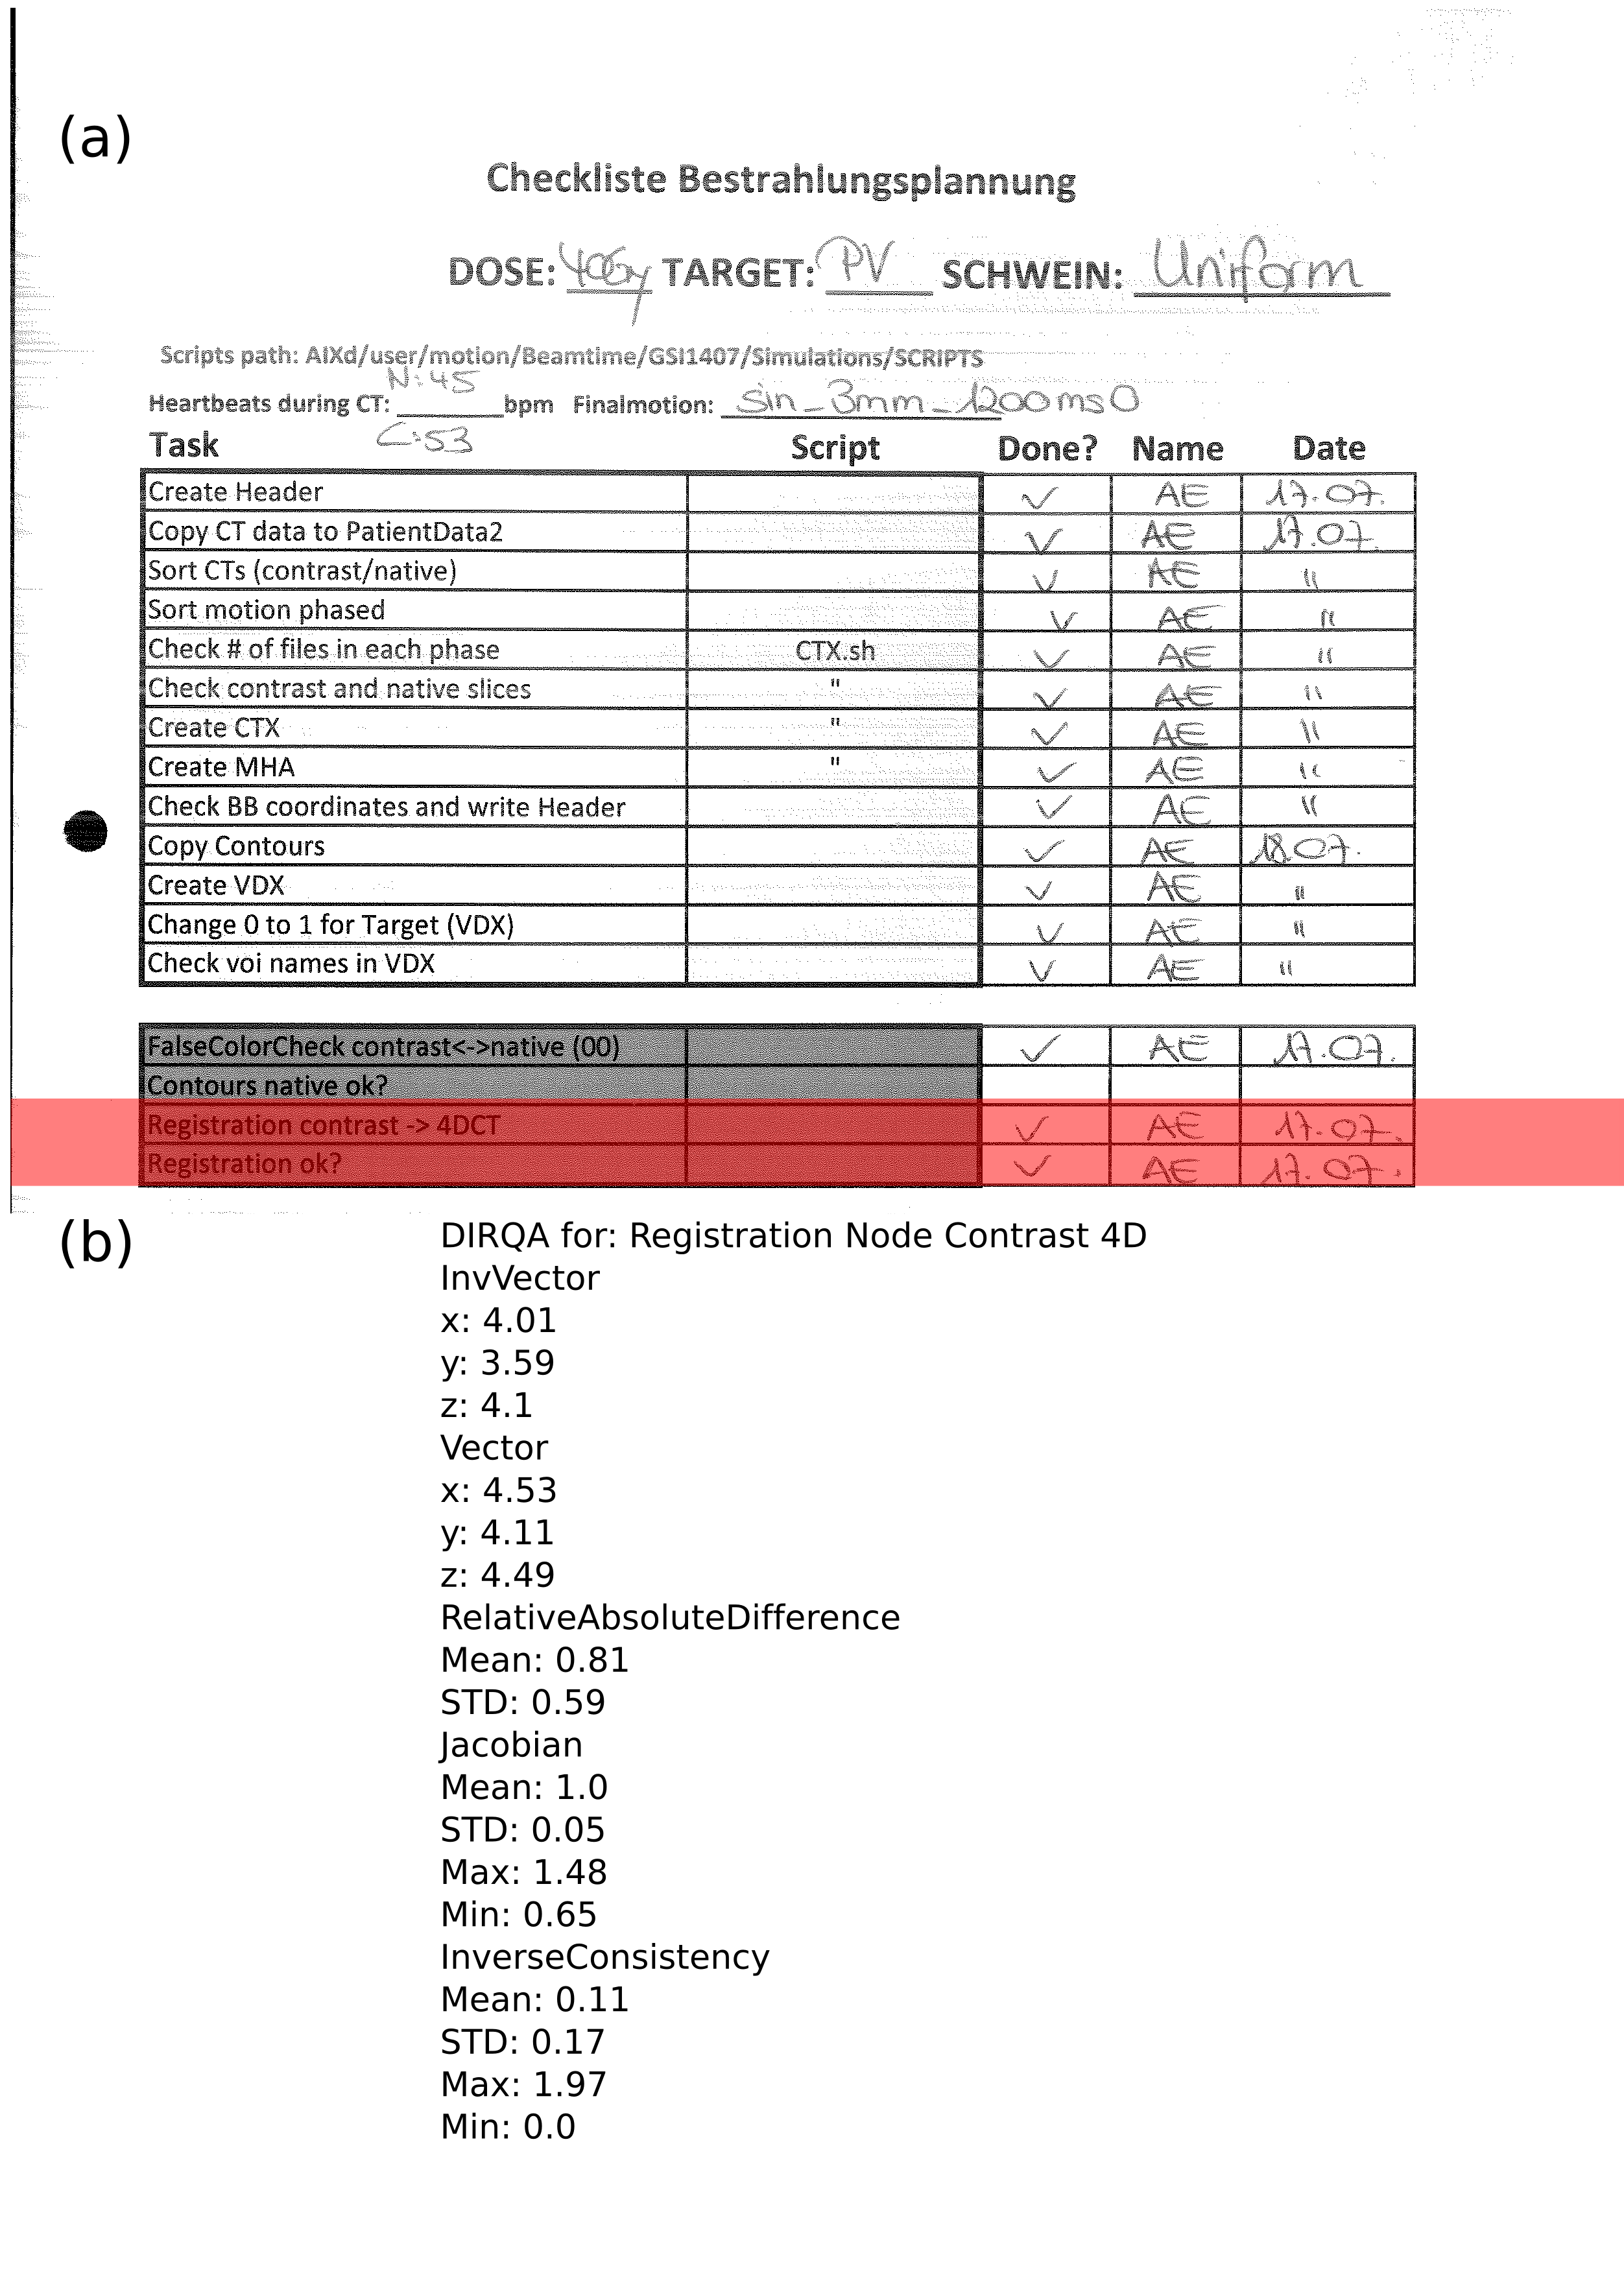
\includegraphics[width=0.8\textwidth]{./Vmm/Images/checkList.png}
		\caption{(a) A part of the checklist for quality assurance during the pig irradiation. DIR and DIRQA part is highlighted in red and consisted of two steps. First, DIR was made on a cardiac 4D-CT and afterwards DIRQA was made on
		DIR from state 50\%. The final result was presented as text shown in (b). The relative absolute difference stands for ratio between the true and default absolute difference.}
		\label{checkList}
	\end{center}
\end{figure}
\newpage
\begin{figure}[H]
	\begin{center}		
		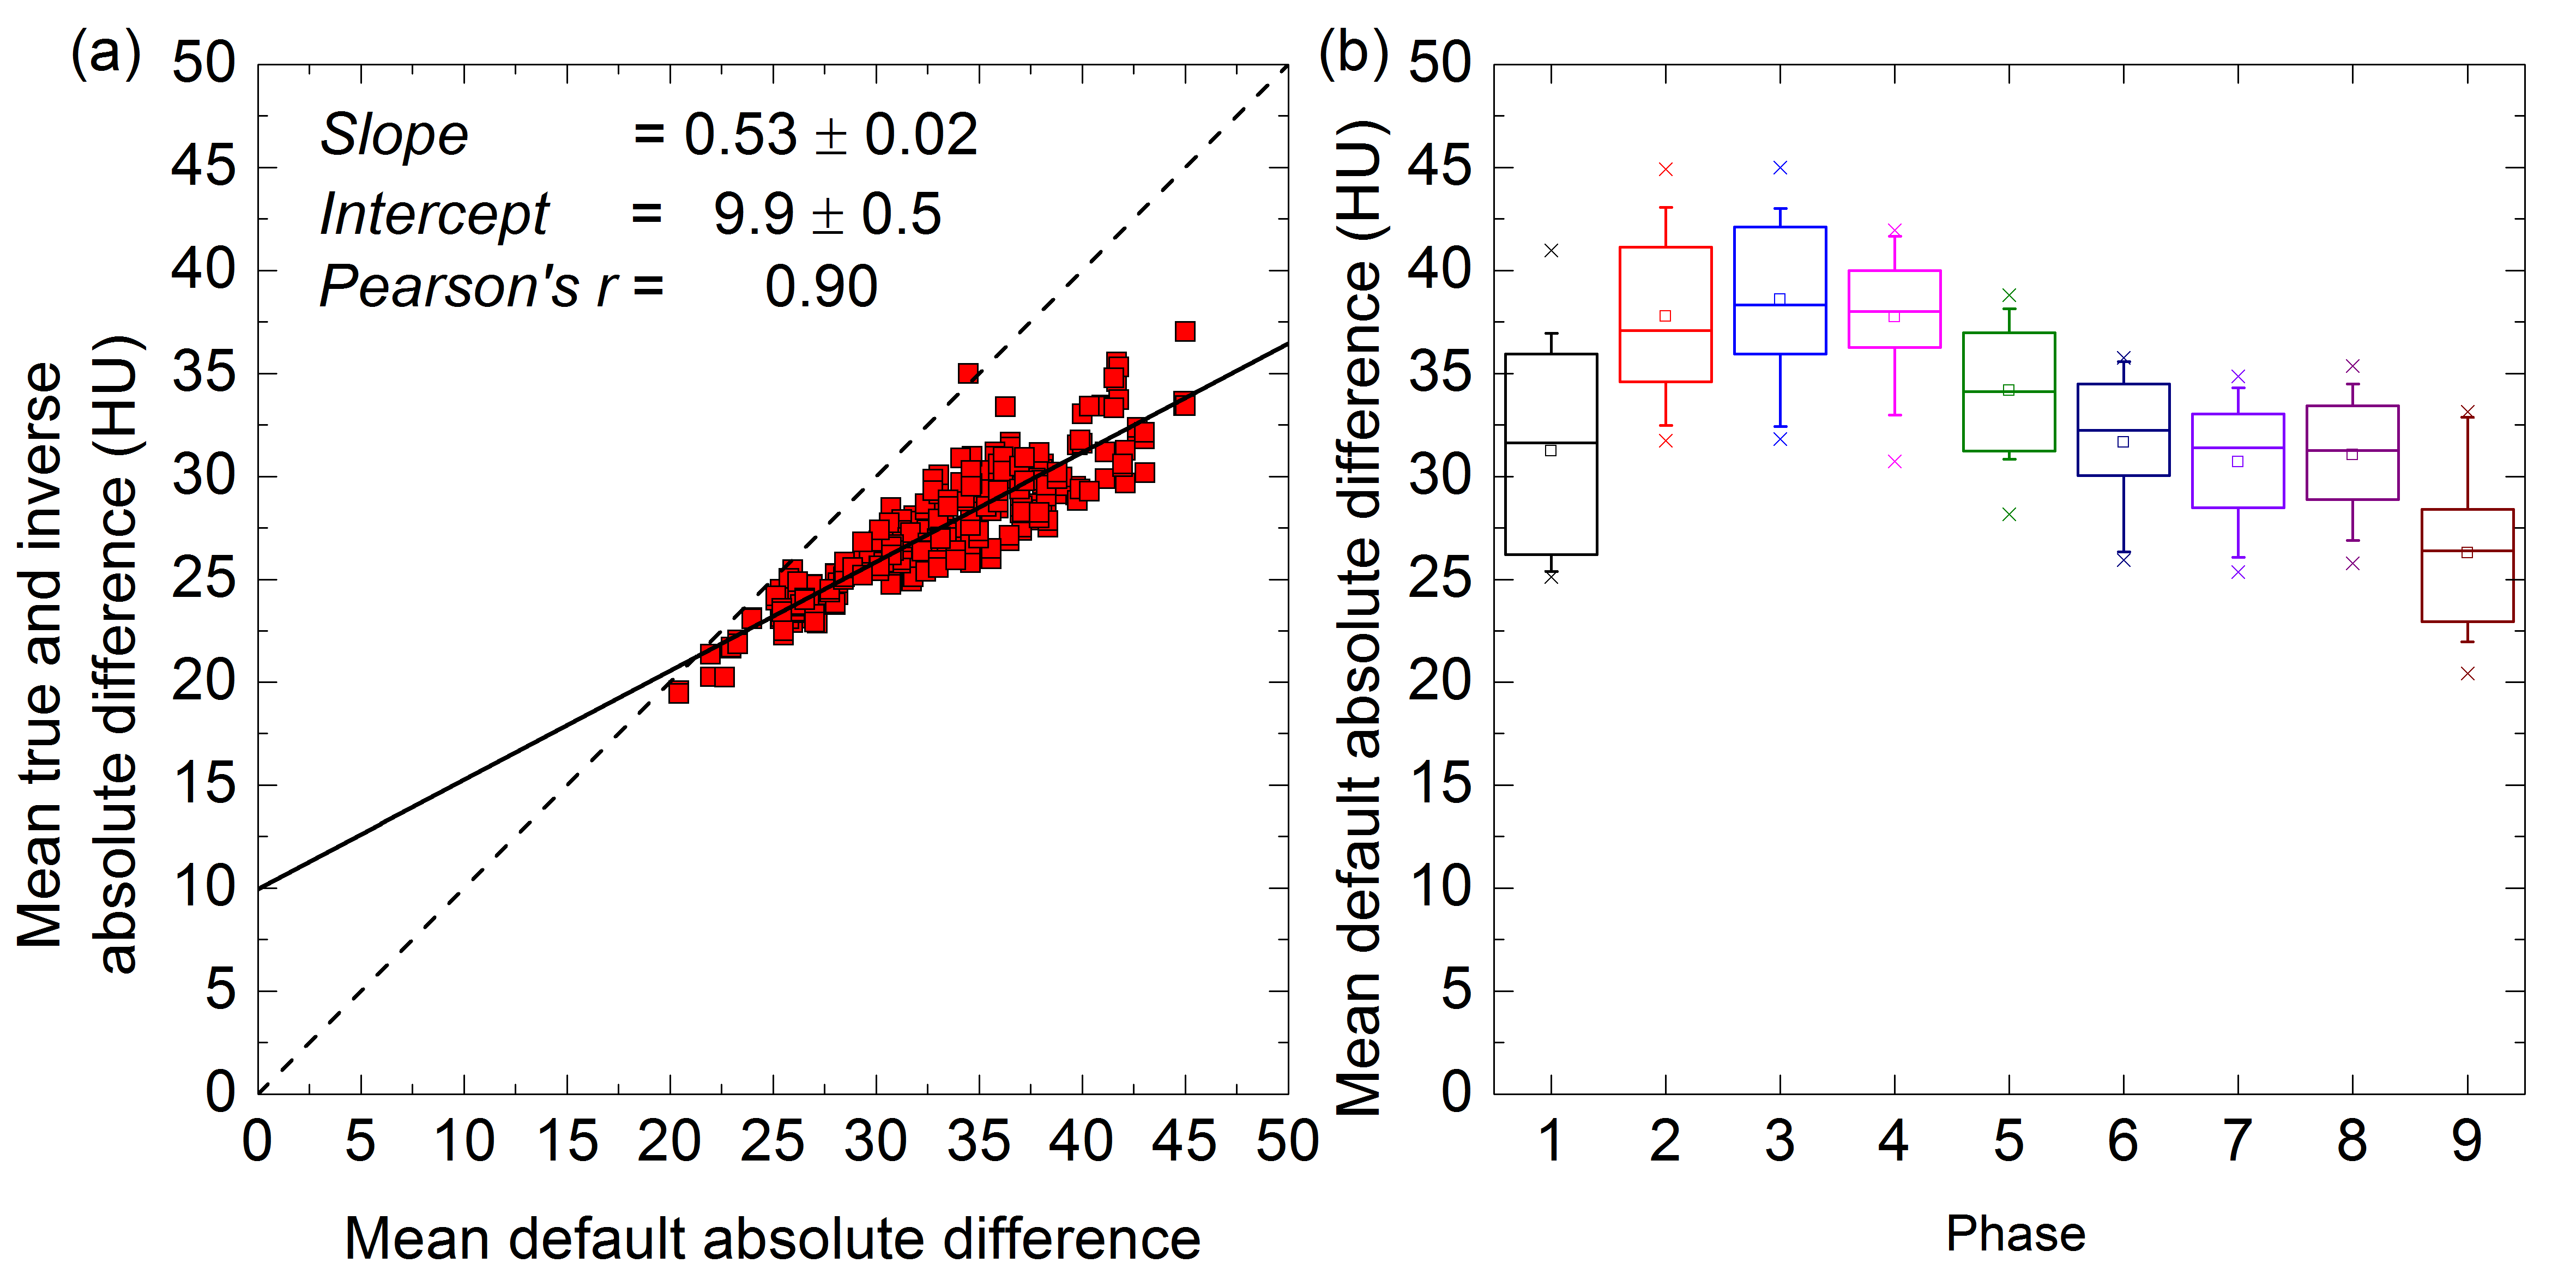
\includegraphics[width=0.9\textwidth]{./Vmm/Images/AbsDiff_pigs.png}
		\caption{(a) Mean true and inverse absolute difference plotted against mean default absolute difference. The solid line shows a linear fit, with parameters
		written in the top left corner. Dashed line shows $y(x)=x$. (b) Box plots of mean default absolute difference distribution across nine 4D-CT states. Boxes represent 25-75\%, whiskers 10-90\%
		of data. The median is shown with a solid line, the mean is represented with squares and outliers with crosses.}
		\label{absDiff_pigs}
	\end{center}
\end{figure}

\subsubsection{Results}

An example of a pig cardiac 4D-CT DIR is shown in Fig.~\ref{exampleReg_pigs}. One DIRQA during the animal study showed higher mean true absolute difference than mean default absolute difference. The registration
was therefore repeated with three stages instead of 2. The third stage had 100 iterations with resolution size ``1, 1, 1`` and grid size ''10``. All other DIRQA checks were positive.

A post-experiment statistical analysis on vector field magnitudes is shown in Table~\ref{tab:vectordata_pig}. No statistical difference was
observed between the true and the inverse vector fields. However, significant differences were observed between the vector field magnitudes of PM and noPM groups. The contributions to vector field magnitudes from three axis were equal. 


\begin{table}[H]
  \centering
%   \footnotesize
  \caption{Data for vector magnitudes. Values are presented as mean (range).}
  \begin{tabular}{c|c|c|c|c}
	    & \multicolumn{2}{|c|}{PM} & \multicolumn{2}{|c}{noPM} \\
  
            & True vector field   & Inverse vector field   & True vector field  & Inverse vector field \\
       \hline
	Mean & 0.08 (0.03 - 0.16) & 0.08 (0.03 - 0.14) & 0.07 (0.0 - 0.18)  & 0.06 (0.0 - 0.17) \\ 
	STD  & 0.4 (0.09 - 0.78)  & 0.36 (0.08 - 0.68) & 0.3 (0.05 - 0.77)  & 0.28 (0.04 - 0.71) \\ 
	Max  & 8.24 (1.6 - 17.33) & 7.98 (0.7 - 17.76) & 5.9 (0.97 - 15.91) & 5.38 (1.08 - 12.42) \\ 
    \hline\hline
  \end{tabular}
  \label{tab:vectordata_pig}
\end{table}

\begin{figure}[H]
	\begin{center}		
		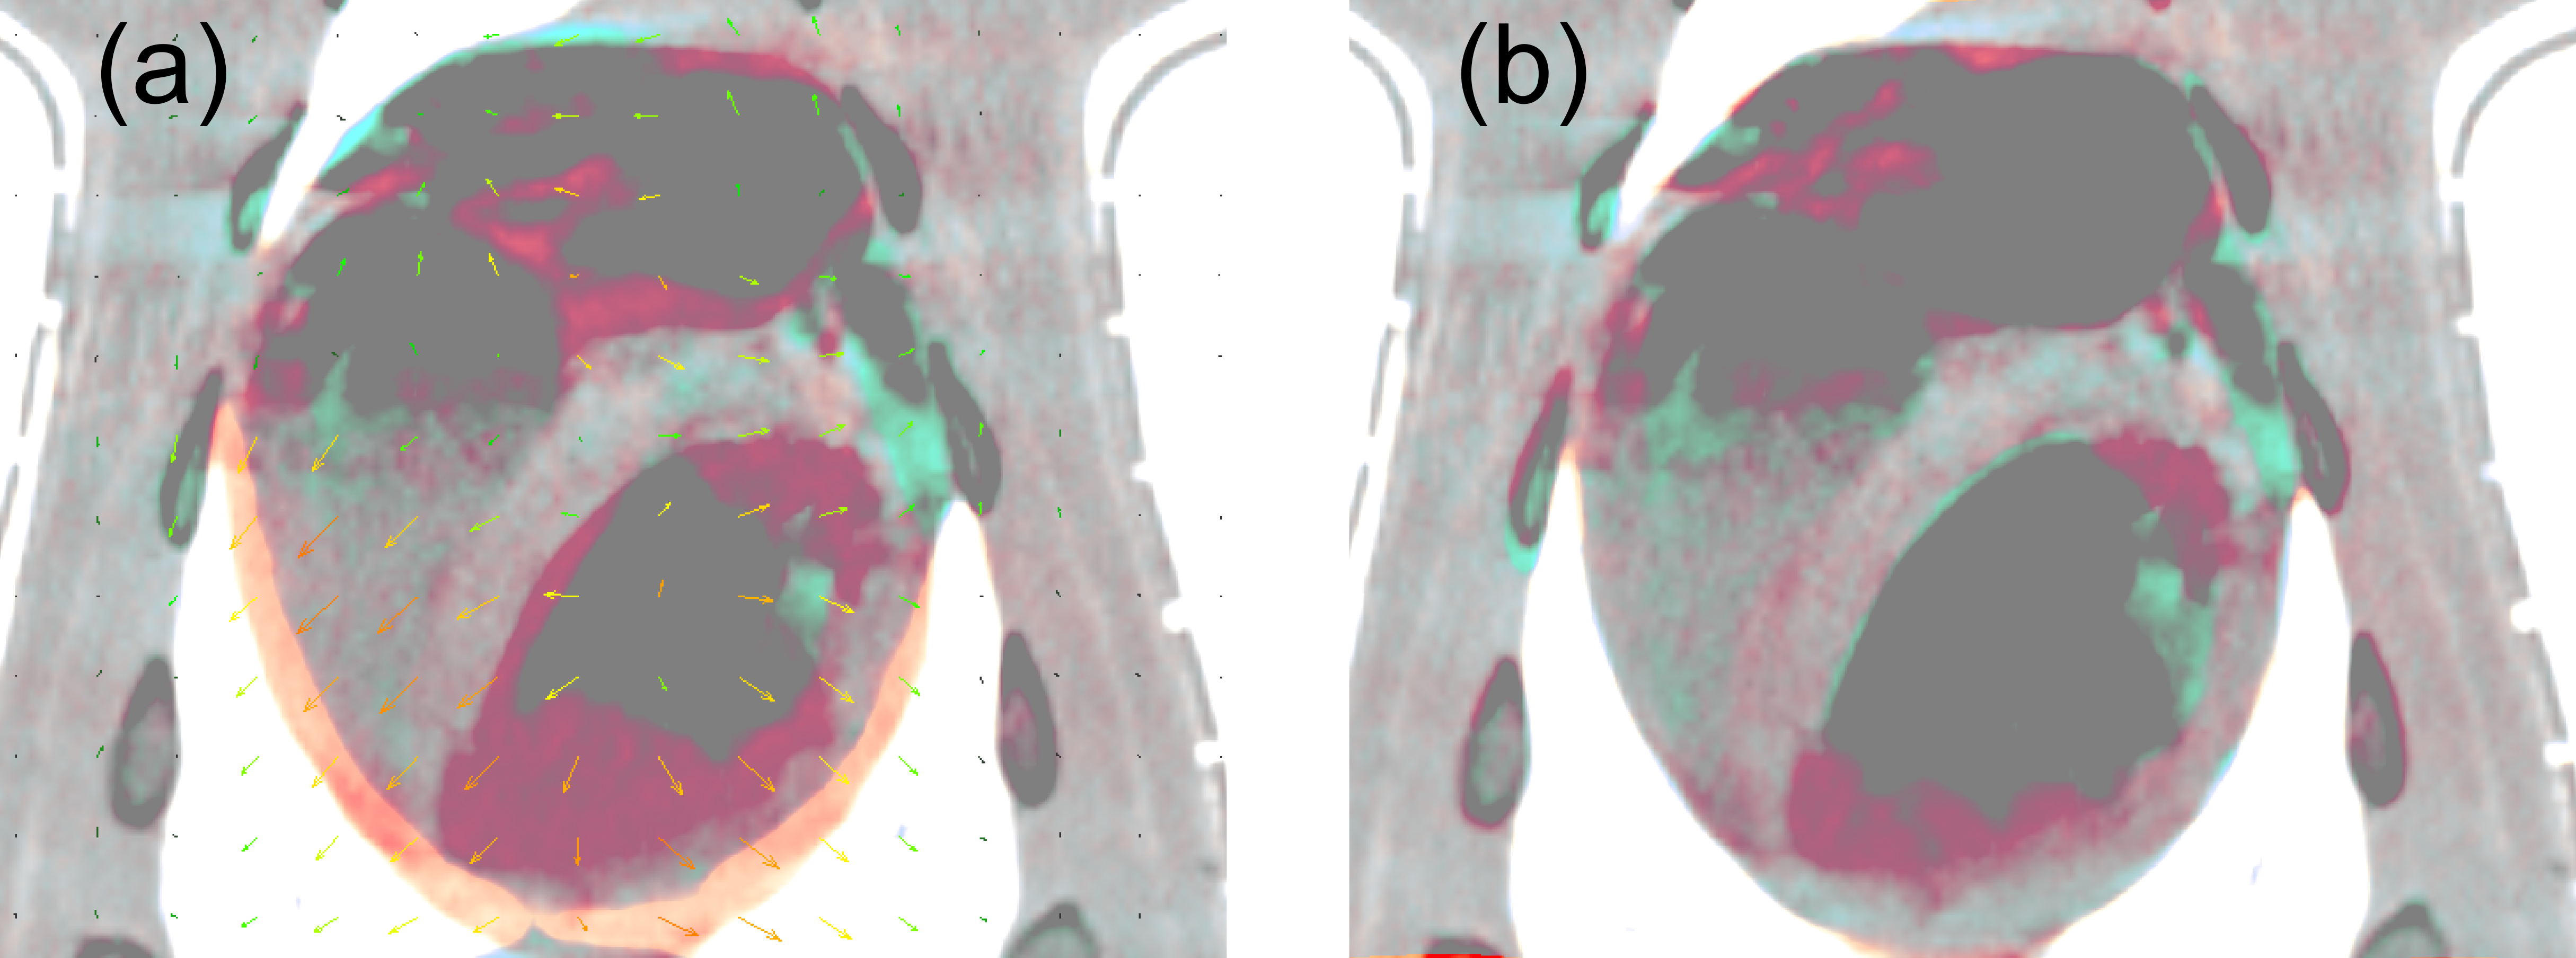
\includegraphics[width=0.9\textwidth]{./Vmm/Images/exampleReg_pigs.png}
		\caption{An inverse color overlay of two states before (a) and after (b) DIR. The vector field is displayed on image (a) as arrows.}
		\label{exampleReg_pigs}
	\end{center}
\end{figure}

The dependence of the true and inverse absolute difference on default absolute difference with a linear fit is shown in Fig.~\ref{absDiff_pigs}a. 
The default absolute difference distribution across 9 states can be seen in Fig.~\ref{absDiff_pigs}b.

The distribution of the Jacobian and ICE results are shown in Fig.~\ref{jacobian_data_pigs}. Maximum values of true and inverse Jacobian and maximum ICE were
tested against maximum vector magnitudes and fitted with a linear function. Results are plotted in Fig.~\ref{maxvf_pigs}.

All linear fits in Fig.~\ref{absDiff_pigs} and ~\ref{maxvf_pigs} were statistically significant (p < 0.05).



\newpage

\begin{figure}[H]
	\begin{center}		
		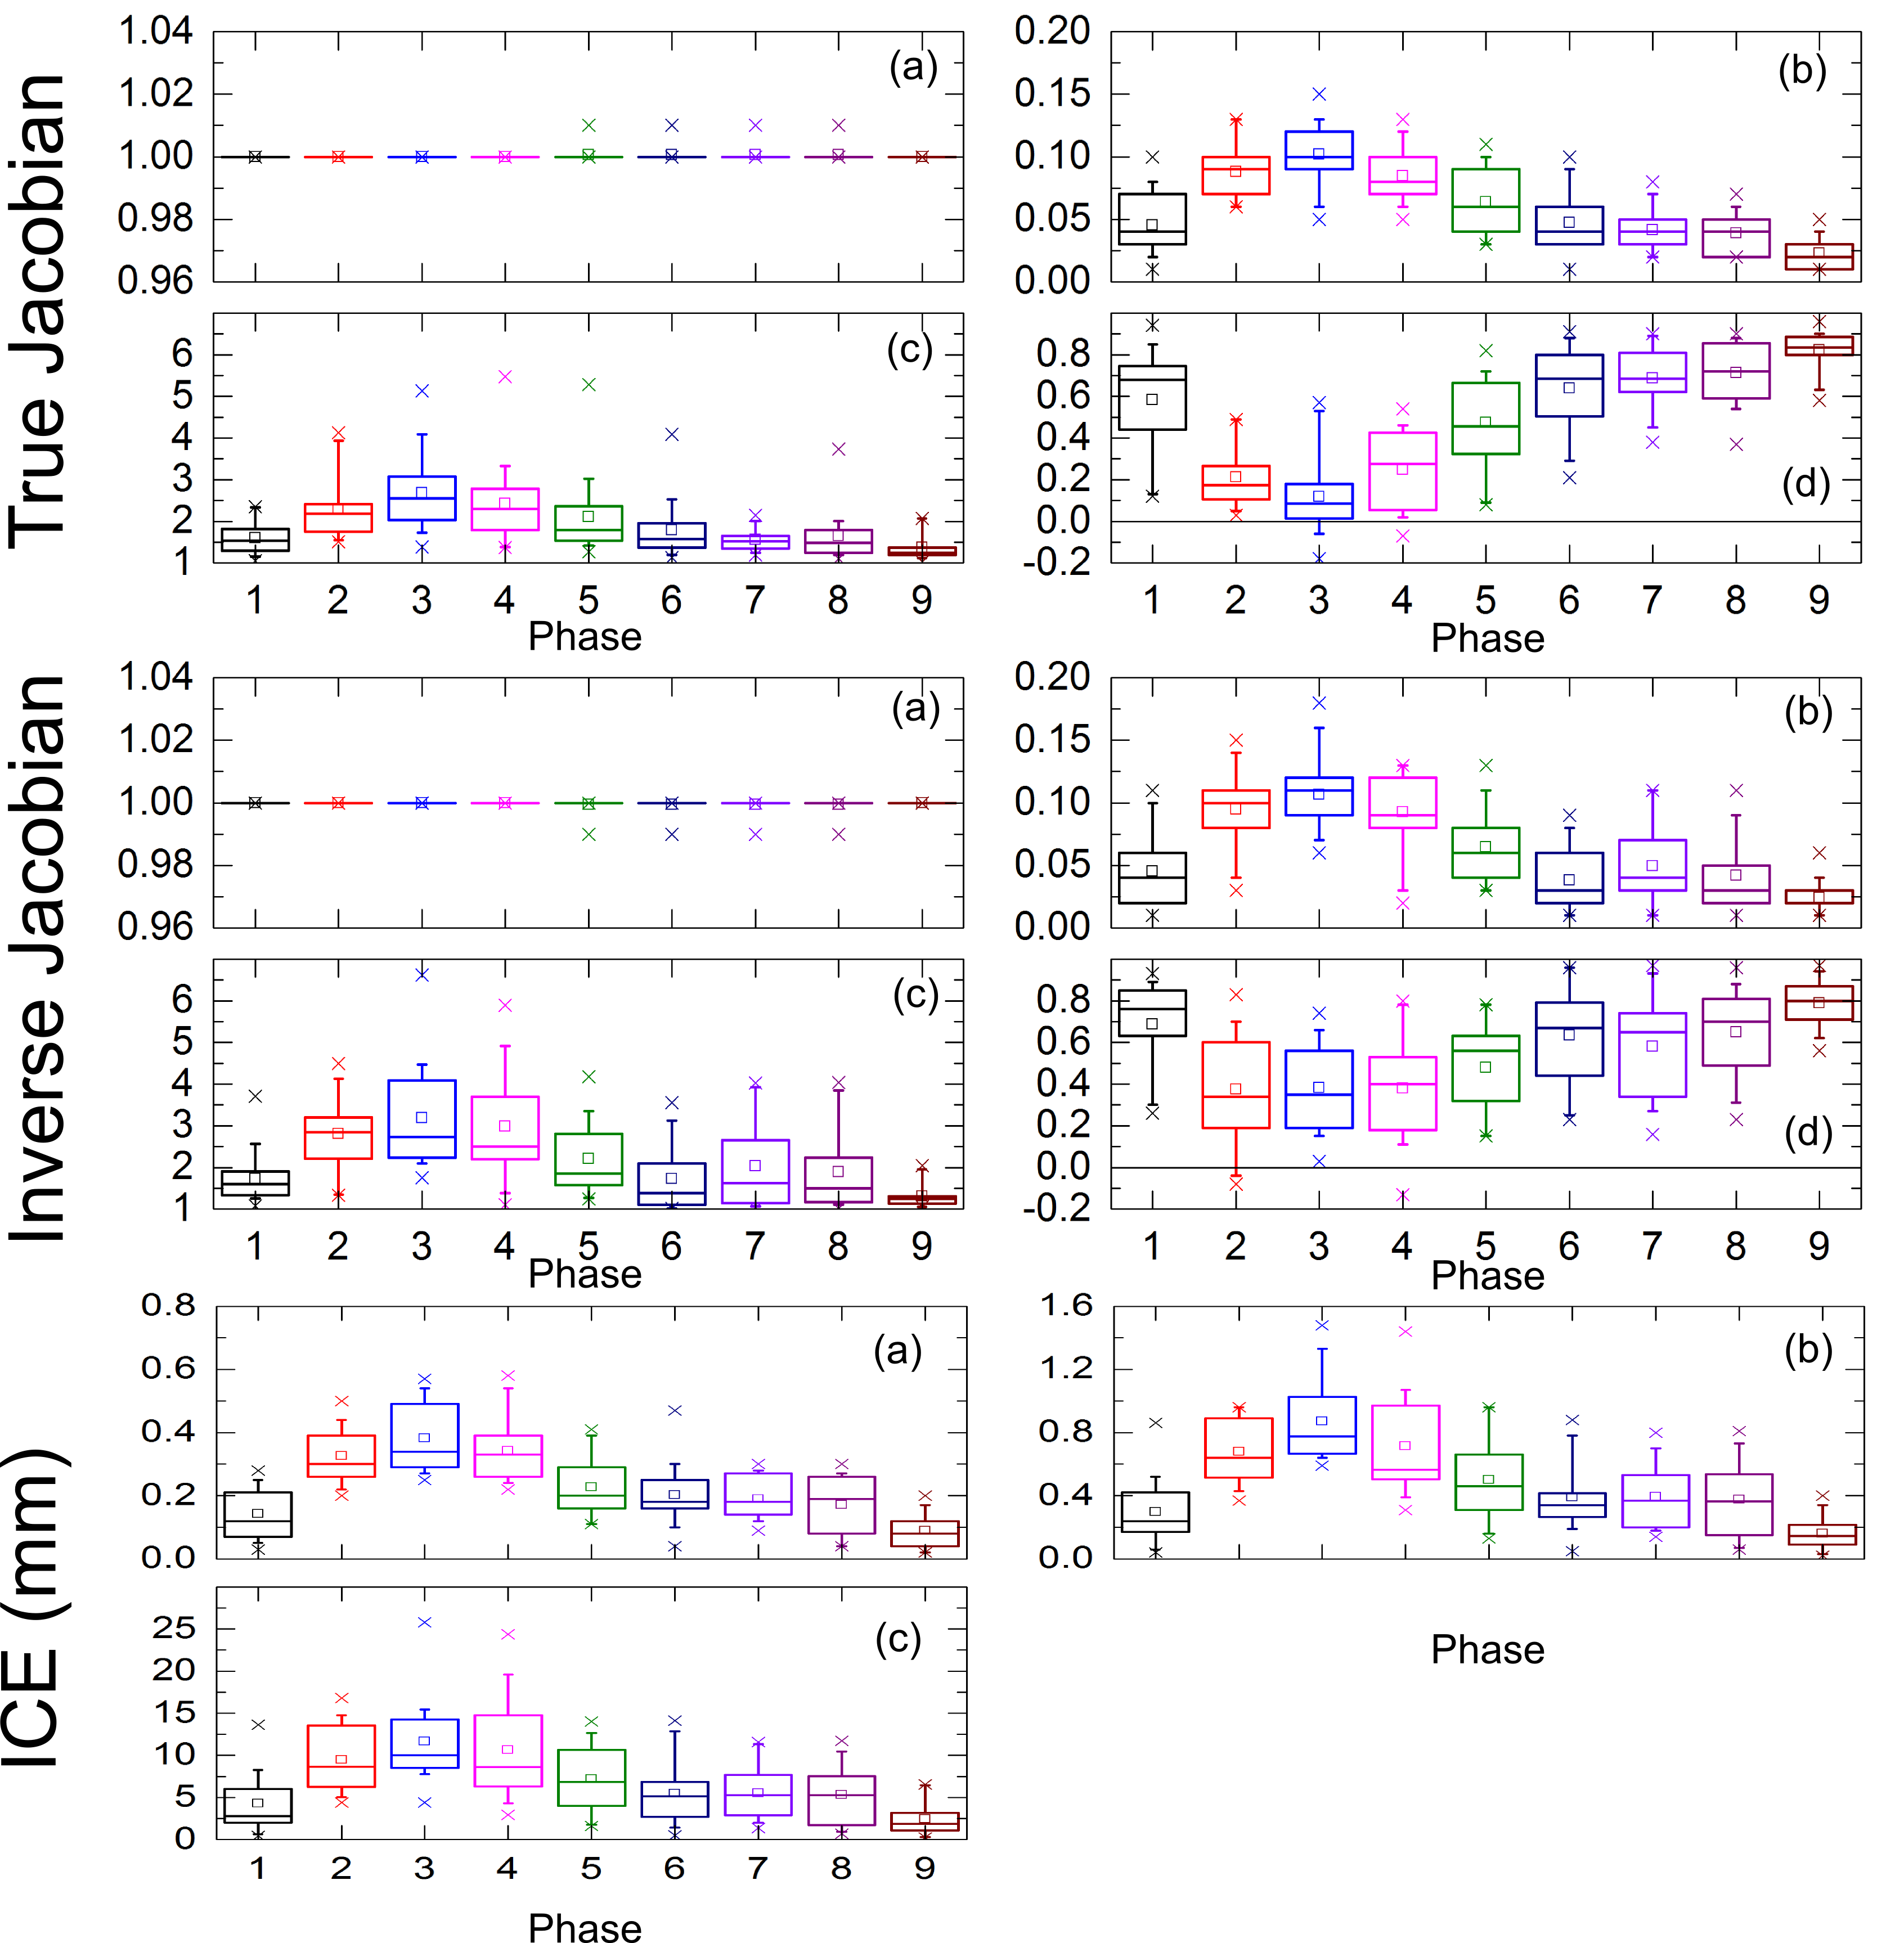
\includegraphics[width=0.75\textwidth]{./Vmm/Images/Jacobian_data_pigs.png}
		\caption{Statistical data for true (top) and inverse (middle) Jacobian and ICE (bottom) for 9 cardiac 4D-CT states (reference state 0 is excluded) for 15 pigs. Mean, STD, maximum and minimum are represented as (a), (b), (c) and (d), respectively.
		Minimum ICE is 0 throughout all states and pigs. Boxes represent 25-75\%, whiskers 10-90\%
		of data. The median is shown with a solid line, the mean is represented with squares and outliers with crosses.}
		\label{jacobian_data_pigs}
	\end{center}
\end{figure}

\newpage

% \begin{figure}[H]
% 	\begin{center}		
% 		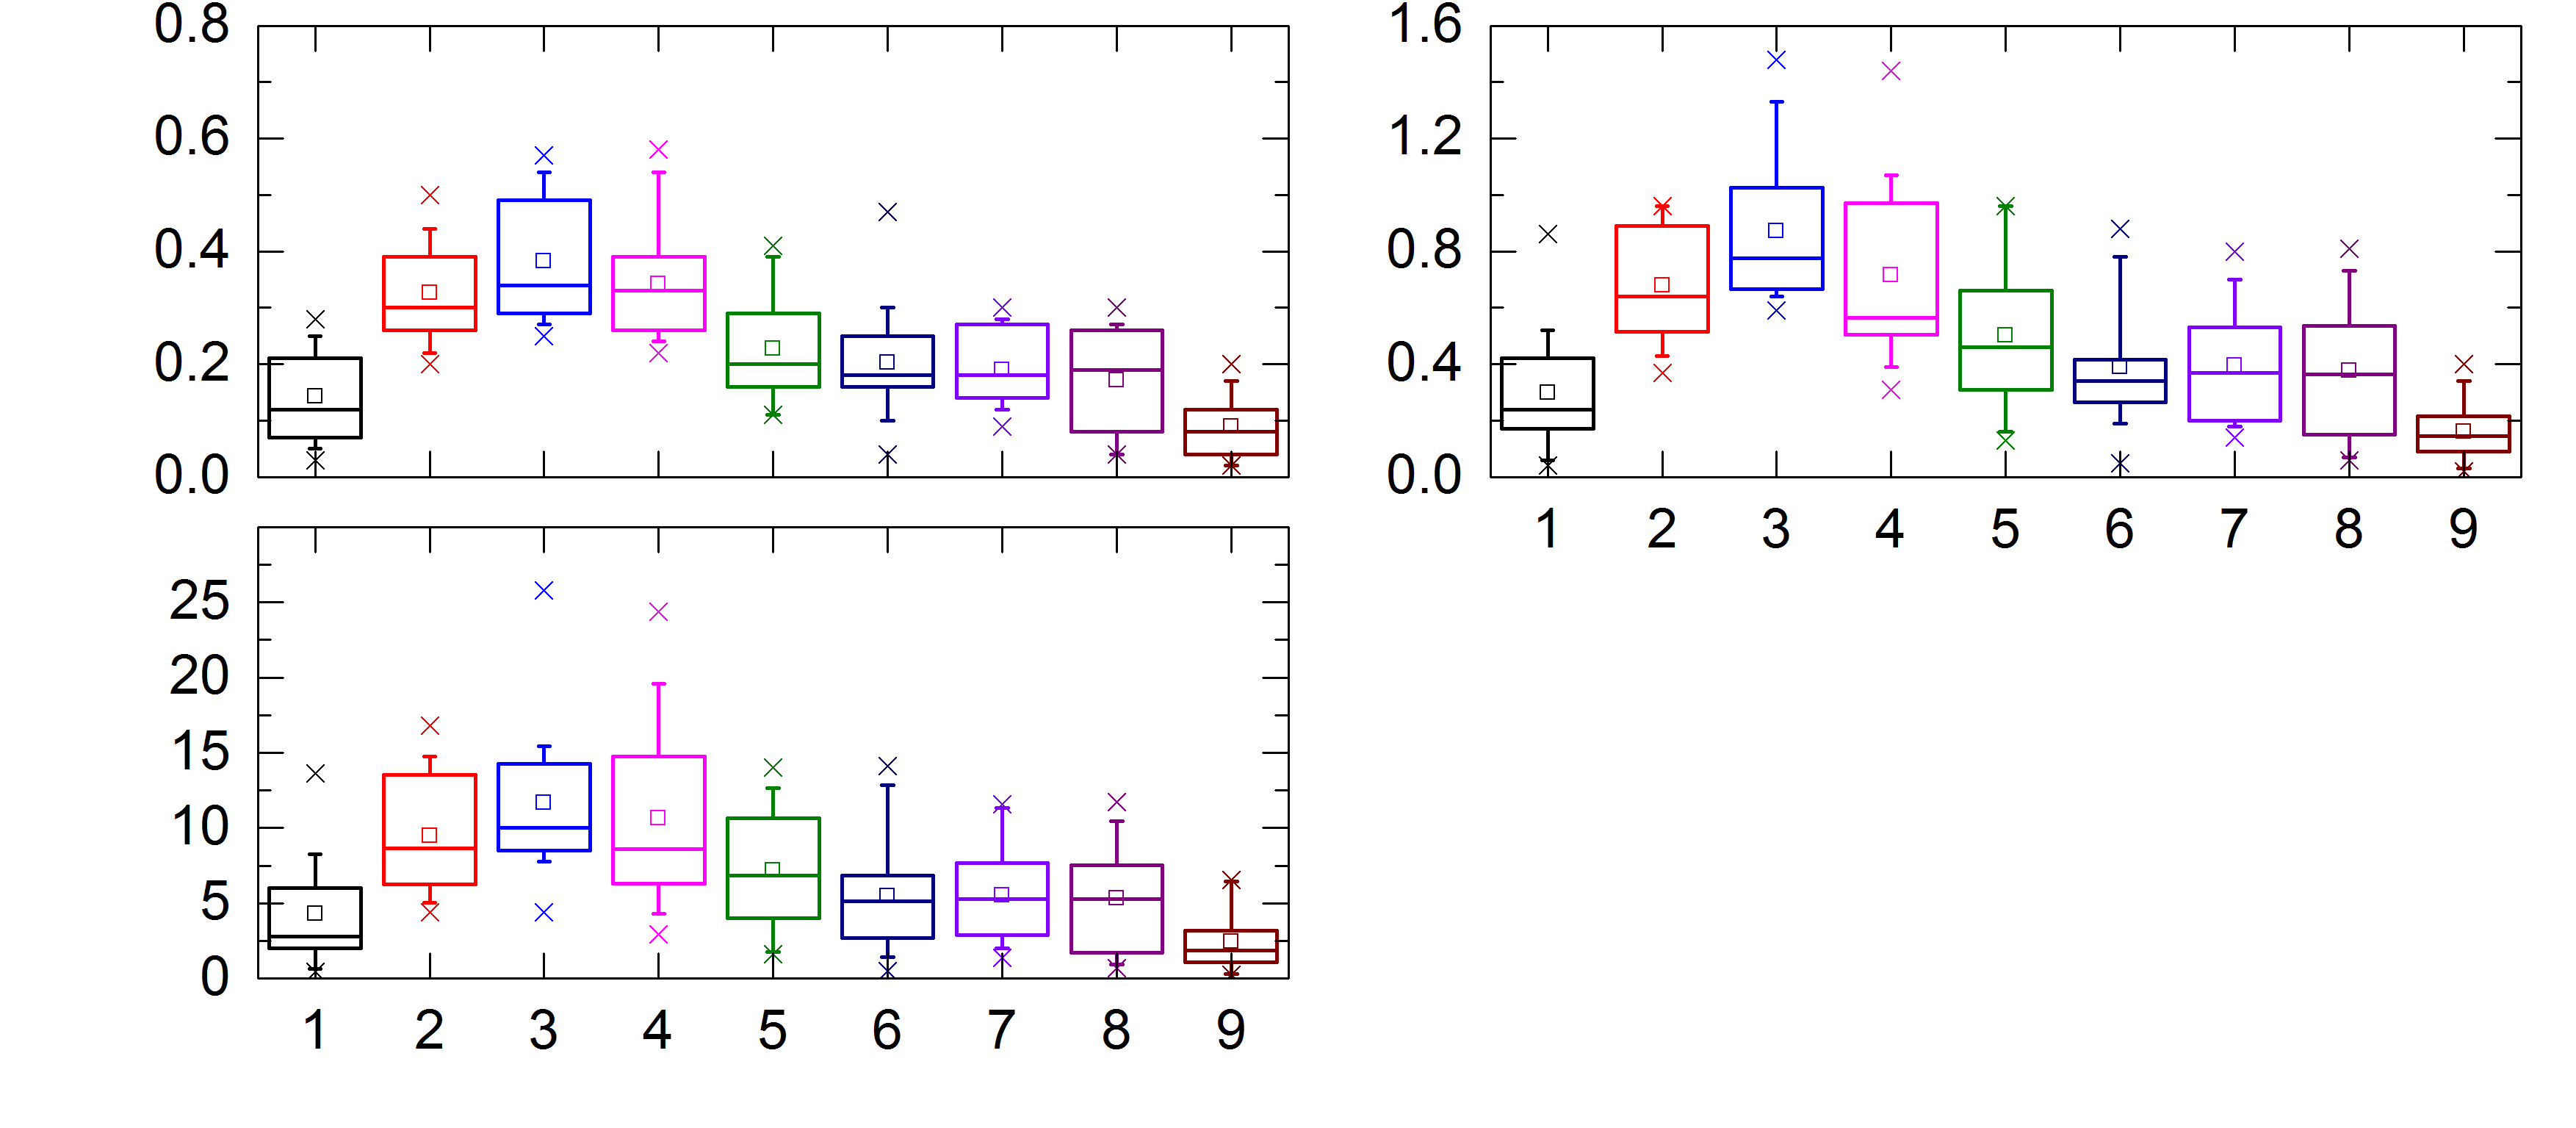
\includegraphics[width=0.9\textwidth]{./Vmm/Images/ICE_pigs.png}
% 		\caption{Statistical data for ICE for 9 4D-CT states (reference state 0 is excluded) for 15 pigs. Mean, STD, maximum are represented as (a), (b) and (c), respectively. 
% 		Boxes represent 25-75\%, whiskers 10-90\% of data, median is shown with a solid line, mean with squares and outliers with crosses.}
% 		\label{ice_pigs}
% 	\end{center}
% \end{figure}

% \begin{figure}[H]
% 	\begin{center}		
% 		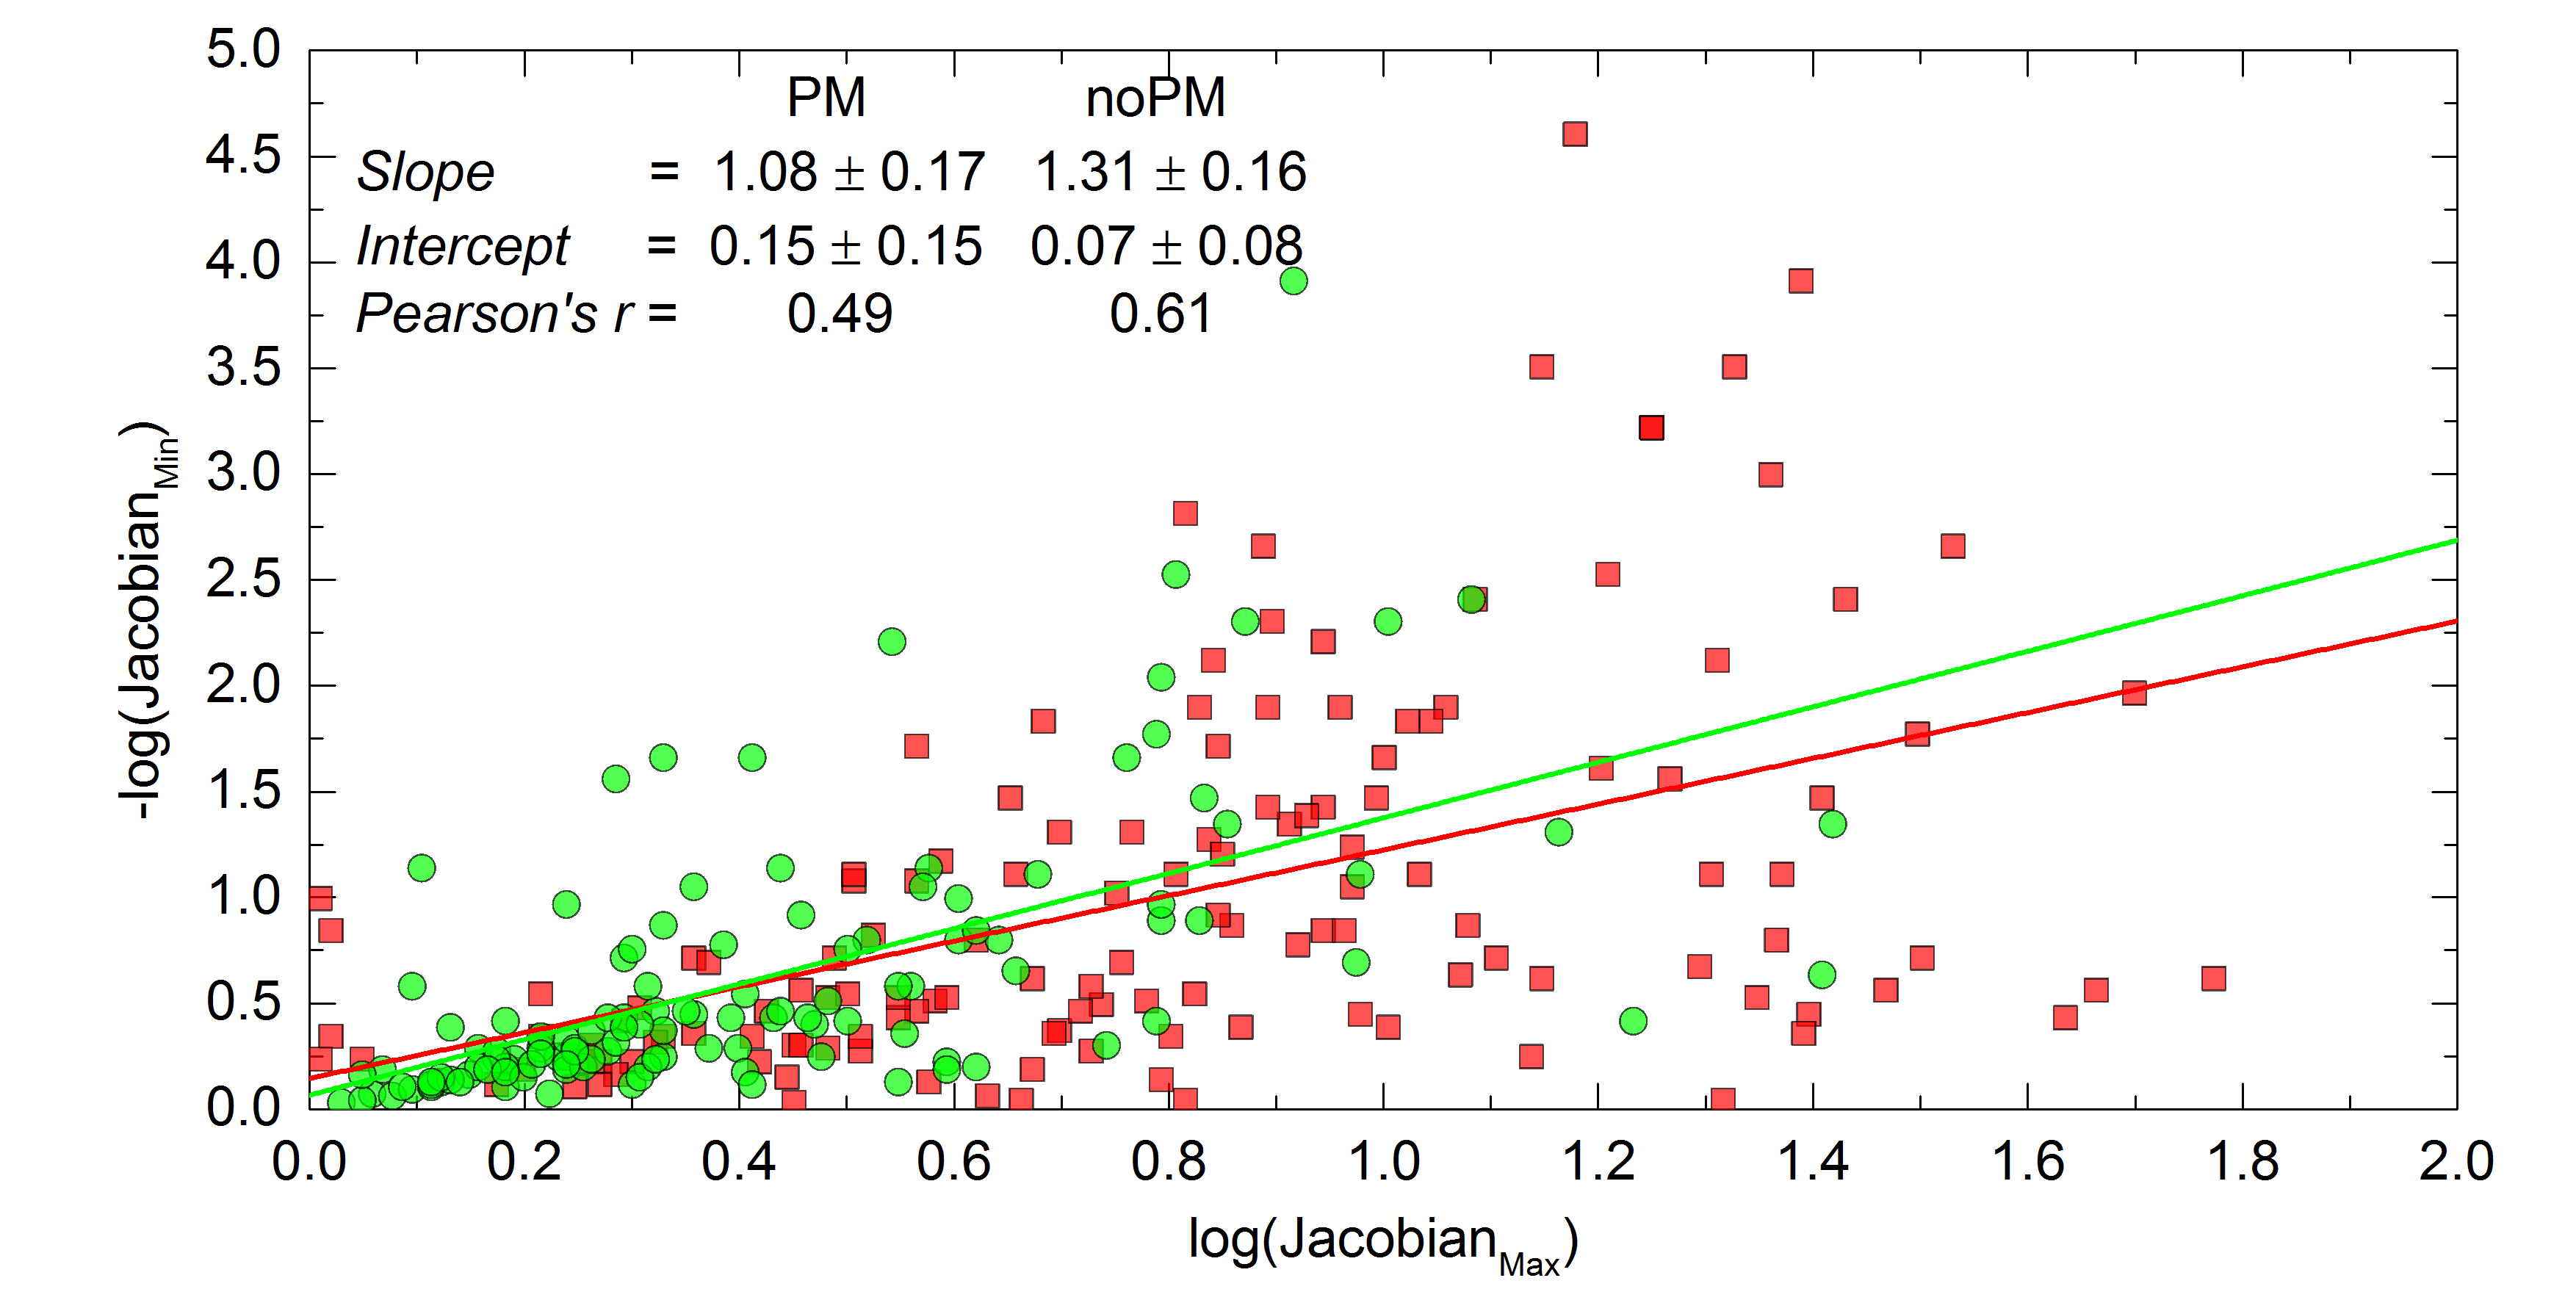
\includegraphics[width=0.9\textwidth]{./Vmm/Images/JacSum2.png}
% 		\caption{(a) Plot of negative natural logarithm of minimum Jacobian versus natural logarithm of maximum Jacobian. Linear fit is displayed with solid line and it's parameters are given in the corner. PM and noPM are shown with red squares and green circles, respectively.}
% 		\label{calcJac_pigs}
% 	\end{center}
% \end{figure}

\begin{figure}[H]
	\begin{center}		
		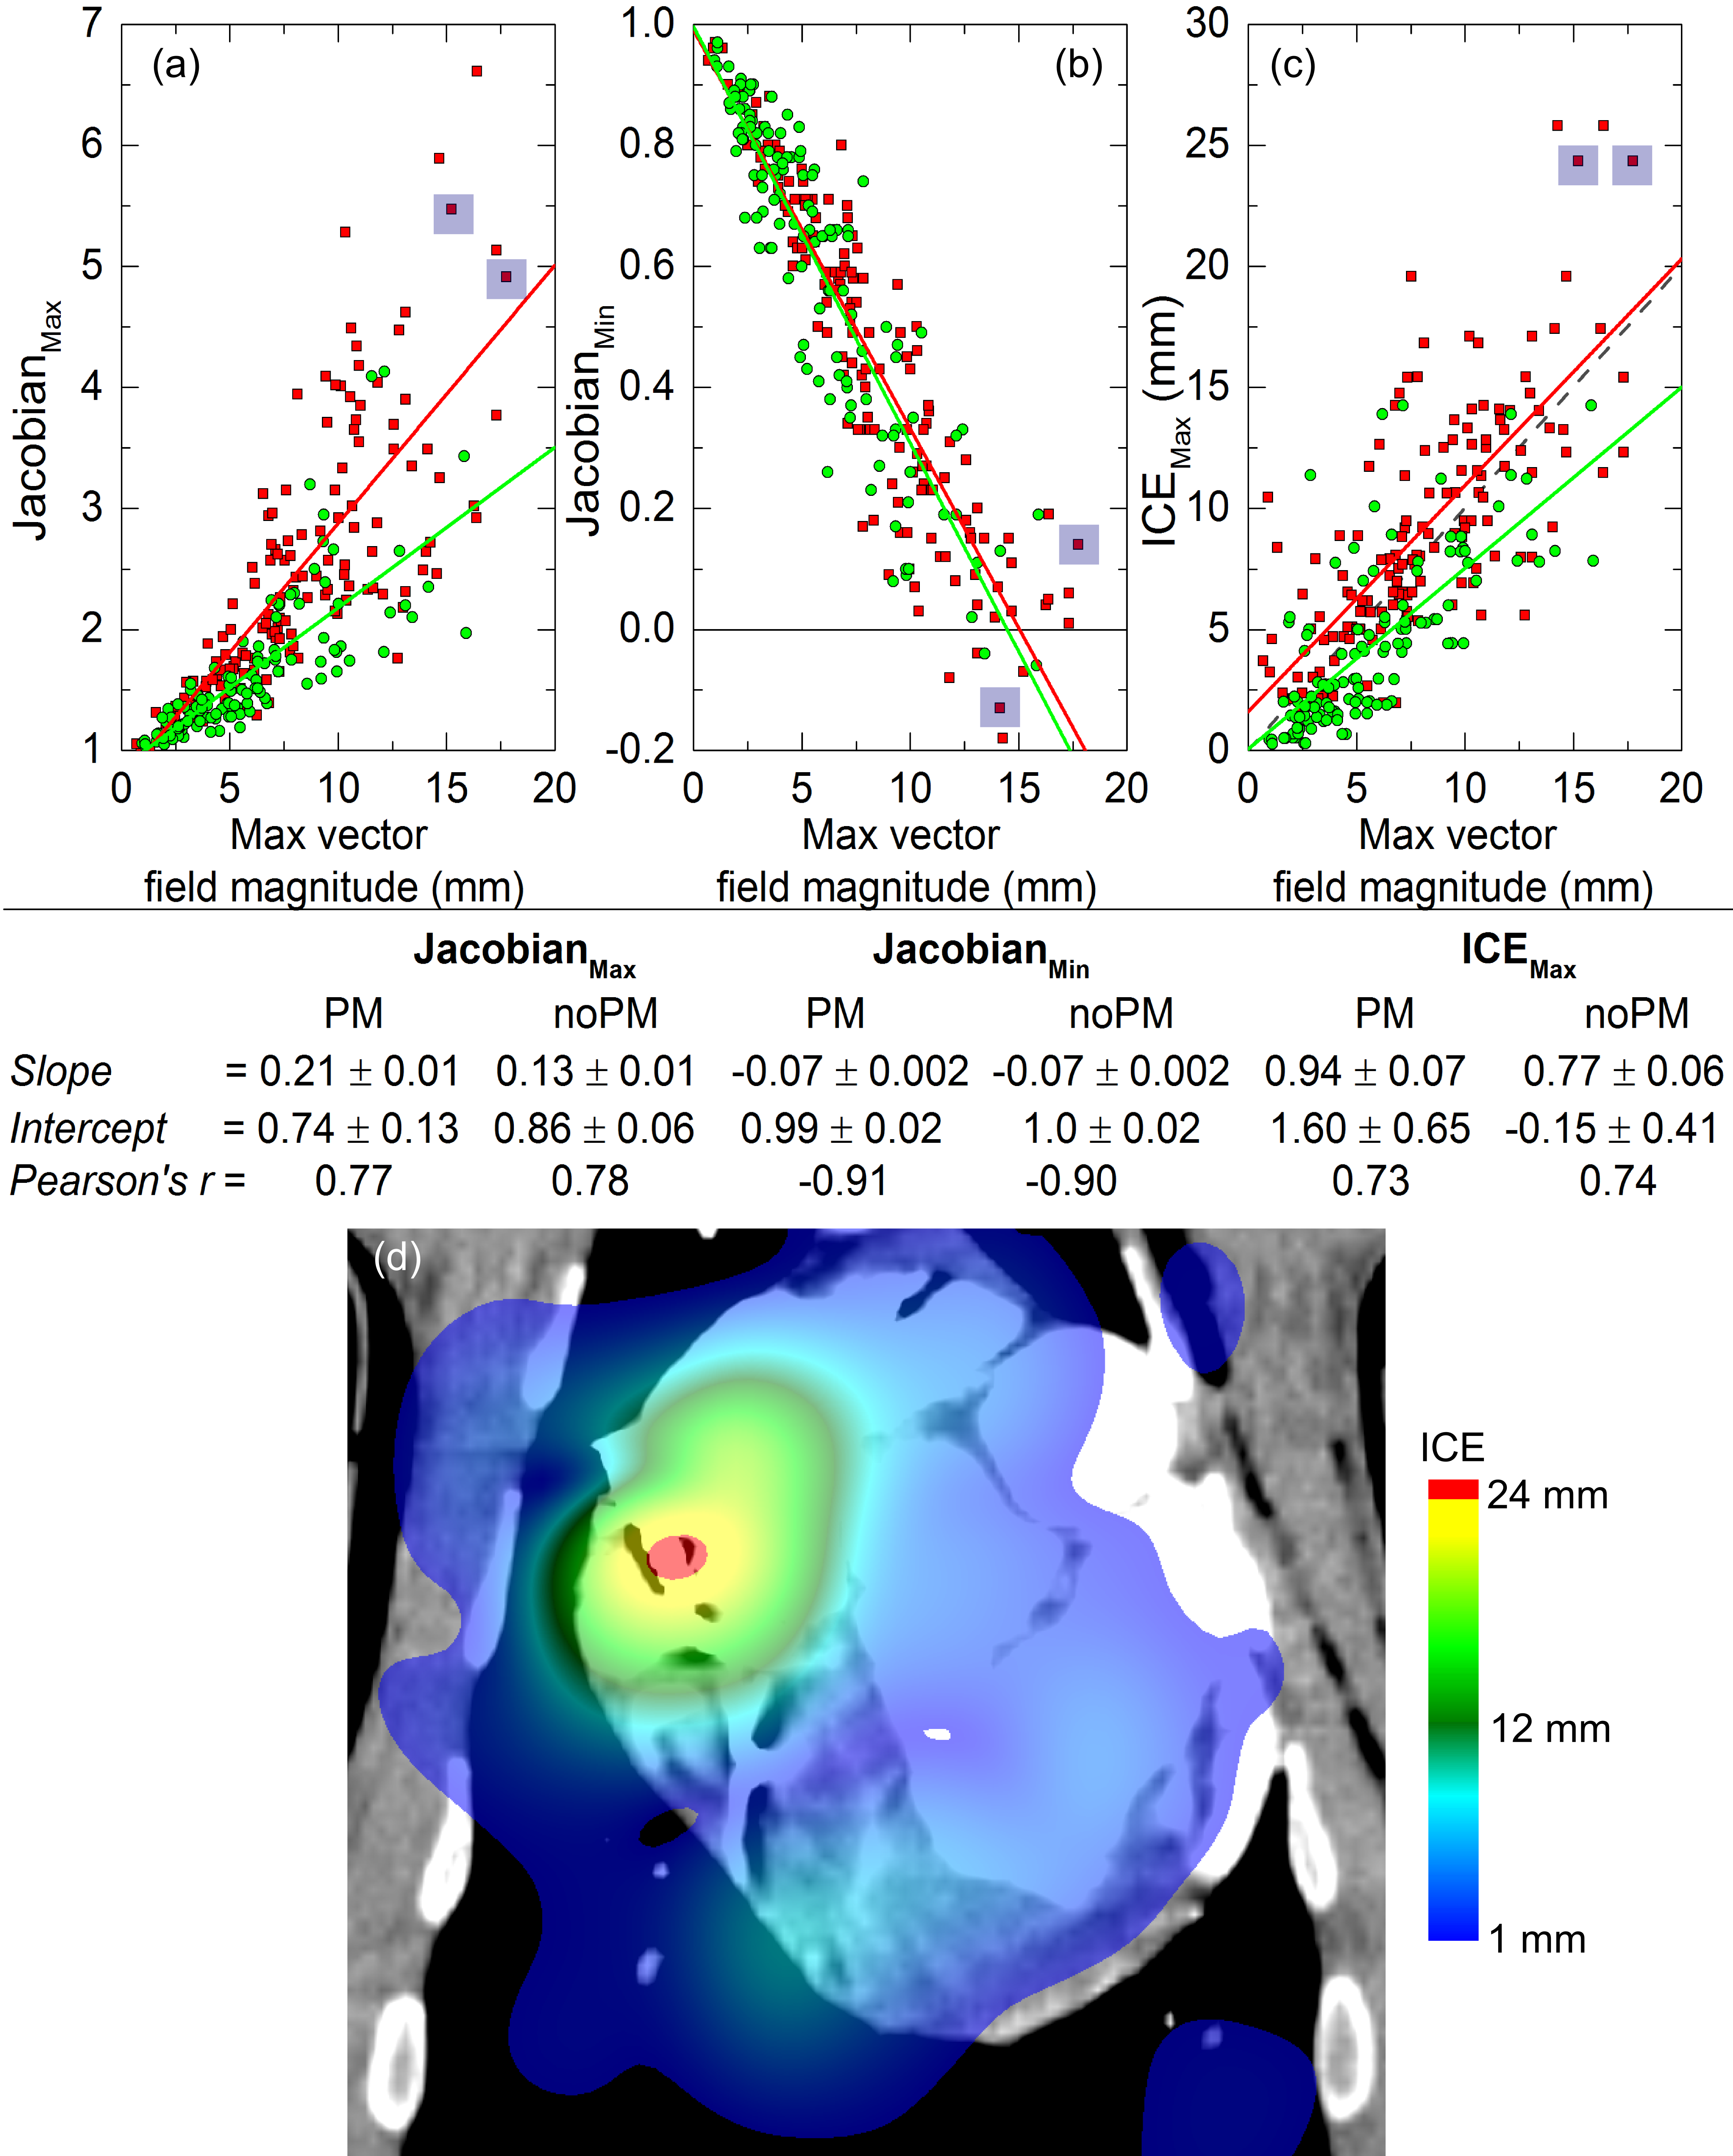
\includegraphics[width=0.9\textwidth]{./Vmm/Images/MaxVfdata_pigs.png}
		\caption{Values of maximum Jacobian (a), minimum Jacobian (b) and maximum ICE (c) plotted against maximum vector magnitudes. A linear fit is displayed with a solid line and
		its parameters are written below the plots. The dashed line in (c) shows $y(x)= x$ plot. Values from cardiac 4D-CT state on image (d) are highlighted with blue squares in (a)-(c). PM and noPM are shown with red squares and green circles, respectively.
			ICE is displayed on (d) using the color table as displayed in the legend.}
		\label{maxvf_pigs}
	\end{center}
\end{figure}

\subsubsection{Discussion}

All 15 pig 4D-CTs have been registered, which resulted in 270 DIRs. DIRQA was performed in two steps - a smaller DIRQA during animal study on one state and a complete DIRQA on all 4D-CT states afterwards.

Mean vector field magnitudes were small (approx. 0.1 mm), since pigs were in a breath-hold position and the only motion was the heartbeat. 
Despite the small mean vector magnitudes it was still enough to observe statistical difference between PM and noPM.
Consequently, the difference between the two groups is consistent throughout the DIRQA.

DIR did well in terms of lowering the absolute difference. There was a strong correlation between default versus true and inverse absolute difference. 
The slope of the linear fit on Fig.~\ref{absDiff_pigs} has the same value than the slope from lung 4D-CT (see Fig.~\ref{absDiff_lung}), showing
the effectiveness of the B-Spline algorithm. The distribution of the default absolute difference across different states is smaller than in lung 4D-CT (10 HU compared to 35 HU), due to the fact
less motion was present in a pig cardiac 4D-CT. The shape of default absolute difference
distribution persist then in the Jacobian and ICE distributions as well. 

A good result in absolute difference does not necessary mean a good DIR, as can be seen from Jacobian and ICE checks. The mean Jacobian and ICE were 1 and 0, respectively, since the
vector fields were small on average. However there were large deviations present in Jacobian and ICE. Most notably, there were a few cases of negative minimum Jacobian which would suggest 
organ folding. Since organ folding does not occur during a heart beat, negative minimum Jacobian points to inconsistencies in DIR. 

The large deviations in Jacobian and ICE can in part be explained with large maximum vector field values, as shown in Fig.~\ref{maxvf_pigs}. All linear fits have a good correlation, with no
difference between PM and noPM in the quality of the fits. The actual linear fit parameters, however, further show the inconsistencies in DIR. The clearest example of inconsistencies in
DIR is with a linear fit from maximum ICE PM, which lies above the function $y(x)=x$. This means that there were points further away from the starting point after the true and inverse transformation, 
then just after true transformation. The linear fit for noPM maximum ICE showed better results in this terms, since it lied below the $y(x)=x$ function.


During the animal study only one DIR was repeated because of DIRQA. It was shown in post-experiment analysis, that most of the DIRs should be repeated, pointing out flaws in initial DIRQA procedure.
Mainly, DIRQA should be made on all DIR and not just on one state, since DIRQA from one DIR does not guarantee the quality of the other DIRs from the same 4D-CT. 
Each DIR is performed individually and should be treated as such. Furthermore, instead of mean Jacobian and ICE, maximum and minimum should be investigated, 
because it points to the worst part of the DIR.



% \subsection{Mid-Position patient example}


\section{Summary and Discussion}
\label{Summary}

Tools to perform DIR and DIRQA have been presented in this chapter. Modules were written for an open-source software Slicer that can handle large DIR problems, such as registering whole 4D-CTs. 
In addition to DIR, the modules can also provide quantitative information on DIR quality.
The main objective of this work was to provide a systematic approach for DIR and to give parameters on DIRQA that can estimate the quality of DIR. A first analysis of DIRQA checks was done on a large DIR database - 684 DIR were checked in total.

Most of the work was based on Slicer, which is a well-established software in medical research. To date, there are more than 500 publications that have used Slicer in their research \cite{SlicerCitation}, with topic ranging from 
teaching \cite{Pujol2016}, disease staging \cite{Liu2015, Liu2016b}, motion tracking \cite{Behringer2015} to image reconstruction \cite{Meyer2015}, image registration \cite{Li2015, Fedorov2015, Li2015b}
and others. Slicer offers ample functionalities and is especially suited for research, since it can be modified to specific needs. However, it is important to stress that Slicer 
is not a medical product and as such can not be used in clinic. Additionally, Slicer can sometimes be unstable with unexpected crashes. It is constantly under development and more and more errors
are fixed with each new release. New releases also bring new functionalities, but there can be problems with backtrack compatibility. 
% Even though there are some disadvantages to using Slicer, it's advantages
% outweigh them and make Slicer a useful tool, as was shown in this chapter.

Results shown in this chapter were obtained with the B-Spline DIR algorithm. Several other algorithms exist, demons most commonly used alongside B-Spline \cite{Thirion1998}. Varadhan et al. compared B-Spline and demons DIR
for lung cases \cite{Varadhan2013} and showed that B-Spline is superior to demons, especially if there is a difference in contrast between the images. They used a mutual information
metric, to account for differences in contrast. Images used in this chapter were either all without (lung 4D-CTs) or all with (animal study 4D-CTs) contrast agent, therefore no difference in contrast
between images was present and mutual metric could not be used.
% . Mutual information metric was tested as well for DIR. For lung 4D-CT it could not complete DIR, because the states are too similar, however for the results were worse than mean square error metric. For lung 4D-CTs 

A designated module was written for DIRQA. The main advantage of the DIRQA module is that all different techniques are gathered in a single place and can be used on a specific case. 
The ease of use is also essential, for DIRQA to find its way into clinical work flow.
A test of using DIRQA in potential clinical work flow was done at GSI during the animal study, where different users operated with both DIR and DIRQA modules. The experiment was carried out under time pressure, since there was
a scheduled beam time. 4D-CTs were acquired approximately two weeks before the scheduled irradiation. During this two weeks contour delineation, DIR, DIRQA, treatment planing 
and treatment planning QA had to be done \cite{Graeff2014a}.
There were already propositions for frameworks for DIRQA in clinical work flow \cite{Varadhan2013}, however none were tested in an actual clinical environment. An animal study can not be directly compared to an actual clinic,
however the number of pigs studied was high (15) and the study was under time constraint, which simulate some of the pressures present in clinical environment.

The techniques used in DIRQA were divided into visual qualitative (inverse color, checkerboard) and quantitative (absolute difference, Jacobian and ICE). While the quantitative can be used to pinpoint errors in DIR, the visual qualitative
can be used to actually locate the error as shown in Fig.~\ref{maxvf}d. The location and size of DIR error also determines if a repetition of DIR is necessary.
All three quantitative checks have been used in literature as a possible DIRQA \cite{Varadhan2013, Leow2007, Christensen2001, Bender2009}.
They all share the same flaw, however, that they are a necessary but not sufficient condition for a successful DIR. 
One common DIRQA check in literature that our module is currently missing, is comparison of anatomical correspondence - 
comparison between reference, moving and warped contours. Ideally the warped and the reference contour should be the same. Two metrics are usually used in contour comparison -
dice similarity coefficient \cite{Varadhan2013} and Hausdorff distance \cite{Huttenlocher1993}. Slicer already has functionalities for both contour comparison checks, so they could be used. 
The biggest disadvantage of the anatomical correspondence check is that the contour delineation is required in both, the reference and moving phase, which is scarcely done by physicians, 
since it takes too much time. Additionally, the anatomical correspondence check does not judge the vector field quality inside contour.
The lack of contours in both reference and moving phase was the reason the anatomical correspondence check was not used.

Studies on DIRQA so far have focused on a small number of DIR cases, whether it is phantom \cite{Mutic2001,Moore2004} or patient studies \cite{Wu2008, Varadhan2013}. With a small number of DIRs,
it is possible to thoroughly examine each DIR and hence understand DIRQA. In this work a different approach was
used. Rather than examining each DIR individually, a large dataset was analyzed and common traits for DIR were found. Due to differences in anatomical sites, 
DIRQA parameters have to be found for each anatomical site individually, since they can
deviate significantly, as seen by two different cases presented here. However, three checks are independent on anatomical site: mean true and absolute difference should be lower than 
default absolute difference, Jacobian should be positive and ICE should be smaller than maximum vector field magnitudes. 
If any of these checks fails, DIR needs to be investigated and, if necessary, repeated.
%However there may be parameters that persist throughout different anatomical sites, scaled Jacobian in particular.

DIR of a lung 4D-CT can be considered relatively easy, since the contrast between lungs and other tissue is high. 
This is confirmed by a mean value of 1 for the Jacobian and mean ICE smaller than 1 mm. The maximum and minimum Jacobian and ICE are more interesting, since they show 
DIR inconsistencies. All ICE values bigger than maximum vector field magnitudes were found to originate from areas with a poor DIR. An effect of a poor DIR can be seen in Fig.~\ref{contourPropagation},
where the propagated liver and lung contour do not match features on the image. An image artifact was the reason for the poor DIR. After investigation of poor DIR location and size, 
it was decided, that DIR does not require repetition, due to large distance between poor DIR and the tumor.
%This is supported by Fig.~\ref{calcJac_lung} and \ref{maxvf}. A small
%artifact was found in one phase and it was responsible for deviation from linear fit. Deviation from linear fit in Fig.~\ref{maxvf}a-c was also used to spot DIR inconsistencies
%and a lung image artifact was found in a different patient.

If the DIR of lung 4D-CT was considered relatively easy, opposite holds true for DIR of animal study 4D-CT. The motion of the heart during a heartbeat is complex, 
with muscles relaxing and contracting in different directions \cite{Seeley2007}. Furthermore,
the volume of blood shifts from one ventricle to the other. In the case of a cardiac 4D-CT, blood carried a contrast agent and blood distribution in heart was changing during a heartbeat. 
Therefore the HU distribution varied drastically in different cardiac 4D-CT states. Additionally, it is well established that pacemakers cause several complications in a CT scan \cite{Mak2012}. This was
confirmed by the differences observed between PM and noPM. The clearest example is the PM linear fit of the maximum ICE in Fig.~\ref{maxvf_pigs}, which is above $y(x) = x$. For noPM the linear
fit is below $y(x)=x$, however the slope has still a value of 0.77, compared to 0.38 of a lung 4D-CT fit. Inconsistencies in DIR were further supported by negative minimum Jacobian, which were found for both,
PM and noPM groups. Negative minimum Jacobian and large ICE values are clear indicators, that DIR in heart can not be 
accepted for heart treatment planning and needs to be repeated. An effect of DIR on actual irradiation also has to be examined.
The DIR of cardiac 4D-CT is currently under careful investigation
and several different solutions, such as artifact removal and different registration parameters are being tested.

In the future, the DIRQA module should undergo further testing. In addition to checking DIRQA on different anatomical sites and between different modalities, 
it should be investigated how good DIRQA is at spotting inconsistencies in DIR, i.e. what is the number of false negatives. Furthermore, with more
data analyzed, the parameters in DIRQA checks should get more precise, so outliers could be more easily spotted.

Based on the findings presented here, several new features could improve the DIRQA module. Instead of the mean, STD, maximum and minimum values, histograms could be displayed for quantitative tests.
Furthermore, histograms could be displayed for a specific contour, such as the tumor, which would give a direct indication of DIR quality effect on treatment planning. 
Additionally, the module should automatically show the location of maximum and minimum Jacobian and maximum ICE.
The worst part of DIR could be than immediately recognized and appropriate response could be formed.  

  
  \setcounter{mtc}{3}
  \chapter{Comparison of Photons versus Carbon Ions in Single Fraction Therapy of Lung Cancer}
\label{PatStudy}


\section{Introduction}

Lung cancer is one of the leading medical problems worldwide with approximately 1.4 million deaths per year \cite{Siegel2014}. Surgery is usually the first choice in treating localized non-small cell lung cancer (NSCLC). However, in recent years stereotactic body-radiation therapy with photons (SBRT) showed very promising results, with high local control-rates of NSCLC \cite{Baumann2009, Fakiris2009, Grutters2010, Ricardi2010, Timmerman2010, Greco2011}.

Scanned particle therapy can produce sharp dose gradients with a finite range of the beam and can thus provide higher healthy tissue sparing. This reduces both side effects as well as the risk of secondary cancer \cite{Newhauser2011}. Treatment of lung tumors with particles is still challenging due to interplay and radiological path length changes \cite{Bert2011}.
The latter can be substantial when dense tissue (e.g. the solid tumor mass) is replaced with low-density tissue (lung) due to motion.

Grutters et al. have performed a meta-analysis on comparison between photon, proton and carbon ions in treating NSCLC \cite{Grutters2010}.
They found similar 5-year survival rates for SBRT, protons and carbon-ions (around 40\%). However, the number of patients treated with
particle therapy was low and they advise caution when interpreting the data. Also different fractionation schemes were used in the
comparison. A more recent review was published by  Kamada et al. \cite{Kamada2016} where they reported a high 3-year survival rate for
single-fraction carbon-ions (76.9\%), with no late treatment-related adverse effects. In comparison, SBRT had 55.8\% 3-year survival rate,
with 10 - 27\% of patients exhibiting grade 3 treatment-related adverse effects \cite{Timmerman2010}. It is important to note that all
of these studies used passive beam scattering, avoiding the problem of interplay between organ motion and scanning beam motion.
On the other hand, active beam scanning can provide even better dose shaping which becomes essential in high dose single fractionation
regimes. The effects of motion and motion mitigation techniques on scanned carbon ion dose distribution therefore need to be considered 
in a fair comparison of photons and carbon ions. 

To evaluate potential advantages of active scanning with carbon ions (PT), an in silico comparison of simulated PT plans to 
SBRT plans actually delivered was conducted. Target coverage and a wide range of OAR doses were assessed both with and without simulated motion on time-resolved computed tomographies (4D-CTs).



\section{Materials and methods}

\subsection{Patient data}

The study included 19 patients with in total 26 lesions that were actually treated with SBRT at the Champalimaud Centre for the Unknown, Lisbon (Portugal). The lesion size was 2.9 cm$^3$ (median, 25-75\% 1.4 - 9.7) and peak-to-peak motion was 3.1 mm (1.6 - 5.6). Three patients had two targets, one had five and the rest one. 13 lesions were right-sided, 12 were left-sided and one was located in right cardiophrenic space. An overview of tumor characteristics can be found in Table~\ref{tab:patdata}.
Two CTs were available for all patients. A planning CT was used for OAR delineation and SBRT planning. Target motion was estimated on a 4D-CT, consisting of 10 phases (0\% - 90\%). Clinical target volumes (CTV) were delineated using a registered positron emission tomography (PET) scan.

The planning objectives were that 99\% of planning target volume (PTV) must receive at least 24 Gy ($D_{99\%}$ $\geq$ 24 Gy) in a single fraction, while all OAR constraints as defined in the AAPM task group 101 report on stereotactic radiotherapy had to be respected \cite{Benedict2010}.

\newpage
\begin{table}[H]
  \centering
%   \footnotesize
  \caption{Lesion characteristics, with lesion locations, stages, peak-to-peak motions and volumes of corresponding CTV, PTV$_{SBRT}$ and PTV$_{PT}$. Abberevations for lesion location are: 
  RSL, right superior lung; IRL, inferior right lung; LSL, left superior lung; ILL, inferior left lung; RCS, right cardiophrenic space.}
  \begin{tabular}{|c|c|c|c|c|c|c|}
    \hline\hline
     & & & & \multicolumn{3}{|c|}{Volume (cm$^3$)} \\ \cline{5-7}
    \multirow{2}{*}{Number} & \multirow{2}{*}{Location} & \multirow{2}{*}{Stage} &
    Peak-to-peak & \multirow{2}{*}{CTV} & \multirow{2}{*}{PTV$_{SBRT}$} & \multirow{2}{*}{PTV$_{PT}$}\\
     &  & & motion [mm] & & & \\
    \hline
    1 & LSL & IIa & 4.8 & 35.9 & 100 & 179 \\
    2 & LSL & Ia & 3.1 & 1.6 & 7.7 & 40.6 \\
    3 & IRL & IV & 12 & 2.3 & 11.6 & 32 \\
    4 & RSL & Ia & 0.5 & 6.9 & 25.2 & 38 \\
    5 & ILL & IV & 4.4 & 2.5 & 15 & 20.5 \\
    6 & ILL & IV & 7.5 & 1.4 & 7.7 & 26.5 \\
    7 & RSL & IV & 3.9 & 16 & 40 & 72.5 \\
    8 & ILL & IV & 0.6 & 139 & 261 & 255 \\
    9 & LSL & IV & 2 & 9.2 & 35 & 46.5 \\
    10 & IRL & IV & 3.4 & 10.2 & 38 & 45.5 \\
    11 & ILL & IV & 2.8 & 14.4 & 46.4 & 57.2 \\
    12 & ILL & IV & 5.8 & 3.8 & 17.4 & 23.4 \\
    13 & RSL & IV & 0.8 & 4.3 & 17.7 & 26.3 \\
    14 & LSL & IV & 3.4 & 2.7 & 14.5 & 23.1 \\
    15 & RSL & IV & 2.1 & 3.1 & 15.4 & 33.5 \\
    16 & LSL & IV & 0.5 & 0.5 & 5.4 & 6.7 \\
    17 & ILL & IV & 7.8 & 0.8 & 6.1 & 23.5 \\
    18 & LSL & IV & 0.1 & 1.7 & 15 & 23.5 \\
    19 & IRL & IIIb & 11.4 & 27 & 137 & 118.5 \\
    20 & RSL & Ia & 2.2 & 1.7 & 10 & 23.4 \\
    21 & RSL & IV & 0.2 & 0.9 & 3.2 & 14.9 \\
    22 & RSL & IV & 2.2 & 3.9 & 22.1 & 27.5 \\
    23 & LSL & IV & 3.1 & 9.8 & 28 & 51 \\
    24 & RSL & IV & 8.1 & 0.6 & 3.3 & 4.1 \\
    25 & LSL & IV & 1.4 & 0.8 & 5.9 & 10 \\
    26 & RCS & IV & 11.8 & 0.4 & 6.6 & 8.6 \\

    \hline\hline
  \end{tabular}
  \label{tab:patdata}
\end{table}

\subsection{Planning target volume definition}

To account for range changes relevant for particles only, different PTV definitions were used for SBRT and PT, as shown in Fig.~\ref{Fig:PTV_def}. Within this chapter they will be named PTV$_{SBRT}$ and PTV$_{PT}$ for SBRT and PT, respectively.
In SBRT, the responsible clinician determined the maximum breathing motion of the CTV from the 4D-CT, hence creating an ITV. This ITV plus an additional 3 mm for setup uncertainty yielded the PTV$_{SBRT}$.

PTV$_{PT}$ was constructed following principles from Graeff et al \cite{Graeff2012}. Each beam has a unique PTV$_{PT}$. For setup uncertainty margins of 3 mm laterally and 1 mm in beam’s eyes view (BEV) were used on the CTV. Afterwards a water-equivalent path length ITV (WEPL-ITV) was build, using transformation maps from the B-Spline deformable registration of the 4D-CT data \cite{Shackleford2010}. Additional 2 mm + 2\% proximal and distal margins were added in BEV to account for uncertainty from Hounsfield units to water equivalent path length conversion.
If the target overlapped with an OAR (e.g. small airways) then OAR plus a margin of 2-5 mm was subtracted from PTV$_{SBRT}$ or PTV$_{PT}$.


\begin{figure}[H]
\begin{center}
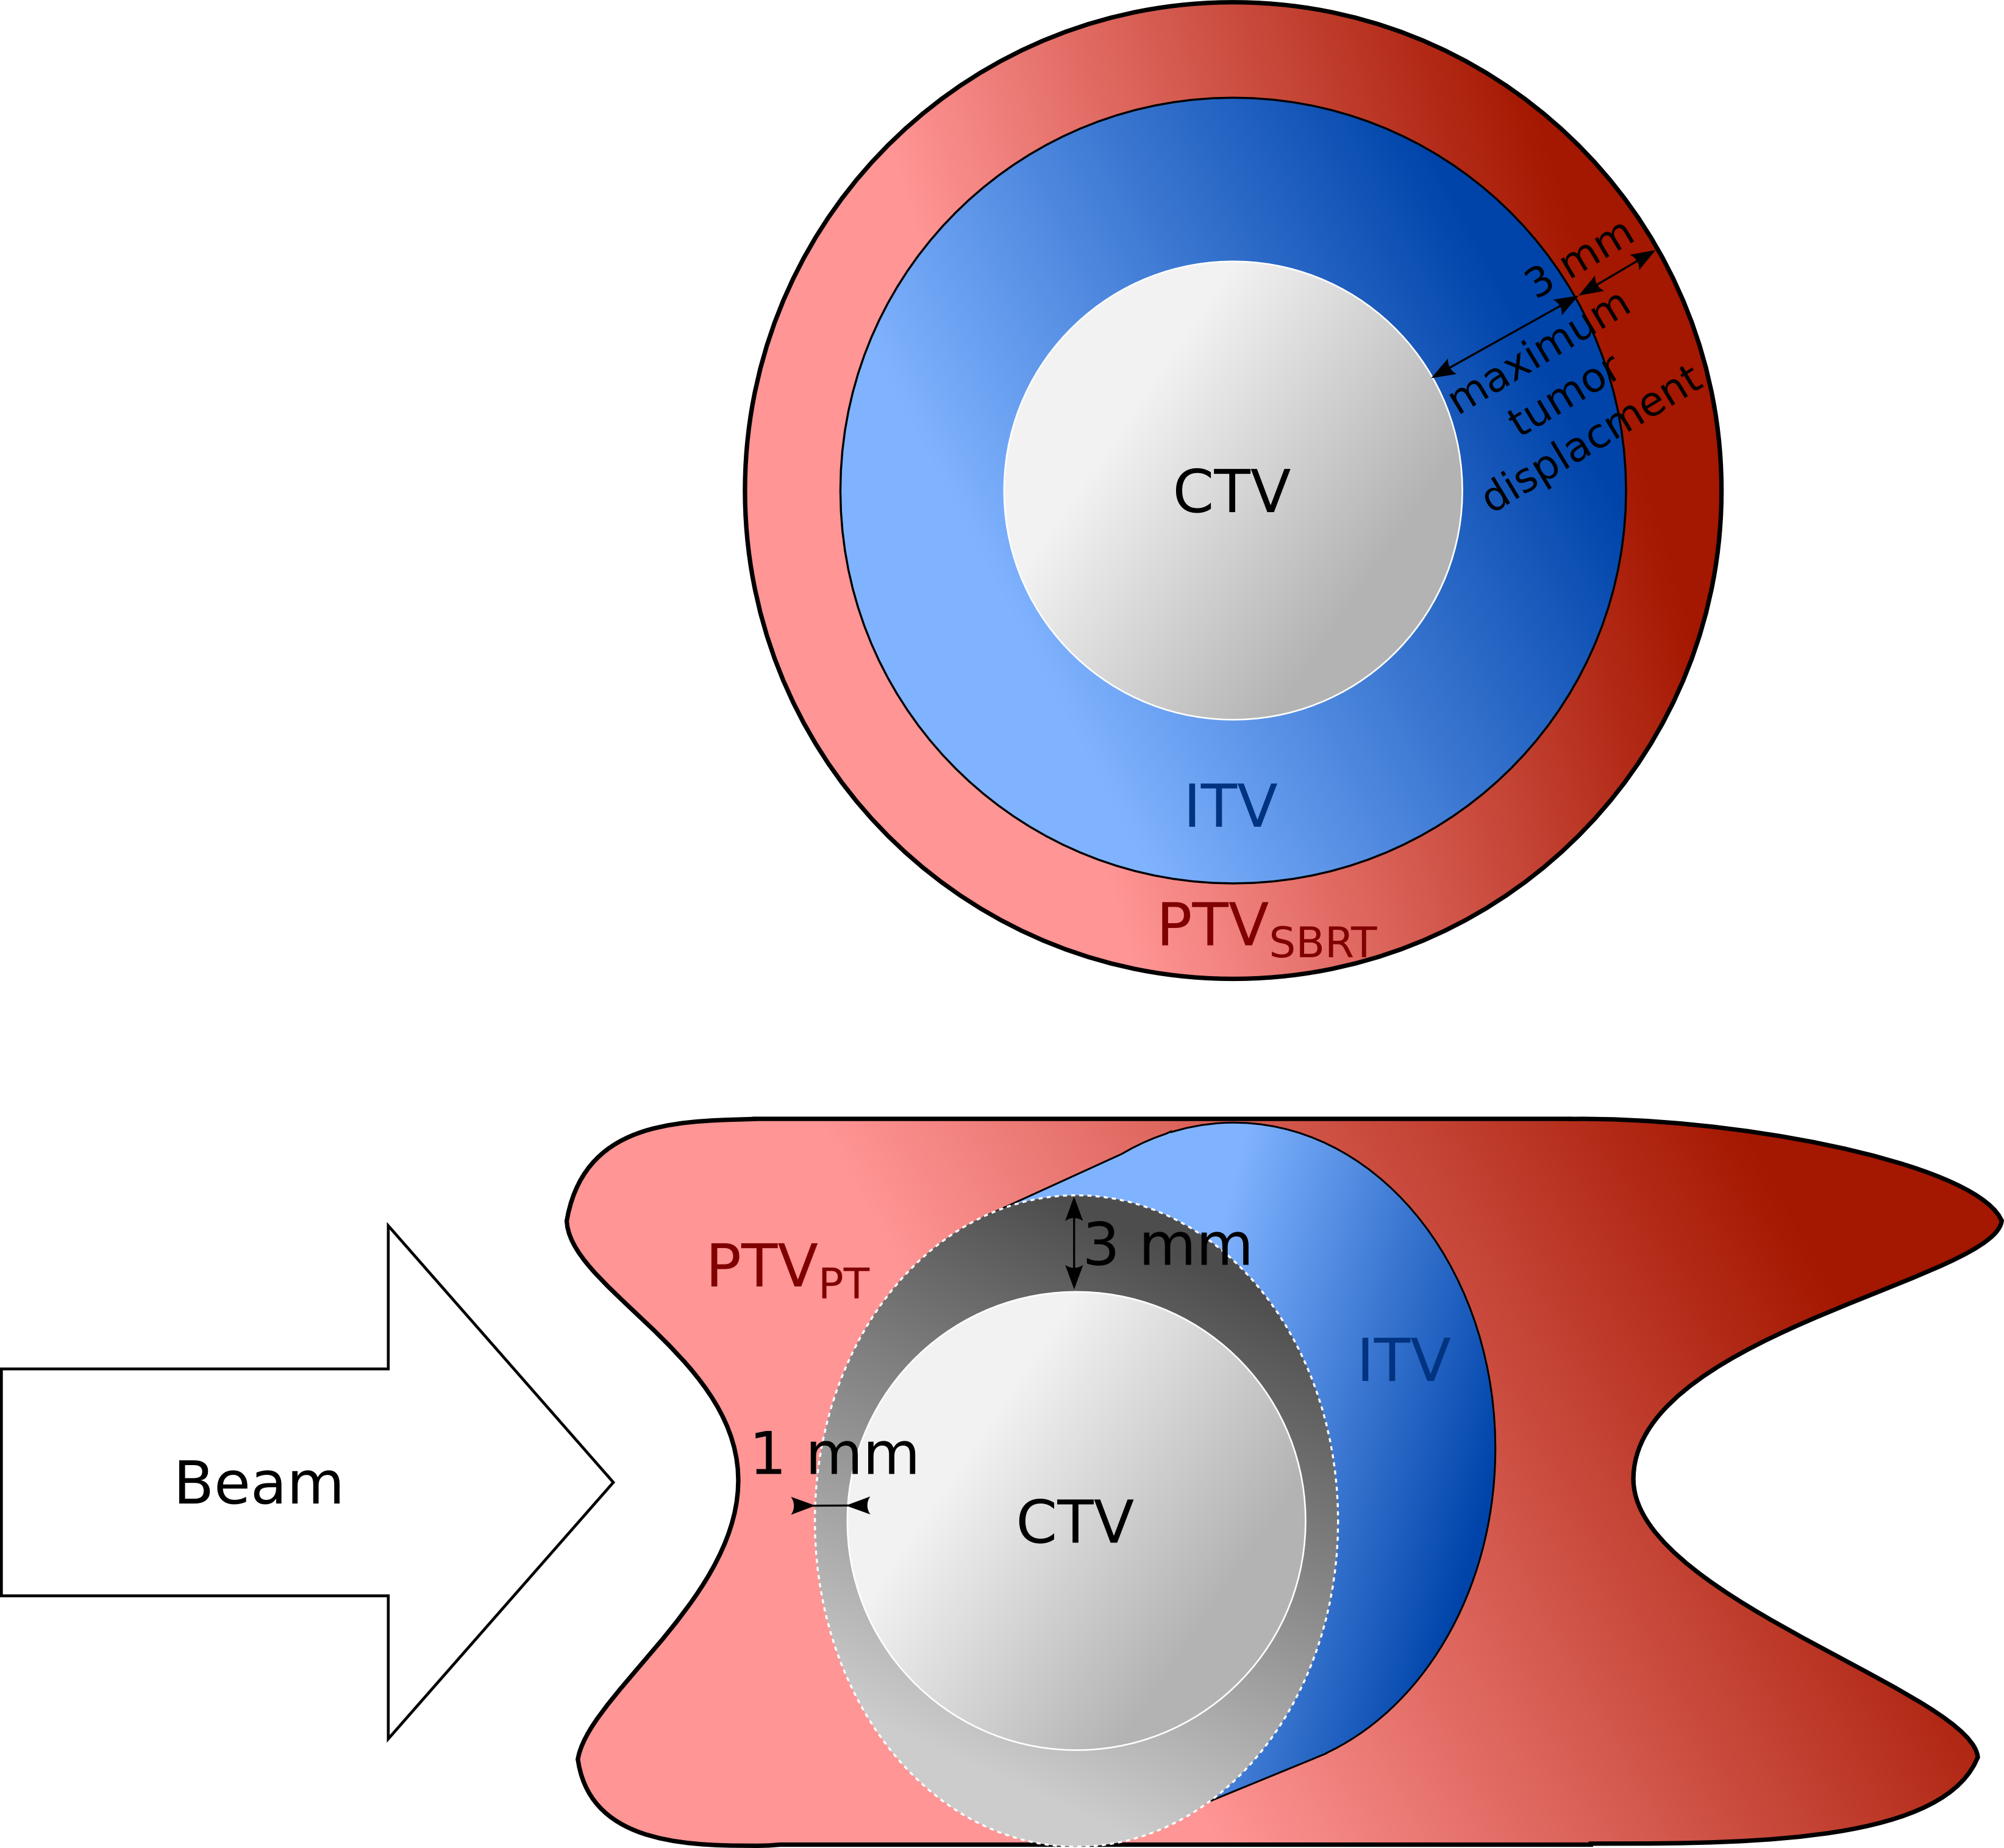
\includegraphics[width=0.8\textwidth]{./PatientStudy/Images/Figure1.png}
\caption{Different PTV definitions for SDRT (PTV$_{SBRT}$) and CiT (PTV$_{PT}$). For PTV$_{SBRT}$ isotropic margins of 3 mm plus maximum tumor displacement due to 
breathing were used on the CTV; For PTV$_{PT}$ margins of 3 mm laterally and 1 mm in beam’s eye view were used and then range-ITV was constructed with
2 mm + 2\% range margins added for PTV$_{PT}$ in end-inhale phase.}
\label{Fig:PTV_def}
\end{center}
\end{figure}

\newpage

\subsection{SDRT treatment planning}
\label{SBRTTP}

The clinical plans were calculated with the Eclipse v10 planning system (Varian Medical Systems, Palo Alto, USA) using the AAA beam model. They were all VMAT plans generally consisting of 4 overlapping partial arcs, 2 in clockwise and 2 anticlockwise direction, with a gantry range of typically 200°. For tumor sizes > 2.5 cm a calculation grid of 2.5 mm was used, otherwise this was 1 mm. During optimization, a first iteration included the PTV$_{SBRT}$ only, after which the OARs were added. In order to lower OAR dose and improve the PTV$_{SBRT}$ homogeneity, we created an artificial shell of 2 cm around the PTV$_{SBRT}$ and minimized the dose there as well. During optimization the fast Multi Resolution Dose Calculation (MRDC) model was used, with one intermediate step using the slower but more accurate AAA model to get an adequate PTV$_{SBRT}$ coverage after optimization.


\subsection{Carbon-ions treatment planning}
\label{PTTP}

For PT, state of the art 4D treatment planning software TRiP98 was used \cite{Richter2013}. A single field uniform dose plan (SFUD) 
was optimized on the PTV$_{PT}$ in the end-inhale reference phase of the 4D-CT. Most targets ($n=20$) were planned with two fields. 
For the remaining targets, one ($n=1$), three ($n=3$) or four ($n=2$) fields were used due to proximity of OARs. 
A regular grid of beam spots with a spacing of 2 mm, a beam spot full width at half maximum (FWHM) size of approximately 6 mm and a 
3 mm ripple filter were used. To compensate for short particle ranges in lung tissue, a bolus of 80 mm water-equivalent thickness 
was added.

The relative biological effectiveness (RBE) following the local effect model (LEM) IV \cite{Elsaesser2010}. 
For a conservative estimation, an alpha-beta ratio of 6 Gy and 2 Gy were used for target and OARs, respectively. 
This led to an RBE of approximately 1.1 in target tissue and approximately 1.1 to 3 in OARs.
Dose was calculated on end-inhale (3D-Dose$_{0\%}$) and end-exhale (3D-Dose$_{50\%}$) phases. 
4D dose delivery was simulated as described by Richter et al \cite{Richter2014}. Two different breathing periods (3.6 and 5 s) 
and two different starting phases (0° and 90°) were used. Simulations without motion compensation (4D-Dose$_{interplay}$)
and with slice-by-slice raster rescanning were performed (4D-Dose$_{rescan}$). Five rescans were used for the majority 
of targets (n=24), whereas 20 rescans were used for targets where the interplay effects were too big to achieve a 
satisfactory target coverage ($n=2$; lesions 3 and 18 in Table~\ref{tab:patdata}). 


%\begin{figure}[H]
%\begin{center}
%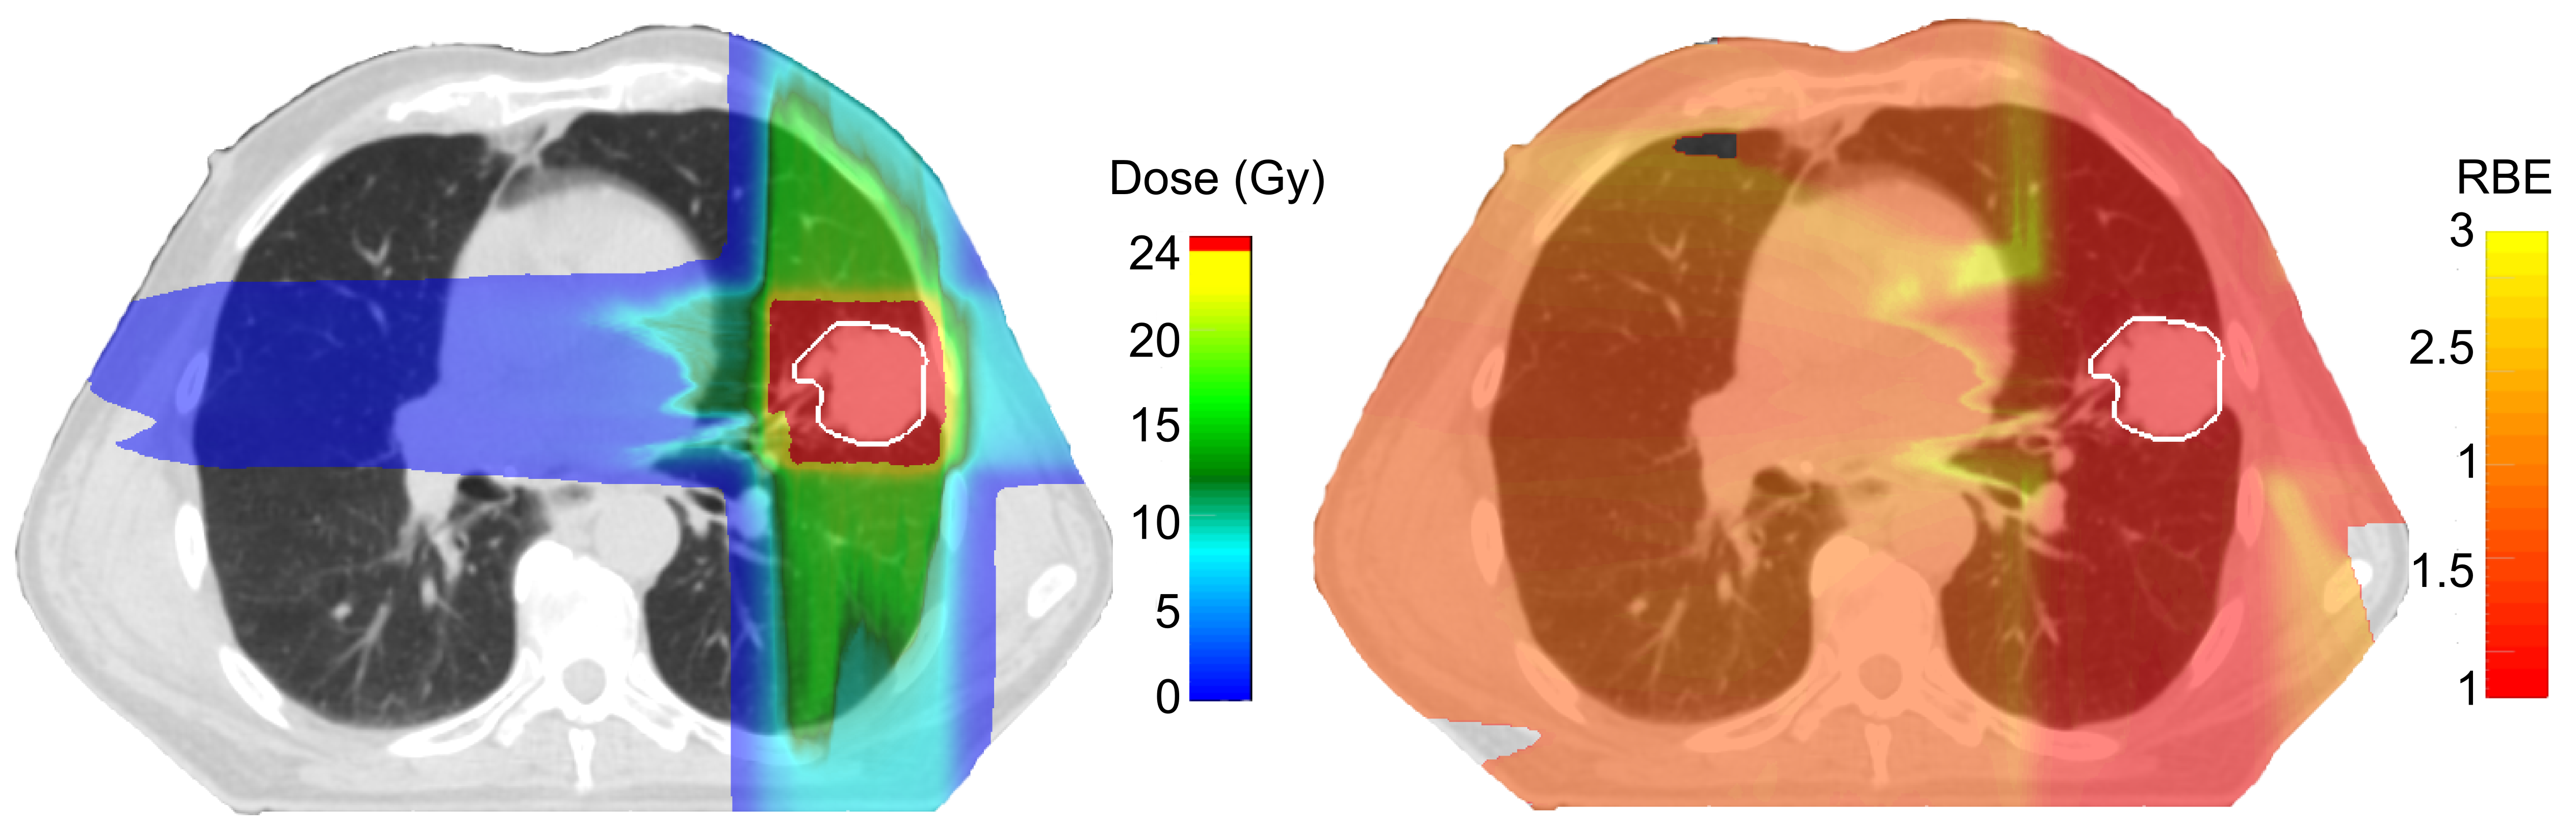
\includegraphics[width=0.9\textwidth]{./PatientStudy/Images/RBE.png}
%\caption{RBE distribution in a patient (a) depends on a actual dose profile (b).}
%\label{Fig:RBE}
%\end{center}
%\end{figure}

\subsection{Dose metrics and analysis}

For comparison between SBRT and PT the following dose metrics were used - for the target the minimum dose in 99\% of the volume ($D_{99\%}$), which should be higher than 24 Gy; for OARs, the maximum point dose ($D_{Max}$) and the mean dose ($D_{Mean}$). Additionally, the volume receiving 20\% of the planned dose ($V_{20\%}$) was used to assess differences in lung doses. In all cases, absorbed dose in Gy for SBRT was compared to biologically-equivalent dose in Gy(RBE) for PT.

Paired t-tests were performed to compare the dose metrics and for post-hoc exploratory analysis between groups a two-sided t-test with Welch correction for different variances was carried out. A p-value < 0.05 was considered significant. Dose differences are always reported such that higher dose levels for SBRT result in positive values.



\section{Results}

Examples of two SBRT and 4D-Dose$_{rescan}$ PT treatment plans are shown in Fig.~\ref{Fig:TreatmentPlans}. Patient 9 has two lesions in close proximity to the spinal cord. Patient 2 has a small lesion (1.6 cm$^{3}$) in the superior position of the left lung. $D_{99\%}$ is 100\% for SBRT and PT in all CTVs for Patient A and B; average OAR difference between SBRT and PT in $D_{Max}$ is 5.1 Gy and 1.4 Gy and in mean dose 1.4 Gy and 0.7 Gy, respectively for patient A and B.


\begin{figure}[H]
\begin{center}
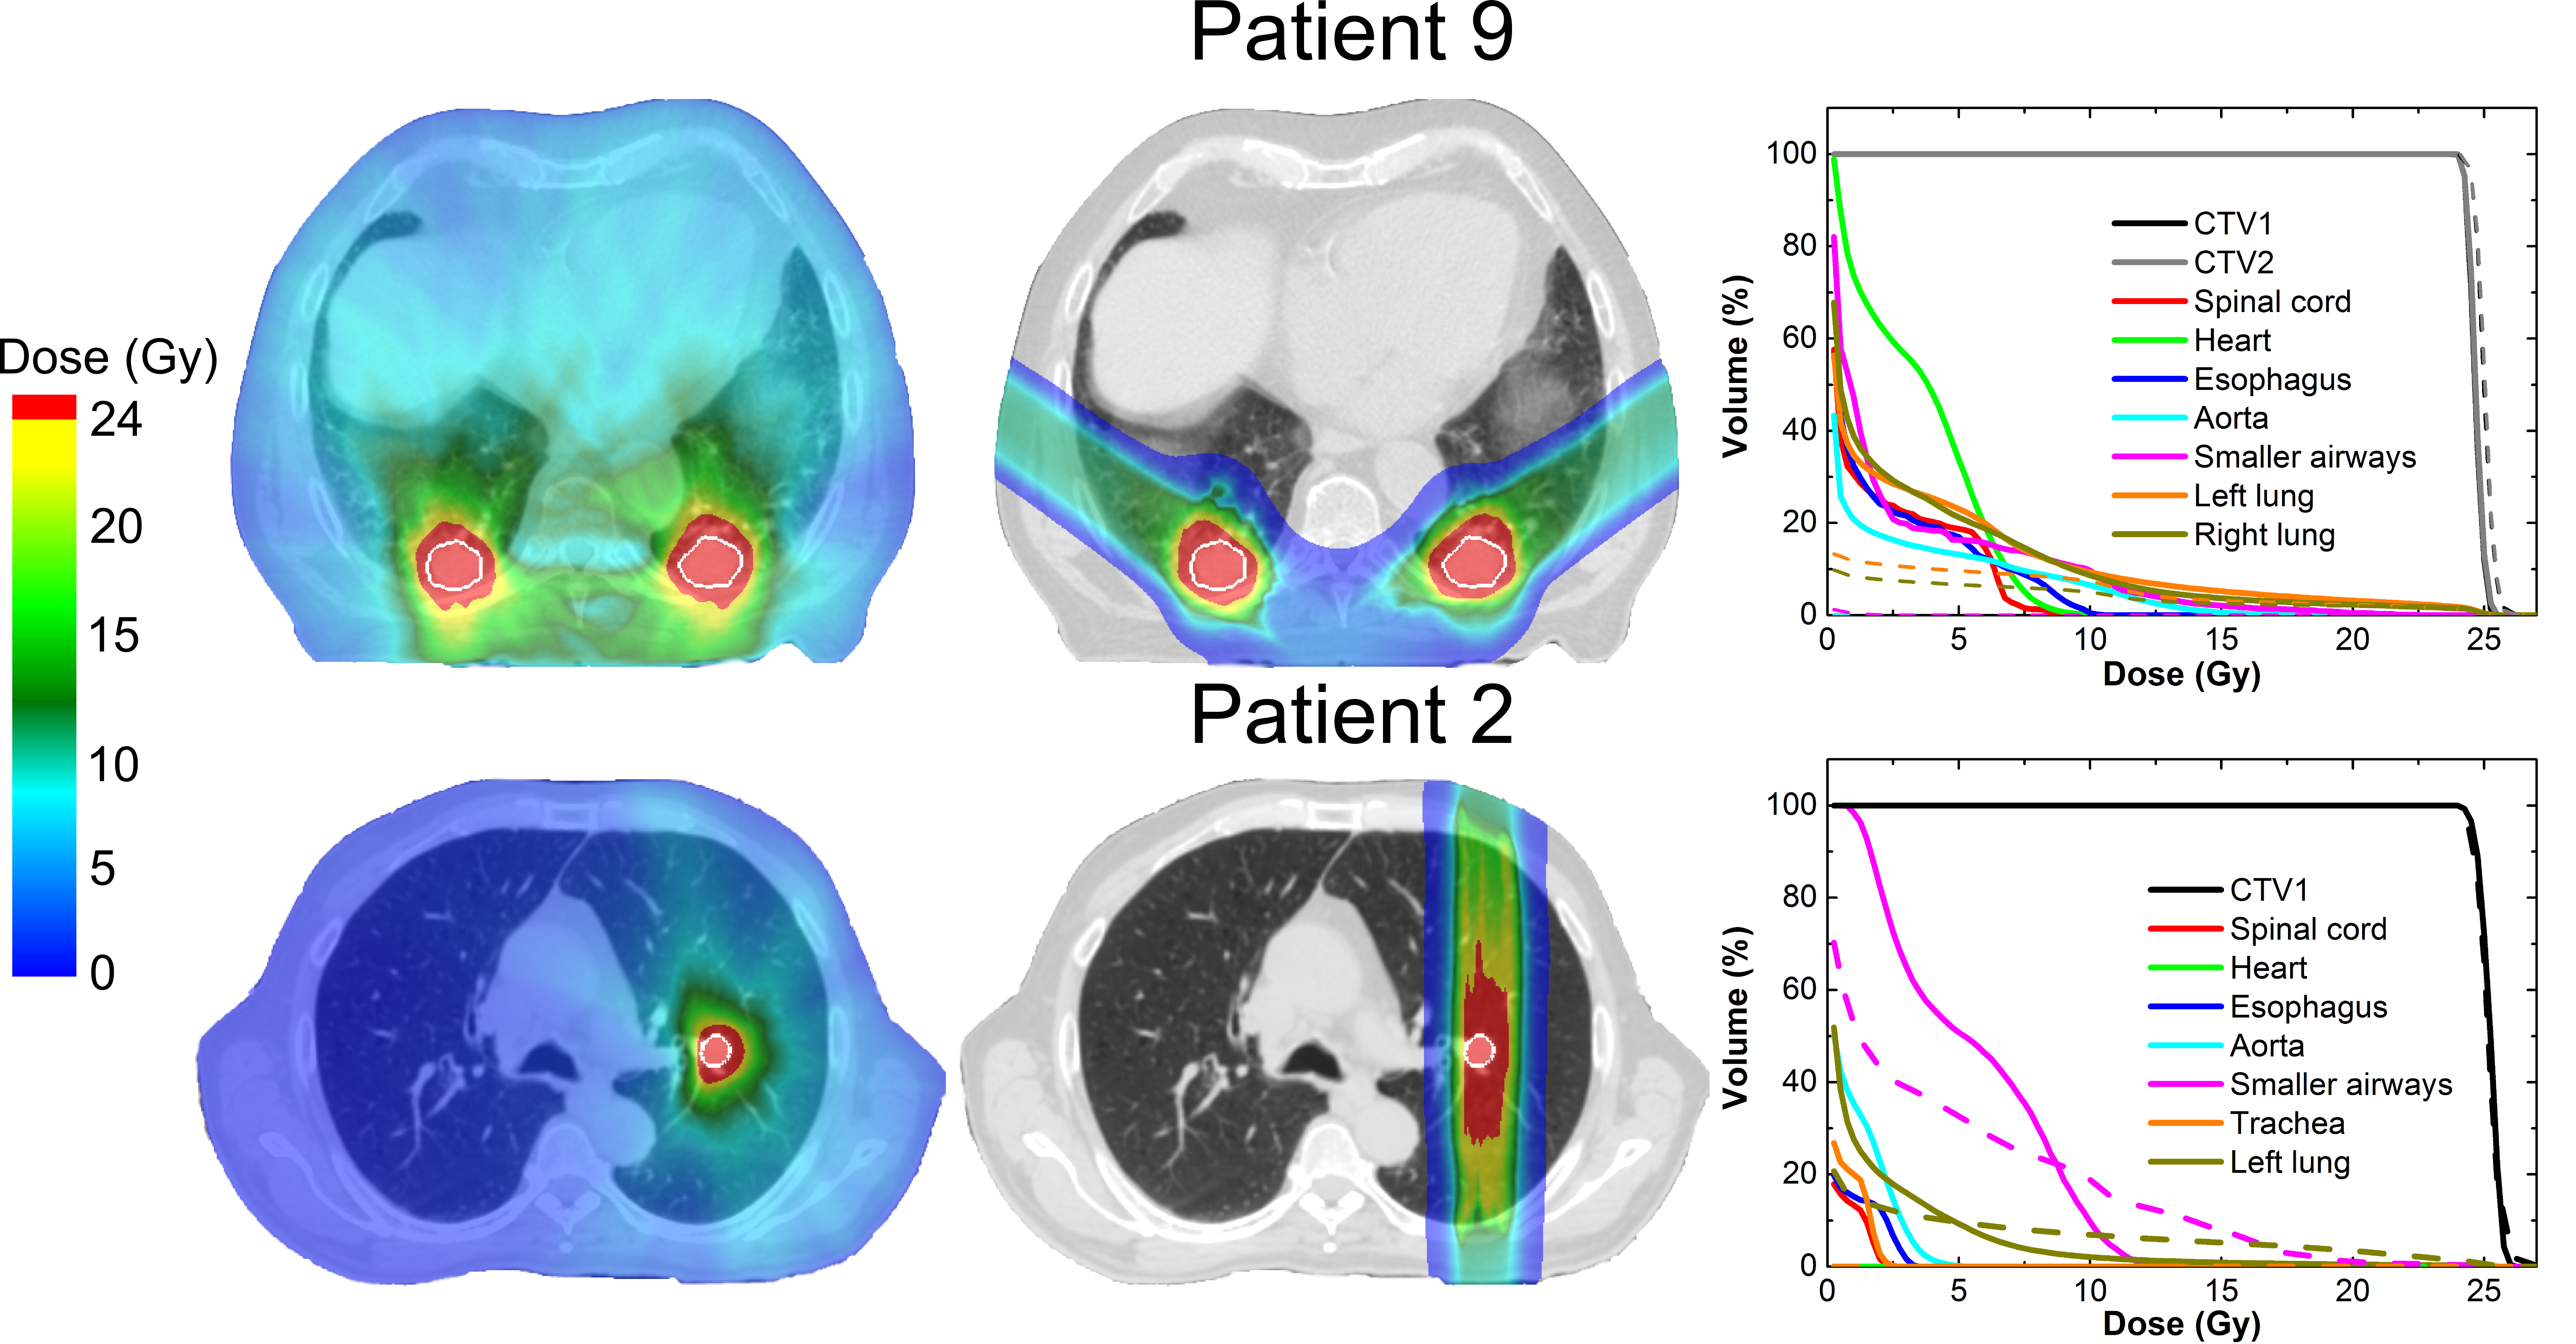
\includegraphics[width=0.9\textwidth]{./PatientStudy/Images/Figure2.png}
\caption{Treatment plans for SBRT (left), PT (middle) and dose volume histogram (right) for SBRT (solid lines) and PT (dashed lines) for two patients. PT curves for OARs without any dose are not shown. Patient 9 (top row) might be better suited for PT and patient 2 (lower row) for SBRT. Patient 2 has a small lesion (1.6 cm$^{3}$) in a central lung region, resulting in large PTV$_{PT}$ - up to 32 cm$^{3}$, compared to PTV$_{SBRT}$ 7.7 cm$^{3}$. The CTV contour is outlined in white.}
\label{Fig:TreatmentPlans}
\end{center}
\end{figure}

\subsection{Target Coverage}

Difference in PTV definition resulted in 1.5 (1.3 - 2.1) times bigger PTV$_{PT}$ than PTV$_{SBRT}$. All SBRT plans were clinically acceptable, though in one case the $D_{99\%}$ was reduced to 16.8 Gy due to proximity of an OAR. 3D-Dose$_{0\%}$ and 3D-Dose$_{50\%}$plans provided sufficient target coverage in all patients. For 4D-Dose$_{interplay}$ and 4D-Dose$_{rescan}$ there was 63\% and 2\% cases of insufficient target coverage, respectively, across all targets and different breathing patterns. Details are shown in Fig.~\ref{Fig:InterplayDiff}. For the patient with reduced dose in SBRT, PT could increase the $D_{99\%}$ from 16.8 Gy in SBRT to 20.3 Gy while adhering to OAR constraints. 


\begin{figure}[H]
\begin{center}
\includegraphics[width=0.9\textwidth]{./PatientStudy/Images/Figure3.png}
\caption{CTV $D_{99\%}$ for SBRT and different PT calculations. Four different breathing patterns are included for all targets in 4D-interplay and 4D-rescan. The dashed line shows the lower limit for clinical acceptance. One patient was an exception where lower target dose was accepted due to the proximity of a critical structure.  }
\label{Fig:InterplayDiff}
\end{center}
\end{figure}
\newpage
\subsection{Dose in OARs}


There was no significant difference in dose to OAR between the different PT dose calculations. 
The $D_{Max}$ and $D_{Mean}$ for SBRT and 4D-Dose$_{rescan}$ for OARs heart, spinal cord, smaller airway esophagus, trachea, aorta, ipsi- and contralateral lung are 
presented in Table~\ref{tab:results}.There was a significant difference in both $D_{Max}$ and $D_{Mean}$ for all OARs between SBRT and PT, with 
PT delivering less dose to OARs. Significant difference was also observed for $V_{20\%}$ for ipsilateral lung, which was 15.3\% (9.6 - 23.5) and 10.3\% (7.9 - 13.7) for SBRT and PT, 
respectively. The $V_{20\%}$ for contralateral lung was zero for almost all patients in SBRT and PT. The overall OAR difference for patients between SBRT and PT 
was significant, 2.8 Gy (1.6 - 3.7)  for $D_{Max}$ and 0.7 Gy (0.3 - 1.6) for $D_{Mean}$. 



\begin{table}[H]
  \centering
%   \footnotesize
  \caption{Dose metrics for OARs. First value at each organ is from SDRT and the second from 4D-rescan. All values are shown as median and 25-75\% in brackets.}
  \begin{tabular}{l|c|c|c|c|}
    \cline{2-5}
     & \multicolumn{2}{|c|}{$D_{Max}$ (Gy)} & \multicolumn{2}{|c|}{$D_{Mean}$ (Gy)} \\
     \hline
    \multicolumn{1}{|l|}{OAR} & Photon & Carbon & Photon & Carbon	\\
    \hline
\multicolumn{1}{|l|}{Heart} & 6.0 (0.3 - 11.6) & 0 (0 - 8.8)	& 1.3 (0.1 - 2.2) & 	0 (0 - 0.5) \\
\multicolumn{1}{|l|}{Spinal Cord} &	5.5 (3.3 - 8.5)	& 0 (0 - 0.5) &	0.7 (0.3 - 1.2) &	0 (0 - 0) \\
\multicolumn{1}{|l|}{Smaller Airways} & 13.0 (9.8 - 17.1) &	10.3 (3.3 - 19.1) &	2.8 (1.5 - 5.8) &	0.5 (0 - 2.6) \\
\multicolumn{1}{|l|}{Esophagus} & 5.8 (3.9 - 8.4) &	0 (0 - 0.3) &	1.1 (0.6 - 1.5) &	0 (0 - 0)\\
\multicolumn{1}{|l|}{Trachea} &3.9 (1.8 - 5.4) &	0 (0 - 0) &	1 (0.3 - 1.3) &	0 (0 - 0)\\
\multicolumn{1}{|l|}{Aorta} & 8.0 (5.1 - 21.9) &	3.9 (0 - 18.1) &	1.4 (0.7 - 1.6) &	0.1 (0 - 0.4)\\
\multicolumn{1}{|l|}{Ipsilateral Lung} & 26.3 (26.0 - 26.5) &	26.3 (25.8 - 26.5) &	1.9 (1.5 - 3.0) &	1.9 (1.4 - 2.5)\\
\multicolumn{1}{|l|}{Contralateral Lung} & 5.0 (3.5 - 9.6) &	0 (0 - 0.9) &	0.4 (0.2 - 0.6) &	0 (0 - 0) \\
    \hline\hline
  \end{tabular}
  \label{tab:results}
\end{table}




\subsection{Dependence on CTV Size}

Significant differences were observed between patients with a single CTV smaller ($n=8$) or larger ($n=7$) than 2.5 cm$^{3}$ for $D_{Max}$ and $D_{Mean}$, see Fig.~\ref{Fig:OAR_boxplots}. For patients with a smaller CTV, the dosimetric advantage over SBRT was on average 0.9 Gy and 0.5 Gy lower for $D_{Max}$ and $D_{Mean}$, respectively. This was associated with PTV$_{PT}$ definition - the average volume ratio between PTV$_{PT}$ and PTV$_{SBRT}$ was 2.9 (1.6 - 4.0) and 1.5 (1.3 - 1.8), for patients with CTV < 2.5 cm$^{3}$ and CTV > 2.5 cm$^{3}$, respectively.

The 4 patients with multiple lesions were excluded from this comparison. The $D_{Max}$ and $D_{Mean}$ difference were on average higher in these patients, but the number of patients was too low for statistical analysis. 


\begin{figure}[H]
\begin{center}
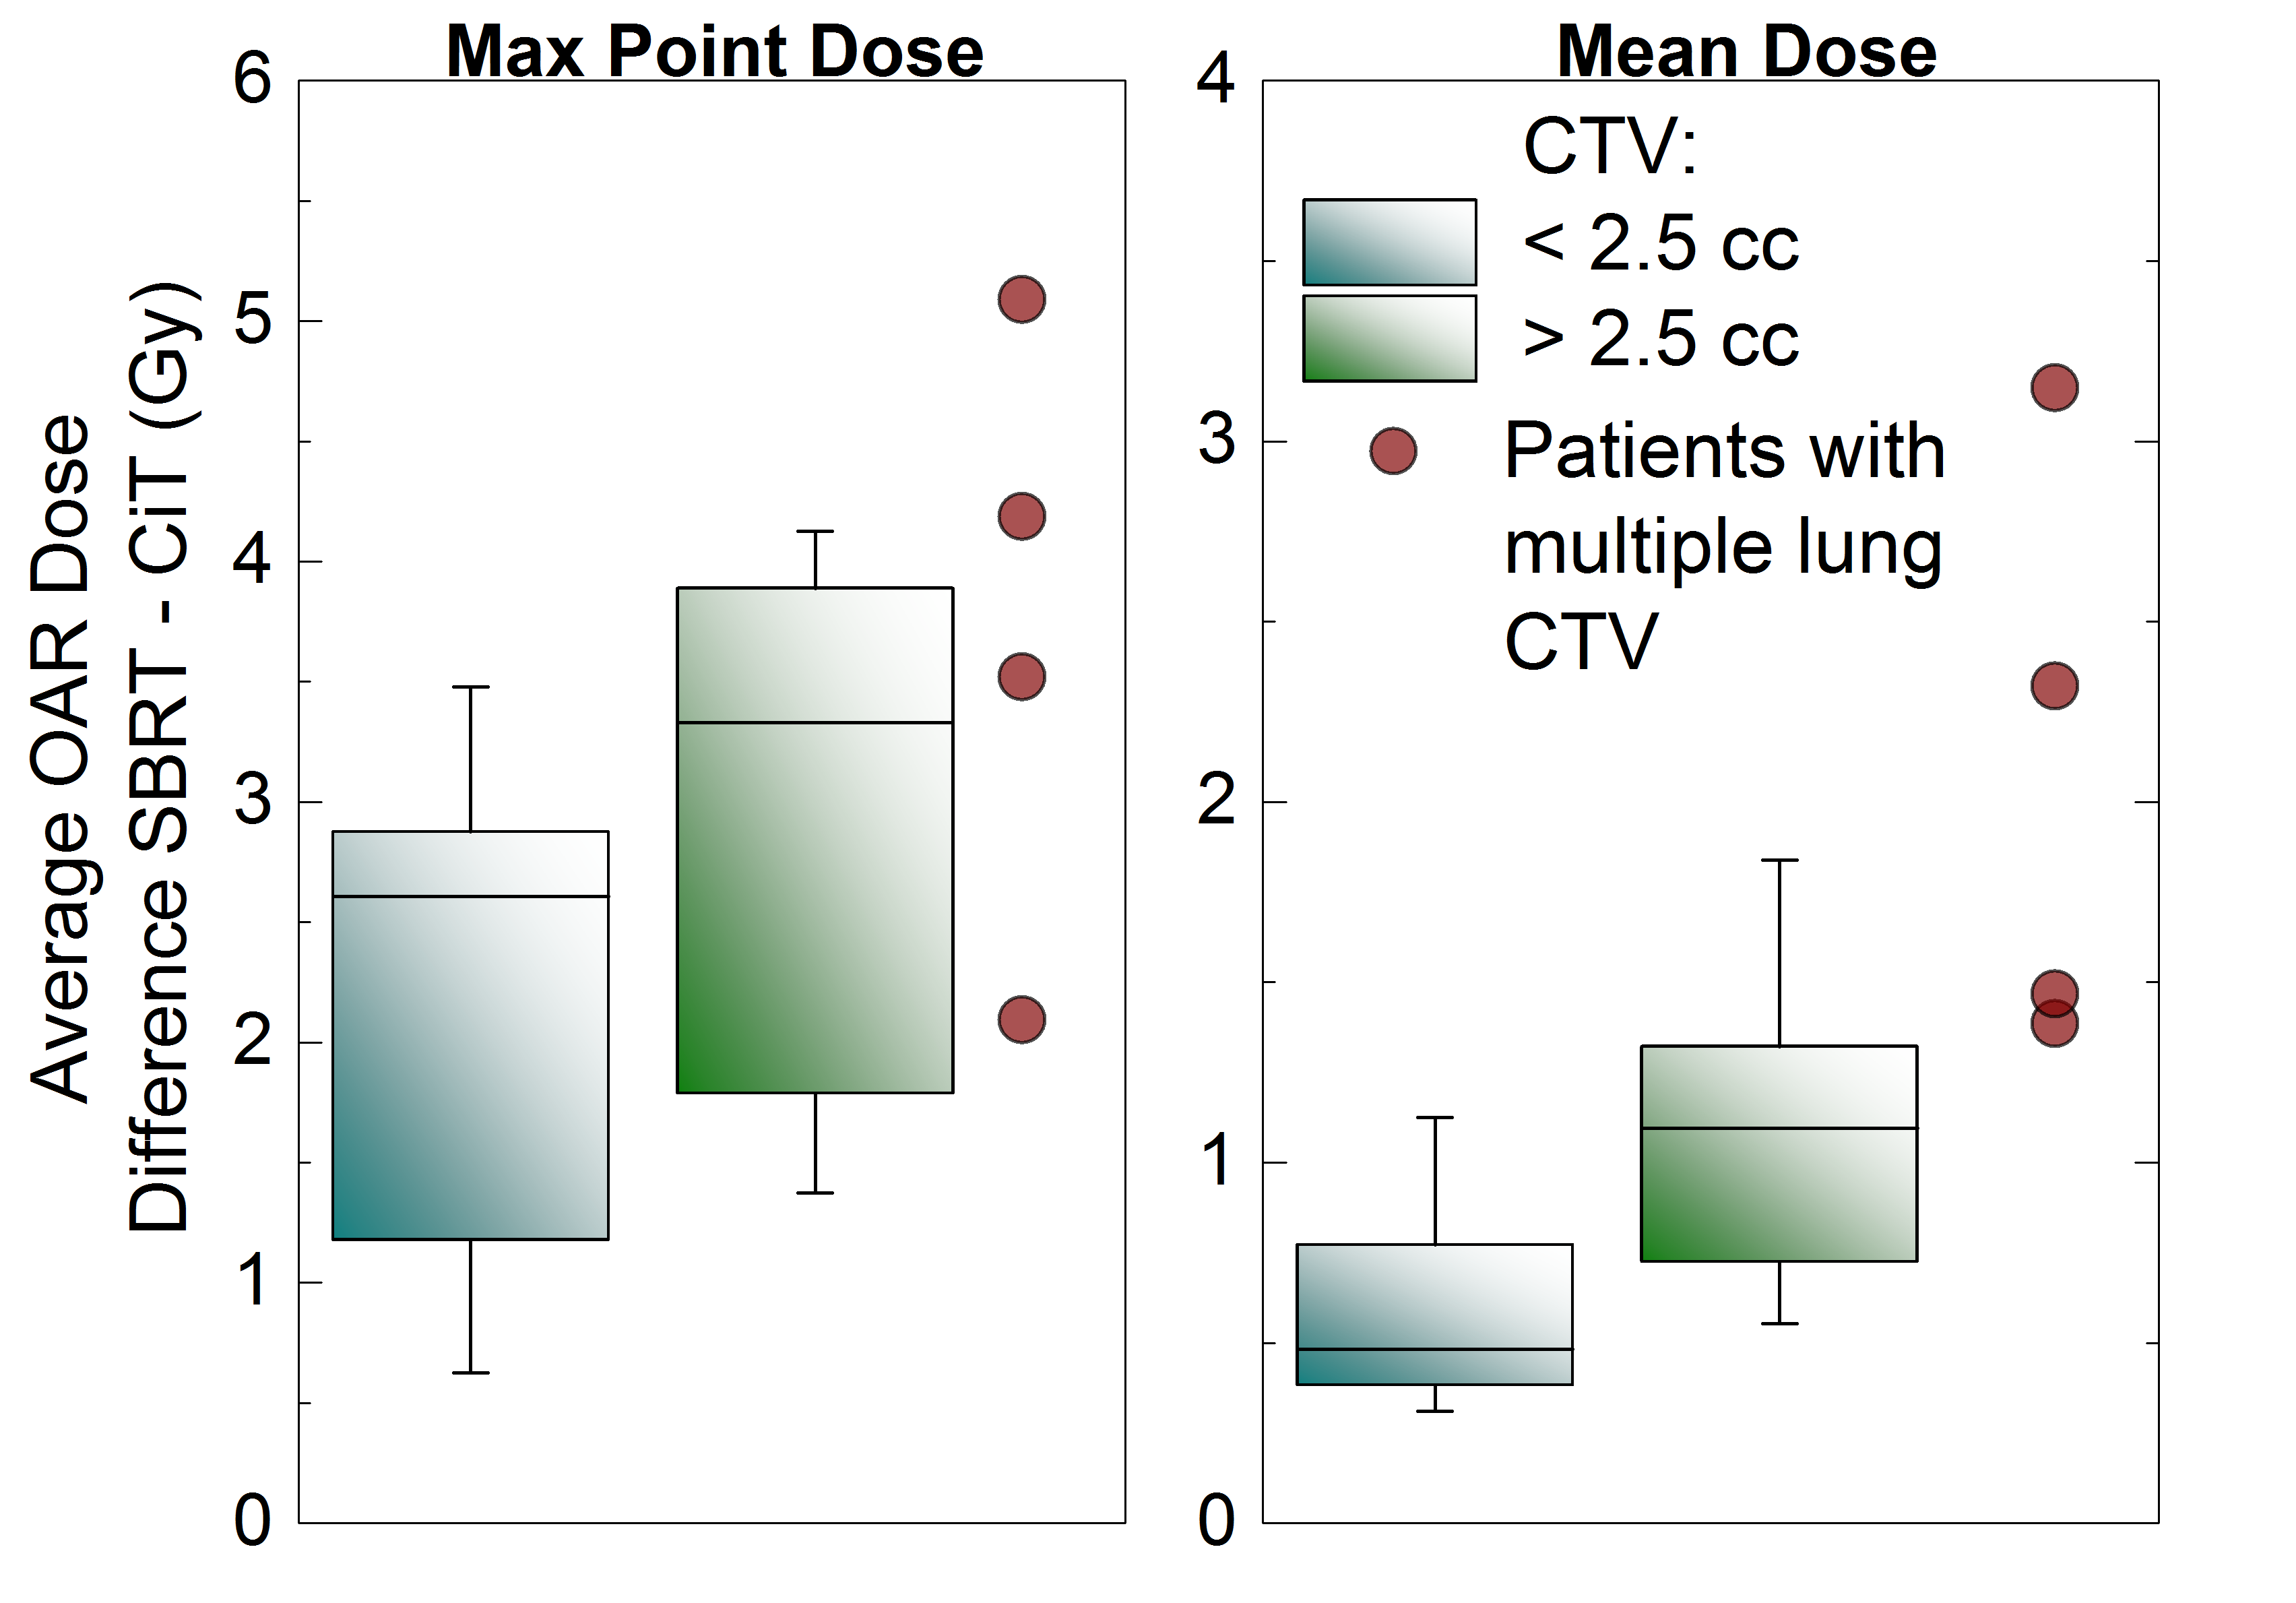
\includegraphics[width=0.9\textwidth]{./PatientStudy/Images/Figure4.png}
\caption{Box plots of average OARs max point dose ($D_{Max}$) and mean dose difference between SBRT and PT for patients with single CTV smaller ($n = 9$) or bigger ($n = 6$) than 2.5 cm$^{3}$. Boxes represent 25\% - 75\%, outliers are shown as whiskers and median is shown with solid lines. Values for patients with multiple lesions are shown with circle symbols.}
\label{Fig:OAR_boxplots}
\end{center}
\end{figure}


\section{Discussion}

This is the first in silico trial directly comparing clinically valid SBRT plans to scanned carbon ion plans using state of the art 
4D dose calculation and motion mitigation methods for NSCLC patients. Our study found that PT deposited less dose to OARs compared 
to SBRT. Therefore PT might be considered as an alternative treatment option to SBRT. The finite range of the beam permits a small 
number of fields and thus a narrow entry channel, so that critical OARs such as spinal cord, heart, esophagus, and the contralateral 
lung could be effectively spared using PT, with typically low or even zero dose. PT could be thus highly beneficial to patients with 
impaired contralateral lung function, because PT deposited no dose in the contralateral lung in 12 patients, while SBRT irradiated 
the contralateral lung in all patients. Being an intensity-modulated arc therapy, SBRT had an advantage in some patients where the 
smaller airways were in a close proximity to CTV; SBRT could shape the dose distribution to reduce dose to the smaller airways, 
compensating PT's advantageous physical dose characteristics.

Further increase in OAR sparing could be achieved by using intensity modulated particle therapy (IMPT) instead of SFUD. 
While IMPT could lead to less dose in the OARs, it would make the plans less robust against setup errors due to 
additional dose gradients between the fields. These gradients can be controlled by employing robust optimization to 
account for range, motion and setup uncertainties, which we will implement in a future 4D treatment 
planning study \cite{Chen2012, Graeff2014}.



\subsection{Range Margins and Motion Mitigation}

Since conventional geometric margins are not suitable for PT \cite{Park2012}, margins based on range changes were used. Another trial comparing photon to proton therapy in NSCLC patients also used different PTV definitions to incorporate 
range changes \cite{Roelofs2012}. As shown in our study, inclusion of range changes leads to increase in PTV$_{PT}$, up to 4.7 times compared to PTV$_{SBRT}$. 
Furthermore, the difference between PTVs is bigger for smaller tumor sizes. Patients with bigger tumor volumes (CTV > 2.5 cm$^{3}$) are therefore better suited for treatment with PT. 

Our results confirm previously published results that interplay can lead to a dose degradation in treating moving targets with active scanned beam \cite{Bert2008}. 
Figure 3 shows the importance of using 4D dose calculation and motion mitigation techniques in treating moving targets with particles. 
Even small motion amplitude can lead to underdosage in CTV without proper motion mitigation. Considering the average over the 4 simulated motion patterns, 15 patients showed a $D_{99\%}$ < 24 Gy under interplay 
conditions, as opposed to none when using rescanning (excluding the one patient with reduced target dose). Rescanning proved to be a strong mitigation technique, with robust results across all targets and different breathing patterns.

Recent studies suggest that some patients require phase-controlled layer or volumetric rescanning for sufficiently robust target coverage \cite{Mori2013,Takahashi2014}. 
The advantage of simple slice-by-slice rescanning is that no motion monitoring or assumptions on the breathing frequency are necessary \cite{Bert2011}, but the higher required number of rescans 
might increase treatment times due to reduced beam intensities. Another possibility is to combine rescanning with gating, which was already sucm$^{3}$essfully implemented in clinic \cite{Rossi2016}.




\subsection{RBE and Proton Therapy}

Carbon ions exhibit a radiobiological advantage, especially in the Bragg peak region. However, for high doses as used here the effect of RBE is not well documented and is subject to ongoing research \cite{Friedrich2014}. 
For these high doses RBE for carbon ions should approach a value between 1 and 2 \cite{Carabe2007}, which is in agreement with values in our study (around 1.1).

Coincidently, RBE values in the target at high doses are similar to those used clinically in proton therapy. Carbon-ions show considerably lower lateral scattering though, which should result in even better 
OAR sparing than protons. Our results are in agreement with several in silico studies comparing SBRT and proton therapy for NSCLC \cite{Roelofs2012, Kadoya2010, Register2010}. 
Furthermore, a study made by Kadoya reached the same conclusion as our study, that patients with larger CTV and/or multiple CTVs would  receive less dose from proton therapy \cite{Kadoya2010}.
A recent phase II trial for patients with multiple sites of extracranial disease showed good results for photons \cite{Iyengar2014}, however, based on the findings of Kadoya et al and our study, 
proton and/or carbon-ion therapy might result in even better outcome. 



\subsection{Study limitations}


The 4D dose calculations were based on a regular breathing pattern, which typically varies during patient treatment and/or between 4D-CT acquisition and actual treatment \cite{Verma2010, Malinowski2011}. 
A possible solution was proposed by Boye et al. to get motion information from 4D magnetic resonance imaging (4DMRI) and use it in 4D dose calculations \cite{Boye2013}.

Furthermore, SBRT treatment plans were done on a static case in contrast to a 4D dose calculation done for PT. This should not influence the results of our study, 
since motion has a smaller impact on photon dose distributions \cite{Zou2014}, whereas it is imperative in PT dose calculations \cite{Bert2011}. 

There were also differences in treatment planning. PT plans were done by a single person in a research setting, whereas SBRT plans were made by different people under clinical conditions with the requirement to finish the plans on time. 

Slight changes also existed between the planning CT, used for SBRT treatment plans and 4D-CT used for PT treatment plans, even though 4D-CT was usually acquired right after the planning CT. 
The propagation of contours from the planning CT to the 4D-CT and also for the 4D dose calculation rely on deformable image registration (DIR), where even small changes can effect 4D dose distribution \cite{Kashani2008}. 
Results from DIR were thoroughly checked and results were presented in Chapter~\ref{chapter:vmm}. However, the transformation of the dose with DIR is a debated topic and might jeopardize the simulated results, especially with respect to the 4D target coverage. On the other hand, dose differences 
in OARs were large and should be robust against vector field errors in the order a few mm. Nevertheless, further studies are warranted, possibly using advanced moving phantoms for an experimental 
validation \cite{Perrin2014} and finally also clinical trials. First patients are being treated in thoracic and abdominal regions with an active beam scanning at the National Institute for Radiological Sciences (NIRS) in Japan \cite{Mori2016}.



\subsection{Application}

Scanned carbon ion therapy is available only in a limited number of clinics, mainly due to the considerably higher cost in comparison to photon linacs.
Therefore a careful patient selection appears sensible. Patients with larger and multiple lesions where SDRT might be limited due to OAR constraints 
could be referred to carbon centers. In this study, already lesions larger than 2.5 cm$^3$ were found to benefit significantly stronger from CiT.

\section{Conclusion}
SBRT and PT both achieved satisfactory target dose. In most patients PT deposited less dose in all OARs (including heart, spinal cord, esophagus, trachea and aorta). Patients with multiple lesions and/or with large target volumes might be preferentially selected for particle therapy.

  
  \setcounter{mtc}{4}
  \chapter{Intensity modulated particle therapy for multiple targets}
\label{chapter:complex}
\minitoc

\section{Introduction}

Lung cancer is the leading cause of cancer-related death, with approximately 160 000 deaths in the U.S. in 2014 \cite{Siegel2014}.
More than half of all patients with lung cancer are diagnosed with stage IV non-small cell lung cancer (NSCLC) \cite{Ramalingam2008, Iyengar2014}.
Prognosis for stage IV NSCLC is poor, with only 12 months median survival after first line chemotherapy \cite{Socinski2013}. 

Stereotactic body radiation treatment (SBRT) shows good results for treating NSCLC \cite{Baumann2009, Fakiris2009, Grutters2010, Greco2011}. 
Furthermore, several studies have shown that SBRT can be used in the setting of limited metastatic 
disease \cite{Rusthoven2009, Villaruz2012, Salama2012, Iyengar2014}. 
Passive scattering particle therapy has also proved as an effective treatment for NSCLC \cite{Grutters2010, Tsujii2012} and it could be considered an alternative
to photon treatment.

It was shown in Chapter~\ref{PatStudy} that scanned carbon ions (PT) could also be used as a treatment modality for NSCLC. One of the conclusions of the study shown in Chapter~\ref{PatStudy} 
was that patients with multiple disease sites would especially benefit from PT compared to SBRT. However, limitations of this study were the small number of patients (4) and
a single-field uniform optimization (SFUD) used in treatment planning. Several vital organs need to be considered In treatment planning for NSCLC patients, besides lungs, such as heart, spinal cord, esophagus and large vessels.
Due to overlapping entry channels SFUD is limited in treating NSCLC, especially in patients with tumor in close vicinity to an vital organ.
It is not possible to create clinically acceptable treatment plans with SFUD for such complex geometry.

We hypothesize that intensity modulated particle therapy (IMPT), permits to calculate adequate treatment plans. Furthermore, IMPT 
should provide single fraction scheme in patients, where SBRT was limited by OAR constraints. 

Treatment of lung cancer patients  with multiple disease sites was investigated with state of the art 4D IMPT optimization. 
Treatment plans were generated with two different 4D optimization techniques and compared with SBRT plans, which were actually used for treating patients.


%A simple geometrical union of target contour in different CT states, geo-ITV, leads to poor 4D dose distribution, when treating moving tumors with particle therapy \cite{Rietzel2010}.
\newpage
\section{Materials and Methods}

The 4D extension of GSI's treatment planning system TRiP98 \cite{Kraemer2000a, Richter2013} was used and modified to create treatment plans. A description of modifications and tools used will be given here, 
alongside with patient data.

\subsection{Patient data}


In this study, 8 patients with 2 - 5 lung metastases summing to 24 metastases in total were included. The lesion size was 4.2 cm$^3$ (median, 25-75\% 2.4 - 22.2) and peak-to-peak motion was 5.9 mm (2.7 - 8.1). 
Details are given in Table~\ref{tab:patdata2}.
Target motion and PT treatment planning were based on a 4D-CT, consisting of 10 phases (0 - 9), with phase 0 (end-inhale) chosen as a reference phase.
A registered positron emission tomography (PET) scan was used to delineate clinical target volumes (CTV). 

Patients 1 - 3 had no while patients 4 - 8 had at least one OAR in CTV vicinity (closer than 10 mm).

Patients were treated with SBRT at Chamaplimaud Center for the Unknown, Lisbon (Portugal), with different fraction schemes. 
Number of fractions and doses delivered are given in Table~\ref{tab:patdata2}.

\newpage


\begin{table}[H]
	\centering
	%   \footnotesize
	\caption{Target characteristics, with CTV volumes, peak-to-peak motions, fractionation schemes and number of fields used for PT treatment planning. Last column 
	shows an OAR in target vicinity (closer than 10 mm), if present. SA stands for smaller airways and esoph. for esophagus.}
	\begin{tabular}{c|c|c|c|c|c|c}
		\hline\hline
		\multirow{2}{*}{Patient} & \multirow{2}{*}{Target} & \multirow{2}{*}{Volume (cm$^3$)} & Peak-to-peak & Fractionation & Number & OAR in \\
		 & & & motion [mm] & scheme & of fields & proximity \\
		\hline
		\multirow{2}{*}{1} & a & 10.2 & 3.4  & 1 x 24 Gy & 2 & \\
		 & b & 14.4 & 2.8 & 1 x 24 Gy  & 2 &  \\

		 
		 \hline
		 \multirow{5}{*}{2} & a & 3.8 & 5.8  & 1 x 24 Gy & 2 &\\
		  & b & 4.3 & 0.8  & 1 x 24 Gy& 2 &\\
		  & c & 2.7 & 3.4  & 1 x 24 Gy & 2&\\
		  & d & 3.1 & 2.1  & 1 x 24 Gy & 2&\\
		  & e & 0.5 & 0.5  & 1 x 24 Gy & 2&\\
		  \hline
		  \multirow{2}{*}{3} & a & 139 & 0.6 & 1 x 24 Gy & 3 \\
		 & b & 9.2 & 2.0  & 1 x 24 Gy & 2 \\
		 \hline
		 \multirow{2}{*}{4} & a & 4 & 9  & 3 x 9 Gy  & 5 & SA, esoph., heart \\
		 & b & 0.8 & 7.8  & 1 x 24 Gy & 2 \\
		 \hline
		 \multirow{4}{*}{5} & a & 3.4   & 5  & 1 x 24 Gy & 3 &  \\
				    & b & 2.4 & 4.4  & 1 x 24 Gy & 2 &\\
				    & c & 2.0 & 6.3  & 1 x 24 Gy& 2& Heart\\
				    & d & 2.4 & 6.4  & 1 x 24 Gy & 2 & Heart\\
		\hline	    
		\multirow{2}{*}{6} & a & 20.6 & 7.4 & 1 x 24 Gy & 4 & SA  \\
		 & b & 27.1 & 6.0  & 1 x 24 Gy &5 & SA  \\
		 
		 \hline
		 \multirow{2}{*}{7} & a & 2.3 & 12  & 1 x 24 Gy & 2 &\\
		 & \multirow{2}{*}{b} & \multirow{2}{*}{0.4} & \multirow{2}{*}{11.8}  & \multirow{2}{*}{5 x 7 Gy} & \multirow{2}{*}{5} & Heart, esoph., \\
		 & & & & & & stomach \\
		 \hline
		 \multirow{5}{*}{8} & a & 136 & 12  & 3 x 9 Gy & 2 & Heart\\
		  & b & 12.4 & 2.5  & 1 x 20 Gy & 2 &\\
		  & c & 123 & 14  & 3 x 9 Gy & 2  &Heart \\
		 & d & 80.7 & 17  & 1 x 22 Gy & 3  &\\
		 & e & 86.7 & 6.6  & 1 x 20 Gy & 3 & SA \\
		\hline\hline
	\end{tabular}
	\label{tab:patdata2}
\end{table}


\newpage

\subsection{Multiple targets}

The TRiP98 optimization works on minimizing the residual of a nonlinear equation system \cite{Kraemer2000a}. The cost function $E(N)$ for particle number $\vec{N}$ is:
\begin{equation}
\label{eq-costFunc}
 E(\vec{N}) = \sum_{i\in T} \left( D_{plan}^{i} - D_{act}^{i}(\vec{N})\right) +  \theta(D_{act}-D_{max})w_{OAR}\sum_{j\in OAR} \left( D_{act}^{i}(\vec{N}) - D_{Max} \right)
\end{equation}

For a CT voxel $i$ and $j$ in target $T$ and OAR, respectively; $ D_{plan}$, $D_{act}$ and $D_{max}$ are the planned, actual and maximum allowed dose, respectively; $\theta$ is a 
Heaviside step function and $w_{OAR}$ is an OAR specific weight.

The $D_{act}(\vec{N})$ is calculated as
\begin{equation}
 D_{act}(\vec{N}) = \sum_{k=1}^n RBE(N) c_{ik}N 
\end{equation}

The coefficient $c_{ik}$ gives the dose deposition at voxel $i$ of a pencil beam $k$, 
with $n$ being the number of pencil beams and RBE is relative biological effectiveness, calculated with the local effect model or LEM \cite{Elsaesser2010} . 

There is no restriction for the number of targets or fields in the minimizing function, so the first part of Eq.~\ref{eq-costFunc} can be expanded to:

\begin{equation}
\label{eq-multiCost}
 E(\vec{N}) = \sum_{T} \sum_{i\in T} \left( D_{plan}^{i,T} -\sum_{k=1}^n c_{ik}N\right)
\end{equation}

However, the setup of raster points in TRiP98 allowed only one target. It was therefore expanded in a way that a field was designated to a specific target, as displayed in Fig~\ref{Fig:multiTargets}. 
Raster points for each field are created only around the designated target. All fields contribute dose to all voxels in in optimization. Specifically, $k$ in Eq.~\ref{eq-multiCost} runs over all pencil beams. 
Because the optimization function was not changed, 
all TRiP98 4D functionalities could be used, as explained in the next sections.




\newpage


\begin{figure}[H]
	\begin{center}
		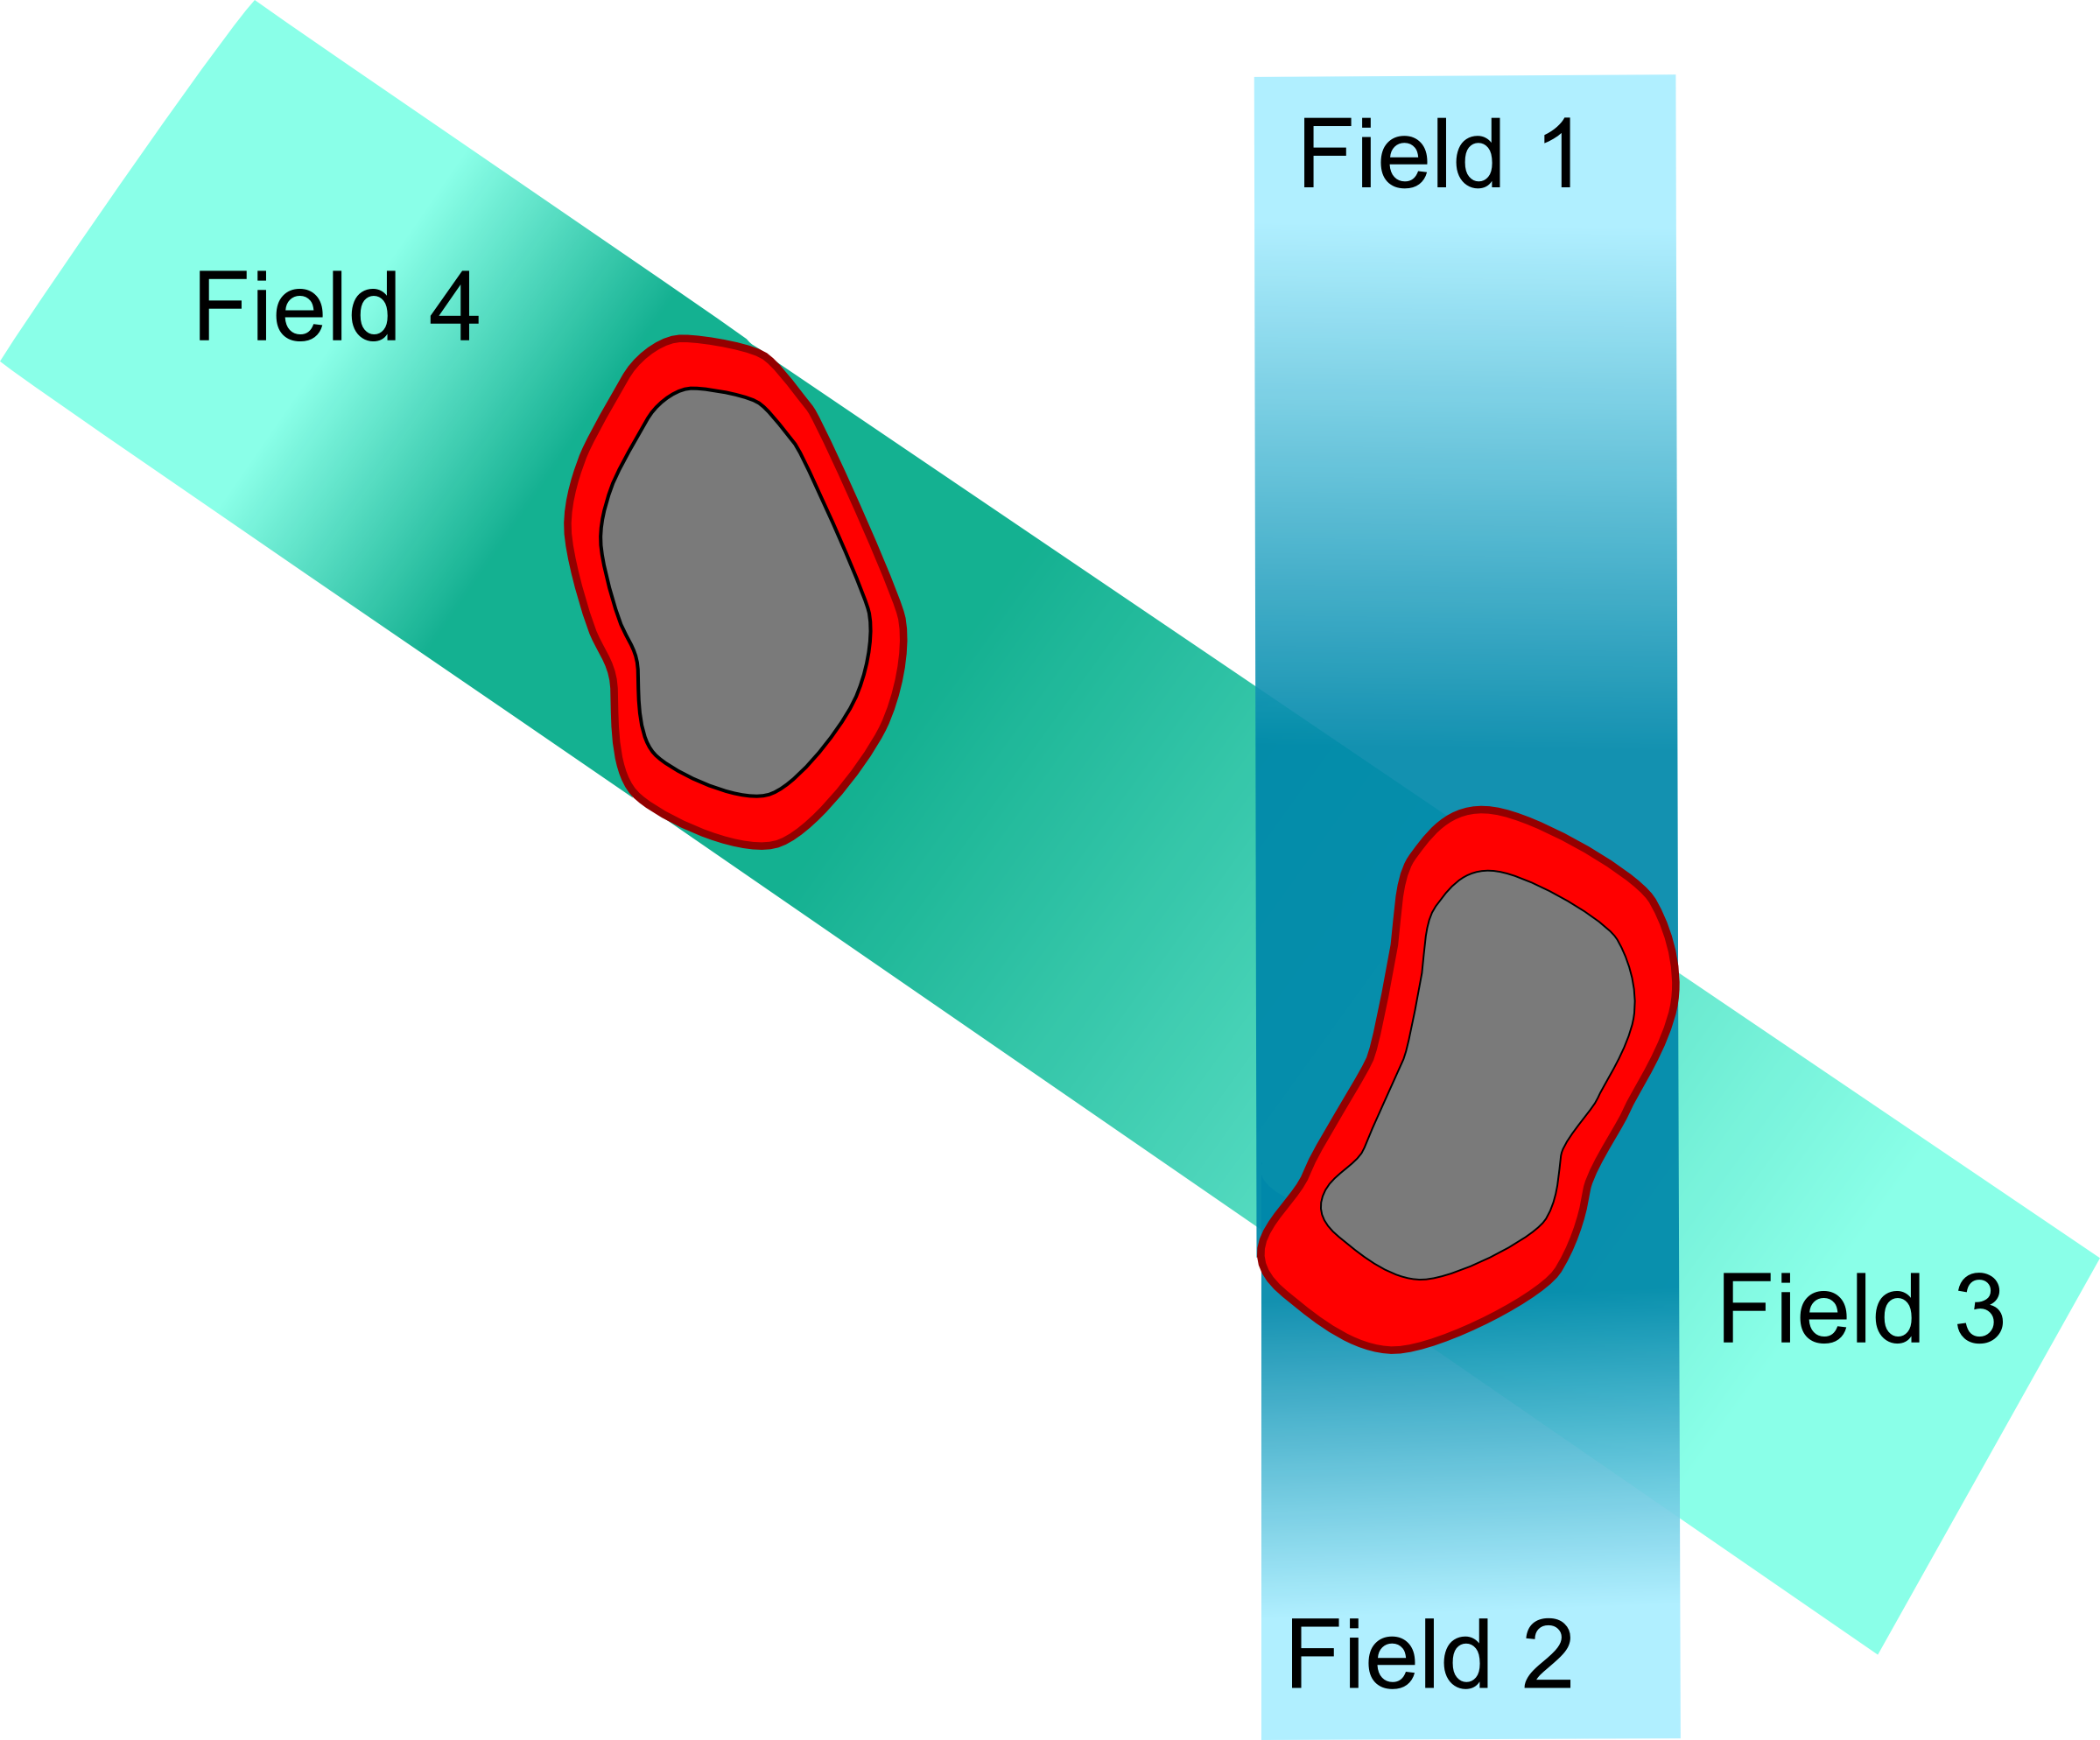
\includegraphics[width=1\textwidth]{./ComplexPatients/Images/multiTarget.png}
		\caption{Optimization of multiple targets. (a) Fields 1 and 2 are designated to target T1 and fields 3 and 4 to target T2. 
		Optimization takes into account all target voxels and contributions from all fields. An example is shown in (b) and (c), where targets
		were optimized individually (b) and together (c). The dose in (b) reaches almost 200\% in healthy tissue.}
		\label{Fig:multiTargets}
	\end{center}
\end{figure}



\subsection{Optimization techniques}

Investigation of two different optimization techniques to handle range changes in moving tumors was made. For each patient, two sets of plans were created: a field-independent ITV (ITV) and a 4D optimization (4Dopt). 

\begin{itemize}
\item \textbf{Field-independent ITV:} A water-equivalent path length ITV (WEPL-ITV) is different for each field, creating unnecessary margins when combining 
WEPL-ITV from different fields (see Fig.~\ref{Fig:weplITV}a). 
Graeff et. al \cite{Graeff2012} proposed a solution to include range margins into the field description itself, instead of creating a bigger PTV. 

Thus, all fields have the same target in optimization, permiting simultaneous optimization. 
Treatment plans were made for all targets with IMPT on a ITV in reference phase. Additionally target in motion state 5 (end-exhale) was included in optimization
to make plan more robust against range changes in different motion states.

\item \textbf{4D Optimization:} To include WEPL change specific to each motion state, a 4D optimization was used. 4Dopt uses a WEPL-ITV for raster setup, 
however the actual optimization is performed on each target voxel in each motion state $m$. The optimization function thus changes to \cite{Graeff2012}:

\begin{equation}
E(\vec{N}) = \sum_{m=1}^{M}\sum_{T_m} \sum_{i\in T_m} \left( D_{plan}^{i} -\sum_{k=1}^n c_{ikm}N\right)
\end{equation}

All targets were treated with IMPT and 4D optimization. Due to the large optimization problem for targets 3a - b, 5a - d, 6b, 8a and 8c, where targets had a big volume or 
OARs were included besides targets in optimization a subset of motion states was used \cite{Graeff2012}. 
To cover most of the different tumor positions, two extreme motion states (0 and 5) and an intermediate position (7) were chosen.

\end{itemize}

The same number of fields and the same field angles were used in both techniques.

To reduce optimization problem, only portion of large OARs, such as heart or esophagus, were used. Large OARs were manually cropped to the region close to the 
target. Dose, however, was calculated on a whole OAR to ensure the validity of results.

For targets with different fractionation scheme (targets 8a-e), TRiP98 was modified to include option of specific dose fractions for specific target.


\begin{figure}[H]
	\begin{center}
		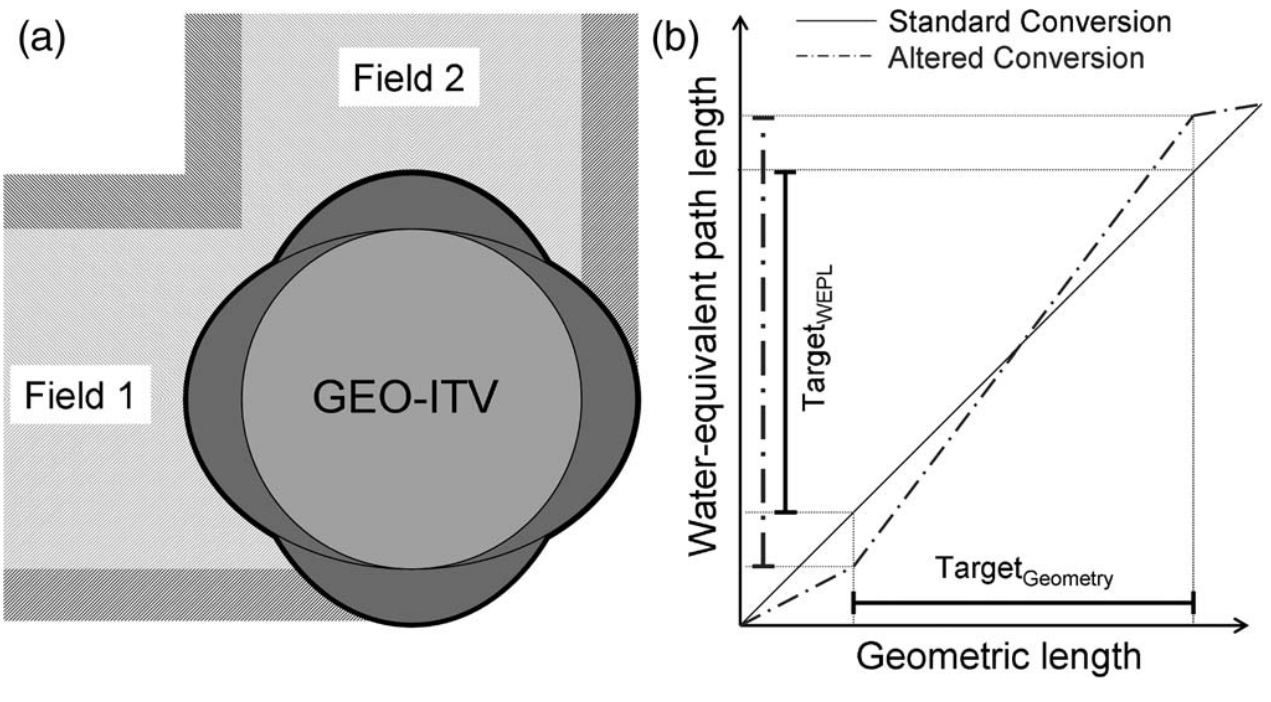
\includegraphics[width=0.7\textwidth]{./ComplexPatients/Images/weplITV.png}
		\caption{Schematic presentation of the ITV. (a) Dark gray ellipses show margins needed for specific fields to account for range changes in different motion states.
		When common target volume for two perpendicular fields is generated (this black contour) it creates unnecessary lateral extension of both fields, as shown by the dark gray
		entry channels. A solution is shown in (b). Rather than using standard, geometric margins, both fields use the same geometry, however the conversion of geometry to WEPL
		is altered for each field. The plot in (b) shows the standard (solid line) and an altered conversion (dashed-doted line) for a beam passing a homogeneous CTV. The altered conversion
		increases the WEPL extent and thus implicitly increasing margins for a single field only. Figure taken from \cite{Graeff2012}}
		\label{Fig:weplITV}
	\end{center}
\end{figure}

\subsection{Treatment planning}

An isotropic margin of 3 mm was added to each CTV to account for uncertainties in treatment delivery. 
A WEPL-ITV was constructed on the CTV with margins for each individual field, which was than used either in optimization (ITV)
or for raster setup (4Dopt). Due to large memory demands, targets in each lung were optimized separately. 
  
The planning objective was 99\% of each target volume should receive at least 100\% of the planned dose (D$_{99}$\% $\geq$ 100\%). Two dose limitation were used for OARs, as defined in 
the AAPM task group \cite{Benedict2010}. The first limitation was a maximum dose to single voxel $D_{Max}$ and the second a maximum dose deposited to a 
specific OAR volume $D_{Threshold}$. All limits are summarized in Table~appendix.
 
After the optimization the 4D-dose was calculated for two motion periods (3.6 sec and 5.0 sec) and two starting phases (0$^\circ$ and 90$^\circ$) as explained in Section~\ref{PTTP}. 
The relative biological effectiveness (RBE) was calculated with LEM IV \cite{Elsaesser2010}. 
Alpha beta ratio of 6 and 2 was used in target and normal tissue, respectively.

Motion was mitigated by applying slice-by-slice rescanning to each plan. 
The number of rescans was limited by the number of particles in a single raster point, which should not be lower than 8000 due to the
monitoring precision. The maximum number of rescanns was limited to 20.

Detailed explanation of SBRT treatment planning is given in Section~\ref{SBRTTP}.

For patients 4 - 7 OAR dose could not be sufficiently reduced in optimization. It was necessary to add margins to the OAR and then 
subtract the OAR plus margins from the target. For SBRT the OAR plus margins was subtracted from PTV, which included 3 mm isotropic margins on a geometrical ITV. 
In PT geometrical ITV was not used, so in each of 10 motion states, OAR plus margins was subtracted from CTV plus 3 mm. 

In the first try the OAR was included in optimization with different weights ($w_{OAR}$ in Eq~\ref{eq-costFunc}) and without any subtraction from target. 
If any 3D treatment plan after the optimization was acceptable, a 4D dose was calculated, 
where OAR and target dose were inspected. If the plan was rejected, the optimization was repeated but with OAR subtraction from target. 



\subsection{Dose escalation}

A single fraction of 24 Gy could not be used in SBRT treatment for targets 4a, 7b and 8a-e due to OAR dose constraints. For these targets additional 
PT plans were generated with 1 x 24 Gy fractionation scheme, in order
to estimate if PT could respect OAR constraints for these targets, while delivering 1 x 24 Gy. 

\subsection{Data evaluation}

For target coverage comparison, the minimum dose in 99\% of the target volume ($D_{99\%}$) was evaluated. $D_{Max}$ and $D_{Threshold}$ were used in OAR dose comparison. $D_{Max}$ and $D_{Threshold}$ were normalized to the respective limits
in the fractionation scheme used, see Table~appendix. Additionally, the volume receiving 20\% of the planned dose ($V_{20\%}$) was used to assess ipsilateral lung dose.

Paired t-tests were performed to compare the dose metrics mentioned between SBRT, ITV and 4Dopt. A p-value < 0.05 was considered significant. 

\section{Results}

An example of different treatment plans for three patients are shown in Fig.~\ref{Fig:multiExample}. 

\newpage
\begin{figure}[H]
	\begin{center}
		\includegraphics[width=0.9\textwidth]{./ComplexPatients/Images/multiExample.png}
		\caption{Treatment plans for ITV (left), 4Dopt (middle) and SBRT (right) for patients 2 (top), 7 (middle) and 8 (bottom). 
		CTV, heart, esophagus and stomach contours are outlined in white, red, blue and orange,
		respectively. Patient 7 image is magnified to the target 7b location. Patient 2 has 5 disease sites with no OARs in target vicinity. Patient 7 had poor target coverage
		with PT due to large target motion and OAR proximity. A 1 x 24 Gy plan could be generated for patient 8 with PT, 
		while SBRT was limited with heart dose and 2 targets were treated with 3 x 9 Gy, 2 with 1 x 20 Gy and one with 1 x 22 Gy. }
		\label{Fig:multiExample}
	\end{center}
\end{figure}
\newpage
\subsection{Target Coverage}

Results for CTV $D_{99\%}$ for all patients are shown in Table~\ref{tab:resultsComplex}. All SBRT plans were approved by a physician, 
even though the prescription dose for patients 4 - 6 was not met due to an OAR proximity. Target 7b $D_{99\%}$ for PT was below prescription and SBRT delievered full dose.
Average CTV $D_{99\%}$ was 97, 95 and 98\% for ITV, 4Dopt and SBRT, respectivelly, There was a significant difference between ITV and 4Dopt and SBRT and 4Dopt.
% Excluding patients 4 - 7, there were 1 and 5 cases (out of 128) of too low CTV dose across different
% motion types for ITV and 4Dopt, respectively. For patients 4 - 6 ITV and 4Dopt had higher CTV $D_{99\%}$ than SBRT, except for target 5c and 4a for ITV.
% The lowest CTV $D_{99\%}$ was 75\% for target 7b.

% There was no significant difference in CTV $D_{99\%}$ between SBRT, ITV and 4Dopt.

\begin{table}[H]
	\centering
	%   \footnotesize
	\caption{CTV $D_{99\%}$ for ITV, 4Dopt and SBRT for 8 patients. Results for ITV and 4Dopt are shown as median (range) across different motion types.}
	\begin{tabular}{c|c|c|c|c}
		\hline\hline
		\multirow{2}{*}{Patient} & \multirow{2}{*}{Target} & \multicolumn{3}{|c}{CTV $D_{99\%}$ (\%)}  \\
		 &  & ITV & 4Dopt & SBRT \\
		 \hline
		 
\multirow{2}{*}{1} & a & 101.0(101.0 - 101.0) & 101.0(101.0 - 101.0) & 100.0\\ 
 & b & 101.0(101.0 - 102.1) & 101.0(101.0 - 101.0) & 100.0\\ 
 \hline
\multirow{5}{*}{2} & a & 101.0(101.0 - 102.1) & 100.0(99.0 - 102.1) & 106.3\\ 
 & b & 102.1(102.1 - 102.1) & 102.1(102.1 - 102.1) & 103.1\\ 
 & c & 101.0(100.0 - 101.0) & 101.6(101.0 - 102.1) & 104.2\\ 
 & d & 102.1(101.0 - 102.1) & 102.1(102.1 - 102.1) & 107.3\\ 
 & e & 101.0(101.0 - 101.0) & 101.0(101.0 - 102.1) & 108.3\\ 
 \hline
\multirow{2}{*}{3} & a & 101.0(101.0 - 101.0) & 101.0(101.0 - 101.0) & 101.0\\ 
 & b & 98.4(97.9 - 99.0) & 97.9(97.9 - 97.9) & 102.1\\ 
 \hline
\multirow{2}{*}{4} & a & 65.3(63.9 - 69.4) & 70.4(68.5 - 72.2) & 66.7\\ 
 & b & 101.0(100.0 - 102.1) & 100.5(100.0 - 102.1) & 103.1\\ 
 \hline
\multirow{4}{*}{5} & a & 100.0(99.0 - 101.0) & 100.0(100.0 - 100.0) & 101.0\\ 
 & b & 101.6(100.0 - 102.1) & 97.9(96.9 - 99.0) & 101.0\\ 
 & c & 95.3(94.8 - 96.9) & 94.3(92.7 - 94.8) & 99.0\\ 
 & d & 99.0(97.9 - 99.0) & 99.5(99.0 - 100.0) & 94.8\\ 
 \hline
\multirow{2}{*}{6} & a & 89.1(88.5 - 90.6) & 85.4(85.4 - 87.5) & 69.8\\ 
 & b & 78.6(77.1 - 79.2) & 72.4(71.9 - 72.9) & 69.8\\ 
 \hline
\multirow{2}{*}{7} & a & 102.1(102.1 - 102.1) & 99.0(99.0 - 99.0) & 101.0\\ 
 & b & 83.9(82.1 - 85.7) & 75.0(75.0 - 75.0) & 100.0\\ 
 \hline
\multirow{5}{*}{8} & a & 100.0(100.0 - 100.9) & 99.5(99.1 - 100.9) & 105.6\\ 
 & b & 101.3(100.0 - 102.5) & 100.0(100.0 - 101.3) & 105.0\\ 
 & c & 100.0(99.1 - 100.0) & 99.5(97.2 - 100.0) & 106.5\\ 
 & d & 102.3(102.3 - 102.3) & 89.8(89.8 - 90.9) & 102.3\\ 
 & e & 102.5(102.5 - 102.5) & 91.9(91.3 - 92.5) & 101.3\\ 
 \hline

\hline\hline
	\end{tabular}
	\label{tab:resultsComplex}
\end{table}

\subsection{Dose in OARs}

$D_{Max}$ and $D_{Threshold}$ for 8 OARs are shown in Table~\ref{tab:OARComplex}. Dose volume histograms (DVH) for patients 4, 6 and 7 are shown in Fig.~\ref{Fig:dvh}.
There was a significant difference between PT and SBRT in $D_{Max}$ and $D_{Threshold}$ 
for heart, spinal cord, esophagus and aorta. No significant difference was observed for $D_{Max}$ and $D_{Threshold}$ in smaller airways.
No significant difference was observed in dose to any OAR between different motion types or between ITV and 4Dopt.
The overall OAR difference for patients between SBRT and ITV
was significant, 17 (4 - 52)\% and 27 (8 - 55)\% of OAR limits for $D_{Max}$ $D_{Threshold}$, respectivelly.
The ipsilateral lung $V_{20\%}$ was 14.5(0.0 - 48.7), 14.4(0.0 - 43.7) and 29.8 (5.8 - 89.2)\% for ITV, 4Dopt and SBRT, respectively. Both, ITV and 4DITV ipsilateral lung $V_{20\%}$ was
significantely different from SBRT.

The margins used for OAR subtraction for PT and SBRT can be found in Tableappendix.

All treatment plans exceeded the $D_{Max}$ limit for smaller airways in patients 4, 6 and 8 and for heart in patient 6. 
Additionally, SBRT esophagus and Heart $D_{Max}$ limits were exceeded in patients 4 and 8, respectively.


\begin{table}[H]
	\centering
	%   \footnotesize
	\caption{OAR $D_{Max}$, $D_{Threshold}$ and ipsilateral lung $V_{20\%}$ of all patients for ITV, 4Dopt and SBRT. There was a significant difference between PT and SBRT for all OARs, except
	smaller airways' $D_{Max}$. $D_{Max}$ and $D_{Threshold}$ doses are normalized to the corresponding OAR limits in the fractionation scheme used (see \cite{Benedict2010}). 
	Data is displayed as median (range).}
	\begin{tabular}{c|c|c|c}
		\hline\hline
		 
		OAR &  ITV & 4Dopt & SBRT \\
		\hline
		& \multicolumn{3}{c}{$D_{Max}$ (\%)}  \\
		\hline
heart        & 62.0(0.0 - 100.0) & 59.5(0.0 - 97.0) & 82.5(20.0 - 103.0)\\ 
spinalcord    & 13.0(0.0 - 48.0) & 12.0(0.0 - 55.0) & 60.0(21.0 - 79.0)\\ 
smaller airways & 72.5(0.0 - 130.0) & 71.0(0.0 - 117.0) & 72.5(0.0 - 171.0)\\ 
esophagus      & 9.0(0.0 - 79.0) & 8.0(0.0 - 99.0) & 70.5(20.0 - 101.0)\\ 
aorta         & 17.5(8.0 - 61.0) & 15.0(7.0 - 61.0) & 45.0(15.0 - 74.0)\\ 
\hline\hline
& \multicolumn{3}{c}{$D_{Threshold}$ (\%)} \\
\hline
heart & 15.5(0.0 - 59.0) & 16.0(0.0 - 53.0) & 62.5(19.0 - 98.0)\\ 
spinalcord & 11.0(0.0 - 45.0) & 10.0(0.0 - 53.0) & 66.5(28.0 - 95.0)\\ 
smaller airways & 28.0(0.0 - 97.0) & 26.5(0.0 - 89.0) & 68.5(0.0 - 99.0)\\ 
esophagus & 1.0(0.0 - 17.0) & 1.0(0.0 - 20.0) & 49.0(17.0 - 99.0)\\ 
aorta & 5.5(0.0 - 30.0) & 5.5(0.0 - 28.0) & 34.5(12.0 - 59.0)\\ 
\hline\hline
& \multicolumn{3}{c}{$V_{20\%}$ (\%)} \\
\hline
Ipsilateral lung & 14.5(0.0 - 48.7) & 14.4(0.0 - 43.7) & 29.8(5.3 - 89.2)\\ 
\hline\hline
	\end{tabular}
	\label{tab:OARComplex}
\end{table}

% \begin{table}[H]
% 	\centering
% 	%   \footnotesize
% 	\caption{$D_{Max}$ and $D_{Threshold}$ for OAR in CTV vicinity for ITV, 4Dopt and SBRT. The rightmost column shown allowed doses,
% 	as defined in \cite{Benedict2010}.}
% 	\begin{tabular}{c|c|c|c|c}
% 		\hline\hline
% 
%  \multicolumn{5}{c}{Patient 1} \\ 
% SmallerAirways & 20.6(20.5 - 21.0) & 24.8(24.5 - 25.0) & 17.5& 13.3\\ 
% Esophagus & 23.0(22.3 - 23.5) & 23.3(23.0 - 23.5) & 25.5& 15.4\\ 
% Heart & 28.0(28.0 - 28.3) & 28.1(28.0 - 28.5) & 29.3& 22\\ 
%  \multicolumn{5}{c}{Patient 4} \\ 
% Heart & 22.8(22.3 - 23.3) & 23.1(22.0 - 24.3) & 22.8& 22\\ 
%  \multicolumn{5}{c}{Patient 5} \\ 
% AirwaysSmallR & 18.4(17.5 - 19.0) & 18.8(18.5 - 19.0) & 15.3& 0\\ 
% AirwaysSmallL & 22.5(21.8 - 23.3) & 18.0(17.8 - 18.3) & 25.5& 0\\ 
%  \multicolumn{5}{c}{Patient 7} \\ 
% SmallerAirways & 21.3(21.0 - 21.8) & 20.3(19.8 - 20.3) & 16.0& 13.3\\ 
% Heart & 29.8(29.5 - 30.0) & 29.5(29.3 - 29.5) & 30.5& 22\\ 
% 
% \hline\hline
% 	\end{tabular}
% 	\label{tab:OARComplex}
% \end{table}

\newpage
\begin{figure}[H]
	\begin{center}
		\includegraphics[width=0.9\textwidth]{./ComplexPatients/Images/DVH_legend.png}
		\caption{Dose volume histograms for targets 4b, 6a, 6b and 7b with relevant OARs. SBRT, ITV and 4DITV are represented by solid, dashed and dotted line, respectively. Targets are displayed
		in grayscale, while OAR colors are shown in legend. SA stands for smaller airways.}
		\label{Fig:dvh}
	\end{center}
\end{figure}
\newpage


\subsection{Dose escalation}

With PT the 1 x 24 Gy fractionation scheme could be used for targets 8a-e, violating only $D_{Max}$ for smaller airways (180\%) and heart (110\%).
The SBRT for patient 8 was limited by heart $D_{Max}$ and $D_{Threshold}$ which were 102\% and 93\%, respectively. The SBRT delievered a mean heart dose of 
3 Gy in a single fraction (out of three), whereas PT's mean heart dose was 0.8 Gy.
The difference in the heart dose can be seen in Fig~\ref{Fig:heartDVH}.

For targets 4a and 7b the 1 x 24 Gy frascionation scheme could not be generated with PT. Either the target coverage was low (CTV $D_{99\%} < 50\%$) or 
esophagus $D_{Max}$ and additionally stomach $D_{Max}$ for target 7b were exceeded.


\begin{figure}[H]
	\begin{center}
		\includegraphics[width=0.9\textwidth]{./ComplexPatients/Images/HeartDVH.png}
		\caption{Dose volume histogram for Patient 8 heart dose. SBRT (red) plan was delievered in 3 x 9 Gy fractionation scheme. ITV
		 PT plans were generated for the same fractionation scheme (green) and with dose escalation 1 x 24 scheme (blue). Dose was normalized 
		 to $D_{Max}$ heart limit in respective fractionation scheme - 30 Gy in 3 x 9 Gy and 22 Gy in 1 x 24 Gy.}
		\label{Fig:heartDVH}
	\end{center}
\end{figure}
\newpage

\section{Summary and Discussion}

Clinically valid SBRT plans have been compared to PT treatment plans for NSCLC patients with multiple metastases. 
To the best of our knowledge, this is the first study treating multiple NSCLC metastases with IMPT. A novel approach was used to handle multiple targets and combined
with state of the art 4D IMPT treatment planning. Furthermore, 4D PT doses were calculated for different motion types. 

PT on average delivered less dose to OARs, while still having comparable target coverage to SBRT.
The most important difference was in heart dose, with $D_{Threshold}$ being on average 6 times lower in PT compared to SBRT. A recent trial, RTOG 0617, has shown,
that a higher mortality rates could be attributed to higher heart dose for NSCLC patients \cite{Bradley2015}. Furthermore, as seen in Table~\ref{tab:OARComplex}, the median
$D_{Threshold}$ for all OARs is below 30\% and $D_{Threshold}$ exceeds 90\% in only one OAR in one patient. For SBRT $D_{Threshold}$ comes close to the limit in all OARs,
except aorta. There was no need to include $D_{Threshold}$ in treatment planning, whereas it is imperative in SBRT.

For patients with complex geometry (4 - 8) PT maintained or even improved target coverage in most cases, while reducing doses to OARs.
The exception was target 7b, where CTV $D_{99\%}$ was low (84\% and 75\% for ITV and 4Dopt, respectively), due to the $D_{Max}$ constraints of esophagus and stomach.
The large motion of target 7b (11.8 mm) and small target volume (0.4 cm$^3$) contributed to a poor PT plan, whereas SBRT was able to deliver full dose to the target
and adhering to OAR constraints. This supports our claim in Chapter~\ref{PatStudy} that targets with larger volume would benefit most from PT. Furthermore, for small targets
with large motion in OAR vicinity, PT generates worse plan than SBRT. It should be noted, however, that integral doses for all OARs are still lower for PT as seen in Fig~\ref{Fig:dvh}.
The only limitation for PT is usually the OAR's $D_{Max}$.

The biggest advantage of PT could be seen in Patient 8, where the fractionation scheme could be changed to 1 x 24 Gy. 
The large total target volume of Patient 8 could be irradiated with less overall dose and hence significantly reduce dose to all OARs. Most notably, the heart dose,
which was the limitation factor for SBRT. The difference of 2 Gy mean heart dose in a single fraction is tremendous and could influence the potential outcome for the specific patient.
Again, this confirms our claim of PT benefit for large targets.
Due to the OAR constraints of targets 4a and 7b, no fractionation escalation was possible with PT. 

There was a small difference in average target coverage between ITV and 4Dopt. The most notable difference was in targets 8d and 8e, where CTV $D_{99\%}$ was 10\% lower
for 4Dopt. For this patient 4Dopt was done on a subset of 4D-CTstates, which may be inadequate due to the large motion of target 8e (17 mm). In a future study,
the number of voxels included in optimization should be reduced, without loosing any target coverage. A possible solution would be an adaptive dose grid \cite{Prall2016a}
There was no significant difference between ITV and 4Dopt in dose to OARs. 
% However, in patients 4 and 6, 4Dopt was able to achieve better target coverage. With ITV, target 4a had worse coverage than 4Dopt and delivered higher dose to 
% smaller airways (see Fig~\ref{Fig:dvh}). For patient 6, 4Dopt deposited less dose to smaller airways in addition to better target coverage.


Even though PT deposits less dose to OARs with the same or even better target coverage, there is still room for improvement in PT 4D treatment planning. 
An implementation of multi-criteria objective planning should bring even better dose distribution and bring possibility to choose between trade-offs \cite{Breedveld2007, Chen2010}. 
Additionally, multiple target optimization in PT would benefit from a shell around PT where dose would be minimized. Therefore excessive dose
in healthy tissue would be further reduced. An introduction of a shell, however, would further enlarge the optimization problem, which is big already for complex geometries 
(patient 4 - 8). As mention, it might be possible to minimize the voxel number in optimization by an adaptive grid.

In Chapter~\ref{PatStudy} additional range margins to account for range uncertainties could be used in treatment planning, due to SFUD. 
Because we did not use field specific PTVs, it was not possible to include range uncertainties in our study.
Instead of creating field specific PTVs to include range uncertainties, a solution was proposed to include uncertainties in the optimization process itself \cite{Pflugfelder2008, Unkelbach2009, Fredriksson2011, Chen2012}.
Chen et al. have implemented robust optimization in multi-criteria optimization as well \cite{Chen2012}. Furthermore, in a recent treatment planning study by Liu et al. \cite{Liu2016}
a 4D robust optimization was demonstrated, with better results over 3D robust optimization for NSCLC patients. However, only breathing starting phase was used as an uncertainty,
whereas different motion types should be considered. The disadvantage of 3D and 4D robust optimization is the enlargement of the optimization problem.

Patient 4 $D_{Max}$ esophagus dose ranged over 1.3 Gy across different motion types in 4Dopt, showing the necessity of making treatment plans robust against motion uncertainty, 
especially in the hypo-fractionated regiment. Furthermore, OAR doses that are under the limits after optimization, may exceed them after calculating 4D dose. 
The ITV and 4Dopt approaches take into account range changes in different motion states, however they do not address interplay. 
This could be solved with a complete 4D optimization \cite{Graeff2013}, where a 4D raster treatment plan is 
generated and each motion state has a designated treatment plan. 

% Clinical application of beam tracking is not yet feasible due to several reasons, such as the 
% inverse interplay, the ion-beam tracking system complexity, precision and speed of the motion monitoring.
% Another solution would be jet-ventilation \cite{Santiago2013}, however, it brings additional complications to treatment.

Apart from 4D robust optimization, the effect of motion could be minimized by using other motion mitigation techniques, such as gating. Furthermore, gating could improve the target coverage, where the planned dose was
not met. Gating, together with rescanning, has already been successfully implemented clinically for active beam scanning \cite{Rossi2016, Mori2016} and it might be essential to use it in hypo-fractionated 
treatment of moving tumors \cite{Richter2014}.

A recent review showed good local control rates between 66 - 92\% for patients treated with SBRT for in-field recurrent tumors \cite{Amini2014}. 
However, there were grade 4 and 5 complications present, i.e. a study by Trovo et al.showed grade 5 pneumonia in
6\% of patients treated \cite{Trovo2014}. As shown in our study, PT delivers less dose to the OARs, ipsilateral lung in particular, and could hence reduce the number of treatment-related
complications.

\section{Conclusions}

PT delivers less dose to OARs compared to SBRT in NSCLC patients with multiple disease sites, while maintaining target coverage. Patient with large total target volume 
could be irradiated with 1 x 24 Gy, whereas it could not with SBRT. 
There was a small difference between the two 4D treatment planning techniques.

Patients with multiple NSCLC disease site have a poor prognosis, with a median survival shorther than a year. 
Treatment with SBRT can prolong a patient life, however there is a 10\% chance of death due to the severity of the treatment. PT could
maintain the SBRT survival rate, while tremendously reducing treatment related side effects.
  
  \setcounter{mtc}{5}
  \chapter{Discussion}

This is a first in silico study directly comparing clinical stereotactic body radiation therapy (SBRT) with scanned carbon-ions (PT) treatment plans for non-small cell lung cancer (NSCLC). 
Our results show, that carbon-ions could be considered an alternative to SBRT, with the same tumor coverage and less dose to OAR.

Since PT offers a precise dose shaping, it can be more prone to uncertainties and a special consideration must be paid to them. Calculation of time-resolved (4D) doses can be significantly
affected by errors in deformable image registration (DIR) \textbf{Citat}. Special tools were developed in the scope of this thesis to ensure DIR quality assurance (DIRQA). Additionally, DIRQA
was tested on a large dataset for a tool verification. Treatment of NSCLC with PT is also influenced by interplay between tumor motion and beam scanning. It was shown that rescanning offers an
adequate motion mitigation. Additionally, a prospect for treating patients with multiple lung metastases was displayed.

\section{Deformable image registration}


With features such as adaptive treatment planning \cite{Yan1997}, 4D optimization \cite{Trofimov2005}, 4D dose calculation \cite{Flampouri2006}, contour propagation \cite{Lu2006b} and
combining different imaging modalities \cite{Leibfarth2013} DIR is slowly entering everyday clinical work-flow. There are various different registration algorithms available \cite{Varadhan2013}
along with different optimization metrics, such as mean square error, cross-correlation, or normalized mutual information \cite{Glocker2011}.

The advantage of using open-source software for DIR, as explained in Section~\ref{RegistrationImplement}, is that different DIR algorithms, optimization metrics and image types can be used. Either with using
existing libraries, such as ITK \cite{Yoo2002}, or by writing designated software \cite{Fedorov2015}. A B-Spline algorithm was used for DIR in this thesis. There are large deformations present in lung and cardiac
4D-CT, which B-Spline should handle well \cite{Tang2013}. The mean square error metric also gives better results for images of the same modality and same contrast \cite{Varadhan2013}. 
The comparison between different algorithms and optimization metrics is beyond the scope of this thesis.

\subsection{Deformable image registration validation}

Any DIR algorithm must undergo thorough evaluation before it can be used clinically. The most common practice for DIRQA is visual validation \cite{Stanley2013}. Our DIRQA module offers false color, checkerboard and landmarks distance as
visual validation methods. Contour validation is currently lacking in our DIRQA module. In literature many different attempts have been done to asses DIRQA with landmarks or contours. A study by Hardcastle et al \cite{Hardcastle2012} 
compared demons and Salient-Feature-Based registration with dice coefficient between propagated and physician drawn contours.
A multi-institutional study by Brock et al \cite{Brock2010} compared differences in propagated and oncologist drawn landmarks. A method has been developed by Castillo et al \cite{Castillo2009} to automatically identify landmark points
in lung patients images. However, visual based evaluations are limited in regions of uniform image intensity and by the number of the objects being tracked \cite{Kashani2008, Liu2012}. An example of visual validation disadvantage could be seen in
pig cardiac 4D-CT, where visual evaluation did not show any errors in DIR, but errors were observed in vector fields resulting from DIR.

An alternative to visual validation is to evaluate mathematical properties of vector fields. The two most common DIR vector fields evaluation metrics are Jacobian determinant (Jacobian) and inverse consistency error (ICE) \cite{Leow2007, Christensen2001},
which we also implemented. We have shown that bigger deformations yield more deviations in Jacobian and ICE, which was also found by Stanley et al \cite{Stanley2013}. Furthermore, we have confirmed
that Jacobian should always be positive for a successful DIR \cite{Rey2002}. Additionally, our results show that ICE should be smaller than maximum vector field magnitudes. Any deviation from this checks should be thoroughly examined.

There are additional vector fields validation methods beside Jacobian and ICE, such as vector field curl \cite{Schreibmann2012}, unbalanced energy \cite{Zhong2007}, permutation and analysis of variance (ANOVA) tests \cite{Klein2009}.
It was demonstrated in a study by Salguero et al that DIR errors greater than 1 mm can lead to large dose errors in high-dose gradient regions. Therefore the DIR accuracy has to be quantified at each image voxel in the high-dose 
gradient regions. A solution to evaluate at each specific voxel and for patient-specific registration was given by Stanley at al \cite{Stanley2013}. They proposed a computational phantoms and their deformations with a finite element module framework. 

\newpage
\section{Radiation treatment for non-small cell lung cancer}

\subsection{Non-small cell lung cancer early stage}

Surgery is the gold standard in treating NSCLC in the early stages \cite{Roesch2014}. In recent years, however, SBRT showed similar results as surgery and SBRT is recommended for all high-risk surgical patients. In a recent comparison study by Yu et al \cite{Yu2015},
SBRT had lower intermediate mortality and toxicity, compared to surgery. However, patients with long life expectancies were found to benefit more from surgery. 

There are several clinical scenarios where use of SBRT might be limited. This include treatment of centrally located tumors, tumors close to chest wall, large tumors (radius > 5 cm) and multiple primary tumors \cite{Timmerman2006, Georg2008, Westover2012}.
The limitation of SBRT could open possibilities to other treatment modalities, such as particle therapy. Interestingly, two of the mentioned scenarios, large tumors and multiple tumors, would benefit the most from particle therapy, according to the results shown
in this thesis and to the results published by Kadoya et al \cite{Kadoya2010}. In a study done at Francis H. Burr Proton Therapy Center patients who could not be treated with SBRT, due to the scenarios mentioned, were treated with passive proton beam in 3 - 5 fractions, 
delivering 42 - 50 Gy \cite{Westover2012}. They observed similar tumor local control rates as in SBRT (100\% in a two year follow-up) with limited toxicities. It should be noted, that the patients treated were rejected from SBRT treatment.


\subsection{Non-small cell lung cancer advanced stage}

While treatment for early stage NSCLC is well established, more than 75\% NSCLC cases present themselves in an advance stage \cite{Jemal2009}, usually due to the lack of detection in the early stages. The standard of care for advanced NSCLC is concurrent chemotherapy \cite{Oshiro2014}.
Dose escalation studies showed favorable prognosis for doses higher than 70 Gy \cite{Hayman2001, Rosenman2002, Socinski2008}. The results of recent phase 3 randomized trial by Bradley et al \cite{Bradley2010}, however, showed better survival rates for patients delivered 60 Gy,
instead of 74 Gy. It was speculated that higher doses to heart and esophagus might have contributed to higher mortality rates for patients who were administered higher doses \cite{Cox2012}. Results presented in this thesis show that mean dose to heart and esophagus would be on average 1 Gy
smaller with PT than with SBRT. Similar results were observed when comparing protons to SBRT \cite{Georg2008}. 

In recent phase II study by Iyengar et al \cite{Iyengar2014} they treated stage IV NSCLC with SBRT and chemotherapy. They have irradiated 52 targets in 24 patients, 16 of them had more than one target. The results were promising, with 20 months median overall survival, 
compared to 9 months when treating with chemotherapy only \cite{Tsao2008}. Results in this thesis show, that patients with multiple sites would especially benefit from PT. Based on the poor prognosis that stage IV NSCLC patients have and on the results published by Iyengar et at,
stage IV NSCLC patients could be eligible candidates for PT treatment. Additionally, such patients usually exhibit chronic obstructive pulmonary disease and less dose to lung is warranted \cite{Westover2012}. This further supports our claim, since our study showed substantial differences in 
doses to ipsilateral lung ($V_{20\%}$ was on average 5\% smaller for PT) and contralateral lung as well - 70\% of patients did not receive any dose to contralateral lung, whereas SBRT deposited dose in contralateral lung in all patients.
The PT treatment planning for patients with complex geometry has to include 4D optimization and dose calculation as shown within this thesis. The treatment plan after optimization can respect the
OAR dose limits, while 4D dose can exceed them. Beam tracking \cite{Bert2007} or jet-ventilation \cite{Santiago2013} would be possible solutions, however, they significantly complicate treatment.

The results of multi-institutional randomized trial, comparing photons and particle therapy in treating NSCLC, will have an important impact on treating NSCLC \cite{RTOG1308}. 
The trial started in 2014 and we can not expect results before 2020.

\subsection{Motion mitigation}

While tumor motion influences photon treatment, the effects are not strong \cite{Zou2014}. On the other hand, effects can be substantial when treating moving targets with scanned particle therapy \cite{Bert2008}.
It was shown in this thesis that rescanning is an adequate motion mitigation technique. \textbf{Citat protoni iz predavanja}. However, rescanning has a level of uncertanity, especially regarding maximum allowed point dose to OAR.
In hypofractionated treatment this limits are strict and exact dose to OAR must be known. A possible solution would be to simulate rescanning and 4D delivery in optimization process itself. 
Gating
Tracking



\subsection{Outlook}


4pi
adaptive




RBE

24Gy(RBE) %http://www.sciencedirect.com/science/article/pii/S0360301615005179

Hypo-fractionation of liver cancer %http://ro-journal.biomedcentral.com/articles/10.1186/1748-717X-8-59  http://jco.ascopubs.org/content/early/2015/12/11/JCO.2015.64.2710.short

Future SBRT - 4pi %https://www.aapm.org/meetings/2014SS/documents/FUTUREOFSBRT2014Kupelian.pdf


Overview of lung cancer %http://www.tandfonline.com/doi/pdf/10.3109/0284186X.2011.590148

Reoccurent lung cancer %http://www.ncbi.nlm.nih.gov/pubmed/24016675


Photons vs Protons for stage III NSCLC RTOG 1308

Stephen Bowen - deliever more dose to damaged lung instead of functionated one

bio-adaptive particle therapy

SBRT is the lowest for cost per quality of life for early stage, but Protons beams scanning for advanced %http://www.ncbi.nlm.nih.gov/pubmed/26828647
SBRT limited: large tumors (>5 cm, more tumors, patients with poor lung funtction)

Proton SBRT %http://www.ncbi.nlm.nih.gov/pubmed/22551902

Seattle treated NSCLC with PBS

ABS vs passive?

Small tumor are bad %http://www.ncbi.nlm.nih.gov/pmc/articles/PMC4399385/\

dosimetric study of protons vs sbrt %http://www.ncbi.nlm.nih.gov/pubmed/18405986/



 % 
\chapter{Conclusion and outlook}

This is the first work to study the irradiation of intrafractionally moving, non-cancerous target volumes with carbon ions. Its aim was to 
investigate the feasibility of a non-invasive treatment for cardiac arrhythmias like atrial fibrillation by 
particle radiosurgery.\newline
\newline
The search for a new treatment modality for this condition is motivated by the currently existing possibility of 
catheter ablation, which has varying success rates and can lead to severe side effects \cite{Cap05, Cap10, Jong05, Her13, Gai10, Med13}. 
Studies for the potential of a non-invasive treatment with photon irradiation already exist \cite{Sha10}. 
Due to differing interaction mechanisms of photons with matter in comparison to ions, a better sparing of the surrounding tissue was 
expected for the here studied radiosurgery with ions \cite{Ber12}. This could be demonstrated in this thesis, where carbon ion and photon delivery were 
compared on the same data sets. The difference in dose deposition to the organs at risk (OAR) was significant and made a strong case to use ions in 
cardiac radiosurgery.\newline  
\newline
Due to successful treatment outcomes in cancer radiotherapy an increasing number of therapy centers treat patients with scanned particle 
therapy \cite{PTCOG13}. Up to now clinical applications of these centers have been mostly conducted on tumors which showed no 
intrafractional displacements \cite{Loe13}. This is due to the otherwise occuring interference effects between the existing target motion and 
the actively applied particle beam, leading to local over and under dosages (interplay effect) and hence to the need of motion mitigation 
techniques \cite{Phi92, Ber08}.\newline
\newline
The here relevant intrafractional motion of the pulmonary veins atria junction was studied separately in human data for the underlying 
respiratory and heartbeat motion. These intrafractional motion types differ in motion period and amplitude. While the respiration is a rather 
slow motion which causes the pulmonary vein junction to move in particular in the superior-inferior direction up to more than 2cm, the heartbeat 
displays a fast motion period causing a fairly irregular motion of the ablation site with an amplitude of up to 1cm. The interplay effect 
caused by respiration was hence found to be more pronounced than in case of heartbeat motion. In order to guarantee a robust treatment 
delivery, motion mitigation techniques have also been studied in case of heartbeat displacements. 
For the influence of the respiratory motion, the interrupted irradiation during a selected part of the motion cycle (gating) \cite{Kub96} was 
studied and was found to be an adequate technique for a 30\% gating window around end exhale. Nevertheless, gating always results in a 
prolonged treatment time. Alternative methods could be jet ventilation \cite{Hof03} or apneic oxygenation \cite{RPTC12}, where the patient is 
kept in a steady respiratory phase and which would result in a shorter treatment time. 
In order to mitigate the influence of the heartbeat motion, an averaging effect of different interplay patterns by scanning the same slice 
multiple times (rescanning) \cite{Phi92} was applied. Also this motion mitigation technique resulted in a good dose coverage, already for small 
rescan numbers. This delivery would not prolong the treatment time. Other rescanning techniques are nevertheless known to result in an 
increased robustness while requiring fewer rescan numbers, like e.g. breath-sampled rescanning \cite{Sec09} or phase-controlled rescanning 
\cite{Fur07}, where the rescans are equally distributed over the motion cycle. Thus a similar technique should be investigated in the 
future for the cardiac motion (ECG-sampled rescanning). In case of the studied porcine data, where the cardiac target volumes also displayed 
an irregular motion but had a more shallow motion region in common, cardiac gating could furthermore be a potential application. This would 
require the application of a fast beam extraction modality for synchrotrons with radiofrequency knock-out exciters, which exist, e.g., at  
NIRS \cite{Nod96, Fur05} and HIT \cite{Schoe11} and are tested in first studies at GSI \cite{Ber09}. In preparation for the planned 
animal experiments with pigs at GSI, which will be an experimental validation of the here found treatment planning results, rescanning 
was found to be a well suited technique to overcome the heartbeat motion influence in the atrioventricular node of swine. For the breathing 
motion of the animals a respirator will be used. \newline
\newline
In all presented treatment planning results a physical dose of 25Gy was used. Biological effects leading to a relative biological 
effectiveness higher than one might occur, even though preliminary studies did not support this assumption and a RBE of 1.1 was found. 
It is expected that the RBE reaches a plateau for high single fraction doses \cite{Cara07}, in which case the physical dose could be 
considered proportional to the biological dose and the deposition in the organs at risk could be directly scaled to the desired value. 
Older photon studied suggested that 20Gy are sufficient to induce fibrotic tissue in the heart \cite{Faj70, Faj73}. 
Nevertheless higher doses than the here stated might be needed to create a complete electrophysiological block in the desired 
target area. The planned dose escalation studies in the animal models will offer valuable data in respect to this question. 
The treatment planning results were obtained on contrast-enhanced CT scans, since the contrast between cardiac muscle 
and blood was not sufficient in native CT scans. A closer analysis on the resulting range uncertainties is needed. Potential 
experimental validations like small dose depositions in silicon diodes \cite{Bent12} or PET probing beams \cite{Lin12} were suggested in order to 
test for potential range differences which might endanger critical structures. These need to be investigated and tested for suitability.\newline
\newline
In general it became obvious that a non-invasive 
treatment is challenging due to the amount of OAR which are in direct proximity of the desired target area. Intensity modulated particle 
therapy was hence needed in order to adhere to dose-volume limits stated for these structures \cite{RTOG0631, RTOG0915}. 
Furthermore a delivery with an ion beam gantry would be beneficial as this allows to choose suitable beam entry channels, 
enabling a sparing of the critical structures.\newline
\newline
Besides the here studied potential ablation sites of the pulmonary veins junction and the atrioventricular node, other applications are also 
conceivable in the future. Cather ablation started to be also used for isolation of low-voltage areas in the ventricles of patients who 
suffered a myocardial infarction in order to prevent the formation of life-threatening ventricular tachycardias \cite{Til14, Mad14}. 
It has furthermore been shown that the underlying myocardial scar and border zones can be visualized in contrast-enhanced CT scans \cite{Tia14}. 
Treatment planning for this condition is hence potentially feasible. Due to the larger distance of the ventricles to many critical structures 
this delivery might even be easier achievable. Nevertheless the displacements of ventricular target sites are expected to be larger then the 
here studied motion, so that further research on suitable motion mitigation techniques might be needed. 


  
  
%  \begin{appendices}
 %   
% \appendix

\chapter{Appendix of chapter 2}
\label{app:mdacc}

%%%%%%%%%%%%%%%%%%%%
%%%%%% MOTION %%%%%%
%%%%%%%%%%%%%%%%%%%%
\section{Motion of PV due to respiration}
\label{app:mdacc:motion}

The mean relative displacement and standard deviation of the target volumes (LPV and RPV) to the reference phase five will be shown for the 
three studied motion directions (SI: superior-inferior, AP: anterior-posterior, LR: left-right) and the absolute (ABS) displacement. 


\begin{table}[H]
  \centering
%   \footnotesize
  \caption{Patient 1, LPV: Mean and standard deviation of target motion in all phases of the respiration, relative to the reference phase.}
  \begin{tabular}{|c|c|c|c|c|}
    \hline\hline
    motion phase & ABS [mm] & SI [mm] & AP [mm] & LR [mm]\\
    \hline 
    00& 5.17 $\pm$ 0.48& -5.16 $\pm$ 0.48& -0.05 $\pm$ 0.18& -0.14 $\pm$ 0.15 \\
01& 4.88 $\pm$ 0.33& -4.87 $\pm$ 0.34& -0.09 $\pm$ 0.26& -0.01 $\pm$ 0.09 \\
02& 3.73 $\pm$ 0.24& -3.72 $\pm$ 0.24& -0.21 $\pm$ 0.13& 0.12 $\pm$ 0.08 \\
03& 1.62 $\pm$ 0.14& -1.61 $\pm$ 0.15& -0.14 $\pm$ 0.13& 0.05 $\pm$ 0.08 \\
04& 0.76 $\pm$ 0.13& -0.75 $\pm$ 0.13& -0.01 $\pm$ 0.07& -0.04 $\pm$ 0.05 \\
06& 0.28 $\pm$ 0.09& 0.12 $\pm$ 0.04& 0.10 $\pm$ 0.15& -0.19 $\pm$ 0.05 \\
07& 0.69 $\pm$ 0.26& -0.30 $\pm$ 0.27& 0.52 $\pm$ 0.17& -0.27 $\pm$ 0.11 \\
08& 1.46 $\pm$ 0.67& -1.35 $\pm$ 0.66& 0.49 $\pm$ 0.16& -0.24 $\pm$ 0.12 \\
09& 4.51 $\pm$ 0.91& -4.49 $\pm$ 0.89& 0.26 $\pm$ 0.18& -0.20 $\pm$ 0.20 \\
        \hline\hline
  \end{tabular}
\end{table}

\begin{table}[H]
  \centering
%   \footnotesize
  \caption{Patient 1, RPV: Mean and standard deviation of target motion in all phases of the respiration, relative to the reference phase.}
  \begin{tabular}{|c|c|c|c|c|}
    \hline\hline
    motion phase & ABS [mm] & SI [mm] & AP [mm] & LR [mm]\\
    \hline 
00& 6.12 $\pm$ 1.43& -6.03 $\pm$ 1.41& -1.00 $\pm$ 0.37& -0.11 $\pm$ 0.16 \\
01& 4.61 $\pm$ 0.63& -4.44 $\pm$ 0.61& -1.10 $\pm$ 0.33& 0.45 $\pm$ 0.11 \\
02& 3.61 $\pm$ 0.28& -3.46 $\pm$ 0.28& -0.96 $\pm$ 0.16& 0.31 $\pm$ 0.10 \\
03& 1.70 $\pm$ 0.41& -1.58 $\pm$ 0.38& -0.57 $\pm$ 0.16& 0.24 $\pm$ 0.09 \\
04& 0.34 $\pm$ 0.23& -0.20 $\pm$ 0.30& -0.13 $\pm$ 0.05& -0.09 $\pm$ 0.09 \\
06& 0.39 $\pm$ 0.12& 0.33 $\pm$ 0.15& 0.11 $\pm$ 0.04& -0.13 $\pm$ 0.04 \\
07& 0.73 $\pm$ 0.18& 0.47 $\pm$ 0.28& 0.41 $\pm$ 0.09& -0.29 $\pm$ 0.05 \\
08& 0.89 $\pm$ 0.27& -0.48 $\pm$ 0.42& 0.49 $\pm$ 0.13& -0.43 $\pm$ 0.08 \\
09& 5.06 $\pm$ 1.27& -5.03 $\pm$ 1.24& -0.44 $\pm$ 0.42& 0.01 $\pm$ 0.13 \\
        \hline\hline
  \end{tabular}
\end{table}

\newpage

\begin{table}[H]
  \centering
  \caption{Patient 2, LPV: Mean and standard deviation of target motion in all phases of the respiration, relative to the reference phase.}
  \begin{tabular}{|c|c|c|c|c|}
    \hline\hline
    motion phase & ABS [mm] & SI [mm] & AP [mm] & LR [mm]\\
    \hline 
00& 5.37 $\pm$ 0.62& -5.33 $\pm$ 0.62& -0.38 $\pm$ 0.22& -0.45 $\pm$ 0.22 \\
01& 3.36 $\pm$ 0.30& -3.32 $\pm$ 0.29& -0.15 $\pm$ 0.14& -0.44 $\pm$ 0.18 \\
02& 1.86 $\pm$ 0.20& -1.81 $\pm$ 0.21& -0.22 $\pm$ 0.22& -0.27 $\pm$ 0.09 \\
03& 1.82 $\pm$ 0.53& -1.78 $\pm$ 0.54& -0.30 $\pm$ 0.05& -0.05 $\pm$ 0.07 \\
04& 1.08 $\pm$ 0.44& -1.07 $\pm$ 0.44& -0.09 $\pm$ 0.06& -0.06 $\pm$ 0.07 \\
06& 1.50 $\pm$ 0.36& -1.50 $\pm$ 0.36& 0.01 $\pm$ 0.04& -0.07 $\pm$ 0.10 \\
07& 2.05 $\pm$ 0.29& -2.03 $\pm$ 0.29& 0.12 $\pm$ 0.20& -0.08 $\pm$ 0.12 \\
08& 3.63 $\pm$ 0.50& -3.61 $\pm$ 0.49& -0.15 $\pm$ 0.11& -0.22 $\pm$ 0.16 \\
09& 4.94 $\pm$ 0.62& -4.92 $\pm$ 0.62& -0.27 $\pm$ 0.08& -0.22 $\pm$ 0.22 \\
        \hline\hline
  \end{tabular}
\end{table}

\begin{table}[H]
  \centering
  \caption{Patient 2, RPV: Mean and standard deviation of target motion in all phases of the respiration, relative to the reference phase.}
  \begin{tabular}{|c|c|c|c|c|}
    \hline\hline
    motion phase & ABS [mm] & SI [mm] & AP [mm] & LR [mm]\\
    \hline 
00& 7.51 $\pm$ 1.35& -7.47 $\pm$ 1.35& 0.14 $\pm$ 0.32& 0.46 $\pm$ 0.41 \\
01& 4.96 $\pm$ 1.06& -4.94 $\pm$ 1.06& 0.11 $\pm$ 0.11& -0.21 $\pm$ 0.24 \\
02& 2.65 $\pm$ 0.59& -2.61 $\pm$ 0.59& -0.27 $\pm$ 0.16& -0.24 $\pm$ 0.24 \\
03& 1.28 $\pm$ 0.23& -1.26 $\pm$ 0.23& -0.11 $\pm$ 0.06& -0.15 $\pm$ 0.08 \\
04& 0.31 $\pm$ 0.20& -0.25 $\pm$ 0.23& 0.04 $\pm$ 0.06& -0.06 $\pm$ 0.09 \\
06& 1.34 $\pm$ 0.22& -1.25 $\pm$ 0.17& 0.14 $\pm$ 0.17& 0.41 $\pm$ 0.18 \\
07& 3.39 $\pm$ 0.34& -3.34 $\pm$ 0.32& 0.11 $\pm$ 0.23& 0.49 $\pm$ 0.24 \\
08& 5.25 $\pm$ 0.70& -5.22 $\pm$ 0.69& 0.18 $\pm$ 0.26& 0.38 $\pm$ 0.26 \\
09& 6.78 $\pm$ 0.88& -6.75 $\pm$ 0.87& 0.18 $\pm$ 0.25& 0.54 $\pm$ 0.35 \\
        \hline\hline
  \end{tabular}
\end{table}

% \newpage

\begin{table}[H]
  \centering
  \caption{Patient 3, LPV: Mean and standard deviation of target motion in all phases of the respiration, relative to the reference phase.}
  \begin{tabular}{|c|c|c|c|c|}
    \hline\hline
    motion phase & ABS [mm] & SI [mm] & AP [mm] & LR [mm]\\
    \hline 
00& 7.14 $\pm$ 0.85& -7.09 $\pm$ 0.85& -0.39 $\pm$ 0.40& -0.51 $\pm$ 0.37 \\
01& 5.22 $\pm$ 0.94& -5.17 $\pm$ 0.93& -0.47 $\pm$ 0.35& -0.21 $\pm$ 0.27 \\
02& 2.71 $\pm$ 0.43& -2.65 $\pm$ 0.42& -0.19 $\pm$ 0.25& -0.36 $\pm$ 0.29 \\
03& 0.85 $\pm$ 0.29& -0.68 $\pm$ 0.33& 0.07 $\pm$ 0.27& 0.15 $\pm$ 0.37 \\
04& 0.33 $\pm$ 0.12& 0.08 $\pm$ 0.23& 0.07 $\pm$ 0.19& 0.07 $\pm$ 0.14 \\
06& 1.52 $\pm$ 0.33& -1.47 $\pm$ 0.33& 0.31 $\pm$ 0.15& 0.18 $\pm$ 0.11 \\
07& 3.82 $\pm$ 0.41& -3.81 $\pm$ 0.41& 0.16 $\pm$ 0.23& -0.03 $\pm$ 0.09 \\
08& 5.93 $\pm$ 0.84& -5.92 $\pm$ 0.85& 0.25 $\pm$ 0.34& 0.03 $\pm$ 0.16 \\
09& 7.13 $\pm$ 0.97& -7.09 $\pm$ 0.97& -0.16 $\pm$ 0.37& -0.50 $\pm$ 0.28 \\
        \hline\hline
  \end{tabular}
\end{table}

\begin{table}[H]
  \centering
  \caption{Patient 3, RPV: Mean and standard deviation of target motion in all phases of the respiration, relative to the reference phase.}
  \begin{tabular}{|c|c|c|c|c|}
    \hline\hline
    motion phase & ABS [mm] & SI [mm] & AP [mm] & LR [mm]\\
    \hline 
00& 8.12 $\pm$ 0.98& -7.94 $\pm$ 0.95& -1.45 $\pm$ 0.28& 0.88 $\pm$ 0.33 \\
01& 6.28 $\pm$ 0.79& -6.03 $\pm$ 0.83& -1.58 $\pm$ 0.29& 0.68 $\pm$ 0.29 \\
02& 3.32 $\pm$ 0.45& -3.06 $\pm$ 0.51& -1.19 $\pm$ 0.16& 0.37 $\pm$ 0.13 \\
03& 1.52 $\pm$ 0.49& -1.25 $\pm$ 0.59& -0.76 $\pm$ 0.17& 0.05 $\pm$ 0.15 \\
04& 0.41 $\pm$ 0.15& 0.14 $\pm$ 0.21& -0.30 $\pm$ 0.15& -0.06 $\pm$ 0.09 \\
06& 1.04 $\pm$ 0.23& -1.02 $\pm$ 0.25& 0.08 $\pm$ 0.07& 0.11 $\pm$ 0.10 \\
07& 4.13 $\pm$ 0.34& -4.06 $\pm$ 0.35& -0.51 $\pm$ 0.13& 0.54 $\pm$ 0.12 \\
08& 6.32 $\pm$ 0.65& -6.25 $\pm$ 0.65& -0.77 $\pm$ 0.12& 0.56 $\pm$ 0.14 \\
09& 9.10 $\pm$ 1.09& -8.90 $\pm$ 1.10& -1.48 $\pm$ 0.24& 1.13 $\pm$ 0.18 \\
        \hline\hline
  \end{tabular}
\end{table}

% \newpage

\begin{table}[H]
  \centering
  \caption{Patient 4, LPV: Mean and standard deviation of target motion in all phases of the respiration, relative to the reference phase.}
  \begin{tabular}{|c|c|c|c|c|}
    \hline\hline
    motion phase & ABS [mm] & SI [mm] & AP [mm] & LR [mm]\\
    \hline 
00& 3.03 $\pm$ 0.39& -1.53 $\pm$ 0.26& -1.85 $\pm$ 0.32& -1.78 $\pm$ 0.47 \\
01& 2.56 $\pm$ 0.32& -1.34 $\pm$ 0.35& -1.44 $\pm$ 0.17& -1.56 $\pm$ 0.41 \\
02& 1.53 $\pm$ 0.40& -0.83 $\pm$ 0.33& -0.80 $\pm$ 0.23& -0.97 $\pm$ 0.29 \\
03& 0.89 $\pm$ 0.20& -0.46 $\pm$ 0.15& -0.57 $\pm$ 0.09& -0.47 $\pm$ 0.21 \\
04& 0.24 $\pm$ 0.10& -0.13 $\pm$ 0.12& -0.06 $\pm$ 0.13& -0.10 $\pm$ 0.09 \\
06& 0.35 $\pm$ 0.15& -0.02 $\pm$ 0.24& -0.14 $\pm$ 0.11& -0.20 $\pm$ 0.12 \\
07& 1.04 $\pm$ 0.16& -0.21 $\pm$ 0.31& -0.70 $\pm$ 0.10& -0.66 $\pm$ 0.16 \\
08& 1.73 $\pm$ 0.25& -0.62 $\pm$ 0.17& -1.07 $\pm$ 0.24& -1.17 $\pm$ 0.25 \\
09& 2.78 $\pm$ 0.35& -1.30 $\pm$ 0.25& -1.71 $\pm$ 0.30& -1.71 $\pm$ 0.40 \\
        \hline\hline
  \end{tabular}
\end{table}

\begin{table}[H]
  \centering
  \caption{Patient 4, RPV: Mean and standard deviation of target motion in all phases of the respiration, relative to the reference phase.}
  \begin{tabular}{|c|c|c|c|c|}
    \hline\hline
    motion phase & ABS [mm] & SI [mm] & AP [mm] & LR [mm]\\
    \hline 
00& 5.46 $\pm$ 0.57& -5.33 $\pm$ 0.59& -1.09 $\pm$ 0.22& 0.36 $\pm$ 0.23 \\
01& 4.21 $\pm$ 0.32& -4.06 $\pm$ 0.33& -1.02 $\pm$ 0.24& 0.26 $\pm$ 0.27 \\
02& 2.47 $\pm$ 0.40& -2.30 $\pm$ 0.38& -0.84 $\pm$ 0.19& 0.20 $\pm$ 0.19 \\
03& 1.51 $\pm$ 0.35& -1.38 $\pm$ 0.30& -0.56 $\pm$ 0.20& 0.21 $\pm$ 0.11 \\
04& 0.59 $\pm$ 0.20& -0.56 $\pm$ 0.20& -0.16 $\pm$ 0.08& 0.06 $\pm$ 0.07 \\
06& 0.26 $\pm$ 0.04& 0.04 $\pm$ 0.12& 0.12 $\pm$ 0.05& -0.19 $\pm$ 0.04 \\
07& 0.99 $\pm$ 0.17& -0.95 $\pm$ 0.19& -0.04 $\pm$ 0.11& -0.24 $\pm$ 0.06 \\
08& 2.57 $\pm$ 0.49& -2.54 $\pm$ 0.50& -0.35 $\pm$ 0.13& -0.15 $\pm$ 0.15 \\
09& 4.89 $\pm$ 0.79& -4.79 $\pm$ 0.82& -0.91 $\pm$ 0.20& 0.15 $\pm$ 0.20 \\
        \hline\hline
  \end{tabular}
\end{table}

% \newpage

\begin{table}[H]
  \centering
  \caption{Patient 5, LPV: Mean and standard deviation of target motion in all phases of the respiration, relative to the reference phase.}
  \begin{tabular}{|c|c|c|c|c|}
    \hline\hline
    motion phase & ABS [mm] & SI [mm] & AP [mm] & LR [mm]\\
    \hline 
00& 5.06 $\pm$ 0.57& -4.55 $\pm$ 0.48& -0.75 $\pm$ 0.19& -2.07 $\pm$ 0.32 \\
01& 4.07 $\pm$ 0.27& -3.61 $\pm$ 0.23& -0.92 $\pm$ 0.13& -1.63 $\pm$ 0.23 \\
02& 2.84 $\pm$ 0.32& -2.62 $\pm$ 0.29& -0.84 $\pm$ 0.16& -0.68 $\pm$ 0.18 \\
03& 1.62 $\pm$ 0.37& -1.51 $\pm$ 0.34& -0.52 $\pm$ 0.12& -0.19 $\pm$ 0.19 \\
04& 0.94 $\pm$ 0.23& -0.86 $\pm$ 0.23& -0.36 $\pm$ 0.05& 0.06 $\pm$ 0.10 \\
06& 0.83 $\pm$ 0.33& 0.77 $\pm$ 0.32& 0.30 $\pm$ 0.11& 0.00 $\pm$ 0.07 \\
07& 0.79 $\pm$ 0.10& -0.53 $\pm$ 0.15& 0.26 $\pm$ 0.06& -0.50 $\pm$ 0.07 \\
08& 3.06 $\pm$ 0.29& -2.66 $\pm$ 0.23& 0.06 $\pm$ 0.17& -1.51 $\pm$ 0.21 \\
09& 4.56 $\pm$ 0.38& -4.14 $\pm$ 0.29& -0.43 $\pm$ 0.19& -1.85 $\pm$ 0.28 \\
        \hline\hline
  \end{tabular}
\end{table}

\begin{table}[H]
  \centering
  \caption{Patient 5, RPV: Mean and standard deviation of target motion in all phases of the respiration, relative to the reference phase.}
  \begin{tabular}{|c|c|c|c|c|}
    \hline\hline
    motion phase & ABS [mm] & SI [mm] & AP [mm] & LR [mm]\\
    \hline 
00& 5.37 $\pm$ 1.51& -4.96 $\pm$ 1.44& -1.89 $\pm$ 0.56& -0.77 $\pm$ 0.12 \\
01& 3.88 $\pm$ 1.12& -3.45 $\pm$ 1.05& -1.69 $\pm$ 0.46& -0.48 $\pm$ 0.09 \\
02& 2.26 $\pm$ 0.52& -1.88 $\pm$ 0.45& -1.24 $\pm$ 0.27& -0.13 $\pm$ 0.09 \\
03& 1.48 $\pm$ 0.37& -1.15 $\pm$ 0.28& -0.91 $\pm$ 0.26& 0.15 $\pm$ 0.06 \\
04& 0.77 $\pm$ 0.15& -0.60 $\pm$ 0.15& -0.47 $\pm$ 0.09& -0.01 $\pm$ 0.07 \\
06& 0.47 $\pm$ 0.12& 0.31 $\pm$ 0.15& 0.22 $\pm$ 0.09& -0.24 $\pm$ 0.02 \\
07& 1.37 $\pm$ 0.11& -1.14 $\pm$ 0.13& 0.22 $\pm$ 0.14& -0.71 $\pm$ 0.04 \\
08& 4.12 $\pm$ 1.06& -3.85 $\pm$ 1.06& -0.80 $\pm$ 0.33& -1.18 $\pm$ 0.13 \\
09& 5.24 $\pm$ 1.40& -4.85 $\pm$ 1.35& -1.51 $\pm$ 0.56& -1.18 $\pm$ 0.10 \\
        \hline\hline
  \end{tabular}
\end{table}

% \newpage

\begin{table}[H]
  \centering
  \caption{Patient 6, LPV: Mean and standard deviation of target motion in all phases of the respiration, relative to the reference phase.}
  \begin{tabular}{|c|c|c|c|c|}
    \hline\hline
    motion phase & ABS [mm] & SI [mm] & AP [mm] & LR [mm]\\
    \hline 
00& 6.08 $\pm$ 0.61& -5.43 $\pm$ 0.68& -1.41 $\pm$ 0.20& -2.30 $\pm$ 0.19 \\
01& 3.60 $\pm$ 0.42& -3.30 $\pm$ 0.42& -0.45 $\pm$ 0.11& -1.36 $\pm$ 0.17 \\
02& 1.72 $\pm$ 0.16& -1.50 $\pm$ 0.15& -0.17 $\pm$ 0.15& -0.81 $\pm$ 0.13 \\
03& 1.13 $\pm$ 0.20& -1.02 $\pm$ 0.24& 0.07 $\pm$ 0.26& -0.36 $\pm$ 0.06 \\
04& 0.22 $\pm$ 0.06& -0.07 $\pm$ 0.10& 0.12 $\pm$ 0.07& -0.13 $\pm$ 0.05 \\
06& 1.11 $\pm$ 0.12& -1.08 $\pm$ 0.12& -0.01 $\pm$ 0.13& -0.21 $\pm$ 0.08 \\
07& 2.81 $\pm$ 0.20& -2.70 $\pm$ 0.22& -0.15 $\pm$ 0.35& -0.67 $\pm$ 0.13 \\
08& 4.39 $\pm$ 0.66& -3.98 $\pm$ 0.80& -0.65 $\pm$ 0.23& -1.66 $\pm$ 0.18 \\
09& 6.38 $\pm$ 0.71& -5.70 $\pm$ 0.84& -1.31 $\pm$ 0.27& -2.47 $\pm$ 0.25 \\
        \hline\hline
  \end{tabular}
\end{table}

\begin{table}[H]
  \centering
  \caption{Patient 6, RPV: Mean and standard deviation of target motion in all phases of the respiration, relative to the reference phase.}
  \begin{tabular}{|c|c|c|c|c|}
    \hline\hline
    motion phase & ABS [mm] & SI [mm] & AP [mm] & LR [mm]\\
    \hline 
00& 3.85 $\pm$ 0.46& -3.77 $\pm$ 0.48& -0.07 $\pm$ 0.20& -0.55 $\pm$ 0.52 \\
01& 1.72 $\pm$ 0.58& -1.59 $\pm$ 0.51& 0.23 $\pm$ 0.31& -0.39 $\pm$ 0.46 \\
02& 0.98 $\pm$ 0.34& -0.87 $\pm$ 0.35& 0.15 $\pm$ 0.15& -0.39 $\pm$ 0.08 \\
03& 0.57 $\pm$ 0.30& -0.38 $\pm$ 0.31& 0.33 $\pm$ 0.18& -0.14 $\pm$ 0.14 \\
04& 0.36 $\pm$ 0.05& -0.19 $\pm$ 0.06& 0.13 $\pm$ 0.04& -0.27 $\pm$ 0.05 \\
06& 0.99 $\pm$ 0.53& 0.68 $\pm$ 0.66& 0.29 $\pm$ 0.21& 0.29 $\pm$ 0.38 \\
07& 1.64 $\pm$ 0.61& 0.05 $\pm$ 1.52& 0.51 $\pm$ 0.39& 0.13 $\pm$ 0.56 \\
08& 2.29 $\pm$ 0.90& -1.91 $\pm$ 1.18& 0.17 $\pm$ 0.53& 0.06 $\pm$ 0.83 \\
09& 4.09 $\pm$ 0.45& -4.01 $\pm$ 0.47& -0.02 $\pm$ 0.37& -0.28 $\pm$ 0.68 \\
        \hline\hline
  \end{tabular}
\end{table}

% \newpage

\begin{table}[H]
  \centering
\caption{Patient 7, LPV: Mean and standard deviation of target motion in all phases of the respiration, relative to the reference phase.}
  \begin{tabular}{|c|c|c|c|c|}
    \hline\hline
    motion phase & ABS [mm] & SI [mm] & AP [mm] & LR [mm]\\
    \hline 
00& 3.87 $\pm$ 0.75& -3.55 $\pm$ 0.63& -1.03 $\pm$ 0.47& -1.11 $\pm$ 0.23 \\
01& 3.21 $\pm$ 0.49& -2.96 $\pm$ 0.46& -0.83 $\pm$ 0.25& -0.92 $\pm$ 0.11 \\
02& 2.72 $\pm$ 0.55& -2.46 $\pm$ 0.47& -0.77 $\pm$ 0.29& -0.83 $\pm$ 0.17 \\
03& 1.74 $\pm$ 0.29& -1.56 $\pm$ 0.24& -0.57 $\pm$ 0.19& -0.48 $\pm$ 0.09 \\
04& 0.52 $\pm$ 0.10& -0.46 $\pm$ 0.13& -0.07 $\pm$ 0.11& -0.17 $\pm$ 0.09 \\
06& 0.54 $\pm$ 0.18& -0.51 $\pm$ 0.17& -0.10 $\pm$ 0.06& -0.14 $\pm$ 0.09 \\
07& 1.28 $\pm$ 0.17& -1.21 $\pm$ 0.16& -0.19 $\pm$ 0.12& -0.34 $\pm$ 0.04 \\
08& 2.67 $\pm$ 0.51& -2.44 $\pm$ 0.43& -0.62 $\pm$ 0.33& -0.83 $\pm$ 0.19 \\
09& 3.34 $\pm$ 0.63& -3.08 $\pm$ 0.58& -0.70 $\pm$ 0.30& -1.04 $\pm$ 0.17 \\
        \hline\hline
  \end{tabular}
\end{table}


\begin{table}[H]
  \centering
\caption{Patient 7, RPV: Mean and standard deviation of target motion in all phases of the respiration, relative to the reference phase.}
  \begin{tabular}{|c|c|c|c|c|}
    \hline\hline
    motion phase & ABS [mm] & SI [mm] & AP [mm] & LR [mm]\\
    \hline 
00& 3.25 $\pm$ 1.08& -3.21 $\pm$ 1.06& -0.38 $\pm$ 0.34& -0.12 $\pm$ 0.10 \\
01& 2.88 $\pm$ 0.76& -2.84 $\pm$ 0.73& -0.39 $\pm$ 0.30& -0.01 $\pm$ 0.14 \\
02& 2.08 $\pm$ 0.57& -2.04 $\pm$ 0.54& -0.36 $\pm$ 0.23& 0.09 $\pm$ 0.09 \\
03& 1.74 $\pm$ 0.37& -1.70 $\pm$ 0.35& -0.27 $\pm$ 0.16& 0.09 $\pm$ 0.19 \\
04& 0.54 $\pm$ 0.11& -0.53 $\pm$ 0.11& -0.06 $\pm$ 0.07& 0.01 $\pm$ 0.09 \\
06& 1.30 $\pm$ 0.23& -1.23 $\pm$ 0.21& 0.17 $\pm$ 0.08& -0.36 $\pm$ 0.14 \\
07& 1.76 $\pm$ 0.57& -1.71 $\pm$ 0.58& 0.12 $\pm$ 0.16& -0.33 $\pm$ 0.08 \\
08& 2.43 $\pm$ 0.77& -2.40 $\pm$ 0.77& 0.03 $\pm$ 0.21& -0.35 $\pm$ 0.08 \\
09& 3.26 $\pm$ 0.94& -3.24 $\pm$ 0.93& -0.18 $\pm$ 0.28& -0.17 $\pm$ 0.10 \\
        \hline\hline
  \end{tabular}
\end{table}

% \newpage

\begin{table}[H]
  \centering
  \caption{Patient 8, LPV: Mean and standard deviation of target motion in all phases of the respiration, relative to the reference phase.}
  \begin{tabular}{|c|c|c|c|c|}
    \hline\hline
    motion phase & ABS [mm] & SI [mm] & AP [mm] & LR [mm]\\
    \hline 
00& 9.61 $\pm$ 0.90& -9.53 $\pm$ 0.86& -1.02 $\pm$ 0.52& 0.47 $\pm$ 0.38 \\
01& 8.45 $\pm$ 0.50& -8.37 $\pm$ 0.51& -0.96 $\pm$ 0.39& 0.12 $\pm$ 0.30 \\
02& 4.62 $\pm$ 0.59& -4.56 $\pm$ 0.58& -0.67 $\pm$ 0.28& 0.08 $\pm$ 0.27 \\
03& 3.06 $\pm$ 0.18& -2.99 $\pm$ 0.17& -0.60 $\pm$ 0.21& -0.02 $\pm$ 0.15 \\
04& 0.65 $\pm$ 0.21& -0.50 $\pm$ 0.20& -0.26 $\pm$ 0.17& -0.27 $\pm$ 0.10 \\
06& 0.56 $\pm$ 0.21& -0.52 $\pm$ 0.21& 0.06 $\pm$ 0.08& -0.15 $\pm$ 0.07 \\
07& 1.58 $\pm$ 0.32& -1.53 $\pm$ 0.35& 0.12 $\pm$ 0.10& 0.29 $\pm$ 0.20 \\
08& 6.28 $\pm$ 0.59& -6.24 $\pm$ 0.60& -0.31 $\pm$ 0.25& 0.51 $\pm$ 0.14 \\
09& 7.66 $\pm$ 0.68& -7.63 $\pm$ 0.69& -0.31 $\pm$ 0.29& 0.47 $\pm$ 0.19 \\
        \hline\hline
  \end{tabular}
\end{table}

\begin{table}[H]
  \centering
  \caption{Patient 8, RPV: Mean and standard deviation of target motion in all phases of the respiration, relative to the reference phase.}
  \begin{tabular}{|c|c|c|c|c|}
    \hline\hline
    motion phase & ABS [mm] & SI [mm] & AP [mm] & LR [mm]\\
    \hline 
00& 10.30 $\pm$ 1.91& -9.89 $\pm$ 1.74& -2.47 $\pm$ 0.64& 1.58 $\pm$ 0.85 \\
01& 9.25 $\pm$ 1.34& -8.60 $\pm$ 1.16& -2.78 $\pm$ 0.58& 1.88 $\pm$ 0.71 \\ 
02& 5.21 $\pm$ 1.06& -4.69 $\pm$ 0.86& -1.99 $\pm$ 0.56& 0.93 $\pm$ 0.66 \\
03& 3.17 $\pm$ 0.56& -2.59 $\pm$ 0.39& -1.54 $\pm$ 0.35& 0.88 $\pm$ 0.46 \\ 
04& 0.75 $\pm$ 0.30& -0.44 $\pm$ 0.18& -0.44 $\pm$ 0.20& 0.33 $\pm$ 0.28 \\
06& 0.80 $\pm$ 0.27& -0.60 $\pm$ 0.27& 0.38 $\pm$ 0.23& 0.07 $\pm$ 0.26 \\
07& 3.04 $\pm$ 0.46& -2.93 $\pm$ 0.46& 0.44 $\pm$ 0.34& 0.43 $\pm$ 0.42 \\
08& 8.21 $\pm$ 0.57& -8.11 $\pm$ 0.56& -0.77 $\pm$ 0.15& 0.93 $\pm$ 0.33 \\
09& 9.06 $\pm$ 0.95& -8.80 $\pm$ 0.86& -1.47 $\pm$ 0.32& 1.46 $\pm$ 0.64 \\
        \hline\hline
  \end{tabular}
\end{table}

% \newpage

\begin{table}[H]
  \centering
  \caption{Patient 9, LPV: Mean and standard deviation of target motion in all phases of the respiration, relative to the reference phase.}
  \begin{tabular}{|c|c|c|c|c|}
    \hline\hline
    motion phase & ABS [mm] & SI [mm] & AP [mm] & LR [mm]\\
    \hline 
00& 15.50 $\pm$ 3.02& -15.40 $\pm$ 3.01& -0.39 $\pm$ 0.46& -0.44 $\pm$ 0.96 \\
01& 13.30 $\pm$ 2.83& -13.30 $\pm$ 2.83& -0.29 $\pm$ 0.44& -0.12 $\pm$ 0.77 \\
02& 8.57 $\pm$ 2.21& -8.54 $\pm$ 2.21& -0.17 $\pm$ 0.40& 0.12 $\pm$ 0.56 \\
03& 3.75 $\pm$ 1.17& -3.71 $\pm$ 1.19& -0.01 $\pm$ 0.15& 0.32 $\pm$ 0.38 \\
04& 1.19 $\pm$ 0.24& -1.19 $\pm$ 0.25& -0.03 $\pm$ 0.04& 0.07 $\pm$ 0.05 \\
06& 0.22 $\pm$ 0.08& 0.19 $\pm$ 0.12& 0.02 $\pm$ 0.03& 0.02 $\pm$ 0.05 \\
07& 3.26 $\pm$ 1.38& -3.12 $\pm$ 1.50& 0.12 $\pm$ 0.17& 0.55 $\pm$ 0.40 \\
08& 10.40 $\pm$ 3.05& -10.40 $\pm$ 3.07& -0.24 $\pm$ 0.33& 0.21 $\pm$ 0.61 \\ 
09& 14.10 $\pm$ 3.07& -14.00 $\pm$ 3.06& -0.41 $\pm$ 0.45& -0.24 $\pm$ 0.88 \\
        \hline\hline
  \end{tabular}
\end{table}

\begin{table}[H]
  \centering
  \caption{Patient 9, RPV: Mean and standard deviation of target motion in all phases of the respiration, relative to the reference phase.}
  \begin{tabular}{|c|c|c|c|c|}
    \hline\hline
    motion phase & ABS [mm] & SI [mm] & AP [mm] & LR [mm]\\
    \hline 
00& 10.90 $\pm$ 1.06& -10.50 $\pm$ 1.06& -0.21 $\pm$ 0.19& 2.62 $\pm$ 0.54 \\
01& 7.79 $\pm$ 0.86& -7.38 $\pm$ 0.81& -0.13 $\pm$ 0.15& 2.44 $\pm$ 0.58 \\
02& 4.58 $\pm$ 0.64& -4.04 $\pm$ 0.55& -0.12 $\pm$ 0.13& 2.09 $\pm$ 0.57 \\
03& 2.40 $\pm$ 0.50& -1.87 $\pm$ 0.32& -0.10 $\pm$ 0.12& 1.47 $\pm$ 0.46 \\
04& 0.61 $\pm$ 0.17& -0.47 $\pm$ 0.11& -0.04 $\pm$ 0.05& 0.37 $\pm$ 0.18 \\
06& 0.17 $\pm$ 0.11& -0.11 $\pm$ 0.14& 0.00 $\pm$ 0.03& 0.02 $\pm$ 0.08 \\
07& 2.69 $\pm$ 0.62& -2.28 $\pm$ 0.58& -0.08 $\pm$ 0.10& 1.38 $\pm$ 0.38 \\
08& 5.75 $\pm$ 0.78& -5.30 $\pm$ 0.74& -0.24 $\pm$ 0.14& 2.18 $\pm$ 0.55 \\
09& 9.36 $\pm$ 0.96& -8.99 $\pm$ 0.97& -0.26 $\pm$ 0.18& 2.52 $\pm$ 0.54 \\
        \hline\hline
  \end{tabular}
\end{table}



%%%%%%%%%%%%%%%%%%%%
%%%%%% DVH %%%%%%
%%%%%%%%%%%%%%%%%%%%
\section{Values of dose analysis parameters for all patients}
 In the following the D5-D95, V95 and V107 values will be presented for all patient data sets (patient 1 to 9) and target volumes (LPV 
 and RPV). All studied techniques (static, interplay and gating inbetween motion phase four and six) will be shown for 
 four different motion patterns and all studied safety margins (0mm, 3mm, 5mm, 7mm). Moreover rescanning within the gating window was studied 
 for the target volumes of patient 2 (medium absolute displacment of the PVs due to respiration) and patient 9 
 (largest studied absolute displacement of the PVs due to respiration). 

\newpage

\begin{table}[H]
  \centering
  \caption{Patient 1, LPV}
  \begin{tabular}{|c||c|c|c||c|c|c|}
    \hline\hline
    Case & motion period & motion starting phase & Margin & D5-D95 & V95 & V107\\
    \hline 
STATIC & - & - & 0mm & 2.00 & 100.00 & 0.00 \\
STATIC & - & - & 3mm & 1.83 & 100.00 & 0.00 \\
STATIC & - & - & 5mm & 1.86 & 100.00 & 0.00 \\
STATIC & - & - & 7mm & 1.82 & 100.00 & 0.00 \\
INTERPLAY & 6s & 0 & 0mm & 16.23 & 75.30 & 5.01 \\
INTERPLAY & 6s & 90 & 0mm & 11.37 & 98.81 & 8.47 \\
INTERPLAY & 8s & 0 & 0mm & 14.51 & 89.74 & 7.28 \\
INTERPLAY & 8s & 90 & 0mm & 15.31 & 85.32 & 7.88 \\
INTERPLAY & 6s & 0 & 3mm & 11.73 & 86.52 & 1.31 \\
INTERPLAY & 6s & 90 & 3mm & 10.60 & 97.37 & 4.30 \\
INTERPLAY & 8s & 0 & 3mm & 8.75 & 92.24 & 0.24 \\
INTERPLAY & 8s & 90 & 3mm & 9.98 & 96.90 & 3.10 \\
INTERPLAY & 6s & 0 & 5mm & 8.91 & 94.15 & 0.24 \\
INTERPLAY & 6s & 90 & 5mm & 7.98 & 97.97 & 0.36 \\
INTERPLAY & 8s & 0 & 5mm & 8.69 & 98.57 & 0.36 \\
INTERPLAY & 8s & 90 & 5mm & 10.02 & 97.49 & 0.60 \\
INTERPLAY & 6s & 0 & 7mm & 5.79 & 100.00 & 0.00 \\
INTERPLAY & 6s & 90 & 7mm & 6.86 & 99.88 & 0.00 \\
INTERPLAY & 8s & 0 & 7mm & 7.74 & 98.09 & 0.00 \\
INTERPLAY & 8s & 90 & 7mm & 8.09 & 96.78 & 0.12 \\
GATING & 6s & 0 & 0mm & 5.37 & 99.40 & 0.00 \\
GATING & 6s & 90 & 0mm & 5.53 & 99.28 & 0.00 \\
GATING & 8s & 0 & 0mm & 5.65 & 99.40 & 0.00 \\
GATING & 8s & 90 & 0mm & 5.57 & 99.28 & 0.00 \\
GATING & 6s & 0 & 3mm & 4.41 & 99.88 & 0.00 \\
GATING & 6s & 90 & 3mm & 4.41 & 99.88 & 0.00 \\
GATING & 8s & 0 & 3mm & 4.39 & 99.52 & 0.00 \\
GATING & 8s & 90 & 3mm & 4.43 & 99.64 & 0.00 \\
GATING & 6s & 0 & 5mm & 3.88 & 100.00 & 0.00 \\
GATING & 6s & 90 & 5mm & 3.76 & 100.00 & 0.00 \\
GATING & 8s & 0 & 5mm & 3.77 & 99.76 & 0.00 \\
GATING & 8s & 90 & 5mm & 4.36 & 99.88 & 0.00 \\
GATING & 6s & 0 & 7mm & 3.50 & 100.00 & 0.00 \\
GATING & 6s & 90 & 7mm & 3.47 & 100.00 & 0.00 \\
GATING & 8s & 0 & 7mm & 3.29 & 100.00 & 0.00 \\
GATING & 8s & 90 & 7mm & 3.17 & 100.00 & 0.00 \\
    \hline\hline 
  \end{tabular}
    \label{tab:Pat01:LPV}
\end{table}

\newpage

\begin{table}[H]
  \centering
  \caption{Patient 1, RPV}
  \begin{tabular}{|c||c|c|c||c|c|c|}
    \hline\hline
    Case & motion period & motion starting phase & Margin & D5-D95 & V95 & V107\\
    \hline 
STATIC & - & - & 0mm & 2.36 & 100.00 & 0.00 \\
STATIC & - & - & 3mm & 1.81 & 100.00 & 0.00 \\
STATIC & - & - & 5mm & 1.85 & 100.00 & 0.00 \\
STATIC & - & - & 7mm & 1.84 & 100.00 & 0.00 \\
INTERPLAY & 6s & 0 & 0mm & 20.62 & 69.21 & 6.22 \\
INTERPLAY & 6s & 90 & 0mm & 16.39 & 75.47 & 1.08 \\
INTERPLAY & 8s & 0 & 0mm & 18.83 & 80.30 & 8.57 \\
INTERPLAY & 8s & 90 & 0mm & 15.38 & 76.42 & 3.47 \\
INTERPLAY & 6s & 0 & 3mm & 10.54 & 91.03 & 0.54 \\
INTERPLAY & 6s & 90 & 3mm & 11.63 & 92.38 & 1.49 \\
INTERPLAY & 8s & 0 & 3mm & 11.86 & 88.68 & 1.71 \\
INTERPLAY & 8s & 90 & 3mm & 10.59 & 96.48 & 2.39 \\
INTERPLAY & 6s & 0 & 5mm & 9.46 & 96.71 & 1.13 \\
INTERPLAY & 6s & 90 & 5mm & 9.72 & 94.54 & 0.32 \\
INTERPLAY & 8s & 0 & 5mm & 12.43 & 79.80 & 0.72 \\
INTERPLAY & 8s & 90 & 5mm & 9.11 & 99.10 & 1.40 \\
INTERPLAY & 6s & 0 & 7mm & 9.29 & 97.88 & 1.22 \\
INTERPLAY & 6s & 90 & 7mm & 10.18 & 89.59 & 0.00 \\
INTERPLAY & 8s & 0 & 7mm & 11.44 & 87.65 & 0.50 \\
INTERPLAY & 8s & 90 & 7mm & 9.92 & 91.61 & 0.45 \\
GATING & 6s & 0 & 0mm & 3.62 & 99.95 & 0.00 \\
GATING & 6s & 90 & 0mm & 3.63 & 99.95 & 0.00 \\
GATING & 8s & 0 & 0mm & 4.02 & 99.95 & 0.00 \\
GATING & 8s & 90 & 0mm & 4.03 & 99.91 & 0.00 \\
GATING & 6s & 0 & 3mm & 3.40 & 100.00 & 0.00 \\
GATING & 6s & 90 & 3mm & 3.40 & 100.00 & 0.00 \\
GATING & 8s & 0 & 3mm & 3.51 & 100.00 & 0.00 \\
GATING & 8s & 90 & 3mm & 3.45 & 100.00 & 0.00 \\
GATING & 6s & 0 & 5mm & 3.40 & 100.00 & 0.00 \\
GATING & 6s & 90 & 5mm & 3.37 & 100.00 & 0.00 \\
GATING & 8s & 0 & 5mm & 3.04 & 100.00 & 0.00 \\
GATING & 8s & 90 & 5mm & 2.98 & 100.00 & 0.00 \\
GATING & 6s & 0 & 7mm & 3.00 & 100.00 & 0.00 \\
GATING & 6s & 90 & 7mm & 3.08 & 100.00 & 0.00 \\
GATING & 8s & 0 & 7mm & 3.09 & 100.00 & 0.00 \\
GATING & 8s & 90 & 7mm & 3.22 & 100.00 & 0.00 \\
    \hline\hline 
  \end{tabular}
  \label{tab:Pat01:RPV}
\end{table}

\newpage

\begin{table}[H]
  \centering
  \caption{Patient 2, LPV}
  \begin{tabular}{|c||c|c|c||c|c|c|}
    \hline\hline
    Case & motion period & motion starting phase & Margin & D5-D95 & V95 & V107\\
    \hline 
STATIC & - & - & 0mm & 1.89 & 100.00 & 0.00 \\
STATIC & - & - & 3mm & 1.85 & 100.00 & 0.00 \\
STATIC & - & - & 5mm & 1.85 & 100.00 & 0.00 \\
STATIC & - & - & 7mm & 1.86 & 100.00 & 0.00 \\
INTERPLAY & 6s & 0 & 0mm & 10.82 & 92.42 & 1.37 \\
INTERPLAY & 6s & 90 & 0mm & 10.68 & 94.97 & 2.35 \\
INTERPLAY & 8s & 0 & 0mm & 8.70 & 97.78 & 1.31 \\
INTERPLAY & 8s & 90 & 0mm & 8.56 & 96.54 & 1.31 \\
INTERPLAY & 6s & 0 & 3mm & 8.38 & 98.82 & 0.07 \\
INTERPLAY & 6s & 90 & 3mm & 8.41 & 98.63 & 0.33 \\
INTERPLAY & 8s & 0 & 3mm & 6.98 & 99.41 & 0.00 \\
INTERPLAY & 8s & 90 & 3mm & 7.77 & 98.76 & 1.11 \\
INTERPLAY & 6s & 0 & 5mm & 7.34 & 97.71 & 0.13 \\
INTERPLAY & 6s & 90 & 5mm & 7.15 & 99.28 & 0.00 \\
INTERPLAY & 8s & 0 & 5mm & 7.20 & 100.00 & 0.13 \\
INTERPLAY & 8s & 90 & 5mm & 7.32 & 98.69 & 0.00 \\
INTERPLAY & 6s & 0 & 7mm & 6.07 & 99.87 & 0.00 \\
INTERPLAY & 6s & 90 & 7mm & 7.01 & 99.48 & 0.20 \\
INTERPLAY & 8s & 0 & 7mm & 6.40 & 99.48 & 0.00 \\
INTERPLAY & 8s & 90 & 7mm & 6.44 & 99.08 & 0.00 \\
GATING & 6s & 0 & 0mm & 6.96 & 99.41 & 0.13 \\
GATING & 6s & 90 & 0mm & 6.93 & 99.28 & 0.00 \\
GATING & 8s & 0 & 0mm & 6.71 & 99.87 & 0.00 \\
GATING & 8s & 90 & 0mm & 7.12 & 99.67 & 0.00 \\
GATING & 6s & 0 & 3mm & 6.81 & 98.43 & 0.07 \\
GATING & 6s & 90 & 3mm & 6.79 & 98.37 & 0.07 \\
GATING & 8s & 0 & 3mm & 4.94 & 99.93 & 0.00 \\
GATING & 8s & 90 & 3mm & 5.10 & 99.93 & 0.00 \\
GATING & 6s & 0 & 5mm & 5.27 & 100.00 & 0.00 \\
GATING & 6s & 90 & 5mm & 4.98 & 99.93 & 0.00 \\
GATING & 8s & 0 & 5mm & 5.39 & 99.41 & 0.00 \\
GATING & 8s & 90 & 5mm & 5.54 & 99.22 & 0.00 \\
GATING & 6s & 0 & 7mm & 4.60 & 100.00 & 0.00 \\
GATING & 6s & 90 & 7mm & 4.53 & 100.00 & 0.00 \\
GATING & 8s & 0 & 7mm & 4.89 & 100.00 & 0.00 \\
GATING & 8s & 90 & 7mm & 4.30 & 100.00 & 0.00 \\
    \hline\hline 
  \end{tabular}
\end{table}

\newpage

\begin{table}[H]
  \centering
  \caption{Patient 2, RPV}
  \begin{tabular}{|c||c|c|c||c|c|c|}
    \hline\hline
    Case & motion period & motion starting phase & Margin & D5-D95 & V95 & V107\\
    \hline 
STATIC & - & - & 0mm & 1.85 & 100.00 & 0.00 \\
STATIC & - & - & 3mm & 1.82 & 100.00 & 0.00 \\
STATIC & - & - & 5mm & 1.84 & 100.00 & 0.00 \\
STATIC & - & - & 7mm & 1.81 & 100.00 & 0.00 \\
INTERPLAY & 6s & 0 & 0mm & 10.03 & 98.51 & 3.32 \\
INTERPLAY & 6s & 90 & 0mm & 9.87 & 97.52 & 1.78 \\
INTERPLAY & 8s & 0 & 0mm & 9.31 & 96.53 & 0.74 \\
INTERPLAY & 8s & 90 & 0mm & 10.27 & 96.14 & 1.44 \\
INTERPLAY & 6s & 0 & 3mm & 6.64 & 97.92 & 0.00 \\
INTERPLAY & 6s & 90 & 3mm & 7.38 & 99.01 & 0.00 \\
INTERPLAY & 8s & 0 & 3mm & 7.43 & 96.53 & 0.00 \\
INTERPLAY & 8s & 90 & 3mm & 7.67 & 95.84 & 0.00 \\
INTERPLAY & 6s & 0 & 5mm & 8.73 & 97.77 & 0.64 \\
INTERPLAY & 6s & 90 & 5mm & 8.84 & 96.73 & 0.64 \\
INTERPLAY & 8s & 0 & 5mm & 7.29 & 98.47 & 0.20 \\
INTERPLAY & 8s & 90 & 5mm & 7.80 & 99.50 & 0.20 \\
INTERPLAY & 6s & 0 & 7mm & 6.61 & 98.61 & 0.00 \\
INTERPLAY & 6s & 90 & 7mm & 7.38 & 98.07 & 0.00 \\
INTERPLAY & 8s & 0 & 7mm & 7.01 & 99.01 & 0.00 \\
INTERPLAY & 8s & 90 & 7mm & 7.53 & 97.77 & 1.24 \\
GATING & 6s & 0 & 0mm & 6.04 & 97.57 & 0.00 \\
GATING & 6s & 90 & 0mm & 6.02 & 98.07 & 0.00 \\
GATING & 8s & 0 & 0mm & 6.32 & 98.17 & 0.00 \\
GATING & 8s & 90 & 0mm & 6.19 & 98.27 & 0.00 \\
GATING & 6s & 0 & 3mm & 4.87 & 99.01 & 0.00 \\
GATING & 6s & 90 & 3mm & 4.95 & 99.70 & 0.00 \\
GATING & 8s & 0 & 3mm & 4.27 & 99.90 & 0.00 \\
GATING & 8s & 90 & 3mm & 4.37 & 99.75 & 0.00 \\
GATING & 6s & 0 & 5mm & 4.26 & 100.00 & 0.00 \\
GATING & 6s & 90 & 5mm & 4.05 & 100.00 & 0.00 \\
GATING & 8s & 0 & 5mm & 4.28 & 99.95 & 0.00 \\
GATING & 8s & 90 & 5mm & 3.92 & 99.95 & 0.10 \\
GATING & 6s & 0 & 7mm & 3.70 & 100.00 & 0.00 \\
GATING & 6s & 90 & 7mm & 3.73 & 100.00 & 0.00 \\
GATING & 8s & 0 & 7mm & 3.81 & 99.95 & 0.00 \\
GATING & 8s & 90 & 7mm & 3.81 & 99.85 & 0.00 \\
    \hline\hline 
  \end{tabular}
\end{table}

\newpage

\begin{table}[H]
  \centering
  \caption{Patient 3, LPV}
  \begin{tabular}{|c||c|c|c||c|c|c|}
    \hline\hline
    Case & motion period & motion starting phase & Margin & D5-D95 & V95 & V107\\
    \hline 
STATIC & - & - & 0mm & 2.24 & 100.00 & 0.00 \\
STATIC & - & - & 3mm & 1.84 & 100.00 & 0.00 \\
STATIC & - & - & 5mm & 1.82 & 100.00 & 0.00 \\
STATIC & - & - & 7mm & 1.82 & 100.00 & 0.00 \\
INTERPLAY & 6s & 0 & 0mm & 15.27 & 89.72 & 8.00 \\
INTERPLAY & 6s & 90 & 0mm & 13.25 & 89.24 & 4.35 \\
INTERPLAY & 8s & 0 & 0mm & 15.22 & 88.98 & 7.56 \\
INTERPLAY & 8s & 90 & 0mm & 13.31 & 88.72 & 3.80 \\
INTERPLAY & 6s & 0 & 3mm & 10.89 & 93.14 & 1.51 \\
INTERPLAY & 6s & 90 & 3mm & 11.06 & 90.93 & 1.36 \\
INTERPLAY & 8s & 0 & 3mm & 10.35 & 96.06 & 1.22 \\
INTERPLAY & 8s & 90 & 3mm & 11.36 & 93.25 & 1.58 \\
INTERPLAY & 6s & 0 & 5mm & 11.44 & 89.50 & 1.14 \\
INTERPLAY & 6s & 90 & 5mm & 10.98 & 96.83 & 3.83 \\
INTERPLAY & 8s & 0 & 5mm & 10.54 & 92.41 & 0.63 \\
INTERPLAY & 8s & 90 & 5mm & 10.86 & 94.36 & 2.73 \\
INTERPLAY & 6s & 0 & 7mm & 9.75 & 97.09 & 1.58 \\
INTERPLAY & 6s & 90 & 7mm & 8.92 & 96.31 & 0.55 \\
INTERPLAY & 8s & 0 & 7mm & 10.81 & 98.45 & 4.50 \\
INTERPLAY & 8s & 90 & 7mm & 11.06 & 94.25 & 2.43 \\
GATING & 6s & 0 & 0mm & 7.09 & 99.04 & 0.22 \\
GATING & 6s & 90 & 0mm & 7.45 & 98.93 & 0.18 \\
GATING & 8s & 0 & 0mm & 7.53 & 98.16 & 0.44 \\
GATING & 8s & 90 & 0mm & 8.06 & 96.98 & 0.22 \\
GATING & 6s & 0 & 3mm & 6.43 & 99.93 & 0.00 \\
GATING & 6s & 90 & 3mm & 6.43 & 100.00 & 0.04 \\
GATING & 8s & 0 & 3mm & 6.27 & 99.93 & 0.15 \\
GATING & 8s & 90 & 3mm & 6.27 & 99.85 & 0.15 \\
GATING & 6s & 0 & 5mm & 6.44 & 99.89 & 0.04 \\
GATING & 6s & 90 & 5mm & 6.35 & 99.85 & 0.04 \\
GATING & 8s & 0 & 5mm & 5.82 & 99.71 & 0.00 \\
GATING & 8s & 90 & 5mm & 6.40 & 98.71 & 0.07 \\
GATING & 6s & 0 & 7mm & 5.22 & 99.96 & 0.04 \\
GATING & 6s & 90 & 7mm & 5.16 & 100.00 & 0.00 \\
GATING & 8s & 0 & 7mm & 5.02 & 100.00 & 0.00 \\
GATING & 8s & 90 & 7mm & 5.00 & 100.00 & 0.00 \\
    \hline\hline 
  \end{tabular}
\end{table}

\newpage

\begin{table}[H]
  \centering
  \caption{Patient 3, RPV}
  \begin{tabular}{|c||c|c|c||c|c|c|}
    \hline\hline
    Case & motion period & motion starting phase & Margin & D5-D95 & V95 & V107\\
    \hline 
STATIC & - & - & 0mm & 1.89 & 100.00 & 0.00 \\
STATIC & - & - & 3mm & 1.82 & 100.00 & 0.00 \\
STATIC & - & - & 5mm & 1.81 & 100.00 & 0.00 \\
STATIC & - & - & 7mm & 1.86 & 100.00 & 0.00 \\
INTERPLAY & 6s & 0 & 0mm & 12.34 & 88.95 & 1.01 \\
INTERPLAY & 6s & 90 & 0mm & 12.23 & 91.57 & 3.84 \\
INTERPLAY & 8s & 0 & 0mm & 12.39 & 91.63 & 3.69 \\
INTERPLAY & 8s & 90 & 0mm & 11.66 & 93.24 & 3.05 \\
INTERPLAY & 6s & 0 & 3mm & 9.29 & 95.81 & 0.56 \\
INTERPLAY & 6s & 90 & 3mm & 9.46 & 97.11 & 1.26 \\
INTERPLAY & 8s & 0 & 3mm & 12.20 & 92.64 & 3.05 \\
INTERPLAY & 8s & 90 & 3mm & 12.80 & 92.04 & 5.07 \\
INTERPLAY & 6s & 0 & 5mm & 8.79 & 98.39 & 1.42 \\
INTERPLAY & 6s & 90 & 5mm & 9.26 & 97.42 & 0.91 \\
INTERPLAY & 8s & 0 & 5mm & 10.30 & 97.01 & 1.88 \\
INTERPLAY & 8s & 90 & 5mm & 9.88 & 96.19 & 1.15 \\
INTERPLAY & 6s & 0 & 7mm & 9.31 & 97.32 & 1.09 \\
INTERPLAY & 6s & 90 & 7mm & 8.63 & 98.78 & 0.49 \\
INTERPLAY & 8s & 0 & 7mm & 10.44 & 94.89 & 1.79 \\
INTERPLAY & 8s & 90 & 7mm & 9.97 & 95.98 & 0.72 \\
GATING & 6s & 0 & 0mm & 5.00 & 99.86 & 0.00 \\
GATING & 6s & 90 & 0mm & 5.02 & 99.86 & 0.00 \\
GATING & 8s & 0 & 0mm & 5.31 & 99.86 & 0.00 \\
GATING & 8s & 90 & 0mm & 5.57 & 99.77 & 0.06 \\
GATING & 6s & 0 & 3mm & 4.49 & 100.00 & 0.00 \\
GATING & 6s & 90 & 3mm & 4.58 & 100.00 & 0.00 \\
GATING & 8s & 0 & 3mm & 4.49 & 100.00 & 0.06 \\
GATING & 8s & 90 & 3mm & 4.88 & 100.00 & 0.02 \\
GATING & 6s & 0 & 5mm & 4.94 & 100.00 & 0.00 \\
GATING & 6s & 90 & 5mm & 4.89 & 100.00 & 0.00 \\
GATING & 8s & 0 & 5mm & 4.45 & 100.00 & 0.00 \\
GATING & 8s & 90 & 5mm & 4.29 & 100.00 & 0.00 \\
GATING & 6s & 0 & 7mm & 4.08 & 100.00 & 0.00 \\
GATING & 6s & 90 & 7mm & 3.89 & 100.00 & 0.00 \\
GATING & 8s & 0 & 7mm & 3.85 & 99.98 & 0.00 \\
GATING & 8s & 90 & 7mm & 3.84 & 100.00 & 0.00 \\
    \hline\hline 
  \end{tabular}
\end{table}


\newpage

\begin{table}[H]
  \centering
  \caption{Patient 4, LPV}
  \begin{tabular}{|c||c|c|c||c|c|c|}
    \hline\hline
    Case & motion period & motion starting phase & Margin & D5-D95 & V95 & V107\\
    \hline 
STATIC & - & - & 0mm & 1.90 & 100.00 & 0.00 \\
STATIC & - & - & 3mm & 1.83 & 100.00 & 0.00 \\
STATIC & - & - & 5mm & 1.87 & 100.00 & 0.00 \\
STATIC & - & - & 7mm & 1.82 & 100.00 & 0.00 \\
INTERPLAY & 6s & 0 & 0mm & 11.02 & 93.01 & 1.20 \\
INTERPLAY & 6s & 90 & 0mm & 10.34 & 93.08 & 1.13 \\
INTERPLAY & 8s & 0 & 0mm & 16.87 & 84.43 & 7.32 \\
INTERPLAY & 8s & 90 & 0mm & 14.22 & 85.89 & 4.92 \\
INTERPLAY & 6s & 0 & 3mm & 6.43 & 99.40 & 0.00 \\
INTERPLAY & 6s & 90 & 3mm & 7.46 & 98.74 & 0.07 \\
INTERPLAY & 8s & 0 & 3mm & 11.73 & 90.69 & 2.53 \\
INTERPLAY & 8s & 90 & 3mm & 12.31 & 85.43 & 0.86 \\
INTERPLAY & 6s & 0 & 5mm & 6.66 & 98.20 & 0.00 \\
INTERPLAY & 6s & 90 & 5mm & 7.47 & 98.94 & 0.00 \\
INTERPLAY & 8s & 0 & 5mm & 9.12 & 96.67 & 0.73 \\
INTERPLAY & 8s & 90 & 5mm & 9.91 & 94.48 & 0.47 \\
INTERPLAY & 6s & 0 & 7mm & 6.21 & 97.94 & 0.00 \\
INTERPLAY & 6s & 90 & 7mm & 7.09 & 98.60 & 0.00 \\
INTERPLAY & 8s & 0 & 7mm & 7.18 & 98.14 & 0.00 \\
INTERPLAY & 8s & 90 & 7mm & 6.74 & 99.53 & 0.60 \\
GATING & 6s & 0 & 0mm & 3.89 & 99.93 & 0.00 \\
GATING & 6s & 90 & 0mm & 3.81 & 99.93 & 0.00 \\
GATING & 8s & 0 & 0mm & 3.94 & 99.93 & 0.00 \\
GATING & 8s & 90 & 0mm & 4.48 & 99.87 & 0.00 \\
GATING & 6s & 0 & 3mm & 2.87 & 100.00 & 0.00 \\
GATING & 6s & 90 & 3mm & 2.88 & 100.00 & 0.00 \\
GATING & 8s & 0 & 3mm & 3.20 & 100.00 & 0.00 \\
GATING & 8s & 90 & 3mm & 3.10 & 100.00 & 0.00 \\
GATING & 6s & 0 & 5mm & 2.90 & 100.00 & 0.00 \\
GATING & 6s & 90 & 5mm & 3.03 & 100.00 & 0.00 \\
GATING & 8s & 0 & 5mm & 2.94 & 100.00 & 0.00 \\
GATING & 8s & 90 & 5mm & 3.13 & 100.00 & 0.00 \\
GATING & 6s & 0 & 7mm & 2.99 & 100.00 & 0.00 \\
GATING & 6s & 90 & 7mm & 3.01 & 100.00 & 0.00 \\
GATING & 8s & 0 & 7mm & 2.88 & 100.00 & 0.00 \\
GATING & 8s & 90 & 7mm & 2.83 & 100.00 & 0.00 \\
    \hline\hline 
  \end{tabular}
\end{table}

\newpage

\begin{table}[H]
  \centering
  \caption{Patient 4, RPV}
  \begin{tabular}{|c||c|c|c||c|c|c|}
    \hline\hline
    Case & motion period & motion starting phase & Margin & D5-D95 & V95 & V107\\
    \hline 
STATIC & - & - & 0mm & 1.83 & 100.00 & 0.00 \\
STATIC & - & - & 3mm & 1.80 & 100.00 & 0.00 \\
STATIC & - & - & 5mm & 1.80 & 100.00 & 0.00 \\
STATIC & - & - & 7mm & 1.80 & 100.00 & 0.00 \\
INTERPLAY & 6s & 0 & 0mm & 12.60 & 89.91 & 1.94 \\
INTERPLAY & 6s & 90 & 0mm & 11.01 & 90.89 & 1.82 \\
INTERPLAY & 8s & 0 & 0mm & 13.99 & 87.18 & 5.29 \\
INTERPLAY & 8s & 90 & 0mm & 13.89 & 86.21 & 3.71 \\
INTERPLAY & 6s & 0 & 3mm & 9.72 & 93.13 & 0.30 \\
INTERPLAY & 6s & 90 & 3mm & 9.21 & 96.60 & 0.61 \\
INTERPLAY & 8s & 0 & 3mm & 10.68 & 91.92 & 1.46 \\
INTERPLAY & 8s & 90 & 3mm & 11.23 & 91.07 & 1.52 \\
INTERPLAY & 6s & 0 & 5mm & 9.77 & 95.57 & 0.18 \\
INTERPLAY & 6s & 90 & 5mm & 8.60 & 98.12 & 0.24 \\
INTERPLAY & 8s & 0 & 5mm & 9.75 & 94.47 & 0.43 \\
INTERPLAY & 8s & 90 & 5mm & 9.55 & 97.21 & 1.28 \\
INTERPLAY & 6s & 0 & 7mm & 6.84 & 96.17 & 0.00 \\
INTERPLAY & 6s & 90 & 7mm & 6.25 & 99.70 & 0.00 \\
INTERPLAY & 8s & 0 & 7mm & 8.04 & 98.66 & 0.00 \\
INTERPLAY & 8s & 90 & 7mm & 8.81 & 93.92 & 0.00 \\
GATING & 6s & 0 & 0mm & 4.81 & 100.00 & 0.00 \\
GATING & 6s & 90 & 0mm & 4.86 & 100.00 & 0.00 \\
GATING & 8s & 0 & 0mm & 5.46 & 100.00 & 0.06 \\
GATING & 8s & 90 & 0mm & 5.21 & 99.94 & 0.12 \\
GATING & 6s & 0 & 3mm & 4.04 & 100.00 & 0.00 \\
GATING & 6s & 90 & 3mm & 4.03 & 100.00 & 0.00 \\
GATING & 8s & 0 & 3mm & 4.10 & 100.00 & 0.00 \\
GATING & 8s & 90 & 3mm & 4.26 & 100.00 & 0.00 \\
GATING & 6s & 0 & 5mm & 3.61 & 100.00 & 0.00 \\
GATING & 6s & 90 & 5mm & 3.64 & 100.00 & 0.00 \\
GATING & 8s & 0 & 5mm & 3.59 & 100.00 & 0.00 \\
GATING & 8s & 90 & 5mm & 3.62 & 100.00 & 0.00 \\
GATING & 6s & 0 & 7mm & 2.79 & 100.00 & 0.00 \\
GATING & 6s & 90 & 7mm & 2.81 & 100.00 & 0.00 \\
GATING & 8s & 0 & 7mm & 3.29 & 100.00 & 0.00 \\
GATING & 8s & 90 & 7mm & 3.24 & 100.00 & 0.00 \\
    \hline\hline 
  \end{tabular}
\end{table}


\newpage

\begin{table}[H]
  \centering
  \caption{Patient 5, LPV}
  \begin{tabular}{|c||c|c|c||c|c|c|}
    \hline\hline
    Case & motion period & motion starting phase & Margin & D5-D95 & V95 & V107\\
    \hline  
STATIC & - & - & 0mm & 1.94 & 100.00 & 0.00 \\
STATIC & - & - & 3mm & 1.84 & 100.00 & 0.00 \\
STATIC & - & - & 5mm & 1.83 & 100.00 & 0.00 \\
STATIC & - & - & 7mm & 1.82 & 100.00 & 0.00 \\
INTERPLAY & 6s & 0 & 0mm & 18.21 & 89.36 & 18.18 \\
INTERPLAY & 6s & 90 & 0mm & 14.34 & 88.25 & 5.10 \\
INTERPLAY & 8s & 0 & 0mm & 16.67 & 81.26 & 7.87 \\
INTERPLAY & 8s & 90 & 0mm & 14.40 & 92.13 & 8.98 \\
INTERPLAY & 6s & 0 & 3mm & 14.58 & 89.14 & 6.32 \\
INTERPLAY & 6s & 90 & 3mm & 12.31 & 88.58 & 1.66 \\
INTERPLAY & 8s & 0 & 3mm & 14.69 & 85.92 & 6.98 \\
INTERPLAY & 8s & 90 & 3mm & 14.49 & 90.02 & 6.76 \\
INTERPLAY & 6s & 0 & 5mm & 10.64 & 83.92 & 0.11 \\
INTERPLAY & 6s & 90 & 5mm & 13.25 & 95.57 & 7.76 \\
INTERPLAY & 8s & 0 & 5mm & 14.70 & 92.35 & 14.74 \\
INTERPLAY & 8s & 90 & 5mm & 11.10 & 87.92 & 0.44 \\
INTERPLAY & 6s & 0 & 7mm & 8.34 & 99.89 & 1.44 \\
INTERPLAY & 6s & 90 & 7mm & 7.34 & 96.01 & 0.00 \\
INTERPLAY & 8s & 0 & 7mm & 10.66 & 96.34 & 1.77 \\
INTERPLAY & 8s & 90 & 7mm & 10.14 & 95.57 & 0.22 \\
GATING & 6s & 0 & 0mm & 7.22 & 99.45 & 0.67 \\
GATING & 6s & 90 & 0mm & 7.21 & 99.45 & 0.67 \\
GATING & 8s & 0 & 0mm & 8.88 & 95.23 & 0.33 \\
GATING & 8s & 90 & 0mm & 9.18 & 95.23 & 0.11 \\
GATING & 6s & 0 & 3mm & 6.10 & 98.78 & 0.00 \\
GATING & 6s & 90 & 3mm & 6.16 & 98.56 & 0.11 \\
GATING & 8s & 0 & 3mm & 7.27 & 99.78 & 0.00 \\
GATING & 8s & 90 & 3mm & 7.71 & 99.45 & 0.00 \\
GATING & 6s & 0 & 5mm & 6.81 & 98.45 & 0.00 \\
GATING & 6s & 90 & 5mm & 6.76 & 98.45 & 0.00 \\
GATING & 8s & 0 & 5mm & 7.44 & 97.34 & 0.00 \\
GATING & 8s & 90 & 5mm & 7.25 & 97.56 & 0.00 \\
GATING & 6s & 0 & 7mm & 5.28 & 98.89 & 0.00 \\
GATING & 6s & 90 & 7mm & 5.43 & 99.00 & 0.00 \\
GATING & 8s & 0 & 7mm & 5.60 & 100.00 & 0.00 \\
GATING & 8s & 90 & 7mm & 5.36 & 100.00 & 0.00 \\
    \hline\hline 
  \end{tabular}
\end{table}

\newpage

\begin{table}[H]
  \centering
  \caption{Patient 5, RPV}
  \begin{tabular}{|c||c|c|c||c|c|c|}
    \hline\hline
    Case & motion period & motion starting phase & Margin & D5-D95 & V95 & V107\\
    \hline 
STATIC & - & - & 0mm & 1.85 & 100.00 & 0.00 \\
STATIC & - & - & 3mm & 1.85 & 100.00 & 0.00 \\
STATIC & - & - & 5mm & 1.81 & 100.00 & 0.00 \\
STATIC & - & - & 7mm & 1.81 & 100.00 & 0.00 \\
INTERPLAY & 6s & 0 & 0mm & 12.27 & 95.36 & 6.05 \\
INTERPLAY & 6s & 90 & 0mm & 11.59 & 93.63 & 2.38 \\
INTERPLAY & 8s & 0 & 0mm & 16.30 & 86.88 & 8.91 \\
INTERPLAY & 8s & 90 & 0mm & 12.29 & 94.87 & 5.35 \\
INTERPLAY & 6s & 0 & 3mm & 11.61 & 95.52 & 4.16 \\
INTERPLAY & 6s & 90 & 3mm & 9.22 & 94.98 & 0.92 \\
INTERPLAY & 8s & 0 & 3mm & 12.87 & 87.53 & 2.86 \\
INTERPLAY & 8s & 90 & 3mm & 12.27 & 97.68 & 7.02 \\
INTERPLAY & 6s & 0 & 5mm & 11.58 & 92.98 & 1.46 \\
INTERPLAY & 6s & 90 & 5mm & 11.04 & 95.25 & 2.70 \\
INTERPLAY & 8s & 0 & 5mm & 12.42 & 86.77 & 1.84 \\
INTERPLAY & 8s & 90 & 5mm & 12.55 & 86.45 & 2.05 \\
INTERPLAY & 6s & 0 & 7mm & 9.05 & 99.08 & 0.59 \\
INTERPLAY & 6s & 90 & 7mm & 8.15 & 98.92 & 0.11 \\
INTERPLAY & 8s & 0 & 7mm & 8.60 & 98.11 & 0.65 \\
INTERPLAY & 8s & 90 & 7mm & 8.96 & 98.87 & 1.46 \\
GATING & 6s & 0 & 0mm & 5.79 & 99.89 & 0.00 \\
GATING & 6s & 90 & 0mm & 5.78 & 99.89 & 0.00 \\
GATING & 8s & 0 & 0mm & 5.44 & 99.62 & 0.00 \\
GATING & 8s & 90 & 0mm & 5.38 & 99.68 & 0.00 \\
GATING & 6s & 0 & 3mm & 5.19 & 100.00 & 0.00 \\
GATING & 6s & 90 & 3mm & 5.10 & 100.00 & 0.00 \\
GATING & 8s & 0 & 3mm & 5.99 & 100.00 & 0.00 \\
GATING & 8s & 90 & 3mm & 5.67 & 100.00 & 0.00 \\
GATING & 6s & 0 & 5mm & 4.54 & 99.89 & 0.00 \\
GATING & 6s & 90 & 5mm & 4.57 & 99.95 & 0.00 \\
GATING & 8s & 0 & 5mm & 4.62 & 100.00 & 0.00 \\
GATING & 8s & 90 & 5mm & 4.92 & 100.00 & 0.00 \\
GATING & 6s & 0 & 7mm & 3.86 & 100.00 & 0.00 \\
GATING & 6s & 90 & 7mm & 3.83 & 100.00 & 0.00 \\
GATING & 8s & 0 & 7mm & 4.27 & 100.00 & 0.00 \\
GATING & 8s & 90 & 7mm & 4.68 & 100.00 & 0.00 \\
    \hline\hline 
  \end{tabular}
\end{table}

\newpage

\begin{table}[H]
  \centering
  \caption{Patient 6, LPV}
  \begin{tabular}{|c||c|c|c||c|c|c|}
    \hline\hline
    Case & motion period & motion starting phase & Margin & D5-D95 & V95 & V107\\
    \hline 
STATIC & - & - & 0mm & 1.86 & 100.00 & 0.00 \\
STATIC & - & - & 3mm & 1.84 & 100.00 & 0.00 \\
STATIC & - & - & 5mm & 1.81 & 100.00 & 0.00 \\
STATIC & - & - & 7mm & 1.83 & 100.00 & 0.00 \\
INTERPLAY & 6s & 0 & 0mm & 12.07 & 91.36 & 4.04 \\
INTERPLAY & 6s & 90 & 0mm & 12.94 & 86.83 & 1.13 \\
INTERPLAY & 8s & 0 & 0mm & 17.12 & 75.14 & 5.17 \\
INTERPLAY & 8s & 90 & 0mm & 16.66 & 81.02 & 4.32 \\
INTERPLAY & 6s & 0 & 3mm & 11.39 & 95.25 & 3.54 \\
INTERPLAY & 6s & 90 & 3mm & 8.61 & 96.60 & 0.35 \\
INTERPLAY & 8s & 0 & 3mm & 10.19 & 93.41 & 0.42 \\
INTERPLAY & 8s & 90 & 3mm & 11.22 & 94.41 & 2.62 \\
INTERPLAY & 6s & 0 & 5mm & 8.22 & 97.80 & 0.57 \\
INTERPLAY & 6s & 90 & 5mm & 8.17 & 96.32 & 0.00 \\
INTERPLAY & 8s & 0 & 5mm & 11.32 & 90.37 & 1.20 \\
INTERPLAY & 8s & 90 & 5mm & 10.66 & 92.42 & 1.20 \\
INTERPLAY & 6s & 0 & 7mm & 7.62 & 97.52 & 0.00 \\
INTERPLAY & 6s & 90 & 7mm & 8.20 & 96.88 & 0.14 \\
INTERPLAY & 8s & 0 & 7mm & 9.18 & 92.78 & 0.71 \\
INTERPLAY & 8s & 90 & 7mm & 8.25 & 94.83 & 0.00 \\
GATING & 6s & 0 & 0mm & 7.75 & 96.32 & 0.00 \\
GATING & 6s & 90 & 0mm & 7.83 & 95.96 & 0.00 \\
GATING & 8s & 0 & 0mm & 7.48 & 97.95 & 0.00 \\
GATING & 8s & 90 & 0mm & 7.49 & 98.37 & 0.00 \\
GATING & 6s & 0 & 3mm & 4.92 & 100.00 & 0.00 \\
GATING & 6s & 90 & 3mm & 4.92 & 100.00 & 0.00 \\
GATING & 8s & 0 & 3mm & 5.04 & 100.00 & 0.00 \\
GATING & 8s & 90 & 3mm & 4.63 & 100.00 & 0.00 \\
GATING & 6s & 0 & 5mm & 4.21 & 100.00 & 0.00 \\
GATING & 6s & 90 & 5mm & 4.17 & 100.00 & 0.00 \\
GATING & 8s & 0 & 5mm & 4.34 & 100.00 & 0.00 \\
GATING & 8s & 90 & 5mm & 4.21 & 100.00 & 0.00 \\
GATING & 6s & 0 & 7mm & 4.13 & 100.00 & 0.00 \\
GATING & 6s & 90 & 7mm & 4.12 & 100.00 & 0.00 \\
GATING & 8s & 0 & 7mm & 4.45 & 100.00 & 0.00 \\
GATING & 8s & 90 & 7mm & 4.26 & 100.00 & 0.00 \\
    \hline\hline 
  \end{tabular}
\end{table}

\newpage

\begin{table}[H]
  \centering
  \caption{Patient 6, RPV}
  \begin{tabular}{|c||c|c|c||c|c|c|}
    \hline\hline
    Case & motion period & motion starting phase & Margin & D5-D95 & V95 & V107\\
    \hline 
STATIC & - & - & 0mm & 1.84 & 100.00 & 0.00 \\
STATIC & - & - & 3mm & 1.81 & 100.00 & 0.00 \\
STATIC & - & - & 5mm & 1.81 & 100.00 & 0.00 \\
STATIC & - & - & 7mm & 1.82 & 100.00 & 0.00 \\
INTERPLAY & 6s & 0 & 0mm & 10.31 & 96.14 & 3.00 \\
INTERPLAY & 6s & 90 & 0mm & 10.75 & 91.82 & 0.60 \\
INTERPLAY & 8s & 0 & 0mm & 10.86 & 95.68 & 2.93 \\
INTERPLAY & 8s & 90 & 0mm & 8.92 & 98.27 & 1.31 \\
INTERPLAY & 6s & 0 & 3mm & 10.26 & 98.05 & 3.75 \\
INTERPLAY & 6s & 90 & 3mm & 7.78 & 98.05 & 0.08 \\
INTERPLAY & 8s & 0 & 3mm & 9.51 & 97.07 & 1.73 \\
INTERPLAY & 8s & 90 & 3mm & 8.26 & 98.80 & 0.64 \\
INTERPLAY & 6s & 0 & 5mm & 7.57 & 99.10 & 1.05 \\
INTERPLAY & 6s & 90 & 5mm & 7.80 & 99.44 & 0.83 \\
INTERPLAY & 8s & 0 & 5mm & 8.46 & 95.68 & 0.26 \\
INTERPLAY & 8s & 90 & 5mm & 7.17 & 98.16 & 0.15 \\
INTERPLAY & 6s & 0 & 7mm & 6.83 & 99.77 & 0.00 \\
INTERPLAY & 6s & 90 & 7mm & 8.54 & 99.70 & 2.03 \\
INTERPLAY & 8s & 0 & 7mm & 7.30 & 97.82 & 0.08 \\
INTERPLAY & 8s & 90 & 7mm & 7.45 & 97.07 & 0.08 \\
GATING & 6s & 0 & 0mm & 6.72 & 98.20 & 0.08 \\
GATING & 6s & 90 & 0mm & 6.85 & 98.20 & 0.00 \\
GATING & 8s & 0 & 0mm & 6.47 & 99.59 & 0.04 \\
GATING & 8s & 90 & 0mm & 6.06 & 99.74 & 0.26 \\
GATING & 6s & 0 & 3mm & 5.09 & 100.00 & 0.00 \\
GATING & 6s & 90 & 3mm & 5.23 & 99.96 & 0.00 \\
GATING & 8s & 0 & 3mm & 5.84 & 98.69 & 0.00 \\
GATING & 8s & 90 & 3mm & 5.04 & 99.96 & 0.08 \\
GATING & 6s & 0 & 5mm & 4.57 & 100.00 & 0.00 \\
GATING & 6s & 90 & 5mm & 4.60 & 100.00 & 0.00 \\
GATING & 8s & 0 & 5mm & 4.91 & 100.00 & 0.00 \\
GATING & 8s & 90 & 5mm & 4.87 & 100.00 & 0.04 \\
GATING & 6s & 0 & 7mm & 4.79 & 99.14 & 0.00 \\
GATING & 6s & 90 & 7mm & 4.89 & 99.14 & 0.00 \\
GATING & 8s & 0 & 7mm & 4.03 & 100.00 & 0.00 \\
GATING & 8s & 90 & 7mm & 4.10 & 99.96 & 0.00 \\
    \hline\hline 
  \end{tabular}
\end{table}


\newpage

\begin{table}[H]
  \centering
  \caption{Patient 7, LPV}
  \begin{tabular}{|c||c|c|c||c|c|c|}
    \hline\hline
    Case & motion period & motion starting phase & Margin & D5-D95 & V95 & V107\\
    \hline 
STATIC & - & - & 0mm & 1.94 & 100.00 & 0.00 \\
STATIC & - & - & 3mm & 1.91 & 100.00 & 0.00 \\
STATIC & - & - & 5mm & 1.82 & 100.00 & 0.00 \\
STATIC & - & - & 7mm & 1.83 & 100.00 & 0.00 \\
INTERPLAY & 6s & 0 & 0mm & 9.82 & 96.78 & 2.00 \\
INTERPLAY & 6s & 90 & 0mm & 13.32 & 89.78 & 4.16 \\
INTERPLAY & 8s & 0 & 0mm & 9.07 & 98.61 & 1.78 \\
INTERPLAY & 8s & 90 & 0mm & 9.51 & 97.89 & 2.44 \\
INTERPLAY & 6s & 0 & 3mm & 6.04 & 99.94 & 0.06 \\
INTERPLAY & 6s & 90 & 3mm & 7.69 & 95.78 & 0.00 \\
INTERPLAY & 8s & 0 & 3mm & 10.55 & 94.45 & 2.61 \\
INTERPLAY & 8s & 90 & 3mm & 8.83 & 94.45 & 0.50 \\
INTERPLAY & 6s & 0 & 5mm & 7.87 & 98.45 & 0.00 \\
INTERPLAY & 6s & 90 & 5mm & 5.85 & 99.50 & 0.00 \\
INTERPLAY & 8s & 0 & 5mm & 8.96 & 96.67 & 0.78 \\
INTERPLAY & 8s & 90 & 5mm & 8.23 & 96.72 & 0.11 \\
INTERPLAY & 6s & 0 & 7mm & 5.48 & 99.83 & 0.00 \\
INTERPLAY & 6s & 90 & 7mm & 6.16 & 99.44 & 0.00 \\
INTERPLAY & 8s & 0 & 7mm & 6.63 & 98.94 & 0.00 \\
INTERPLAY & 8s & 90 & 7mm & 7.18 & 99.78 & 0.06 \\
GATING & 6s & 0 & 0mm & 6.55 & 99.28 & 0.00 \\
GATING & 6s & 90 & 0mm & 6.60 & 99.11 & 0.00 \\
GATING & 8s & 0 & 0mm & 5.70 & 99.78 & 0.06 \\
GATING & 8s & 90 & 0mm & 5.55 & 99.72 & 0.00 \\
GATING & 6s & 0 & 3mm & 3.46 & 100.00 & 0.00 \\
GATING & 6s & 90 & 3mm & 3.51 & 100.00 & 0.00 \\
GATING & 8s & 0 & 3mm & 3.66 & 100.00 & 0.00 \\
GATING & 8s & 90 & 3mm & 3.71 & 100.00 & 0.00 \\
GATING & 6s & 0 & 5mm & 3.66 & 100.00 & 0.00 \\
GATING & 6s & 90 & 5mm & 3.63 & 100.00 & 0.00 \\
GATING & 8s & 0 & 5mm & 3.65 & 100.00 & 0.00 \\
GATING & 8s & 90 & 5mm & 3.56 & 100.00 & 0.00 \\
GATING & 6s & 0 & 7mm & 3.70 & 99.94 & 0.00 \\
GATING & 6s & 90 & 7mm & 3.69 & 99.94 & 0.00 \\
GATING & 8s & 0 & 7mm & 3.40 & 99.94 & 0.00 \\
GATING & 8s & 90 & 7mm & 3.41 & 100.00 & 0.00 \\
    \hline\hline 
  \end{tabular}
\end{table}

\newpage

\begin{table}[H]
  \centering
  \caption{Patient 7, RPV}
  \begin{tabular}{|c||c|c|c||c|c|c|}
    \hline\hline
    Case & motion period & motion starting phase & Margin & D5-D95 & V95 & V107\\
    \hline 
STATIC & - & - & 0mm & 1.98 & 100.00 & 0.00 \\
STATIC & - & - & 3mm & 1.80 & 100.00 & 0.00 \\
STATIC & - & - & 5mm & 1.81 & 100.00 & 0.00 \\
STATIC & - & - & 7mm & 1.80 & 100.00 & 0.00 \\
INTERPLAY & 6s & 0 & 0mm & 9.07 & 96.63 & 0.81 \\
INTERPLAY & 6s & 90 & 0mm & 8.12 & 98.80 & 0.46 \\
INTERPLAY & 8s & 0 & 0mm & 9.16 & 97.10 & 0.39 \\
INTERPLAY & 8s & 90 & 0mm & 9.57 & 95.28 & 0.31 \\
INTERPLAY & 6s & 0 & 3mm & 6.02 & 100.00 & 0.00 \\
INTERPLAY & 6s & 90 & 3mm & 6.76 & 99.23 & 0.00 \\
INTERPLAY & 8s & 0 & 3mm & 7.28 & 99.69 & 0.39 \\
INTERPLAY & 8s & 90 & 3mm & 7.52 & 99.23 & 0.04 \\
INTERPLAY & 6s & 0 & 5mm & 6.53 & 99.26 & 0.00 \\
INTERPLAY & 6s & 90 & 5mm & 5.62 & 99.77 & 0.00 \\
INTERPLAY & 8s & 0 & 5mm & 7.31 & 98.68 & 0.00 \\
INTERPLAY & 8s & 90 & 5mm & 6.23 & 99.81 & 0.00 \\
INTERPLAY & 6s & 0 & 7mm & 5.87 & 99.73 & 0.00 \\
INTERPLAY & 6s & 90 & 7mm & 6.25 & 99.81 & 0.00 \\
INTERPLAY & 8s & 0 & 7mm & 6.06 & 99.73 & 0.00 \\
INTERPLAY & 8s & 90 & 7mm & 5.99 & 99.34 & 0.04 \\
GATING & 6s & 0 & 0mm & 7.19 & 98.95 & 0.58 \\
GATING & 6s & 90 & 0mm & 7.05 & 98.99 & 0.50 \\
GATING & 8s & 0 & 0mm & 6.05 & 100.00 & 0.08 \\
GATING & 8s & 90 & 0mm & 6.14 & 100.00 & 0.35 \\
GATING & 6s & 0 & 3mm & 5.23 & 100.00 & 0.00 \\
GATING & 6s & 90 & 3mm & 5.23 & 100.00 & 0.00 \\
GATING & 8s & 0 & 3mm & 5.29 & 99.77 & 0.00 \\
GATING & 8s & 90 & 3mm & 5.25 & 99.92 & 0.00 \\
GATING & 6s & 0 & 5mm & 5.34 & 99.96 & 0.00 \\
GATING & 6s & 90 & 5mm & 5.29 & 100.00 & 0.00 \\
GATING & 8s & 0 & 5mm & 3.92 & 99.92 & 0.00 \\
GATING & 8s & 90 & 5mm & 4.03 & 99.85 & 0.00 \\
GATING & 6s & 0 & 7mm & 4.06 & 100.00 & 0.00 \\
GATING & 6s & 90 & 7mm & 4.06 & 100.00 & 0.00 \\
GATING & 8s & 0 & 7mm & 3.76 & 100.00 & 0.00 \\
GATING & 8s & 90 & 7mm & 4.27 & 100.00 & 0.00 \\
    \hline\hline 
  \end{tabular}
\end{table}


\newpage

\begin{table}[H]
  \centering
  \caption{Patient 8, LPV}
  \begin{tabular}{|c||c|c|c||c|c|c|}
    \hline\hline
    Case & motion period & motion starting phase & Margin & D5-D95 & V95 & V107\\
    \hline 
STATIC & - & - & 0mm & 1.87 & 100.00 & 0.00 \\
STATIC & - & - & 3mm & 1.83 & 100.00 & 0.00 \\
STATIC & - & - & 5mm & 1.82 & 100.00 & 0.00 \\
STATIC & - & - & 7mm & 1.87 & 100.00 & 0.00 \\
INTERPLAY & 6s & 0 & 0mm & 14.40 & 90.64 & 6.93 \\
INTERPLAY & 6s & 90 & 0mm & 13.52 & 87.62 & 2.64 \\
INTERPLAY & 8s & 0 & 0mm & 12.77 & 90.54 & 4.64 \\
INTERPLAY & 8s & 90 & 0mm & 13.36 & 92.68 & 6.16 \\
INTERPLAY & 6s & 0 & 3mm & 11.81 & 89.48 & 0.70 \\
INTERPLAY & 6s & 90 & 3mm & 9.36 & 96.55 & 1.23 \\
INTERPLAY & 8s & 0 & 3mm & 11.30 & 92.16 & 1.48 \\
INTERPLAY & 8s & 90 & 3mm & 11.67 & 90.78 & 1.93 \\
INTERPLAY & 6s & 0 & 5mm & 9.04 & 97.96 & 0.46 \\
INTERPLAY & 6s & 90 & 5mm & 9.32 & 94.58 & 0.25 \\
INTERPLAY & 8s & 0 & 5mm & 10.09 & 95.81 & 2.00 \\
INTERPLAY & 8s & 90 & 5mm & 10.69 & 94.69 & 1.93 \\
INTERPLAY & 6s & 0 & 7mm & 8.53 & 98.49 & 1.06 \\
INTERPLAY & 6s & 90 & 7mm & 9.93 & 98.03 & 1.51 \\
INTERPLAY & 8s & 0 & 7mm & 8.46 & 97.50 & 0.56 \\
INTERPLAY & 8s & 90 & 7mm & 9.27 & 96.62 & 0.49 \\
GATING & 6s & 0 & 0mm & 8.30 & 94.55 & 0.00 \\
GATING & 6s & 90 & 0mm & 8.43 & 94.44 & 0.00 \\
GATING & 8s & 0 & 0mm & 7.57 & 95.29 & 0.04 \\
GATING & 8s & 90 & 0mm & 7.77 & 95.15 & 0.07 \\
GATING & 6s & 0 & 3mm & 4.51 & 99.93 & 0.00 \\
GATING & 6s & 90 & 3mm & 4.51 & 99.93 & 0.00 \\
GATING & 8s & 0 & 3mm & 4.72 & 99.96 & 0.04 \\
GATING & 8s & 90 & 3mm & 4.86 & 100.00 & 0.04 \\
GATING & 6s & 0 & 5mm & 4.70 & 100.00 & 0.00 \\
GATING & 6s & 90 & 5mm & 4.66 & 100.00 & 0.00 \\
GATING & 8s & 0 & 5mm & 4.34 & 100.00 & 0.00 \\
GATING & 8s & 90 & 5mm & 4.36 & 100.00 & 0.00 \\
GATING & 6s & 0 & 7mm & 3.86 & 100.00 & 0.00 \\
GATING & 6s & 90 & 7mm & 3.86 & 100.00 & 0.00 \\
GATING & 8s & 0 & 7mm & 3.80 & 100.00 & 0.00 \\
GATING & 8s & 90 & 7mm & 3.79 & 100.00 & 0.00 \\
    \hline\hline 
  \end{tabular}
\end{table}

\newpage

\begin{table}[H]
  \centering
  \caption{Patient 8, RPV}
   \begin{tabular}{|c||c|c|c||c|c|c|}
    \hline\hline
    Case & motion period & motion starting phase & Margin & D5-D95 & V95 & V107\\
    \hline 
STATIC & - & - & 0mm & 1.85 & 100.00 & 0.00 \\
STATIC & - & - & 3mm & 1.82 & 100.00 & 0.00 \\
STATIC & - & - & 5mm & 1.81 & 100.00 & 0.00 \\
STATIC & - & - & 7mm & 1.81 & 100.00 & 0.00 \\
INTERPLAY & 6s & 0 & 0mm & 16.96 & 86.51 & 11.76 \\
INTERPLAY & 6s & 90 & 0mm & 14.01 & 89.57 & 5.64 \\
INTERPLAY & 8s & 0 & 0mm & 12.52 & 95.65 & 7.61 \\
INTERPLAY & 8s & 90 & 0mm & 12.15 & 92.63 & 3.61 \\
INTERPLAY & 6s & 0 & 3mm & 11.49 & 87.99 & 2.47 \\
INTERPLAY & 6s & 90 & 3mm & 15.13 & 81.07 & 6.72 \\
INTERPLAY & 8s & 0 & 3mm & 13.77 & 86.16 & 3.86 \\
INTERPLAY & 8s & 90 & 3mm & 10.66 & 90.36 & 1.48 \\
INTERPLAY & 6s & 0 & 5mm & 12.35 & 89.72 & 1.43 \\
INTERPLAY & 6s & 90 & 5mm & 12.44 & 96.69 & 6.87 \\
INTERPLAY & 8s & 0 & 5mm & 8.72 & 96.19 & 0.30 \\
INTERPLAY & 8s & 90 & 5mm & 9.45 & 98.52 & 1.68 \\
INTERPLAY & 6s & 0 & 7mm & 12.64 & 96.89 & 7.12 \\
INTERPLAY & 6s & 90 & 7mm & 10.21 & 94.02 & 0.84 \\
INTERPLAY & 8s & 0 & 7mm & 9.53 & 99.90 & 3.71 \\
INTERPLAY & 8s & 90 & 7mm & 10.06 & 98.37 & 2.97 \\
GATING & 6s & 0 & 0mm & 5.64 & 99.06 & 0.00 \\
GATING & 6s & 90 & 0mm & 5.63 & 99.11 & 0.00 \\
GATING & 8s & 0 & 0mm & 5.67 & 99.21 & 0.15 \\
GATING & 8s & 90 & 0mm & 6.06 & 99.11 & 0.20 \\
GATING & 6s & 0 & 3mm & 4.29 & 100.00 & 0.00 \\
GATING & 6s & 90 & 3mm & 4.29 & 100.00 & 0.00 \\
GATING & 8s & 0 & 3mm & 4.83 & 100.00 & 0.00 \\
GATING & 8s & 90 & 3mm & 4.87 & 100.00 & 0.00 \\
GATING & 6s & 0 & 5mm & 4.85 & 99.85 & 0.00 \\
GATING & 6s & 90 & 5mm & 4.79 & 99.80 & 0.00 \\
GATING & 8s & 0 & 5mm & 5.23 & 99.85 & 0.00 \\
GATING & 8s & 90 & 5mm & 5.09 & 100.00 & 0.00 \\
GATING & 6s & 0 & 7mm & 4.62 & 99.95 & 0.00 \\
GATING & 6s & 90 & 7mm & 4.38 & 100.00 & 0.00 \\
GATING & 8s & 0 & 7mm & 4.72 & 99.90 & 0.00 \\
GATING & 8s & 90 & 7mm & 4.60 & 99.95 & 0.00 \\
    \hline\hline 
  \end{tabular}
\end{table}

\newpage

\begin{table}[H]
  \centering
  \caption{Patient 9, LPV}
  \begin{tabular}{|c||c|c|c||c|c|c|}
    \hline\hline
    Case & motion period & motion starting phase & Margin & D5-D95 & V95 & V107\\
    \hline 
STATIC & - & - & 0mm & 1.83 & 100.00 & 0.00 \\
STATIC & - & - & 3mm & 1.86 & 100.00 & 0.00 \\
STATIC & - & - & 5mm & 1.82 & 100.00 & 0.00 \\
STATIC & - & - & 7mm & 1.81 & 100.00 & 0.00 \\
INTERPLAY & 6s & 0 & 0mm & 22.96 & 73.82 & 4.62 \\
INTERPLAY & 6s & 90 & 0mm & 15.96 & 83.98 & 5.95 \\
INTERPLAY & 8s & 0 & 0mm & 17.89 & 77.70 & 9.08 \\
INTERPLAY & 8s & 90 & 0mm & 24.83 & 84.15 & 19.08 \\
INTERPLAY & 6s & 0 & 3mm & 19.57 & 72.91 & 5.70 \\
INTERPLAY & 6s & 90 & 3mm & 20.93 & 84.31 & 13.46 \\
INTERPLAY & 8s & 0 & 3mm & 12.89 & 89.18 & 2.06 \\
INTERPLAY & 8s & 90 & 3mm & 12.54 & 90.01 & 0.58 \\
INTERPLAY & 6s & 0 & 5mm & 16.02 & 83.15 & 4.87 \\
INTERPLAY & 6s & 90 & 5mm & 13.18 & 90.50 & 3.72 \\
INTERPLAY & 8s & 0 & 5mm & 13.85 & 90.17 & 7.10 \\
INTERPLAY & 8s & 90 & 5mm & 13.01 & 83.98 & 0.91 \\
INTERPLAY & 6s & 0 & 7mm & 14.77 & 84.48 & 3.96 \\
INTERPLAY & 6s & 90 & 7mm & 16.28 & 87.70 & 3.39 \\
INTERPLAY & 8s & 0 & 7mm & 14.30 & 82.74 & 3.55 \\
INTERPLAY & 8s & 90 & 7mm & 15.55 & 91.08 & 15.28 \\
GATING & 6s & 0 & 0mm & 8.03 & 94.14 & 0.08 \\
GATING & 6s & 90 & 0mm & 7.77 & 94.55 & 0.08 \\
GATING & 8s & 0 & 0mm & 7.79 & 95.21 & 0.00 \\
GATING & 8s & 90 & 0mm & 6.71 & 96.94 & 0.00 \\
GATING & 6s & 0 & 3mm & 4.90 & 99.92 & 0.00 \\
GATING & 6s & 90 & 3mm & 5.01 & 100.00 & 0.00 \\
GATING & 8s & 0 & 3mm & 4.72 & 99.83 & 0.00 \\
GATING & 8s & 90 & 3mm & 4.12 & 100.00 & 0.00 \\
GATING & 6s & 0 & 5mm & 4.70 & 100.00 & 0.00 \\
GATING & 6s & 90 & 5mm & 4.42 & 100.00 & 0.00 \\
GATING & 8s & 0 & 5mm & 3.92 & 100.00 & 0.00 \\
GATING & 8s & 90 & 5mm & 4.42 & 100.00 & 0.00 \\
GATING & 6s & 0 & 7mm & 3.96 & 100.00 & 0.00 \\
GATING & 6s & 90 & 7mm & 4.18 & 99.92 & 0.00 \\
GATING & 8s & 0 & 7mm & 3.47 & 100.00 & 0.00 \\
GATING & 8s & 90 & 7mm & 3.59 & 100.00 & 0.00 \\
    \hline\hline 
  \end{tabular}
\end{table}

\newpage

\begin{table}[H]
  \centering
  \caption{Patient 9, RPV}
  \begin{tabular}{|c||c|c|c||c|c|c|}
    \hline\hline
    Case & motion period & motion starting phase & Margin & D5-D95 & V95 & V107\\
    \hline 
STATIC & - & - & 0mm & 1.81 & 100.00 & 0.00 \\
STATIC & - & - & 3mm & 1.81 & 100.00 & 0.00 \\
STATIC & - & - & 5mm & 1.82 & 100.00 & 0.00 \\
STATIC & - & - & 7mm & 1.80 & 100.00 & 0.00 \\
INTERPLAY & 6s & 0 & 0mm & 21.06 & 81.96 & 15.73 \\
INTERPLAY & 6s & 90 & 0mm & 16.08 & 95.00 & 16.37 \\
INTERPLAY & 8s & 0 & 0mm & 14.47 & 82.98 & 4.44 \\
INTERPLAY & 8s & 90 & 0mm & 13.16 & 92.88 & 5.83 \\
INTERPLAY & 6s & 0 & 3mm & 12.22 & 90.38 & 1.85 \\
INTERPLAY & 6s & 90 & 3mm & 12.82 & 92.41 & 3.52 \\
INTERPLAY & 8s & 0 & 3mm & 9.28 & 97.04 & 1.20 \\
INTERPLAY & 8s & 90 & 3mm & 8.07 & 99.17 & 0.09 \\
INTERPLAY & 6s & 0 & 5mm & 10.72 & 95.93 & 2.31 \\
INTERPLAY & 6s & 90 & 5mm & 9.86 & 99.44 & 3.89 \\
INTERPLAY & 8s & 0 & 5mm & 9.57 & 96.85 & 1.02 \\
INTERPLAY & 8s & 90 & 5mm & 11.19 & 93.62 & 1.30 \\
INTERPLAY & 6s & 0 & 7mm & 8.96 & 99.54 & 1.02 \\
INTERPLAY & 6s & 90 & 7mm & 9.63 & 97.87 & 1.20 \\
INTERPLAY & 8s & 0 & 7mm & 10.82 & 96.67 & 3.15 \\
INTERPLAY & 8s & 90 & 7mm & 13.80 & 95.65 & 11.38 \\
GATING & 6s & 0 & 0mm & 6.18 & 98.98 & 0.00 \\
GATING & 6s & 90 & 0mm & 6.05 & 99.07 & 0.00 \\
GATING & 8s & 0 & 0mm & 5.35 & 98.98 & 0.00 \\
GATING & 8s & 90 & 0mm & 5.19 & 99.17 & 0.00 \\
GATING & 6s & 0 & 3mm & 4.14 & 100.00 & 0.00 \\
GATING & 6s & 90 & 3mm & 4.42 & 99.91 & 0.00 \\
GATING & 8s & 0 & 3mm & 5.07 & 99.91 & 0.00 \\
GATING & 8s & 90 & 3mm & 4.82 & 99.82 & 0.00 \\
GATING & 6s & 0 & 5mm & 3.43 & 100.00 & 0.00 \\
GATING & 6s & 90 & 5mm & 3.38 & 100.00 & 0.00 \\
GATING & 8s & 0 & 5mm & 3.87 & 100.00 & 0.00 \\
GATING & 8s & 90 & 5mm & 3.85 & 100.00 & 0.00 \\
GATING & 6s & 0 & 7mm & 3.18 & 100.00 & 0.00 \\
GATING & 6s & 90 & 7mm & 3.33 & 100.00 & 0.00 \\
GATING & 8s & 0 & 7mm & 3.59 & 100.00 & 0.00 \\
GATING & 8s & 90 & 7mm & 3.48 & 100.00 & 0.00 \\
    \hline\hline 
  \end{tabular}
  \label{tab:Pat09:RPV}
\end{table}

\newpage


\begin{table}[H]
  \centering
   \scriptsize 
  \caption{Patient 2, LPV}
  \begin{tabular}{|c|c||c|c|c||c|c|c|}
    \hline\hline
    Case & Rescan no. & motion period & motion starting phase & Margin & D5-D95 & V95 & V107\\
    \hline 
RESCANNING & 5 & 6s & 0 & 0mm & 6.08 & 98.89 & 0.52 \\
RESCANNING & 10 & 6s & 0 & 0mm & 5.69 & 98.63 & 0.13 \\
RESCANNING & 15 & 6s & 0 & 0mm & 5.56 & 98.76 & 0.13 \\
RESCANNING & 20 & 6s & 0 & 0mm & 5.63 & 98.63 & 0.07 \\
RESCANNING & 5 & 6s & 90 & 0mm & 6.08 & 98.89 & 0.52 \\
RESCANNING & 10 & 6s & 90 & 0mm & 5.69 & 98.63 & 0.13 \\
RESCANNING & 15 & 6s & 90 & 0mm & 5.56 & 98.76 & 0.13 \\
RESCANNING & 20 & 6s & 90 & 0mm & 5.63 & 98.63 & 0.07 \\
RESCANNING & 5 & 8s & 0 & 0mm & 5.97 & 98.30 & 0.13 \\
RESCANNING & 10 & 8s & 0 & 0mm & 5.69 & 98.30 & 0.26 \\
RESCANNING & 15 & 8s & 0 & 0mm & 5.91 & 97.97 & 0.26 \\
RESCANNING & 20 & 8s & 0 & 0mm & 6.14 & 98.82 & 0.20 \\
RESCANNING & 5 & 8s & 90 & 0mm & 5.78 & 98.17 & 0.13 \\
RESCANNING & 10 & 8s & 90 & 0mm & 5.65 & 98.30 & 0.26 \\
RESCANNING & 15 & 8s & 90 & 0mm & 5.82 & 98.50 & 0.13 \\
RESCANNING & 20 & 8s & 90 & 0mm & 5.95 & 98.95 & 0.13 \\
RESCANNING & 5 & 6s & 0 & 3mm & 4.72 & 100.00 & 0.00 \\
RESCANNING & 10 & 6s & 0 & 3mm & 3.64 & 100.00 & 0.00 \\
RESCANNING & 15 & 6s & 0 & 3mm & 3.78 & 99.93 & 0.00 \\
RESCANNING & 20 & 6s & 0 & 3mm & 3.74 & 99.80 & 0.00 \\
RESCANNING & 5 & 6s & 90 & 3mm & 4.69 & 100.00 & 0.00 \\
RESCANNING & 10 & 6s & 90 & 3mm & 3.75 & 99.87 & 0.00 \\
RESCANNING & 15 & 6s & 90 & 3mm & 3.95 & 100.00 & 0.00 \\
RESCANNING & 20 & 6s & 90 & 3mm & 3.71 & 99.87 & 0.00 \\
RESCANNING & 5 & 8s & 0 & 3mm & 4.54 & 99.80 & 0.00 \\
RESCANNING & 10 & 8s & 0 & 3mm & 3.89 & 100.00 & 0.00 \\
RESCANNING & 15 & 8s & 0 & 3mm & 3.80 & 100.00 & 0.00 \\
RESCANNING & 20 & 8s & 0 & 3mm & 3.88 & 100.00 & 0.00 \\
RESCANNING & 5 & 8s & 90 & 3mm & 4.71 & 99.74 & 0.00 \\
RESCANNING & 10 & 8s & 90 & 3mm & 3.85 & 100.00 & 0.00 \\
RESCANNING & 15 & 8s & 90 & 3mm & 3.85 & 100.00 & 0.00 \\
RESCANNING & 20 & 8s & 90 & 3mm & 4.24 & 100.00 & 0.00 \\
RESCANNING & 5 & 6s & 0 & 5mm & 3.70 & 100.00 & 0.00 \\
RESCANNING & 10 & 6s & 0 & 5mm & 3.83 & 100.00 & 0.00 \\
RESCANNING & 15 & 6s & 0 & 5mm & 3.74 & 100.00 & 0.00 \\
RESCANNING & 20 & 6s & 0 & 5mm & 3.63 & 100.00 & 0.00 \\
RESCANNING & 5 & 6s & 90 & 5mm & 3.70 & 100.00 & 0.00 \\
RESCANNING & 10 & 6s & 90 & 5mm & 3.83 & 100.00 & 0.00 \\
RESCANNING & 15 & 6s & 90 & 5mm & 3.74 & 100.00 & 0.00 \\
RESCANNING & 20 & 6s & 90 & 5mm & 3.63 & 100.00 & 0.00 \\
RESCANNING & 5 & 8s & 0 & 5mm & 3.81 & 100.00 & 0.00 \\
RESCANNING & 10 & 8s & 0 & 5mm & 3.64 & 100.00 & 0.00 \\
RESCANNING & 15 & 8s & 0 & 5mm & 3.58 & 100.00 & 0.00 \\
RESCANNING & 20 & 8s & 0 & 5mm & 3.70 & 100.00 & 0.00 \\
RESCANNING & 5 & 8s & 90 & 5mm & 4.02 & 99.93 & 0.00 \\
RESCANNING & 10 & 8s & 90 & 5mm & 3.66 & 100.00 & 0.00 \\
RESCANNING & 15 & 8s & 90 & 5mm & 3.54 & 100.00 & 0.00 \\
RESCANNING & 20 & 8s & 90 & 5mm & 3.66 & 100.00 & 0.00 \\
RESCANNING & 5 & 6s & 0 & 7mm & 3.63 & 100.00 & 0.00 \\
RESCANNING & 10 & 6s & 0 & 7mm & 3.46 & 100.00 & 0.00 \\
RESCANNING & 15 & 6s & 0 & 7mm & 3.43 & 100.00 & 0.00 \\
RESCANNING & 20 & 6s & 0 & 7mm & 3.43 & 100.00 & 0.00 \\
RESCANNING & 5 & 6s & 90 & 7mm & 3.63 & 100.00 & 0.00 \\
RESCANNING & 10 & 6s & 90 & 7mm & 3.48 & 100.00 & 0.00 \\
RESCANNING & 15 & 6s & 90 & 7mm & 3.44 & 100.00 & 0.00 \\
RESCANNING & 20 & 6s & 90 & 7mm & 3.46 & 100.00 & 0.00 \\
RESCANNING & 5 & 8s & 0 & 7mm & 3.56 & 100.00 & 0.00 \\
RESCANNING & 10 & 8s & 0 & 7mm & 3.46 & 100.00 & 0.00 \\
RESCANNING & 15 & 8s & 0 & 7mm & 3.70 & 100.00 & 0.00 \\
RESCANNING & 20 & 8s & 0 & 7mm & 3.55 & 100.00 & 0.00 \\
RESCANNING & 5 & 8s & 90 & 7mm & 3.62 & 100.00 & 0.00 \\
RESCANNING & 10 & 8s & 90 & 7mm & 3.46 & 100.00 & 0.00 \\
RESCANNING & 15 & 8s & 90 & 7mm & 3.67 & 100.00 & 0.00 \\
RESCANNING & 20 & 8s & 90 & 7mm & 3.52 & 100.00 & 0.00 \\
    \hline\hline 
  \end{tabular}
  \label{tab:pat02:LPV:rescan}
\end{table}

\newpage

\begin{table}[H]
  \centering
   \scriptsize 
  \caption{Patient 2, RPV}
  \begin{tabular}{|c|c||c|c|c||c|c|c|}
    \hline\hline
    Case & Rescan no. & motion period & motion starting phase & Margin & D5-D95 & V95 & V107\\
    \hline 
RESCANNING & 5 & 6s & 0 & 0mm & 6.68 & 96.29 & 0.00 \\
RESCANNING & 10 & 6s & 0 & 0mm & 6.29 & 95.89 & 0.05 \\
RESCANNING & 15 & 6s & 0 & 0mm & 6.01 & 96.24 & 0.05 \\
RESCANNING & 20 & 6s & 0 & 0mm & 5.62 & 96.14 & 0.05 \\
RESCANNING & 5 & 6s & 90 & 0mm & 6.70 & 96.29 & 0.00 \\
RESCANNING & 10 & 6s & 90 & 0mm & 6.33 & 95.94 & 0.05 \\
RESCANNING & 15 & 6s & 90 & 0mm & 5.84 & 96.34 & 0.05 \\
RESCANNING & 20 & 6s & 90 & 0mm & 5.62 & 96.09 & 0.05 \\
RESCANNING & 5 & 8s & 0 & 0mm & 5.92 & 97.52 & 0.15 \\
RESCANNING & 10 & 8s & 0 & 0mm & 6.37 & 95.74 & 0.10 \\
RESCANNING & 15 & 8s & 0 & 0mm & 5.75 & 95.99 & 0.10 \\
RESCANNING & 20 & 8s & 0 & 0mm & 6.13 & 95.89 & 0.10 \\
RESCANNING & 5 & 8s & 90 & 0mm & 6.11 & 97.62 & 0.15 \\
RESCANNING & 10 & 8s & 90 & 0mm & 6.54 & 95.69 & 0.10 \\
RESCANNING & 15 & 8s & 90 & 0mm & 5.85 & 95.94 & 0.05 \\
RESCANNING & 20 & 8s & 90 & 0mm & 6.10 & 96.14 & 0.05 \\
RESCANNING & 5 & 6s & 0 & 3mm & 4.84 & 99.85 & 0.10 \\
RESCANNING & 10 & 6s & 0 & 3mm & 4.02 & 100.00 & 0.00 \\
RESCANNING & 15 & 6s & 0 & 3mm & 3.85 & 99.95 & 0.00 \\
RESCANNING & 20 & 6s & 0 & 3mm & 4.09 & 99.90 & 0.00 \\
RESCANNING & 5 & 6s & 90 & 3mm & 4.78 & 99.85 & 0.15 \\
RESCANNING & 10 & 6s & 90 & 3mm & 4.11 & 100.00 & 0.00 \\
RESCANNING & 15 & 6s & 90 & 3mm & 3.82 & 99.95 & 0.00 \\
RESCANNING & 20 & 6s & 90 & 3mm & 4.01 & 99.90 & 0.00 \\
RESCANNING & 5 & 8s & 0 & 3mm & 4.41 & 100.00 & 0.00 \\
RESCANNING & 10 & 8s & 0 & 3mm & 4.11 & 100.00 & 0.00 \\
RESCANNING & 15 & 8s & 0 & 3mm & 4.30 & 100.00 & 0.00 \\
RESCANNING & 20 & 8s & 0 & 3mm & 4.05 & 99.90 & 0.00 \\
RESCANNING & 5 & 8s & 90 & 3mm & 4.47 & 100.00 & 0.00 \\
RESCANNING & 10 & 8s & 90 & 3mm & 4.38 & 100.00 & 0.00 \\
RESCANNING & 15 & 8s & 90 & 3mm & 4.26 & 100.00 & 0.00 \\
RESCANNING & 20 & 8s & 90 & 3mm & 4.10 & 99.90 & 0.00 \\
RESCANNING & 5 & 6s & 0 & 5mm & 3.82 & 100.00 & 0.00 \\
RESCANNING & 10 & 6s & 0 & 5mm & 3.77 & 100.00 & 0.00 \\
RESCANNING & 15 & 6s & 0 & 5mm & 3.63 & 100.00 & 0.00 \\
RESCANNING & 20 & 6s & 0 & 5mm & 3.57 & 100.00 & 0.00 \\
RESCANNING & 5 & 6s & 90 & 5mm & 3.82 & 100.00 & 0.00 \\
RESCANNING & 10 & 6s & 90 & 5mm & 3.77 & 100.00 & 0.00 \\
RESCANNING & 15 & 6s & 90 & 5mm & 3.64 & 100.00 & 0.00 \\
RESCANNING & 20 & 6s & 90 & 5mm & 3.57 & 100.00 & 0.00 \\
RESCANNING & 5 & 8s & 0 & 5mm & 5.16 & 100.00 & 0.10 \\
RESCANNING & 10 & 8s & 0 & 5mm & 3.71 & 100.00 & 0.00 \\
RESCANNING & 15 & 8s & 0 & 5mm & 3.61 & 100.00 & 0.00 \\
RESCANNING & 20 & 8s & 0 & 5mm & 3.87 & 100.00 & 0.05 \\
RESCANNING & 5 & 8s & 90 & 5mm & 4.87 & 100.00 & 0.00 \\
RESCANNING & 10 & 8s & 90 & 5mm & 3.77 & 100.00 & 0.00 \\
RESCANNING & 15 & 8s & 90 & 5mm & 3.60 & 100.00 & 0.00 \\
RESCANNING & 20 & 8s & 90 & 5mm & 3.83 & 99.95 & 0.05 \\
RESCANNING & 5 & 6s & 0 & 7mm & 3.75 & 100.00 & 0.00 \\
RESCANNING & 10 & 6s & 0 & 7mm & 3.48 & 100.00 & 0.00 \\
RESCANNING & 15 & 6s & 0 & 7mm & 3.26 & 100.00 & 0.00 \\
RESCANNING & 20 & 6s & 0 & 7mm & 3.48 & 100.00 & 0.00 \\
RESCANNING & 5 & 6s & 90 & 7mm & 3.75 & 100.00 & 0.00 \\
RESCANNING & 10 & 6s & 90 & 7mm & 3.48 & 100.00 & 0.00 \\
RESCANNING & 15 & 6s & 90 & 7mm & 3.32 & 100.00 & 0.00 \\
RESCANNING & 20 & 6s & 90 & 7mm & 3.50 & 100.00 & 0.00 \\
RESCANNING & 5 & 8s & 0 & 7mm & 3.94 & 100.00 & 0.00 \\
RESCANNING & 10 & 8s & 0 & 7mm & 3.39 & 100.00 & 0.00 \\
RESCANNING & 15 & 8s & 0 & 7mm & 3.43 & 100.00 & 0.00 \\
RESCANNING & 20 & 8s & 0 & 7mm & 3.46 & 100.00 & 0.00 \\
RESCANNING & 5 & 8s & 90 & 7mm & 3.78 & 100.00 & 0.00 \\
RESCANNING & 10 & 8s & 90 & 7mm & 3.39 & 100.00 & 0.00 \\
RESCANNING & 15 & 8s & 90 & 7mm & 3.43 & 100.00 & 0.00 \\
RESCANNING & 20 & 8s & 90 & 7mm & 3.46 & 100.00 & 0.00 \\
    \hline\hline 
  \end{tabular}
\end{table}



\begin{table}[H]
  \centering
   \scriptsize 
  \caption{Patient 9, LPV}
  \begin{tabular}{|c|c||c|c|c||c|c|c|}
    \hline\hline
    Case & Rescan no. & motion period & motion starting phase & Margin & D5-D95 & V95 & V107\\
    \hline 
RESCANNING & 5 & 6s & 0 & 0mm & 7.70 & 93.97 & 0.00 \\
RESCANNING & 10 & 6s & 0 & 0mm & 7.91 & 93.89 & 0.00 \\
RESCANNING & 15 & 6s & 0 & 0mm & 7.64 & 94.30 & 0.00 \\
RESCANNING & 20 & 6s & 0 & 0mm & 7.98 & 94.30 & 0.00 \\
RESCANNING & 5 & 6s & 90 & 0mm & 7.86 & 93.97 & 0.08 \\
RESCANNING & 10 & 6s & 90 & 0mm & 7.80 & 93.97 & 0.00 \\
RESCANNING & 15 & 6s & 90 & 0mm & 7.66 & 94.30 & 0.00 \\
RESCANNING & 20 & 6s & 90 & 0mm & 7.93 & 94.30 & 0.00 \\
RESCANNING & 5 & 8s & 0 & 0mm & 8.73 & 94.30 & 0.00 \\
RESCANNING & 10 & 8s & 0 & 0mm & 8.39 & 93.81 & 0.08 \\
RESCANNING & 15 & 8s & 0 & 0mm & 8.75 & 93.56 & 0.08 \\
RESCANNING & 20 & 8s & 0 & 0mm & 7.96 & 94.38 & 0.08 \\
RESCANNING & 5 & 8s & 90 & 0mm & 8.57 & 94.30 & 0.00 \\
RESCANNING & 10 & 8s & 90 & 0mm & 8.70 & 93.97 & 0.08 \\
RESCANNING & 15 & 8s & 90 & 0mm & 7.46 & 94.30 & 0.08 \\
RESCANNING & 20 & 8s & 90 & 0mm & 8.03 & 94.80 & 0.08 \\
RESCANNING & 5 & 6s & 0 & 3mm & 3.86 & 100.00 & 0.00 \\
RESCANNING & 10 & 6s & 0 & 3mm & 4.06 & 100.00 & 0.00 \\
RESCANNING & 15 & 6s & 0 & 3mm & 3.75 & 100.00 & 0.00 \\
RESCANNING & 20 & 6s & 0 & 3mm & 3.69 & 100.00 & 0.00 \\
RESCANNING & 5 & 6s & 90 & 3mm & 3.83 & 100.00 & 0.00 \\
RESCANNING & 10 & 6s & 90 & 3mm & 4.10 & 100.00 & 0.00 \\
RESCANNING & 15 & 6s & 90 & 3mm & 3.74 & 100.00 & 0.00 \\
RESCANNING & 20 & 6s & 90 & 3mm & 3.70 & 100.00 & 0.00 \\
RESCANNING & 5 & 8s & 0 & 3mm & 4.26 & 100.00 & 0.00 \\
RESCANNING & 10 & 8s & 0 & 3mm & 3.92 & 100.00 & 0.00 \\
RESCANNING & 15 & 8s & 0 & 3mm & 3.93 & 100.00 & 0.00 \\
RESCANNING & 20 & 8s & 0 & 3mm & 4.08 & 100.00 & 0.00 \\
RESCANNING & 5 & 8s & 90 & 3mm & 4.26 & 100.00 & 0.00 \\
RESCANNING & 10 & 8s & 90 & 3mm & 3.96 & 100.00 & 0.00 \\
RESCANNING & 15 & 8s & 90 & 3mm & 4.02 & 99.92 & 0.00 \\
RESCANNING & 20 & 8s & 90 & 3mm & 3.89 & 100.00 & 0.00 \\
RESCANNING & 5 & 6s & 0 & 5mm & 3.73 & 100.00 & 0.00 \\
RESCANNING & 10 & 6s & 0 & 5mm & 3.61 & 100.00 & 0.00 \\
RESCANNING & 15 & 6s & 0 & 5mm & 3.50 & 100.00 & 0.00 \\
RESCANNING & 20 & 6s & 0 & 5mm & 3.65 & 100.00 & 0.00 \\
RESCANNING & 5 & 6s & 90 & 5mm & 3.73 & 100.00 & 0.00 \\
RESCANNING & 10 & 6s & 90 & 5mm & 3.63 & 100.00 & 0.00 \\
RESCANNING & 15 & 6s & 90 & 5mm & 3.52 & 100.00 & 0.00 \\
RESCANNING & 20 & 6s & 90 & 5mm & 3.67 & 100.00 & 0.00 \\
RESCANNING & 5 & 8s & 0 & 5mm & 3.73 & 100.00 & 0.00 \\
RESCANNING & 10 & 8s & 0 & 5mm & 3.63 & 100.00 & 0.00 \\
RESCANNING & 15 & 8s & 0 & 5mm & 3.59 & 100.00 & 0.00 \\
RESCANNING & 20 & 8s & 0 & 5mm & 3.58 & 100.00 & 0.00 \\
RESCANNING & 5 & 8s & 90 & 5mm & 3.73 & 100.00 & 0.00 \\
RESCANNING & 10 & 8s & 90 & 5mm & 3.68 & 100.00 & 0.00 \\
RESCANNING & 15 & 8s & 90 & 5mm & 3.61 & 100.00 & 0.00 \\
RESCANNING & 20 & 8s & 90 & 5mm & 3.58 & 100.00 & 0.00 \\
RESCANNING & 5 & 6s & 0 & 7mm & 3.89 & 100.00 & 0.00 \\
RESCANNING & 10 & 6s & 0 & 7mm & 3.45 & 100.00 & 0.00 \\
RESCANNING & 15 & 6s & 0 & 7mm & 3.19 & 100.00 & 0.00 \\
RESCANNING & 20 & 6s & 0 & 7mm & 3.22 & 100.00 & 0.00 \\
RESCANNING & 5 & 6s & 90 & 7mm & 3.83 & 100.00 & 0.00 \\
RESCANNING & 10 & 6s & 90 & 7mm & 3.45 & 100.00 & 0.00 \\
RESCANNING & 15 & 6s & 90 & 7mm & 3.16 & 100.00 & 0.00 \\
RESCANNING & 20 & 6s & 90 & 7mm & 3.23 & 100.00 & 0.00 \\
RESCANNING & 5 & 8s & 0 & 7mm & 3.56 & 100.00 & 0.00 \\
RESCANNING & 10 & 8s & 0 & 7mm & 3.81 & 100.00 & 0.00 \\
RESCANNING & 15 & 8s & 0 & 7mm & 3.48 & 100.00 & 0.00 \\
RESCANNING & 20 & 8s & 0 & 7mm & 3.34 & 100.00 & 0.00 \\
RESCANNING & 5 & 8s & 90 & 7mm & 3.77 & 100.00 & 0.00 \\
RESCANNING & 10 & 8s & 90 & 7mm & 3.61 & 100.00 & 0.00 \\
RESCANNING & 15 & 8s & 90 & 7mm & 3.41 & 100.00 & 0.00 \\
RESCANNING & 20 & 8s & 90 & 7mm & 3.42 & 100.00 & 0.00 \\
     \hline\hline 
  \end{tabular}
\end{table}   


\begin{table}[H]
  \centering
   \scriptsize 
  \caption{Patient 9, RPV}
  \begin{tabular}{|c|c||c|c|c||c|c|c|}
    \hline\hline
    Case & Rescan no. & motion period & motion starting phase & Margin & D5-D95 & V95 & V107\\
    \hline 
RESCANNING & 5 & 6s & 0 & 0mm & 4.72 & 99.26 & 0.00 \\
RESCANNING & 10 & 6s & 0 & 0mm & 4.48 & 99.26 & 0.00 \\
RESCANNING & 15 & 6s & 0 & 0mm & 4.22 & 99.35 & 0.00 \\
RESCANNING & 20 & 6s & 0 & 0mm & 4.07 & 99.17 & 0.00 \\
RESCANNING & 5 & 6s & 90 & 0mm & 4.81 & 99.26 & 0.00 \\
RESCANNING & 10 & 6s & 90 & 0mm & 4.47 & 99.26 & 0.00 \\
RESCANNING & 15 & 6s & 90 & 0mm & 4.31 & 99.17 & 0.00 \\
RESCANNING & 20 & 6s & 90 & 0mm & 3.98 & 99.17 & 0.00 \\
RESCANNING & 5 & 8s & 0 & 0mm & 4.94 & 99.07 & 0.00 \\
RESCANNING & 10 & 8s & 0 & 0mm & 4.68 & 98.70 & 0.00 \\
RESCANNING & 15 & 8s & 0 & 0mm & 4.50 & 99.17 & 0.00 \\
RESCANNING & 20 & 8s & 0 & 0mm & 4.50 & 99.17 & 0.00 \\
RESCANNING & 5 & 8s & 90 & 0mm & 5.11 & 99.17 & 0.00 \\
RESCANNING & 10 & 8s & 90 & 0mm & 4.63 & 98.89 & 0.00 \\
RESCANNING & 15 & 8s & 90 & 0mm & 4.27 & 99.17 & 0.00 \\
RESCANNING & 20 & 8s & 90 & 0mm & 4.58 & 99.17 & 0.00 \\
RESCANNING & 5 & 6s & 0 & 3mm & 3.93 & 100.00 & 0.00 \\
RESCANNING & 10 & 6s & 0 & 3mm & 3.64 & 100.00 & 0.00 \\
RESCANNING & 15 & 6s & 0 & 3mm & 3.47 & 100.00 & 0.00 \\
RESCANNING & 20 & 6s & 0 & 3mm & 3.60 & 100.00 & 0.00 \\
RESCANNING & 5 & 6s & 90 & 3mm & 3.94 & 100.00 & 0.00 \\
RESCANNING & 10 & 6s & 90 & 3mm & 3.64 & 100.00 & 0.00 \\
RESCANNING & 15 & 6s & 90 & 3mm & 3.49 & 100.00 & 0.00 \\
RESCANNING & 20 & 6s & 90 & 3mm & 3.57 & 100.00 & 0.00 \\
RESCANNING & 5 & 8s & 0 & 3mm & 3.94 & 99.91 & 0.00 \\
RESCANNING & 10 & 8s & 0 & 3mm & 3.75 & 100.00 & 0.00 \\
RESCANNING & 15 & 8s & 0 & 3mm & 3.84 & 100.00 & 0.00 \\
RESCANNING & 20 & 8s & 0 & 3mm & 4.03 & 100.00 & 0.00 \\
RESCANNING & 5 & 8s & 90 & 3mm & 4.05 & 100.00 & 0.00 \\
RESCANNING & 10 & 8s & 90 & 3mm & 3.69 & 100.00 & 0.00 \\
RESCANNING & 15 & 8s & 90 & 3mm & 3.63 & 100.00 & 0.00 \\
RESCANNING & 20 & 8s & 90 & 3mm & 3.59 & 100.00 & 0.00 \\
RESCANNING & 5 & 6s & 0 & 5mm & 3.60 & 100.00 & 0.00 \\
RESCANNING & 10 & 6s & 0 & 5mm & 3.11 & 100.00 & 0.00 \\
RESCANNING & 15 & 6s & 0 & 5mm & 3.06 & 100.00 & 0.00 \\
RESCANNING & 20 & 6s & 0 & 5mm & 3.20 & 100.00 & 0.00 \\
RESCANNING & 5 & 6s & 90 & 5mm & 3.61 & 100.00 & 0.00 \\
RESCANNING & 10 & 6s & 90 & 5mm & 3.16 & 100.00 & 0.00 \\
RESCANNING & 15 & 6s & 90 & 5mm & 3.22 & 100.00 & 0.00 \\
RESCANNING & 20 & 6s & 90 & 5mm & 3.19 & 100.00 & 0.00 \\
RESCANNING & 5 & 8s & 0 & 5mm & 3.75 & 100.00 & 0.00 \\
RESCANNING & 10 & 8s & 0 & 5mm & 2.97 & 100.00 & 0.00 \\
RESCANNING & 15 & 8s & 0 & 5mm & 3.69 & 100.00 & 0.00 \\
RESCANNING & 20 & 8s & 0 & 5mm & 2.93 & 100.00 & 0.00 \\
RESCANNING & 5 & 8s & 90 & 5mm & 3.78 & 100.00 & 0.00 \\
RESCANNING & 10 & 8s & 90 & 5mm & 3.48 & 100.00 & 0.00 \\
RESCANNING & 15 & 8s & 90 & 5mm & 3.71 & 100.00 & 0.00 \\
RESCANNING & 20 & 8s & 90 & 5mm & 4.15 & 100.00 & 0.00 \\
RESCANNING & 5 & 6s & 0 & 7mm & 3.74 & 100.00 & 0.00 \\
RESCANNING & 10 & 6s & 0 & 7mm & 3.58 & 100.00 & 0.00 \\
RESCANNING & 15 & 6s & 0 & 7mm & 3.43 & 100.00 & 0.00 \\
RESCANNING & 20 & 6s & 0 & 7mm & 3.42 & 100.00 & 0.00 \\
RESCANNING & 5 & 6s & 90 & 7mm & 3.74 & 100.00 & 0.00 \\
RESCANNING & 10 & 6s & 90 & 7mm & 3.58 & 100.00 & 0.00 \\
RESCANNING & 15 & 6s & 90 & 7mm & 3.45 & 100.00 & 0.00 \\
RESCANNING & 20 & 6s & 90 & 7mm & 3.43 & 100.00 & 0.00 \\
RESCANNING & 5 & 8s & 0 & 7mm & 3.57 & 100.00 & 0.00 \\
RESCANNING & 10 & 8s & 0 & 7mm & 3.51 & 100.00 & 0.00 \\
RESCANNING & 15 & 8s & 0 & 7mm & 3.61 & 100.00 & 0.00 \\
RESCANNING & 20 & 8s & 0 & 7mm & 3.57 & 100.00 & 0.00 \\
RESCANNING & 5 & 8s & 90 & 7mm & 3.61 & 100.00 & 0.00 \\
RESCANNING & 10 & 8s & 90 & 7mm & 3.47 & 100.00 & 0.00 \\
RESCANNING & 15 & 8s & 90 & 7mm & 3.55 & 100.00 & 0.00 \\
RESCANNING & 20 & 8s & 90 & 7mm & 3.31 & 100.00 & 0.00 \\
     \hline\hline 
  \end{tabular}
  \label{tab:pat09:RPV:rescan}
\end{table}   
  %  % \appendix

\chapter{Appendix of chapter 3}
\label{app:human}

%%%%%%%%%%%%%%%%%%%%
%%%%%% MOTION %%%%%%
%%%%%%%%%%%%%%%%%%%%
\section{Motion of PV due to heartbeat}
\label{app:human:motion}

The mean relative displacement and standard deviation of the target volumes (LPV and RPV) to the reference phase zero will be shown for the three studied motion 
directions (SI: superior-inferior, AP: anterior-posterior, LR: left-right) and the absolute (ABS) displacement. 

\begin{table}[htbp]
  \centering
  \tiny
  \caption{Patient 1, LPV: Mean and standard deviation of target motion in all phases of the heartbeat, relative to the reference phase.}
  \begin{tabular}{|c|c|c|c|c|}
    \hline\hline
    motion phase\rule{0pt}{2.6ex}\rule[-1.2ex]{0pt}{0pt} & ABS [mm] & SI [mm] & AP [mm] & LR [mm]\\
    \hline 
01& 0.62 $\pm$ 0.27& -0.22 $\pm$ 0.15& 0.39 $\pm$ 0.26& -0.28 $\pm$ 0.30 \\
02& 1.78 $\pm$ 0.81& -1.00 $\pm$ 0.48& 0.97 $\pm$ 0.62& -0.86 $\pm$ 0.71 \\
03& 2.79 $\pm$ 0.98& -1.65 $\pm$ 0.78& 1.55 $\pm$ 1.03& -1.08 $\pm$ 0.87 \\
04& 3.15 $\pm$ 1.22& -1.61 $\pm$ 1.11& 1.78 $\pm$ 1.19& -1.48 $\pm$ 0.91 \\
05& 3.36 $\pm$ 1.28& -0.79 $\pm$ 0.93& 2.32 $\pm$ 1.39& -1.83 $\pm$ 0.90 \\
06& 4.50 $\pm$ 1.72& -0.27 $\pm$ 1.13& 3.25 $\pm$ 1.49& -2.76 $\pm$ 1.19 \\
07& 4.39 $\pm$ 1.68& 0.26 $\pm$ 0.93& 3.05 $\pm$ 1.56& -2.84 $\pm$ 1.15 \\
08& 4.17 $\pm$ 1.82& -0.32 $\pm$ 1.02& 2.95 $\pm$ 1.58& -2.64 $\pm$ 1.19 \\
09& 4.39 $\pm$ 1.68& 0.26 $\pm$ 0.93& 3.05 $\pm$ 1.56& -2.84 $\pm$ 1.15 \\
10& 2.85 $\pm$ 1.26& -1.81 $\pm$ 0.88& 1.61 $\pm$ 1.42& -0.82 $\pm$ 0.61 \\
11& 2.76 $\pm$ 1.08& -2.30 $\pm$ 0.98& 1.18 $\pm$ 1.04& 0.02 $\pm$ 0.24 \\
12& 2.68 $\pm$ 1.02& -2.16 $\pm$ 1.05& 1.31 $\pm$ 0.82& 0.06 $\pm$ 0.29 \\
13& 2.11 $\pm$ 0.71& -1.53 $\pm$ 0.89& 0.88 $\pm$ 0.82& -0.28 $\pm$ 0.56 \\
14& 2.44 $\pm$ 1.02& -2.01 $\pm$ 0.99& 0.66 $\pm$ 0.86& -0.65 $\pm$ 0.61 \\
15& 2.58 $\pm$ 1.16& -2.29 $\pm$ 1.12& 0.39 $\pm$ 0.88& -0.46 $\pm$ 0.59 \\
16& 2.49 $\pm$ 1.23& -2.25 $\pm$ 1.18& 0.36 $\pm$ 0.85& -0.24 $\pm$ 0.57 \\
17& 2.15 $\pm$ 1.20& -1.91 $\pm$ 1.06& 0.33 $\pm$ 0.85& 0.44 $\pm$ 0.48 \\
18& 1.61 $\pm$ 0.41& -0.88 $\pm$ 0.38& -0.26 $\pm$ 0.60& 1.15 $\pm$ 0.33 \\
19& 0.60 $\pm$ 0.20& 0.32 $\pm$ 0.19& -0.18 $\pm$ 0.21& 0.39 $\pm$ 0.20 \\
    \hline\hline
  \end{tabular}
\end{table}


\begin{table}[htbp]
  \centering
  \tiny
  \caption{Patient 1, RPV: Mean and standard deviation of target motion in all phases of the heartbeat, relative to the reference phase.}
  \begin{tabular}{|c|c|c|c|c|}
    \hline\hline
    motion phase\rule{0pt}{2.6ex}\rule[-1.2ex]{0pt}{0pt} & ABS [mm] & SI [mm] & AP [mm] & LR [mm]\\
    \hline
01& 0.25 $\pm$ 0.13& -0.03 $\pm$ 0.12& -0.02 $\pm$ 0.14& 0.18 $\pm$ 0.11 \\
02& 0.62 $\pm$ 0.20& -0.23 $\pm$ 0.33& 0.06 $\pm$ 0.37& 0.31 $\pm$ 0.17 \\
03& 1.68 $\pm$ 0.31& -1.28 $\pm$ 0.42& 0.73 $\pm$ 0.40& 0.61 $\pm$ 0.24 \\
04& 2.22 $\pm$ 0.42& -1.18 $\pm$ 0.73& 1.26 $\pm$ 0.65& 0.91 $\pm$ 0.54 \\
05& 2.77 $\pm$ 0.76& -1.11 $\pm$ 0.77& 2.05 $\pm$ 1.02& 0.57 $\pm$ 0.94 \\
06& 3.99 $\pm$ 1.40& -0.35 $\pm$ 0.90& 3.63 $\pm$ 1.57& 0.65 $\pm$ 0.93 \\
07& 3.70 $\pm$ 1.24& 0.04 $\pm$ 0.80& 3.36 $\pm$ 1.41& 0.51 $\pm$ 1.02 \\
08& 3.10 $\pm$ 1.12& 0.12 $\pm$ 0.72& 2.68 $\pm$ 1.31& 0.79 $\pm$ 0.92 \\
09& 3.70 $\pm$ 1.24& 0.04 $\pm$ 0.80& 3.36 $\pm$ 1.41& 0.51 $\pm$ 1.02 \\
10& 2.77 $\pm$ 0.71& -1.52 $\pm$ 0.52& 1.77 $\pm$ 1.01& 0.95 $\pm$ 0.74 \\
11& 2.08 $\pm$ 0.34& -1.51 $\pm$ 0.61& 0.49 $\pm$ 0.77& 0.87 $\pm$ 0.47 \\
12& 1.93 $\pm$ 0.45& -1.64 $\pm$ 0.62& 0.20 $\pm$ 0.53& 0.64 $\pm$ 0.31 \\
13& 1.42 $\pm$ 0.44& -1.25 $\pm$ 0.57& -0.02 $\pm$ 0.45& 0.18 $\pm$ 0.31 \\
14& 1.99 $\pm$ 0.41& -1.68 $\pm$ 0.63& 0.13 $\pm$ 0.64& 0.55 $\pm$ 0.45 \\
15& 2.18 $\pm$ 0.49& -1.87 $\pm$ 0.72& 0.05 $\pm$ 0.62& 0.59 $\pm$ 0.49 \\
16& 2.27 $\pm$ 0.74& -1.90 $\pm$ 1.00& 0.04 $\pm$ 0.75& 0.57 $\pm$ 0.45 \\
17& 1.98 $\pm$ 0.40& -1.25 $\pm$ 0.69& 0.46 $\pm$ 0.73& 1.11 $\pm$ 0.26 \\
18& 1.14 $\pm$ 0.51& -0.27 $\pm$ 0.38& 0.58 $\pm$ 0.59& 0.68 $\pm$ 0.42 \\ 
19& 0.48 $\pm$ 0.21& 0.18 $\pm$ 0.24& 0.28 $\pm$ 0.23& 0.20 $\pm$ 0.13 \\
    \hline\hline
  \end{tabular}
\end{table}


\begin{table}[htbp]
  \centering
    \tiny
  \caption{Patient 2, LPV: Mean and standard deviation of target motion in all phases of the heartbeat, relative to the reference phase.}
  \begin{tabular}{|c|c|c|c|c|}
    \hline\hline
    motion phase\rule{0pt}{2.6ex}\rule[-1.2ex]{0pt}{0pt} & ABS [mm] & SI [mm] & AP [mm] & LR [mm]\\
    \hline
01& 0.67 $\pm$ 0.48& -0.03 $\pm$ 0.21& -0.10 $\pm$ 0.17& -0.38 $\pm$ 0.67 \\
02& 1.86 $\pm$ 0.88& -0.62 $\pm$ 0.66& -0.32 $\pm$ 0.59& -1.31 $\pm$ 1.12 \\
03& 2.62 $\pm$ 1.20& 1.43 $\pm$ 1.41& 0.59 $\pm$ 1.06& -1.39 $\pm$ 0.94 \\
04& 3.94 $\pm$ 1.86& 2.46 $\pm$ 1.71& 1.68 $\pm$ 0.92& -2.35 $\pm$ 0.92 \\
05& 5.21 $\pm$ 1.80& 3.52 $\pm$ 1.90& 1.82 $\pm$ 0.61& -3.03 $\pm$ 1.23 \\
06& 5.26 $\pm$ 1.92& 3.21 $\pm$ 1.58& 1.51 $\pm$ 0.58& -3.65 $\pm$ 1.62 \\
07& 4.64 $\pm$ 1.94& 2.25 $\pm$ 1.77& 0.44 $\pm$ 0.76& -3.74 $\pm$ 1.53 \\
08& 4.52 $\pm$ 1.72& 1.78 $\pm$ 1.84& 0.57 $\pm$ 0.82& -3.71 $\pm$ 1.47 \\ 
09& 4.64 $\pm$ 1.94& 2.25 $\pm$ 1.77& 0.44 $\pm$ 0.76& -3.74 $\pm$ 1.53 \\
10& 2.68 $\pm$ 0.70& 1.66 $\pm$ 0.59& 0.90 $\pm$ 0.27& -1.84 $\pm$ 0.56 \\
11& 2.03 $\pm$ 0.61& 1.39 $\pm$ 0.70& 0.96 $\pm$ 0.28& -0.89 $\pm$ 0.51 \\
12& 1.43 $\pm$ 0.38& 1.03 $\pm$ 0.53& 0.78 $\pm$ 0.24& -0.32 $\pm$ 0.28 \\
13& 1.03 $\pm$ 0.28& 0.53 $\pm$ 0.47& 0.70 $\pm$ 0.25& 0.06 $\pm$ 0.27 \\
14& 0.84 $\pm$ 0.28& 0.48 $\pm$ 0.42& 0.52 $\pm$ 0.12& -0.09 $\pm$ 0.28 \\
15& 0.75 $\pm$ 0.27& 0.47 $\pm$ 0.42& 0.37 $\pm$ 0.09& -0.19 $\pm$ 0.23 \\
16& 0.52 $\pm$ 0.10& 0.18 $\pm$ 0.27& 0.35 $\pm$ 0.07& -0.16 $\pm$ 0.15 \\
17& 0.47 $\pm$ 0.13& 0.13 $\pm$ 0.23& 0.35 $\pm$ 0.11& 0.07 $\pm$ 0.16 \\ 
18& 0.56 $\pm$ 0.49& -0.19 $\pm$ 0.29& 0.28 $\pm$ 0.23& 0.36 $\pm$ 0.42 \\ 
19& 0.26 $\pm$ 0.09& 0.05 $\pm$ 0.15& 0.11 $\pm$ 0.12& 0.07 $\pm$ 0.13 \\
    \hline\hline
  \end{tabular}
\end{table}

\begin{table}[htbp]
  \centering
    \tiny
  \caption{Patient 2, RPV: Mean and standard deviation of target motion in all phases of the heartbeat, relative to the reference phase.}
  \begin{tabular}{|c|c|c|c|c|}
    \hline\hline
    motion phase\rule{0pt}{2.6ex}\rule[-1.2ex]{0pt}{0pt} & ABS [mm] & SI [mm] & AP [mm] & LR [mm]\\
    \hline
01& 0.56 $\pm$ 0.32& 0.07 $\pm$ 0.25& 0.34 $\pm$ 0.40& -0.12 $\pm$ 0.23 \\
02& 2.62 $\pm$ 0.87& 0.69 $\pm$ 1.07& 1.66 $\pm$ 0.66& -1.49 $\pm$ 0.76 \\
03& 4.17 $\pm$ 1.55& 0.83 $\pm$ 1.87& 1.84 $\pm$ 0.84& -3.05 $\pm$ 1.48 \\
04& 5.20 $\pm$ 1.80& 1.48 $\pm$ 1.70& 2.55 $\pm$ 1.36& -3.92 $\pm$ 1.22 \\
05& 5.04 $\pm$ 2.35& 1.61 $\pm$ 1.93& 2.77 $\pm$ 1.69& -3.25 $\pm$ 1.87 \\
06& 4.88 $\pm$ 1.71& 1.36 $\pm$ 1.64& 2.76 $\pm$ 1.54& -3.22 $\pm$ 1.35 \\
07& 3.82 $\pm$ 1.83& 1.02 $\pm$ 1.17& 2.09 $\pm$ 1.57& -2.45 $\pm$ 1.64 \\
08& 3.52 $\pm$ 2.09& 0.89 $\pm$ 1.11& 2.04 $\pm$ 2.08& -1.80 $\pm$ 1.74 \\
09& 3.82 $\pm$ 1.83& 1.02 $\pm$ 1.17& 2.09 $\pm$ 1.57& -2.45 $\pm$ 1.64 \\
10& 2.08 $\pm$ 1.40& 0.89 $\pm$ 1.53& 0.76 $\pm$ 1.27& -0.67 $\pm$ 0.74 \\
11& 1.72 $\pm$ 1.17& 0.86 $\pm$ 1.40& 0.24 $\pm$ 1.03& -0.42 $\pm$ 0.59 \\
12& 1.34 $\pm$ 0.86& 0.77 $\pm$ 1.11& -0.07 $\pm$ 0.76& -0.14 $\pm$ 0.34 \\
13& 1.04 $\pm$ 0.66& 0.53 $\pm$ 0.83& 0.05 $\pm$ 0.65& 0.09 $\pm$ 0.36 \\
14& 0.79 $\pm$ 0.44& 0.42 $\pm$ 0.59& -0.08 $\pm$ 0.46& 0.01 $\pm$ 0.26 \\
15& 0.64 $\pm$ 0.33& 0.37 $\pm$ 0.41& -0.15 $\pm$ 0.36& -0.05 $\pm$ 0.26 \\
16& 0.54 $\pm$ 0.29& 0.31 $\pm$ 0.36& -0.18 $\pm$ 0.25& -0.06 $\pm$ 0.22 \\
17& 0.38 $\pm$ 0.23& 0.19 $\pm$ 0.25& -0.17 $\pm$ 0.21& 0.04 $\pm$ 0.15 \\
18& 0.24 $\pm$ 0.14& 0.04 $\pm$ 0.13& -0.10 $\pm$ 0.18& 0.07 $\pm$ 0.10 \\
19& 0.39 $\pm$ 0.15& -0.06 $\pm$ 0.15& -0.23 $\pm$ 0.14& 0.23 $\pm$ 0.14 \\
    \hline\hline
  \end{tabular}
\end{table}


\begin{table}[htbp]
  \centering
    \tiny
  \caption{Patient 3, LPV: Mean and standard deviation of target motion in all phases of the heartbeat, relative to the reference phase.}
  \begin{tabular}{|c|c|c|c|c|}
    \hline\hline
    motion phase\rule{0pt}{2.6ex}\rule[-1.2ex]{0pt}{0pt} & ABS [mm] & SI [mm] & AP [mm] & LR [mm]\\
    \hline
01& 0.72 $\pm$ 0.48& -0.29 $\pm$ 0.51& 0.09 $\pm$ 0.19& -0.33 $\pm$ 0.50 \\
02& 1.59 $\pm$ 1.12& -0.24 $\pm$ 0.70& 0.48 $\pm$ 0.32& -1.17 $\pm$ 1.25 \\
03& 2.04 $\pm$ 1.34& 0.09 $\pm$ 0.52& 1.43 $\pm$ 0.61& -0.82 $\pm$ 1.61 \\
04& 3.06 $\pm$ 1.79& 0.83 $\pm$ 0.92& 1.89 $\pm$ 0.75& -1.42 $\pm$ 2.21 \\
05& 3.23 $\pm$ 1.73& 0.74 $\pm$ 0.88& 2.02 $\pm$ 0.67& -1.75 $\pm$ 2.13 \\
06& 3.22 $\pm$ 1.82& 1.17 $\pm$ 1.24& 1.73 $\pm$ 0.88& -1.26 $\pm$ 2.32 \\
07& 3.26 $\pm$ 2.06& 1.01 $\pm$ 1.32& 1.55 $\pm$ 0.82& -1.79 $\pm$ 2.42 \\
08& 3.39 $\pm$ 2.24& 0.44 $\pm$ 1.17& 1.62 $\pm$ 0.84& -2.38 $\pm$ 2.44 \\
09& 3.26 $\pm$ 2.06& 1.01 $\pm$ 1.32& 1.55 $\pm$ 0.82& -1.79 $\pm$ 2.42 \\
10& 2.91 $\pm$ 2.37& -1.26 $\pm$ 1.25& 0.58 $\pm$ 0.80& -1.98 $\pm$ 2.45 \\
11& 2.73 $\pm$ 2.11& -1.43 $\pm$ 1.32& 0.25 $\pm$ 0.98& -1.54 $\pm$ 2.16 \\
12& 2.47 $\pm$ 1.92& -1.09 $\pm$ 1.12& 0.12 $\pm$ 0.95& -1.33 $\pm$ 2.15 \\
13& 2.55 $\pm$ 1.94& -1.43 $\pm$ 1.22& -0.42 $\pm$ 0.96& -1.42 $\pm$ 1.91 \\ 
14& 2.68 $\pm$ 2.02& -1.72 $\pm$ 1.25& -0.46 $\pm$ 0.88& -1.37 $\pm$ 1.96 \\
15& 2.82 $\pm$ 2.07& -1.70 $\pm$ 1.33& -0.50 $\pm$ 1.01& -1.46 $\pm$ 2.05 \\ 
16& 2.63 $\pm$ 1.99& -1.80 $\pm$ 1.11& -0.47 $\pm$ 0.86& -1.18 $\pm$ 2.02 \\ 
17& 1.86 $\pm$ 1.19& -0.83 $\pm$ 0.47& -0.67 $\pm$ 0.80& -0.55 $\pm$ 1.61 \\
18& 1.99 $\pm$ 0.66& -0.76 $\pm$ 1.20& -0.45 $\pm$ 0.75& 0.60 $\pm$ 1.13 \\
19& 0.80 $\pm$ 0.62& 0.48 $\pm$ 0.50& -0.06 $\pm$ 0.28& 0.45 $\pm$ 0.51 \\
    \hline\hline
  \end{tabular}
\end{table}

\begin{table}[htbp]
  \centering
    \tiny
  \caption{Patient 3, RPV: Mean and standard deviation of target motion in all phases of the heartbeat, relative to the reference phase.}
  \begin{tabular}{|c|c|c|c|c|}
    \hline\hline
    motion phase\rule{0pt}{2.6ex}\rule[-1.2ex]{0pt}{0pt} & ABS [mm] & SI [mm] & AP [mm] & LR [mm]\\
    \hline
01& 1.06 $\pm$ 0.66& -0.40 $\pm$ 0.92& -0.12 $\pm$ 0.67& 0.21 $\pm$ 0.25 \\
02& 1.30 $\pm$ 0.85& -0.39 $\pm$ 1.21& 0.01 $\pm$ 0.82& -0.09 $\pm$ 0.31 \\
03& 1.97 $\pm$ 1.01& 0.52 $\pm$ 1.01& 0.68 $\pm$ 1.52& -0.48 $\pm$ 0.80 \\
04& 2.38 $\pm$ 1.18& 0.66 $\pm$ 1.18& 0.85 $\pm$ 1.80& -0.58 $\pm$ 0.95 \\
05& 2.38 $\pm$ 1.34& 0.56 $\pm$ 1.10& 1.21 $\pm$ 1.82& -0.92 $\pm$ 0.56 \\
06& 2.45 $\pm$ 1.40& 0.71 $\pm$ 1.53& 1.30 $\pm$ 1.75& -0.35 $\pm$ 0.52 \\
07& 2.66 $\pm$ 1.57& 0.82 $\pm$ 1.55& 1.42 $\pm$ 2.04& -0.30 $\pm$ 0.47 \\
08& 2.54 $\pm$ 1.73& 0.81 $\pm$ 1.60& 1.35 $\pm$ 2.03& 0.23 $\pm$ 0.55 \\
09& 2.66 $\pm$ 1.57& 0.82 $\pm$ 1.55& 1.42 $\pm$ 2.04& -0.30 $\pm$ 0.47 \\
10& 2.62 $\pm$ 1.51& 0.03 $\pm$ 1.29& 0.65 $\pm$ 2.33& 1.06 $\pm$ 0.73 \\
11& 2.93 $\pm$ 1.35& -0.28 $\pm$ 1.35& 0.54 $\pm$ 2.45& 1.21 $\pm$ 0.86 \\
12& 2.92 $\pm$ 1.29& -0.15 $\pm$ 1.38& 0.38 $\pm$ 2.48& 1.06 $\pm$ 0.93 \\
13& 2.62 $\pm$ 0.98& -0.14 $\pm$ 1.35& -0.06 $\pm$ 2.01& 1.08 $\pm$ 0.85 \\
14& 2.53 $\pm$ 1.11& -0.10 $\pm$ 1.38& 0.03 $\pm$ 2.01& 0.99 $\pm$ 0.82 \\
15& 2.62 $\pm$ 1.10& -0.27 $\pm$ 1.42& -0.12 $\pm$ 2.03& 1.15 $\pm$ 0.75 \\
16& 2.09 $\pm$ 0.92& -0.12 $\pm$ 0.93& -0.14 $\pm$ 1.60& 1.15 $\pm$ 0.63 \\
17& 1.49 $\pm$ 0.63& 0.53 $\pm$ 0.57& -0.10 $\pm$ 0.82& 0.99 $\pm$ 0.58 \\
18& 1.97 $\pm$ 0.91& 0.49 $\pm$ 1.03& 0.03 $\pm$ 0.53& 1.39 $\pm$ 1.10 \\
19& 0.99 $\pm$ 0.64& 0.23 $\pm$ 0.74& 0.08 $\pm$ 0.74& -0.12 $\pm$ 0.47 \\
    \hline\hline
  \end{tabular}
\end{table}


\begin{table}[htbp]
  \centering
    \tiny
  \caption{Patient 4, LPV: Mean and standard deviation of target motion in all phases of the heartbeat, relative to the reference phase.}
  \begin{tabular}{|c|c|c|c|c|}
    \hline\hline
    motion phase\rule{0pt}{2.6ex}\rule[-1.2ex]{0pt}{0pt} & ABS [mm] & SI [mm] & AP [mm] & LR [mm]\\
    \hline
01& 1.31 $\pm$ 0.54& -1.07 $\pm$ 0.67& 0.23 $\pm$ 0.28& -0.36 $\pm$ 0.39 \\
02& 2.73 $\pm$ 0.90& -2.06 $\pm$ 1.06& 0.46 $\pm$ 0.68& -1.04 $\pm$ 1.07 \\
03& 4.04 $\pm$ 1.73& -3.06 $\pm$ 1.69& 1.09 $\pm$ 0.96& -1.07 $\pm$ 1.96 \\
04& 4.54 $\pm$ 2.11& -3.38 $\pm$ 1.91& 1.13 $\pm$ 1.20& -0.93 $\pm$ 2.53 \\
05& 4.41 $\pm$ 2.41& -2.97 $\pm$ 2.01& 1.08 $\pm$ 1.34& -1.37 $\pm$ 2.76 \\
06& 4.94 $\pm$ 2.74& -3.27 $\pm$ 2.29& 1.29 $\pm$ 1.43& -1.97 $\pm$ 2.90 \\
07& 5.13 $\pm$ 3.09& -3.52 $\pm$ 2.40& 1.27 $\pm$ 1.82& -2.00 $\pm$ 2.96 \\
08& 5.39 $\pm$ 3.44& -3.66 $\pm$ 2.89& 0.68 $\pm$ 1.97& -1.63 $\pm$ 3.48 \\
09& 5.13 $\pm$ 3.09& -3.52 $\pm$ 2.40& 1.27 $\pm$ 1.82& -2.00 $\pm$ 2.96 \\
10& 5.87 $\pm$ 3.53& -4.43 $\pm$ 3.15& 0.27 $\pm$ 2.13& -1.49 $\pm$ 3.25 \\
11& 5.52 $\pm$ 3.06& -4.39 $\pm$ 2.94& 0.18 $\pm$ 1.81& -0.27 $\pm$ 2.93 \\
12& 5.09 $\pm$ 2.83& -3.82 $\pm$ 3.15& -0.16 $\pm$ 1.64& -0.26 $\pm$ 2.58 \\
13& 4.87 $\pm$ 2.87& -3.73 $\pm$ 3.16& -0.24 $\pm$ 1.37& -0.32 $\pm$ 2.45 \\
14& 4.84 $\pm$ 2.83& -3.64 $\pm$ 3.22& -0.43 $\pm$ 1.28& -0.21 $\pm$ 2.45 \\
15& 4.94 $\pm$ 2.95& -3.78 $\pm$ 3.30& -0.20 $\pm$ 1.27& -0.40 $\pm$ 2.49 \\
16& 5.10 $\pm$ 2.90& -3.73 $\pm$ 3.35& -0.35 $\pm$ 1.42& -0.21 $\pm$ 2.68 \\
17& 4.32 $\pm$ 2.42& -3.06 $\pm$ 2.76& -0.36 $\pm$ 1.44& 0.09 $\pm$ 2.32 \\
18& 2.57 $\pm$ 0.99& -1.23 $\pm$ 1.34& -0.63 $\pm$ 1.30& 0.44 $\pm$ 1.43 \\
19& 0.47 $\pm$ 0.24& -0.01 $\pm$ 0.26& -0.07 $\pm$ 0.22& 0.26 $\pm$ 0.30 \\
    \hline\hline
  \end{tabular}
\end{table}

\begin{table}[htbp]
  \centering
    \tiny
  \caption{Patient 4, RPV: Mean and standard deviation of target motion in all phases of the heartbeat, relative to the reference phase.}
  \begin{tabular}{|c|c|c|c|c|}
    \hline\hline
    motion phase\rule{0pt}{2.6ex}\rule[-1.2ex]{0pt}{0pt} & ABS [mm] & SI [mm] & AP [mm] & LR [mm]\\
    \hline
01& 1.31 $\pm$ 0.92& -0.85 $\pm$ 1.17& 0.03 $\pm$ 0.62& 0.21 $\pm$ 0.19 \\
02& 2.07 $\pm$ 1.03& -0.90 $\pm$ 1.66& 0.65 $\pm$ 1.04& 0.43 $\pm$ 0.34 \\
03& 3.56 $\pm$ 2.05& -1.50 $\pm$ 2.11& 1.99 $\pm$ 2.11& 1.24 $\pm$ 0.48 \\
04& 4.59 $\pm$ 2.44& -1.82 $\pm$ 2.81& 2.28 $\pm$ 2.68& 1.71 $\pm$ 0.70 \\
05& 4.76 $\pm$ 2.66& -1.30 $\pm$ 2.81& 2.62 $\pm$ 3.11& 1.72 $\pm$ 0.84 \\
06& 5.30 $\pm$ 3.05& -1.59 $\pm$ 3.20& 2.90 $\pm$ 3.48& 1.68 $\pm$ 1.13 \\
07& 5.82 $\pm$ 3.35& -1.63 $\pm$ 3.51& 3.30 $\pm$ 3.75& 1.70 $\pm$ 1.50 \\
08& 6.18 $\pm$ 3.19& -1.78 $\pm$ 3.93& 3.02 $\pm$ 3.74& 2.10 $\pm$ 1.51 \\
09& 5.82 $\pm$ 3.35& -1.63 $\pm$ 3.51& 3.30 $\pm$ 3.75& 1.70 $\pm$ 1.50 \\
10& 6.49 $\pm$ 3.00& -1.78 $\pm$ 4.11& 2.68 $\pm$ 3.85& 2.70 $\pm$ 1.38 \\
11& 6.43 $\pm$ 2.55& -2.25 $\pm$ 3.95& 2.20 $\pm$ 3.41& 3.14 $\pm$ 0.98 \\
12& 5.94 $\pm$ 2.18& -2.32 $\pm$ 3.65& 1.52 $\pm$ 3.11& 2.94 $\pm$ 0.87 \\
13& 5.54 $\pm$ 2.05& -2.35 $\pm$ 3.58& 1.12 $\pm$ 2.76& 2.67 $\pm$ 0.75 \\
14& 5.23 $\pm$ 2.13& -2.34 $\pm$ 3.58& 0.73 $\pm$ 2.57& 2.41 $\pm$ 0.81 \\
15& 5.25 $\pm$ 2.25& -2.42 $\pm$ 3.69& 0.63 $\pm$ 2.73& 2.22 $\pm$ 0.61 \\
16& 5.62 $\pm$ 2.23& -2.35 $\pm$ 3.81& 0.93 $\pm$ 2.86& 2.61 $\pm$ 0.84 \\
17& 4.61 $\pm$ 1.70& -1.80 $\pm$ 3.02& 1.03 $\pm$ 2.56& 1.88 $\pm$ 0.82 \\
18& 2.66 $\pm$ 0.54& -1.03 $\pm$ 1.15& 0.72 $\pm$ 1.19& 1.64 $\pm$ 0.60 \\
19& 0.62 $\pm$ 0.33& -0.20 $\pm$ 0.47& 0.06 $\pm$ 0.33& 0.17 $\pm$ 0.30 \\
    \hline\hline
  \end{tabular}
\end{table}

\newpage

\begin{table}[htbp]
  \centering
    \tiny
  \caption{Patient 5, LPV: Mean and standard deviation of target motion in all phases of the heartbeat, relative to the reference phase.}
  \begin{tabular}{|c|c|c|c|c|}
    \hline\hline
    motion phase\rule{0pt}{2.6ex}\rule[-1.2ex]{0pt}{0pt} & ABS [mm] & SI [mm] & AP [mm] & LR [mm]\\
    \hline
01& 0.38 $\pm$ 0.23& 0.12 $\pm$ 0.29& 0.03 $\pm$ 0.25& 0.09 $\pm$ 0.17 \\
02& 1.13 $\pm$ 0.51& 0.32 $\pm$ 0.80& 0.07 $\pm$ 0.68& 0.20 $\pm$ 0.52 \\
03& 1.63 $\pm$ 0.64& -0.03 $\pm$ 1.23& 0.35 $\pm$ 0.79& -0.53 $\pm$ 0.73 \\
04& 1.86 $\pm$ 0.72& 0.03 $\pm$ 1.22& 0.49 $\pm$ 0.85& -0.59 $\pm$ 1.10 \\
05& 1.77 $\pm$ 0.69& 0.04 $\pm$ 1.20& 0.43 $\pm$ 0.87& -0.51 $\pm$ 0.98 \\
06& 2.12 $\pm$ 1.25& 0.30 $\pm$ 1.18& 0.73 $\pm$ 1.28& -1.03 $\pm$ 1.17 \\
07& 2.46 $\pm$ 1.33& 0.05 $\pm$ 1.34& 0.85 $\pm$ 1.68& -1.27 $\pm$ 0.92 \\
08& 2.76 $\pm$ 1.27& -0.11 $\pm$ 1.19& 0.98 $\pm$ 1.86& -1.63 $\pm$ 0.88 \\
09& 2.46 $\pm$ 1.33& 0.05 $\pm$ 1.34& 0.85 $\pm$ 1.68& -1.27 $\pm$ 0.92 \\
10& 2.58 $\pm$ 1.56& -1.13 $\pm$ 1.57& 1.32 $\pm$ 1.60& -0.43 $\pm$ 0.94 \\
11& 2.56 $\pm$ 1.37& -1.31 $\pm$ 1.85& 0.98 $\pm$ 0.99& -0.31 $\pm$ 1.12 \\
12& 2.68 $\pm$ 1.58& -1.58 $\pm$ 2.07& 0.84 $\pm$ 0.91& -0.06 $\pm$ 1.17 \\
13& 2.73 $\pm$ 1.68& -1.62 $\pm$ 2.11& 0.77 $\pm$ 0.92& 0.46 $\pm$ 1.24 \\ 
14& 2.48 $\pm$ 1.46& -1.63 $\pm$ 1.78& 0.70 $\pm$ 0.93& 0.36 $\pm$ 0.97 \\
15& 2.70 $\pm$ 1.55& -1.90 $\pm$ 1.83& 0.90 $\pm$ 0.95& 0.38 $\pm$ 0.91 \\
16& 2.92 $\pm$ 1.54& -2.16 $\pm$ 1.72& 0.91 $\pm$ 0.94& 0.44 $\pm$ 1.17 \\
17& 2.70 $\pm$ 1.63& -2.10 $\pm$ 1.61& 0.97 $\pm$ 0.90& 0.56 $\pm$ 0.94 \\
18& 2.13 $\pm$ 0.90& -1.15 $\pm$ 1.03& 0.52 $\pm$ 0.94& 1.13 $\pm$ 0.72 \\
19& 0.84 $\pm$ 0.47& -0.38 $\pm$ 0.37& 0.08 $\pm$ 0.32& 0.53 $\pm$ 0.52 \\
    \hline\hline
  \end{tabular}
\end{table}

\begin{table}[htbp]
  \centering
    \tiny
  \caption{Patient 5, RPV: Mean and standard deviation of target motion in all phases of the heartbeat, relative to the reference phase.}
  \begin{tabular}{|c|c|c|c|c|}
    \hline\hline
    motion phase\rule{0pt}{2.6ex}\rule[-1.2ex]{0pt}{0pt} & ABS [mm] & SI [mm] & AP [mm] & LR [mm]\\
    \hline
01& 0.61 $\pm$ 0.33& 0.22 $\pm$ 0.50& 0.04 $\pm$ 0.22& 0.17 $\pm$ 0.32 \\
02& 1.56 $\pm$ 0.82& 0.61 $\pm$ 1.15& 0.10 $\pm$ 0.57& 0.63 $\pm$ 0.82 \\ 
03& 2.21 $\pm$ 1.10& 0.77 $\pm$ 1.61& 0.22 $\pm$ 0.67& 0.95 $\pm$ 1.24 \\
04& 2.42 $\pm$ 1.48& 1.12 $\pm$ 1.37& 0.60 $\pm$ 0.89& 1.49 $\pm$ 1.23 \\
05& 2.69 $\pm$ 2.22& 1.27 $\pm$ 1.62& 1.23 $\pm$ 1.26& 1.29 $\pm$ 1.78 \\
06& 2.89 $\pm$ 2.15& 1.32 $\pm$ 1.23& 1.75 $\pm$ 1.81& 0.85 $\pm$ 1.65 \\
07& 3.08 $\pm$ 2.12& 1.29 $\pm$ 1.54& 1.87 $\pm$ 1.69& 0.89 $\pm$ 1.69 \\
08& 3.14 $\pm$ 2.11& 1.17 $\pm$ 1.59& 1.96 $\pm$ 1.85& 0.50 $\pm$ 1.69 \\
09& 3.08 $\pm$ 2.12& 1.29 $\pm$ 1.54& 1.87 $\pm$ 1.69& 0.89 $\pm$ 1.69 \\
10& 3.05 $\pm$ 1.96& 0.79 $\pm$ 1.99& 1.75 $\pm$ 1.60& 0.94 $\pm$ 1.44 \\
11& 2.98 $\pm$ 1.74& 0.12 $\pm$ 1.99& 1.24 $\pm$ 1.29& 1.34 $\pm$ 1.73 \\
12& 3.24 $\pm$ 1.63& -0.15 $\pm$ 2.09& 1.19 $\pm$ 1.36& 1.96 $\pm$ 1.28 \\
13& 3.61 $\pm$ 1.58& -0.28 $\pm$ 2.26& 1.09 $\pm$ 1.30& 2.48 $\pm$ 1.15 \\
14& 3.73 $\pm$ 1.97& -0.78 $\pm$ 2.57& 1.01 $\pm$ 1.16& 2.49 $\pm$ 1.41 \\
15& 3.95 $\pm$ 2.27& -1.16 $\pm$ 2.83& 0.92 $\pm$ 1.15& 2.54 $\pm$ 1.68 \\
16& 3.65 $\pm$ 1.84& -1.11 $\pm$ 2.18& 0.94 $\pm$ 1.14& 2.46 $\pm$ 1.59 \\
17& 3.54 $\pm$ 1.95& -1.11 $\pm$ 2.06& 1.02 $\pm$ 1.18& 2.39 $\pm$ 1.65 \\
18& 2.53 $\pm$ 0.93& -0.77 $\pm$ 1.02& 0.53 $\pm$ 0.85& 2.00 $\pm$ 0.81 \\
19& 0.74 $\pm$ 0.45& -0.35 $\pm$ 0.32& 0.17 $\pm$ 0.33& 0.31 $\pm$ 0.54 \\
    \hline\hline
  \end{tabular}
\end{table}

%%%%%%%%%%%%%%%%%%%%
%%%%%% DVH %%%%%%
%%%%%%%%%%%%%%%%%%%%
\section{Values of dose analysis parameters for all patients}
\label{app:human:mmt}
 In the following the D5-D95, V95 and V107 values will be presented for all patient data sets (patient 1 to 5) and target volumes (LPV 
 and RPV). All studied techniques (static, interplay and rescanning with five, ten, fifteen and twenty rescans) will be shown for 
 four different motion patterns and all studied safety margins (0mm, 3mm, 5mm, 7mm). 
                         
\newpage

% \thispagestyle{empty}
\thispagestyle{realempty}


\vspace*{-2cm}

\begin{table}[H]
  \centering
  \tiny
  \caption{Patient 1, LPV}
  \begin{tabular}{|c||c|c|c|c||c|c|c|}
    \hline\hline
    Case & motion period & motion starting phase & Margin & rescan no. & D5-D95 [\%] & V95 [\%] & V107 [\%] \\
    \hline 
STATIC & - & - & 0mm & - & 5.94 & 98.16 & 0.00 \\
STATIC & - & - & 3mm & - & 3.31 & 100.00 & 0.00 \\
STATIC & - & - & 5mm & - & 3.32 & 100.00 & 0.00 \\
STATIC & - & - & 7mm & - & 3.06 & 100.00 & 0.26 \\
INTERPLAY & 1s & 0 & 0mm & - & 14.84 & 87.93 & 6.30 \\
INTERPLAY & 1s & 90 & 0mm & - & 12.05 & 91.86 & 2.89 \\
INTERPLAY & 0.7s & 0 & 0mm & - & 12.16 & 91.60 & 2.10 \\
INTERPLAY & 0.7s & 90 & 0mm & - & 10.54 & 93.44 & 0.52 \\
INTERPLAY & 1s & 0 & 3mm & - & 13.68 & 91.34 & 5.25 \\
INTERPLAY & 1s & 90 & 3mm & - & 14.30 & 86.88 & 5.25 \\
INTERPLAY & 0.7s & 0 & 3mm & - & 10.45 & 93.18 & 1.31 \\
INTERPLAY & 0.7s & 90 & 3mm & - & 9.04 & 97.38 & 1.05 \\
INTERPLAY & 1s & 0 & 5mm & - & 7.59 & 98.43 & 0.00 \\
INTERPLAY & 1s & 90 & 5mm & - & 7.45 & 99.48 & 0.79 \\
INTERPLAY & 0.7s & 0 & 5mm & - & 10.24 & 95.01 & 1.31 \\
INTERPLAY & 0.7s & 90 & 5mm & - & 9.22 & 96.85 & 0.52 \\
INTERPLAY & 1s & 0 & 7mm & - & 7.46 & 98.16 & 0.00 \\
INTERPLAY & 1s & 90 & 7mm & - & 7.48 & 98.95 & 0.79 \\
INTERPLAY & 0.7s & 0 & 7mm & - & 9.67 & 95.54 & 1.05 \\
INTERPLAY & 0.7s & 90 & 7mm & - & 9.29 & 97.38 & 0.79 \\
RESCANNING & 1s & 0 & 0mm & 5 & 9.07 & 97.38 & 0.79 \\
RESCANNING & 1s & 0 & 0mm & 10 & 8.28 & 98.16 & 0.00 \\
RESCANNING & 1s & 0 & 0mm & 15 & 7.95 & 97.64 & 0.00 \\
RESCANNING & 1s & 0 & 0mm & 20 & 7.49 & 97.90 & 0.00 \\
RESCANNING & 1s & 90 & 0mm & 5 & 8.34 & 96.06 & 0.26 \\
RESCANNING & 1s & 90 & 0mm & 10 & 7.37 & 98.43 & 0.26 \\
RESCANNING & 1s & 90 & 0mm & 15 & 7.12 & 98.95 & 0.26 \\
RESCANNING & 1s & 90 & 0mm & 20 & 6.75 & 98.43 & 0.26 \\
RESCANNING & 0.7s & 0 & 0mm & 5 & 7.71 & 97.64 & 0.26 \\
RESCANNING & 0.7s & 0 & 0mm & 10 & 5.79 & 99.48 & 0.00 \\
RESCANNING & 0.7s & 0 & 0mm & 15 & 6.43 & 99.21 & 0.00 \\
RESCANNING & 0.7s & 0 & 0mm & 20 & 5.90 & 99.21 & 0.00 \\
RESCANNING & 0.7s & 90 & 0mm & 5 & 7.29 & 96.59 & 0.00 \\
RESCANNING & 0.7s & 90 & 0mm & 10 & 6.46 & 99.21 & 0.00 \\
RESCANNING & 0.7s & 90 & 0mm & 15 & 5.82 & 98.95 & 0.00 \\
RESCANNING & 0.7s & 90 & 0mm & 20 & 6.08 & 98.95 & 0.00 \\
RESCANNING & 1s & 0 & 3mm & 5 & 7.52 & 100.00 & 1.05 \\
RESCANNING & 1s & 0 & 3mm & 10 & 5.41 & 100.00 & 0.00 \\
RESCANNING & 1s & 0 & 3mm & 15 & 4.63 & 100.00 & 0.00 \\
RESCANNING & 1s & 0 & 3mm & 20 & 5.22 & 100.00 & 0.00 \\
RESCANNING & 1s & 90 & 3mm & 5 & 8.83 & 93.18 & 0.00 \\
RESCANNING & 1s & 90 & 3mm & 10 & 6.19 & 99.21 & 0.00 \\
RESCANNING & 1s & 90 & 3mm & 15 & 5.40 & 100.00 & 0.00 \\
RESCANNING & 1s & 90 & 3mm & 20 & 5.17 & 100.00 & 0.00 \\
RESCANNING & 0.7s & 0 & 3mm & 5 & 5.68 & 100.00 & 0.00 \\
RESCANNING & 0.7s & 0 & 3mm & 10 & 4.49 & 100.00 & 0.00 \\
RESCANNING & 0.7s & 0 & 3mm & 15 & 3.95 & 100.00 & 0.00 \\
RESCANNING & 0.7s & 0 & 3mm & 20 & 3.59 & 100.00 & 0.00 \\
RESCANNING & 0.7s & 90 & 3mm & 5 & 6.34 & 99.74 & 0.00 \\
RESCANNING & 0.7s & 90 & 3mm & 10 & 3.98 & 100.00 & 0.00 \\
RESCANNING & 0.7s & 90 & 3mm & 15 & 3.53 & 100.00 & 0.00 \\
RESCANNING & 0.7s & 90 & 3mm & 20 & 3.47 & 100.00 & 0.00 \\
RESCANNING & 1s & 0 & 5mm & 5 & 6.49 & 100.00 & 0.00 \\
RESCANNING & 1s & 0 & 5mm & 10 & 4.21 & 100.00 & 0.00 \\
RESCANNING & 1s & 0 & 5mm & 15 & 4.11 & 100.00 & 0.00 \\
RESCANNING & 1s & 0 & 5mm & 20 & 3.26 & 100.00 & 0.00 \\
RESCANNING & 1s & 90 & 5mm & 5 & 9.00 & 98.16 & 1.05 \\
RESCANNING & 1s & 90 & 5mm & 10 & 7.27 & 100.00 & 0.00 \\
RESCANNING & 1s & 90 & 5mm & 15 & 6.34 & 100.00 & 0.26 \\
RESCANNING & 1s & 90 & 5mm & 20 & 6.26 & 100.00 & 0.26 \\
RESCANNING & 0.7s & 0 & 5mm & 5 & 6.45 & 99.74 & 0.00 \\
RESCANNING & 0.7s & 0 & 5mm & 10 & 3.77 & 100.00 & 0.00 \\
RESCANNING & 0.7s & 0 & 5mm & 15 & 2.77 & 100.00 & 0.00 \\
RESCANNING & 0.7s & 0 & 5mm & 20 & 2.54 & 100.00 & 0.00 \\
RESCANNING & 0.7s & 90 & 5mm & 5 & 5.04 & 100.00 & 0.00 \\
RESCANNING & 0.7s & 90 & 5mm & 10 & 3.75 & 100.00 & 0.00 \\
RESCANNING & 0.7s & 90 & 5mm & 15 & 2.88 & 100.00 & 0.00 \\
RESCANNING & 0.7s & 90 & 5mm & 20 & 3.00 & 100.00 & 0.00 \\
RESCANNING & 1s & 0 & 7mm & 5 & 5.35 & 100.00 & 0.00 \\
RESCANNING & 1s & 0 & 7mm & 10 & 4.10 & 100.00 & 0.00 \\
RESCANNING & 1s & 0 & 7mm & 15 & 3.74 & 100.00 & 0.00 \\
RESCANNING & 1s & 0 & 7mm & 20 & 3.69 & 100.00 & 0.00 \\
RESCANNING & 1s & 90 & 7mm & 5 & 7.05 & 96.85 & 0.00 \\
RESCANNING & 1s & 90 & 7mm & 10 & 7.30 & 97.11 & 0.00 \\
RESCANNING & 1s & 90 & 7mm & 15 & 5.47 & 100.00 & 0.00 \\
RESCANNING & 1s & 90 & 7mm & 20 & 4.97 & 100.00 & 0.00 \\
RESCANNING & 0.7s & 0 & 7mm & 5 & 5.60 & 99.48 & 0.00 \\
RESCANNING & 0.7s & 0 & 7mm & 10 & 3.41 & 100.00 & 0.00 \\
RESCANNING & 0.7s & 0 & 7mm & 15 & 3.18 & 100.00 & 0.00 \\
RESCANNING & 0.7s & 0 & 7mm & 20 & 2.72 & 100.00 & 0.00 \\
RESCANNING & 0.7s & 90 & 7mm & 5 & 5.61 & 100.00 & 0.00 \\
RESCANNING & 0.7s & 90 & 7mm & 10 & 3.90 & 100.00 & 0.00 \\
RESCANNING & 0.7s & 90 & 7mm & 15 & 3.35 & 100.00 & 0.00 \\
RESCANNING & 0.7s & 90 & 7mm & 20 & 2.87 & 100.00 & 0.00 \\
    \hline\hline 
  \end{tabular}
  \label{tab:Pat02_LPV}
\end{table}

\newpage
\thispagestyle{realempty}
\vspace*{-2cm}

\begin{table}[H]
  \centering
  \tiny
  \caption{Patient 1, RPV}
  \begin{tabular}{|c||c|c|c|c||c|c|c|}
    \hline\hline
    Case & motion period & motion starting phase & Margin & rescan no. & D5-D95 [\%] & V95 [\%] & V107 [\%] \\
    \hline 
STATIC & - & - & 0mm & - & 4.86 & 98.88 & 0.00 \\
STATIC & - & - & 3mm & - & 3.63 & 100.00 & 0.00 \\
STATIC & - & - & 5mm & - & 3.08 & 100.00 & 0.00 \\
STATIC & - & - & 7mm & - & 3.23 & 100.00 & 0.00 \\
INTERPLAY & 1s & 0 & 0mm & - & 12.50 & 89.29 & 3.57 \\
INTERPLAY & 1s & 90 & 0mm & - & 11.64 & 91.74 & 1.12 \\
INTERPLAY & 0.7s & 0 & 0mm & - & 11.57 & 90.40 & 2.01 \\
INTERPLAY & 0.7s & 90 & 0mm & - & 9.08 & 96.43 & 0.22 \\
INTERPLAY & 1s & 0 & 3mm & - & 11.01 & 92.63 & 1.56 \\
INTERPLAY & 1s & 90 & 3mm & - & 10.40 & 96.65 & 1.56 \\
INTERPLAY & 0.7s & 0 & 3mm & - & 10.55 & 94.64 & 1.12 \\
INTERPLAY & 0.7s & 90 & 3mm & - & 8.24 & 97.77 & 0.00 \\
INTERPLAY & 1s & 0 & 5mm & - & 9.34 & 95.98 & 0.00 \\
INTERPLAY & 1s & 90 & 5mm & - & 7.92 & 98.66 & 0.22 \\
INTERPLAY & 0.7s & 0 & 5mm & - & 6.41 & 98.88 & 0.00 \\
INTERPLAY & 0.7s & 90 & 5mm & - & 6.07 & 100.00 & 0.00 \\
INTERPLAY & 1s & 0 & 7mm & - & 9.21 & 95.76 & 0.00 \\
INTERPLAY & 1s & 90 & 7mm & - & 7.78 & 98.21 & 0.00 \\
INTERPLAY & 0.7s & 0 & 7mm & - & 6.20 & 98.44 & 0.00 \\
INTERPLAY & 0.7s & 90 & 7mm & - & 6.10 & 99.78 & 0.00 \\
RESCANNING & 1s & 0 & 0mm & 5 & 8.32 & 95.09 & 0.00 \\
RESCANNING & 1s & 0 & 0mm & 10 & 6.81 & 96.88 & 0.00 \\
RESCANNING & 1s & 0 & 0mm & 15 & 7.15 & 96.43 & 0.00 \\
RESCANNING & 1s & 0 & 0mm & 20 & 6.85 & 96.43 & 0.00 \\
RESCANNING & 1s & 90 & 0mm & 5 & 8.61 & 94.64 & 0.00 \\
RESCANNING & 1s & 90 & 0mm & 10 & 6.91 & 96.65 & 0.00 \\
RESCANNING & 1s & 90 & 0mm & 15 & 7.26 & 96.21 & 0.22 \\
RESCANNING & 1s & 90 & 0mm & 20 & 7.45 & 96.21 & 0.00 \\
RESCANNING & 0.7s & 0 & 0mm & 5 & 7.96 & 96.65 & 0.22 \\
RESCANNING & 0.7s & 0 & 0mm & 10 & 6.70 & 96.21 & 0.00 \\
RESCANNING & 0.7s & 0 & 0mm & 15 & 6.52 & 96.88 & 0.00 \\
RESCANNING & 0.7s & 0 & 0mm & 20 & 6.52 & 96.43 & 0.00 \\
RESCANNING & 0.7s & 90 & 0mm & 5 & 8.30 & 93.97 & 0.00 \\
RESCANNING & 0.7s & 90 & 0mm & 10 & 7.46 & 94.87 & 0.00 \\
RESCANNING & 0.7s & 90 & 0mm & 15 & 6.28 & 97.10 & 0.00 \\
RESCANNING & 0.7s & 90 & 0mm & 20 & 6.28 & 96.43 & 0.00 \\
RESCANNING & 1s & 0 & 3mm & 5 & 5.59 & 100.00 & 0.00 \\
RESCANNING & 1s & 0 & 3mm & 10 & 4.61 & 100.00 & 0.00 \\
RESCANNING & 1s & 0 & 3mm & 15 & 3.90 & 100.00 & 0.00 \\
RESCANNING & 1s & 0 & 3mm & 20 & 3.94 & 100.00 & 0.00 \\
RESCANNING & 1s & 90 & 3mm & 5 & 6.41 & 100.00 & 0.00 \\
RESCANNING & 1s & 90 & 3mm & 10 & 4.90 & 99.78 & 0.00 \\
RESCANNING & 1s & 90 & 3mm & 15 & 4.24 & 100.00 & 0.00 \\
RESCANNING & 1s & 90 & 3mm & 20 & 4.36 & 100.00 & 0.00 \\
RESCANNING & 0.7s & 0 & 3mm & 5 & 5.79 & 100.00 & 0.00 \\
RESCANNING & 0.7s & 0 & 3mm & 10 & 3.75 & 100.00 & 0.00 \\
RESCANNING & 0.7s & 0 & 3mm & 15 & 3.54 & 100.00 & 0.00 \\
RESCANNING & 0.7s & 0 & 3mm & 20 & 3.67 & 100.00 & 0.00 \\
RESCANNING & 0.7s & 90 & 3mm & 5 & 5.59 & 99.33 & 0.00 \\
RESCANNING & 0.7s & 90 & 3mm & 10 & 4.18 & 100.00 & 0.00 \\
RESCANNING & 0.7s & 90 & 3mm & 15 & 3.67 & 100.00 & 0.00 \\
RESCANNING & 0.7s & 90 & 3mm & 20 & 3.48 & 100.00 & 0.00 \\
RESCANNING & 1s & 0 & 5mm & 5 & 6.01 & 100.00 & 0.00 \\
RESCANNING & 1s & 0 & 5mm & 10 & 4.16 & 100.00 & 0.00 \\
RESCANNING & 1s & 0 & 5mm & 15 & 3.96 & 100.00 & 0.00 \\
RESCANNING & 1s & 0 & 5mm & 20 & 3.86 & 100.00 & 0.00 \\
RESCANNING & 1s & 90 & 5mm & 5 & 6.67 & 97.99 & 0.00 \\
RESCANNING & 1s & 90 & 5mm & 10 & 4.37 & 100.00 & 0.00 \\
RESCANNING & 1s & 90 & 5mm & 15 & 4.00 & 100.00 & 0.00 \\
RESCANNING & 1s & 90 & 5mm & 20 & 4.01 & 100.00 & 0.00 \\
RESCANNING & 0.7s & 0 & 5mm & 5 & 4.21 & 100.00 & 0.00 \\
RESCANNING & 0.7s & 0 & 5mm & 10 & 3.52 & 100.00 & 0.00 \\
RESCANNING & 0.7s & 0 & 5mm & 15 & 2.79 & 100.00 & 0.00 \\
RESCANNING & 0.7s & 0 & 5mm & 20 & 3.02 & 100.00 & 0.00 \\
RESCANNING & 0.7s & 90 & 5mm & 5 & 4.83 & 100.00 & 0.00 \\
RESCANNING & 0.7s & 90 & 5mm & 10 & 3.38 & 100.00 & 0.00 \\
RESCANNING & 0.7s & 90 & 5mm & 15 & 3.00 & 100.00 & 0.00 \\
RESCANNING & 0.7s & 90 & 5mm & 20 & 2.54 & 100.00 & 0.00 \\
RESCANNING & 1s & 0 & 7mm & 5 & 5.61 & 100.00 & 0.22 \\
RESCANNING & 1s & 0 & 7mm & 10 & 4.34 & 100.00 & 0.00 \\
RESCANNING & 1s & 0 & 7mm & 15 & 4.10 & 100.00 & 0.00 \\
RESCANNING & 1s & 0 & 7mm & 20 & 3.71 & 100.00 & 0.00 \\
RESCANNING & 1s & 90 & 7mm & 5 & 6.77 & 98.44 & 0.00 \\
RESCANNING & 1s & 90 & 7mm & 10 & 3.75 & 100.00 & 0.00 \\
RESCANNING & 1s & 90 & 7mm & 15 & 3.80 & 100.00 & 0.00 \\
RESCANNING & 1s & 90 & 7mm & 20 & 3.74 & 100.00 & 0.00 \\
RESCANNING & 0.7s & 0 & 7mm & 5 & 5.37 & 100.00 & 0.00 \\
RESCANNING & 0.7s & 0 & 7mm & 10 & 3.22 & 100.00 & 0.00 \\
RESCANNING & 0.7s & 0 & 7mm & 15 & 2.75 & 100.00 & 0.00 \\
RESCANNING & 0.7s & 0 & 7mm & 20 & 2.20 & 100.00 & 0.00 \\
RESCANNING & 0.7s & 90 & 7mm & 5 & 5.23 & 100.00 & 0.00 \\
RESCANNING & 0.7s & 90 & 7mm & 10 & 3.33 & 100.00 & 0.00 \\
RESCANNING & 0.7s & 90 & 7mm & 15 & 2.74 & 100.00 & 0.00 \\
RESCANNING & 0.7s & 90 & 7mm & 20 & 2.09 & 100.00 & 0.00 \\
    \hline\hline 
  \end{tabular}
  \label{tab:Pat02_RPV}
\end{table}

\newpage
\thispagestyle{realempty}
\vspace*{-2cm}


\begin{table}[H]
  \centering
  \tiny
  \caption{Patient 2, LPV}
  \begin{tabular}{|c||c|c|c|c||c|c|c|}
    \hline\hline
    Case & motion period & motion starting phase & Margin & rescan no. & D5-D95 [\%] & V95 [\%] & V107 [\%] \\
    \hline 
STATIC & - & - & 0mm & - & 14.19 & 89.75 & 0.00 \\
STATIC & - & - & 3mm & - & 2.93 & 100.00 & 0.00 \\
STATIC & - & - & 5mm & - & 2.64 & 100.00 & 0.00 \\
STATIC & - & - & 7mm & - & 2.42 & 100.00 & 0.00 \\
INTERPLAY & 1s & 0 & 0mm & - & 8.27 & 96.93 & 0.41 \\
INTERPLAY & 1s & 90 & 0mm & - & 9.61 & 95.29 & 2.66 \\
INTERPLAY & 0.7s & 0 & 0mm & - & 9.22 & 94.88 & 0.82 \\
INTERPLAY & 0.7s & 90 & 0mm & - & 6.65 & 99.39 & 0.20 \\
INTERPLAY & 1s & 0 & 3mm & - & 11.75 & 93.65 & 2.87 \\
INTERPLAY & 1s & 90 & 3mm & - & 11.56 & 94.88 & 3.89 \\
INTERPLAY & 0.7s & 0 & 3mm & - & 7.90 & 99.80 & 1.64 \\
INTERPLAY & 0.7s & 90 & 3mm & - & 7.07 & 99.80 & 0.20 \\
INTERPLAY & 1s & 0 & 5mm & - & 8.06 & 97.75 & 0.20 \\
INTERPLAY & 1s & 90 & 5mm & - & 9.78 & 95.49 & 2.66 \\
INTERPLAY & 0.7s & 0 & 5mm & - & 8.89 & 95.29 & 0.82 \\
INTERPLAY & 0.7s & 90 & 5mm & - & 6.54 & 98.98 & 0.00 \\
INTERPLAY & 1s & 0 & 7mm & - & 6.78 & 98.16 & 0.00 \\
INTERPLAY & 1s & 90 & 7mm & - & 7.06 & 99.59 & 0.20 \\
INTERPLAY & 0.7s & 0 & 7mm & - & 8.90 & 95.08 & 1.02 \\
INTERPLAY & 0.7s & 90 & 7mm & - & 6.41 & 99.18 & 0.20 \\
RESCANNING & 1s & 0 & 0mm & 5 & 17.86 & 89.55 & 7.99 \\
RESCANNING & 1s & 0 & 0mm & 10 & 13.98 & 90.78 & 2.87 \\
RESCANNING & 1s & 0 & 0mm & 15 & 13.00 & 90.57 & 0.20 \\
RESCANNING & 1s & 0 & 0mm & 20 & 12.15 & 90.57 & 0.20 \\
RESCANNING & 1s & 90 & 0mm & 5 & 10.86 & 87.30 & 0.00 \\
RESCANNING & 1s & 90 & 0mm & 10 & 11.21 & 88.93 & 0.00 \\
RESCANNING & 1s & 90 & 0mm & 15 & 10.70 & 88.73 & 0.00 \\
RESCANNING & 1s & 90 & 0mm & 20 & 10.65 & 88.93 & 0.00 \\
RESCANNING & 0.7s & 0 & 0mm & 5 & 11.05 & 91.80 & 0.20 \\
RESCANNING & 0.7s & 0 & 0mm & 10 & 10.21 & 90.98 & 0.00 \\
RESCANNING & 0.7s & 0 & 0mm & 15 & 10.46 & 90.98 & 0.00 \\
RESCANNING & 0.7s & 0 & 0mm & 20 & 10.29 & 90.78 & 0.00 \\
RESCANNING & 0.7s & 90 & 0mm & 5 & 11.30 & 91.39 & 0.20 \\
RESCANNING & 0.7s & 90 & 0mm & 10 & 10.28 & 91.39 & 0.00 \\
RESCANNING & 0.7s & 90 & 0mm & 15 & 10.33 & 90.98 & 0.00 \\
RESCANNING & 0.7s & 90 & 0mm & 20 & 10.18 & 91.39 & 0.00 \\
RESCANNING & 1s & 0 & 3mm & 5 & 6.72 & 100.00 & 0.20 \\
RESCANNING & 1s & 0 & 3mm & 10 & 5.28 & 100.00 & 0.00 \\
RESCANNING & 1s & 0 & 3mm & 15 & 4.54 & 100.00 & 0.00 \\
RESCANNING & 1s & 0 & 3mm & 20 & 4.41 & 100.00 & 0.00 \\
RESCANNING & 1s & 90 & 3mm & 5 & 5.67 & 98.57 & 0.00 \\
RESCANNING & 1s & 90 & 3mm & 10 & 4.67 & 100.00 & 0.00 \\
RESCANNING & 1s & 90 & 3mm & 15 & 4.33 & 100.00 & 0.00 \\
RESCANNING & 1s & 90 & 3mm & 20 & 4.34 & 100.00 & 0.00 \\
RESCANNING & 0.7s & 0 & 3mm & 5 & 4.89 & 99.39 & 0.00 \\
RESCANNING & 0.7s & 0 & 3mm & 10 & 4.09 & 100.00 & 0.00 \\
RESCANNING & 0.7s & 0 & 3mm & 15 & 3.13 & 100.00 & 0.00 \\
RESCANNING & 0.7s & 0 & 3mm & 20 & 2.79 & 100.00 & 0.00 \\
RESCANNING & 0.7s & 90 & 3mm & 5 & 6.72 & 100.00 & 0.41 \\
RESCANNING & 0.7s & 90 & 3mm & 10 & 4.54 & 99.80 & 0.00 \\
RESCANNING & 0.7s & 90 & 3mm & 15 & 2.94 & 100.00 & 0.00 \\
RESCANNING & 0.7s & 90 & 3mm & 20 & 2.91 & 100.00 & 0.00 \\
RESCANNING & 1s & 0 & 5mm & 5 & 5.50 & 100.00 & 0.00 \\
RESCANNING & 1s & 0 & 5mm & 10 & 3.87 & 100.00 & 0.00 \\
RESCANNING & 1s & 0 & 5mm & 15 & 3.43 & 100.00 & 0.00 \\
RESCANNING & 1s & 0 & 5mm & 20 & 2.92 & 100.00 & 0.00 \\
RESCANNING & 1s & 90 & 5mm & 5 & 5.31 & 99.59 & 0.00 \\
RESCANNING & 1s & 90 & 5mm & 10 & 4.35 & 100.00 & 0.00 \\
RESCANNING & 1s & 90 & 5mm & 15 & 3.63 & 100.00 & 0.00 \\
RESCANNING & 1s & 90 & 5mm & 20 & 3.53 & 100.00 & 0.00 \\
RESCANNING & 0.7s & 0 & 5mm & 5 & 5.23 & 100.00 & 0.00 \\
RESCANNING & 0.7s & 0 & 5mm & 10 & 3.65 & 100.00 & 0.00 \\
RESCANNING & 0.7s & 0 & 5mm & 15 & 3.03 & 100.00 & 0.00 \\
RESCANNING & 0.7s & 0 & 5mm & 20 & 2.88 & 100.00 & 0.00 \\
RESCANNING & 0.7s & 90 & 5mm & 5 & 4.18 & 100.00 & 0.00 \\
RESCANNING & 0.7s & 90 & 5mm & 10 & 3.17 & 100.00 & 0.00 \\
RESCANNING & 0.7s & 90 & 5mm & 15 & 2.73 & 100.00 & 0.00 \\
RESCANNING & 0.7s & 90 & 5mm & 20 & 2.12 & 100.00 & 0.00 \\
RESCANNING & 1s & 0 & 7mm & 5 & 5.42 & 100.00 & 0.00 \\
RESCANNING & 1s & 0 & 7mm & 10 & 2.90 & 100.00 & 0.00 \\
RESCANNING & 1s & 0 & 7mm & 15 & 3.26 & 100.00 & 0.00 \\
RESCANNING & 1s & 0 & 7mm & 20 & 2.51 & 100.00 & 0.00 \\
RESCANNING & 1s & 90 & 7mm & 5 & 5.85 & 99.59 & 0.00 \\
RESCANNING & 1s & 90 & 7mm & 10 & 3.76 & 100.00 & 0.00 \\
RESCANNING & 1s & 90 & 7mm & 15 & 3.32 & 100.00 & 0.00 \\
RESCANNING & 1s & 90 & 7mm & 20 & 3.73 & 100.00 & 0.00 \\
RESCANNING & 0.7s & 0 & 7mm & 5 & 3.68 & 100.00 & 0.00 \\
RESCANNING & 0.7s & 0 & 7mm & 10 & 2.89 & 100.00 & 0.00 \\
RESCANNING & 0.7s & 0 & 7mm & 15 & 3.01 & 100.00 & 0.00 \\
RESCANNING & 0.7s & 0 & 7mm & 20 & 2.16 & 100.00 & 0.00 \\
RESCANNING & 0.7s & 90 & 7mm & 5 & 4.56 & 100.00 & 0.00 \\
RESCANNING & 0.7s & 90 & 7mm & 10 & 3.22 & 100.00 & 0.00 \\
RESCANNING & 0.7s & 90 & 7mm & 15 & 2.51 & 100.00 & 0.00 \\
RESCANNING & 0.7s & 90 & 7mm & 20 & 2.07 & 100.00 & 0.00 \\
    \hline\hline 
  \end{tabular}
  \label{tab:Pat05_LPV}
\end{table}

\newpage
\thispagestyle{realempty}
\vspace*{-2cm}

\begin{table}[H]
  \centering
  \tiny
  \caption{Patient 2, RPV}
  \begin{tabular}{|c||c|c|c|c||c|c|c|}
    \hline\hline
    Case & motion period & motion starting phase & Margin & rescan no. & D5-D95 [\%] & V95 [\%] & V107 [\%] \\
    \hline 
STATIC & - & - & 0mm & - & 12.37 & 89.27 & 0.00 \\
STATIC & - & - & 3mm & - & 3.47 & 99.58 & 0.00 \\
STATIC & - & - & 5mm & - & 3.17 & 99.79 & 0.00 \\
STATIC & - & - & 7mm & - & 3.18 & 99.79 & 0.00 \\
INTERPLAY & 1s & 0 & 0mm & - & 9.41 & 94.38 & 1.15 \\
INTERPLAY & 1s & 90 & 0mm & - & 10.47 & 92.19 & 1.15 \\
INTERPLAY & 0.7s & 0 & 0mm & - & 8.64 & 97.71 & 0.31 \\
INTERPLAY & 0.7s & 90 & 0mm & - & 7.85 & 98.54 & 0.10 \\
INTERPLAY & 1s & 0 & 3mm & - & 11.05 & 93.33 & 1.67 \\
INTERPLAY & 1s & 90 & 3mm & - & 11.73 & 91.15 & 1.46 \\
INTERPLAY & 0.7s & 0 & 3mm & - & 9.84 & 92.08 & 0.73 \\
INTERPLAY & 0.7s & 90 & 3mm & - & 9.66 & 95.10 & 0.73 \\
INTERPLAY & 1s & 0 & 5mm & - & 9.29 & 94.38 & 1.15 \\
INTERPLAY & 1s & 90 & 5mm & - & 10.39 & 91.98 & 1.25 \\
INTERPLAY & 0.7s & 0 & 5mm & - & 8.71 & 98.23 & 0.52 \\
INTERPLAY & 0.7s & 90 & 5mm & - & 7.74 & 99.06 & 0.10 \\
INTERPLAY & 1s & 0 & 7mm & - & 8.48 & 97.40 & 0.42 \\
INTERPLAY & 1s & 90 & 7mm & - & 9.19 & 95.94 & 0.10 \\
INTERPLAY & 0.7s & 0 & 7mm & - & 8.91 & 97.60 & 0.73 \\
INTERPLAY & 0.7s & 90 & 7mm & - & 7.87 & 98.54 & 0.31 \\
RESCANNING & 1s & 0 & 0mm & 5 & 12.09 & 86.35 & 0.21 \\
RESCANNING & 1s & 0 & 0mm & 10 & 10.92 & 88.02 & 0.00 \\
RESCANNING & 1s & 0 & 0mm & 15 & 10.94 & 87.40 & 0.00 \\
RESCANNING & 1s & 0 & 0mm & 20 & 10.60 & 88.65 & 0.00 \\
RESCANNING & 1s & 90 & 0mm & 5 & 12.14 & 84.58 & 0.31 \\
RESCANNING & 1s & 90 & 0mm & 10 & 12.24 & 87.60 & 0.00 \\
RESCANNING & 1s & 90 & 0mm & 15 & 11.13 & 87.71 & 0.00 \\
RESCANNING & 1s & 90 & 0mm & 20 & 11.21 & 88.96 & 0.00 \\
RESCANNING & 0.7s & 0 & 0mm & 5 & 12.06 & 87.40 & 0.10 \\
RESCANNING & 0.7s & 0 & 0mm & 10 & 11.01 & 90.10 & 0.00 \\
RESCANNING & 0.7s & 0 & 0mm & 15 & 10.87 & 90.42 & 0.00 \\
RESCANNING & 0.7s & 0 & 0mm & 20 & 10.12 & 91.25 & 0.00 \\
RESCANNING & 0.7s & 90 & 0mm & 5 & 12.50 & 89.27 & 0.62 \\
RESCANNING & 0.7s & 90 & 0mm & 10 & 10.91 & 90.42 & 0.00 \\
RESCANNING & 0.7s & 90 & 0mm & 15 & 10.45 & 90.83 & 0.00 \\
RESCANNING & 0.7s & 90 & 0mm & 20 & 10.35 & 90.62 & 0.00 \\
RESCANNING & 1s & 0 & 3mm & 5 & 8.82 & 94.69 & 0.10 \\
RESCANNING & 1s & 0 & 3mm & 10 & 5.45 & 99.06 & 0.00 \\
RESCANNING & 1s & 0 & 3mm & 15 & 4.74 & 99.58 & 0.00 \\
RESCANNING & 1s & 0 & 3mm & 20 & 4.63 & 99.58 & 0.00 \\
RESCANNING & 1s & 90 & 3mm & 5 & 7.45 & 97.50 & 0.00 \\
RESCANNING & 1s & 90 & 3mm & 10 & 6.43 & 99.69 & 0.00 \\
RESCANNING & 1s & 90 & 3mm & 15 & 5.33 & 99.38 & 0.00 \\
RESCANNING & 1s & 90 & 3mm & 20 & 5.09 & 99.48 & 0.00 \\
RESCANNING & 0.7s & 0 & 3mm & 5 & 5.78 & 99.27 & 0.21 \\
RESCANNING & 0.7s & 0 & 3mm & 10 & 4.53 & 99.58 & 0.00 \\
RESCANNING & 0.7s & 0 & 3mm & 15 & 3.91 & 99.48 & 0.00 \\
RESCANNING & 0.7s & 0 & 3mm & 20 & 3.50 & 99.58 & 0.00 \\
RESCANNING & 0.7s & 90 & 3mm & 5 & 5.88 & 99.06 & 0.00 \\
RESCANNING & 0.7s & 90 & 3mm & 10 & 4.34 & 99.79 & 0.10 \\
RESCANNING & 0.7s & 90 & 3mm & 15 & 4.35 & 99.38 & 0.00 \\
RESCANNING & 0.7s & 90 & 3mm & 20 & 3.66 & 99.58 & 0.00 \\
RESCANNING & 1s & 0 & 5mm & 5 & 9.22 & 99.06 & 3.02 \\
RESCANNING & 1s & 0 & 5mm & 10 & 5.18 & 99.58 & 0.00 \\
RESCANNING & 1s & 0 & 5mm & 15 & 4.89 & 99.79 & 0.00 \\
RESCANNING & 1s & 0 & 5mm & 20 & 4.16 & 99.79 & 0.00 \\
RESCANNING & 1s & 90 & 5mm & 5 & 7.67 & 99.58 & 0.73 \\
RESCANNING & 1s & 90 & 5mm & 10 & 5.36 & 99.69 & 0.00 \\
RESCANNING & 1s & 90 & 5mm & 15 & 4.88 & 99.79 & 0.00 \\
RESCANNING & 1s & 90 & 5mm & 20 & 4.62 & 99.79 & 0.00 \\
RESCANNING & 0.7s & 0 & 5mm & 5 & 6.76 & 99.06 & 0.10 \\
RESCANNING & 0.7s & 0 & 5mm & 10 & 4.43 & 99.90 & 0.00 \\
RESCANNING & 0.7s & 0 & 5mm & 15 & 3.87 & 99.69 & 0.00 \\
RESCANNING & 0.7s & 0 & 5mm & 20 & 3.35 & 99.69 & 0.00 \\
RESCANNING & 0.7s & 90 & 5mm & 5 & 5.31 & 99.38 & 0.00 \\
RESCANNING & 0.7s & 90 & 5mm & 10 & 4.33 & 99.69 & 0.00 \\
RESCANNING & 0.7s & 90 & 5mm & 15 & 3.49 & 99.79 & 0.00 \\
RESCANNING & 0.7s & 90 & 5mm & 20 & 3.28 & 99.90 & 0.00 \\
RESCANNING & 1s & 0 & 7mm & 5 & 6.68 & 99.48 & 0.00 \\
RESCANNING & 1s & 0 & 7mm & 10 & 5.61 & 99.58 & 0.10 \\
RESCANNING & 1s & 0 & 7mm & 15 & 3.83 & 99.79 & 0.00 \\
RESCANNING & 1s & 0 & 7mm & 20 & 4.13 & 99.90 & 0.00 \\
RESCANNING & 1s & 90 & 7mm & 5 & 8.62 & 99.17 & 1.04 \\
RESCANNING & 1s & 90 & 7mm & 10 & 5.34 & 99.58 & 0.00 \\
RESCANNING & 1s & 90 & 7mm & 15 & 3.79 & 100.00 & 0.00 \\
RESCANNING & 1s & 90 & 7mm & 20 & 4.22 & 99.90 & 0.00 \\
RESCANNING & 0.7s & 0 & 7mm & 5 & 5.92 & 99.79 & 0.00 \\
RESCANNING & 0.7s & 0 & 7mm & 10 & 4.01 & 99.90 & 0.00 \\
RESCANNING & 0.7s & 0 & 7mm & 15 & 3.75 & 99.90 & 0.00 \\
RESCANNING & 0.7s & 0 & 7mm & 20 & 3.35 & 99.79 & 0.00 \\
RESCANNING & 0.7s & 90 & 7mm & 5 & 5.60 & 99.79 & 0.00 \\
RESCANNING & 0.7s & 90 & 7mm & 10 & 4.37 & 99.69 & 0.00 \\
RESCANNING & 0.7s & 90 & 7mm & 15 & 3.70 & 99.90 & 0.00 \\
RESCANNING & 0.7s & 90 & 7mm & 20 & 2.96 & 100.00 & 0.00 \\
    \hline\hline 
  \end{tabular}
  \label{tab:Pat05_RPV}
\end{table}


\newpage
\thispagestyle{realempty}
\vspace*{-2cm}

\begin{table}[H]
  \centering
  \tiny
  \caption{Patient 3, LPV}
  \begin{tabular}{|c||c|c|c|c||c|c|c|}
    \hline\hline
    Case & motion period & motion starting phase & Margin & rescan no. & D5-D95 [\%] & V95 [\%] & V107 [\%] \\
    \hline 
STATIC & - & - & 0mm & - & 4.67 & 100.00 & 0.29 \\
STATIC & - & - & 3mm & - & 4.14 & 100.00 & 0.00 \\
STATIC & - & - & 5mm & - & 3.47 & 100.00 & 0.00 \\
STATIC & - & - & 7mm & - & 3.08 & 100.00 & 0.00 \\
INTERPLAY & 1s & 0 & 0mm & - & 13.88 & 87.71 & 2.00 \\
INTERPLAY & 1s & 90 & 0mm & - & 10.18 & 77.14 & 0.00 \\
INTERPLAY & 0.7s & 0 & 0mm & - & 10.92 & 89.14 & 1.43 \\
INTERPLAY & 0.7s & 90 & 0mm & - & 10.96 & 86.57 & 0.29 \\
INTERPLAY & 1s & 0 & 3mm & - & 7.79 & 100.00 & 0.86 \\
INTERPLAY & 1s & 90 & 3mm & - & 8.30 & 97.14 & 0.00 \\
INTERPLAY & 0.7s & 0 & 3mm & - & 9.59 & 95.71 & 0.29 \\
INTERPLAY & 0.7s & 90 & 3mm & - & 7.41 & 99.43 & 2.00 \\
INTERPLAY & 1s & 0 & 5mm & - & 7.79 & 100.00 & 1.14 \\
INTERPLAY & 1s & 90 & 5mm & - & 8.40 & 96.86 & 0.00 \\
INTERPLAY & 0.7s & 0 & 5mm & - & 9.47 & 95.71 & 0.00 \\
INTERPLAY & 0.7s & 90 & 5mm & - & 7.55 & 99.43 & 1.14 \\
INTERPLAY & 1s & 0 & 7mm & - & 7.82 & 100.00 & 1.43 \\
INTERPLAY & 1s & 90 & 7mm & - & 8.33 & 96.57 & 0.00 \\
INTERPLAY & 0.7s & 0 & 7mm & - & 9.42 & 96.00 & 0.29 \\
INTERPLAY & 0.7s & 90 & 7mm & - & 7.81 & 98.86 & 1.14 \\
RESCANNING & 1s & 0 & 0mm & 5 & 8.88 & 96.00 & 0.29 \\
RESCANNING & 1s & 0 & 0mm & 10 & 8.90 & 95.71 & 0.00 \\
RESCANNING & 1s & 0 & 0mm & 15 & 8.63 & 96.86 & 0.29 \\
RESCANNING & 1s & 0 & 0mm & 20 & 8.46 & 97.43 & 0.29 \\
RESCANNING & 1s & 90 & 0mm & 5 & 9.42 & 92.00 & 0.57 \\
RESCANNING & 1s & 90 & 0mm & 10 & 9.27 & 93.71 & 0.00 \\
RESCANNING & 1s & 90 & 0mm & 15 & 8.93 & 94.00 & 0.29 \\
RESCANNING & 1s & 90 & 0mm & 20 & 8.35 & 93.71 & 0.00 \\
RESCANNING & 0.7s & 0 & 0mm & 5 & 8.86 & 92.00 & 0.00 \\
RESCANNING & 0.7s & 0 & 0mm & 10 & 8.19 & 95.71 & 0.00 \\
RESCANNING & 0.7s & 0 & 0mm & 15 & 7.61 & 95.14 & 0.00 \\
RESCANNING & 0.7s & 0 & 0mm & 20 & 7.36 & 96.29 & 0.00 \\
RESCANNING & 0.7s & 90 & 0mm & 5 & 8.88 & 94.00 & 0.00 \\
RESCANNING & 0.7s & 90 & 0mm & 10 & 6.94 & 95.71 & 0.00 \\
RESCANNING & 0.7s & 90 & 0mm & 15 & 6.40 & 97.14 & 0.00 \\
RESCANNING & 0.7s & 90 & 0mm & 20 & 5.96 & 98.00 & 0.00 \\
RESCANNING & 1s & 0 & 3mm & 5 & 6.57 & 100.00 & 0.29 \\
RESCANNING & 1s & 0 & 3mm & 10 & 6.50 & 100.00 & 0.57 \\
RESCANNING & 1s & 0 & 3mm & 15 & 5.61 & 100.00 & 0.00 \\
RESCANNING & 1s & 0 & 3mm & 20 & 5.32 & 100.00 & 0.00 \\
RESCANNING & 1s & 90 & 3mm & 5 & 6.86 & 100.00 & 0.29 \\
RESCANNING & 1s & 90 & 3mm & 10 & 5.89 & 100.00 & 0.00 \\
RESCANNING & 1s & 90 & 3mm & 15 & 5.94 & 100.00 & 0.29 \\
RESCANNING & 1s & 90 & 3mm & 20 & 5.17 & 100.00 & 0.00 \\
RESCANNING & 0.7s & 0 & 3mm & 5 & 5.78 & 99.43 & 0.00 \\
RESCANNING & 0.7s & 0 & 3mm & 10 & 4.23 & 99.71 & 0.00 \\
RESCANNING & 0.7s & 0 & 3mm & 15 & 3.69 & 99.71 & 0.00 \\
RESCANNING & 0.7s & 0 & 3mm & 20 & 3.34 & 99.71 & 0.00 \\
RESCANNING & 0.7s & 90 & 3mm & 5 & 5.85 & 99.43 & 0.00 \\
RESCANNING & 0.7s & 90 & 3mm & 10 & 4.57 & 99.71 & 0.00 \\
RESCANNING & 0.7s & 90 & 3mm & 15 & 4.14 & 100.00 & 0.00 \\
RESCANNING & 0.7s & 90 & 3mm & 20 & 3.62 & 99.71 & 0.00 \\
RESCANNING & 1s & 0 & 5mm & 5 & 8.21 & 100.00 & 3.71 \\
RESCANNING & 1s & 0 & 5mm & 10 & 4.89 & 100.00 & 0.00 \\
RESCANNING & 1s & 0 & 5mm & 15 & 4.73 & 100.00 & 0.00 \\
RESCANNING & 1s & 0 & 5mm & 20 & 4.20 & 100.00 & 0.00 \\
RESCANNING & 1s & 90 & 5mm & 5 & 7.77 & 99.14 & 0.86 \\
RESCANNING & 1s & 90 & 5mm & 10 & 5.17 & 100.00 & 0.00 \\
RESCANNING & 1s & 90 & 5mm & 15 & 4.91 & 100.00 & 0.00 \\
RESCANNING & 1s & 90 & 5mm & 20 & 4.08 & 100.00 & 0.00 \\
RESCANNING & 0.7s & 0 & 5mm & 5 & 5.81 & 100.00 & 0.00 \\
RESCANNING & 0.7s & 0 & 5mm & 10 & 4.83 & 100.00 & 0.00 \\
RESCANNING & 0.7s & 0 & 5mm & 15 & 4.02 & 100.00 & 0.00 \\
RESCANNING & 0.7s & 0 & 5mm & 20 & 4.23 & 100.00 & 0.00 \\
RESCANNING & 0.7s & 90 & 5mm & 5 & 5.57 & 100.00 & 0.00 \\
RESCANNING & 0.7s & 90 & 5mm & 10 & 4.37 & 100.00 & 0.00 \\
RESCANNING & 0.7s & 90 & 5mm & 15 & 4.52 & 100.00 & 0.00 \\
RESCANNING & 0.7s & 90 & 5mm & 20 & 4.65 & 100.00 & 0.00 \\
RESCANNING & 1s & 0 & 7mm & 5 & 5.24 & 100.00 & 0.00 \\
RESCANNING & 1s & 0 & 7mm & 10 & 6.37 & 100.00 & 0.00 \\
RESCANNING & 1s & 0 & 7mm & 15 & 5.31 & 100.00 & 0.00 \\
RESCANNING & 1s & 0 & 7mm & 20 & 5.39 & 100.00 & 0.00 \\
RESCANNING & 1s & 90 & 7mm & 5 & 5.87 & 99.43 & 0.00 \\
RESCANNING & 1s & 90 & 7mm & 10 & 5.61 & 99.71 & 0.00 \\
RESCANNING & 1s & 90 & 7mm & 15 & 5.35 & 100.00 & 0.00 \\
RESCANNING & 1s & 90 & 7mm & 20 & 5.19 & 99.71 & 0.00 \\
RESCANNING & 0.7s & 0 & 7mm & 5 & 5.89 & 100.00 & 0.00 \\
RESCANNING & 0.7s & 0 & 7mm & 10 & 4.29 & 100.00 & 0.00 \\
RESCANNING & 0.7s & 0 & 7mm & 15 & 3.90 & 100.00 & 0.00 \\
RESCANNING & 0.7s & 0 & 7mm & 20 & 3.84 & 100.00 & 0.00 \\
RESCANNING & 0.7s & 90 & 7mm & 5 & 5.72 & 100.00 & 0.00 \\
RESCANNING & 0.7s & 90 & 7mm & 10 & 4.22 & 100.00 & 0.00 \\
RESCANNING & 0.7s & 90 & 7mm & 15 & 3.62 & 100.00 & 0.00 \\
RESCANNING & 0.7s & 90 & 7mm & 20 & 3.75 & 100.00 & 0.00 \\
    \hline\hline 
  \end{tabular}
  \label{tab:Pat07_LPV}
\end{table}

\newpage
\thispagestyle{realempty}
\vspace*{-2cm}

\begin{table}[H]
  \centering
  \tiny
  \caption{Patient 3, RPV}
  \begin{tabular}{|c||c|c|c|c||c|c|c|}
    \hline\hline
    Case & motion period & motion starting phase & Margin & rescan no. & D5-D95 [\%] & V95 [\%] & V107 [\%] \\
    \hline 
STATIC & - & - & 0mm & - & 3.87 & 98.81 & 0.10 \\
STATIC & - & - & 3mm & - & 1.99 & 100.00 & 0.00 \\
STATIC & - & - & 5mm & - & 2.14 & 100.00 & 0.00 \\
STATIC & - & - & 7mm & - & 1.94 & 99.90 & 0.00 \\
INTERPLAY & 1s & 0 & 0mm & - & 9.50 & 95.03 & 0.50 \\
INTERPLAY & 1s & 90 & 0mm & - & 10.30 & 95.53 & 1.79 \\
INTERPLAY & 0.7s & 0 & 0mm & - & 8.79 & 93.35 & 0.10 \\
INTERPLAY & 0.7s & 90 & 0mm & - & 9.74 & 94.64 & 0.20 \\
INTERPLAY & 1s & 0 & 3mm & - & 6.12 & 99.90 & 0.10 \\
INTERPLAY & 1s & 90 & 3mm & - & 7.18 & 99.60 & 0.79 \\
INTERPLAY & 0.7s & 0 & 3mm & - & 6.07 & 100.00 & 0.10 \\
INTERPLAY & 0.7s & 90 & 3mm & - & 6.56 & 100.00 & 0.79 \\
INTERPLAY & 1s & 0 & 5mm & - & 6.09 & 99.60 & 0.00 \\
INTERPLAY & 1s & 90 & 5mm & - & 7.27 & 99.60 & 0.70 \\
INTERPLAY & 0.7s & 0 & 5mm & - & 6.09 & 100.00 & 0.10 \\
INTERPLAY & 0.7s & 90 & 5mm & - & 6.46 & 100.00 & 0.60 \\
INTERPLAY & 1s & 0 & 7mm & - & 6.15 & 99.70 & 0.00 \\
INTERPLAY & 1s & 90 & 7mm & - & 7.26 & 99.50 & 0.30 \\
INTERPLAY & 0.7s & 0 & 7mm & - & 6.20 & 99.90 & 0.40 \\
INTERPLAY & 0.7s & 90 & 7mm & - & 6.47 & 100.00 & 0.50 \\
RESCANNING & 1s & 0 & 0mm & 5 & 8.60 & 94.64 & 0.20 \\
RESCANNING & 1s & 0 & 0mm & 10 & 6.64 & 98.21 & 0.00 \\
RESCANNING & 1s & 0 & 0mm & 15 & 6.30 & 98.61 & 0.00 \\
RESCANNING & 1s & 0 & 0mm & 20 & 6.18 & 98.71 & 0.00 \\
RESCANNING & 1s & 90 & 0mm & 5 & 8.73 & 95.73 & 0.60 \\
RESCANNING & 1s & 90 & 0mm & 10 & 7.11 & 97.32 & 0.00 \\
RESCANNING & 1s & 90 & 0mm & 15 & 6.55 & 98.21 & 0.00 \\
RESCANNING & 1s & 90 & 0mm & 20 & 6.29 & 98.61 & 0.00 \\
RESCANNING & 0.7s & 0 & 0mm & 5 & 6.89 & 95.63 & 0.00 \\
RESCANNING & 0.7s & 0 & 0mm & 10 & 4.98 & 99.01 & 0.00 \\
RESCANNING & 0.7s & 0 & 0mm & 15 & 4.31 & 99.11 & 0.00 \\
RESCANNING & 0.7s & 0 & 0mm & 20 & 4.33 & 99.30 & 0.00 \\
RESCANNING & 0.7s & 90 & 0mm & 5 & 7.03 & 97.42 & 0.00 \\
RESCANNING & 0.7s & 90 & 0mm & 10 & 5.39 & 98.51 & 0.00 \\
RESCANNING & 0.7s & 90 & 0mm & 15 & 4.66 & 99.40 & 0.00 \\
RESCANNING & 0.7s & 90 & 0mm & 20 & 4.55 & 99.21 & 0.00 \\
RESCANNING & 1s & 0 & 3mm & 5 & 6.94 & 99.90 & 0.79 \\
RESCANNING & 1s & 0 & 3mm & 10 & 4.55 & 99.90 & 0.00 \\
RESCANNING & 1s & 0 & 3mm & 15 & 3.88 & 99.90 & 0.00 \\
RESCANNING & 1s & 0 & 3mm & 20 & 4.00 & 99.90 & 0.00 \\
RESCANNING & 1s & 90 & 3mm & 5 & 5.86 & 99.70 & 0.00 \\
RESCANNING & 1s & 90 & 3mm & 10 & 4.82 & 100.00 & 0.00 \\
RESCANNING & 1s & 90 & 3mm & 15 & 4.19 & 100.00 & 0.00 \\
RESCANNING & 1s & 90 & 3mm & 20 & 4.05 & 100.00 & 0.00 \\
RESCANNING & 0.7s & 0 & 3mm & 5 & 4.87 & 99.90 & 0.10 \\
RESCANNING & 0.7s & 0 & 3mm & 10 & 3.82 & 100.00 & 0.00 \\
RESCANNING & 0.7s & 0 & 3mm & 15 & 3.17 & 100.00 & 0.00 \\
RESCANNING & 0.7s & 0 & 3mm & 20 & 2.93 & 100.00 & 0.00 \\
RESCANNING & 0.7s & 90 & 3mm & 5 & 5.65 & 98.81 & 0.00 \\
RESCANNING & 0.7s & 90 & 3mm & 10 & 4.50 & 100.00 & 0.00 \\
RESCANNING & 0.7s & 90 & 3mm & 15 & 3.36 & 100.00 & 0.00 \\
RESCANNING & 0.7s & 90 & 3mm & 20 & 2.65 & 100.00 & 0.00 \\
RESCANNING & 1s & 0 & 5mm & 5 & 7.18 & 100.00 & 1.49 \\
RESCANNING & 1s & 0 & 5mm & 10 & 4.62 & 100.00 & 0.00 \\
RESCANNING & 1s & 0 & 5mm & 15 & 3.76 & 100.00 & 0.00 \\
RESCANNING & 1s & 0 & 5mm & 20 & 3.66 & 100.00 & 0.00 \\
RESCANNING & 1s & 90 & 5mm & 5 & 4.85 & 100.00 & 0.00 \\
RESCANNING & 1s & 90 & 5mm & 10 & 4.30 & 100.00 & 0.00 \\
RESCANNING & 1s & 90 & 5mm & 15 & 4.07 & 100.00 & 0.00 \\
RESCANNING & 1s & 90 & 5mm & 20 & 3.39 & 100.00 & 0.00 \\
RESCANNING & 0.7s & 0 & 5mm & 5 & 4.97 & 100.00 & 0.00 \\
RESCANNING & 0.7s & 0 & 5mm & 10 & 4.12 & 100.00 & 0.00 \\
RESCANNING & 0.7s & 0 & 5mm & 15 & 3.10 & 100.00 & 0.00 \\
RESCANNING & 0.7s & 0 & 5mm & 20 & 2.98 & 100.00 & 0.00 \\
RESCANNING & 0.7s & 90 & 5mm & 5 & 5.46 & 100.00 & 0.00 \\
RESCANNING & 0.7s & 90 & 5mm & 10 & 3.85 & 100.00 & 0.00 \\
RESCANNING & 0.7s & 90 & 5mm & 15 & 3.19 & 100.00 & 0.00 \\
RESCANNING & 0.7s & 90 & 5mm & 20 & 3.02 & 100.00 & 0.00 \\
RESCANNING & 1s & 0 & 7mm & 5 & 8.50 & 100.00 & 0.30 \\
RESCANNING & 1s & 0 & 7mm & 10 & 4.30 & 100.00 & 0.00 \\
RESCANNING & 1s & 0 & 7mm & 15 & 4.59 & 100.00 & 0.00 \\
RESCANNING & 1s & 0 & 7mm & 20 & 4.32 & 100.00 & 0.00 \\
RESCANNING & 1s & 90 & 7mm & 5 & 6.61 & 100.00 & 0.50 \\
RESCANNING & 1s & 90 & 7mm & 10 & 4.42 & 100.00 & 0.00 \\
RESCANNING & 1s & 90 & 7mm & 15 & 3.73 & 100.00 & 0.00 \\
RESCANNING & 1s & 90 & 7mm & 20 & 3.71 & 100.00 & 0.00 \\
RESCANNING & 0.7s & 0 & 7mm & 5 & 4.93 & 100.00 & 0.00 \\
RESCANNING & 0.7s & 0 & 7mm & 10 & 3.53 & 100.00 & 0.00 \\
RESCANNING & 0.7s & 0 & 7mm & 15 & 3.24 & 100.00 & 0.00 \\
RESCANNING & 0.7s & 0 & 7mm & 20 & 3.16 & 100.00 & 0.00 \\
RESCANNING & 0.7s & 90 & 7mm & 5 & 4.64 & 100.00 & 0.10 \\
RESCANNING & 0.7s & 90 & 7mm & 10 & 3.53 & 100.00 & 0.00 \\
RESCANNING & 0.7s & 90 & 7mm & 15 & 3.36 & 100.00 & 0.00 \\
RESCANNING & 0.7s & 90 & 7mm & 20 & 3.16 & 100.00 & 0.00 \\
    \hline\hline 
  \end{tabular}
  \label{tab:Pat07_RPV}
\end{table}

\newpage
\thispagestyle{realempty}
\vspace*{-2cm}

\begin{table}[H]
  \centering
  \tiny
  \caption{Patient 4, LPV}
  \begin{tabular}{|c||c|c|c|c||c|c|c|}
    \hline\hline
    Case & motion period & motion starting phase & Margin & rescan no. & D5-D95 [\%] & V95 [\%] & V107 [\%] \\
    \hline 
STATIC & - & - & 0mm & - & 7.36 & 95.76 & 0.25 \\
STATIC & - & - & 3mm & - & 3.92 & 99.75 & 0.00 \\
STATIC & - & - & 5mm & - & 3.63 & 100.00 & 0.00 \\
STATIC & - & - & 7mm & - & 3.49 & 100.00 & 0.00 \\
INTERPLAY & 1s & 0 & 0mm & - & 13.55 & 89.03 & 2.99 \\
INTERPLAY & 1s & 90 & 0mm & - & 14.82 & 80.30 & 1.00 \\
INTERPLAY & 0.7s & 0 & 0mm & - & 14.10 & 84.79 & 1.75 \\
INTERPLAY & 0.7s & 90 & 0mm & - & 10.66 & 91.27 & 1.25 \\
INTERPLAY & 1s & 0 & 3mm & - & 7.73 & 99.25 & 0.25 \\
INTERPLAY & 1s & 90 & 3mm & - & 10.01 & 95.76 & 0.75 \\
INTERPLAY & 0.7s & 0 & 3mm & - & 9.86 & 90.02 & 0.00 \\
INTERPLAY & 0.7s & 90 & 3mm & - & 9.94 & 95.76 & 1.75 \\
INTERPLAY & 1s & 0 & 5mm & - & 9.38 & 98.50 & 0.25 \\
INTERPLAY & 1s & 90 & 5mm & - & 9.57 & 95.26 & 0.75 \\
INTERPLAY & 0.7s & 0 & 5mm & - & 7.35 & 98.75 & 0.00 \\
INTERPLAY & 0.7s & 90 & 5mm & - & 6.73 & 98.25 & 0.00 \\
INTERPLAY & 1s & 0 & 7mm & - & 11.59 & 91.77 & 2.49 \\
INTERPLAY & 1s & 90 & 7mm & - & 10.69 & 89.03 & 0.25 \\
INTERPLAY & 0.7s & 0 & 7mm & - & 8.97 & 94.26 & 0.00 \\
INTERPLAY & 0.7s & 90 & 7mm & - & 7.44 & 98.25 & 0.00 \\
RESCANNING & 1s & 0 & 0mm & 5 & 9.37 & 94.01 & 0.25 \\
RESCANNING & 1s & 0 & 0mm & 10 & 9.43 & 88.03 & 0.00 \\
RESCANNING & 1s & 0 & 0mm & 15 & 8.56 & 86.78 & 0.00 \\
RESCANNING & 1s & 0 & 0mm & 20 & 8.89 & 85.79 & 0.00 \\
RESCANNING & 1s & 90 & 0mm & 5 & 8.74 & 91.27 & 0.50 \\
RESCANNING & 1s & 90 & 0mm & 10 & 8.88 & 91.77 & 0.00 \\
RESCANNING & 1s & 90 & 0mm & 15 & 8.54 & 92.77 & 0.00 \\
RESCANNING & 1s & 90 & 0mm & 20 & 8.46 & 92.77 & 0.00 \\
RESCANNING & 0.7s & 0 & 0mm & 5 & 8.87 & 91.27 & 0.25 \\
RESCANNING & 0.7s & 0 & 0mm & 10 & 8.20 & 92.27 & 0.00 \\
RESCANNING & 0.7s & 0 & 0mm & 15 & 7.89 & 91.02 & 0.00 \\
RESCANNING & 0.7s & 0 & 0mm & 20 & 8.08 & 91.77 & 0.00 \\
RESCANNING & 0.7s & 90 & 0mm & 5 & 10.18 & 89.03 & 0.25 \\
RESCANNING & 0.7s & 90 & 0mm & 10 & 8.33 & 93.27 & 0.00 \\
RESCANNING & 0.7s & 90 & 0mm & 15 & 7.59 & 94.76 & 0.00 \\
RESCANNING & 0.7s & 90 & 0mm & 20 & 7.85 & 94.26 & 0.00 \\
RESCANNING & 1s & 0 & 3mm & 5 & 6.77 & 98.50 & 0.00 \\
RESCANNING & 1s & 0 & 3mm & 10 & 5.30 & 99.25 & 0.00 \\
RESCANNING & 1s & 0 & 3mm & 15 & 5.27 & 99.00 & 0.00 \\
RESCANNING & 1s & 0 & 3mm & 20 & 4.75 & 99.50 & 0.00 \\
RESCANNING & 1s & 90 & 3mm & 5 & 7.77 & 99.50 & 2.00 \\
RESCANNING & 1s & 90 & 3mm & 10 & 5.94 & 99.50 & 0.00 \\
RESCANNING & 1s & 90 & 3mm & 15 & 6.11 & 99.50 & 0.00 \\
RESCANNING & 1s & 90 & 3mm & 20 & 5.90 & 99.50 & 0.00 \\
RESCANNING & 0.7s & 0 & 3mm & 5 & 5.52 & 99.75 & 0.00 \\
RESCANNING & 0.7s & 0 & 3mm & 10 & 4.62 & 99.75 & 0.00 \\
RESCANNING & 0.7s & 0 & 3mm & 15 & 4.44 & 100.00 & 0.00 \\
RESCANNING & 0.7s & 0 & 3mm & 20 & 3.93 & 100.00 & 0.00 \\
RESCANNING & 0.7s & 90 & 3mm & 5 & 5.50 & 99.25 & 0.00 \\
RESCANNING & 0.7s & 90 & 3mm & 10 & 4.21 & 99.25 & 0.00 \\
RESCANNING & 0.7s & 90 & 3mm & 15 & 4.85 & 99.50 & 0.00 \\
RESCANNING & 0.7s & 90 & 3mm & 20 & 3.72 & 99.50 & 0.00 \\
RESCANNING & 1s & 0 & 5mm & 5 & 6.45 & 100.00 & 0.00 \\
RESCANNING & 1s & 0 & 5mm & 10 & 5.15 & 99.75 & 0.00 \\
RESCANNING & 1s & 0 & 5mm & 15 & 4.70 & 99.75 & 0.00 \\
RESCANNING & 1s & 0 & 5mm & 20 & 4.27 & 99.75 & 0.00 \\
RESCANNING & 1s & 90 & 5mm & 5 & 8.63 & 92.02 & 0.00 \\
RESCANNING & 1s & 90 & 5mm & 10 & 6.15 & 97.51 & 0.00 \\
RESCANNING & 1s & 90 & 5mm & 15 & 5.18 & 99.50 & 0.00 \\
RESCANNING & 1s & 90 & 5mm & 20 & 5.93 & 99.50 & 0.00 \\
RESCANNING & 0.7s & 0 & 5mm & 5 & 5.61 & 99.50 & 0.00 \\
RESCANNING & 0.7s & 0 & 5mm & 10 & 3.64 & 99.50 & 0.00 \\
RESCANNING & 0.7s & 0 & 5mm & 15 & 3.47 & 99.75 & 0.00 \\
RESCANNING & 0.7s & 0 & 5mm & 20 & 3.23 & 99.50 & 0.00 \\
RESCANNING & 0.7s & 90 & 5mm & 5 & 5.07 & 99.50 & 0.00 \\
RESCANNING & 0.7s & 90 & 5mm & 10 & 4.18 & 99.50 & 0.00 \\
RESCANNING & 0.7s & 90 & 5mm & 15 & 3.63 & 99.25 & 0.00 \\
RESCANNING & 0.7s & 90 & 5mm & 20 & 3.30 & 99.50 & 0.00 \\
RESCANNING & 1s & 0 & 7mm & 5 & 5.26 & 100.00 & 0.00 \\
RESCANNING & 1s & 0 & 7mm & 10 & 4.14 & 100.00 & 0.00 \\
RESCANNING & 1s & 0 & 7mm & 15 & 4.03 & 100.00 & 0.00 \\
RESCANNING & 1s & 0 & 7mm & 20 & 4.15 & 100.00 & 0.00 \\
RESCANNING & 1s & 90 & 7mm & 5 & 5.59 & 99.25 & 0.00 \\
RESCANNING & 1s & 90 & 7mm & 10 & 5.34 & 99.75 & 0.00 \\
RESCANNING & 1s & 90 & 7mm & 15 & 4.57 & 100.00 & 0.00 \\
RESCANNING & 1s & 90 & 7mm & 20 & 4.35 & 99.75 & 0.00 \\
RESCANNING & 0.7s & 0 & 7mm & 5 & 5.00 & 99.75 & 0.00 \\
RESCANNING & 0.7s & 0 & 7mm & 10 & 3.66 & 99.75 & 0.00 \\
RESCANNING & 0.7s & 0 & 7mm & 15 & 3.28 & 100.00 & 0.00 \\
RESCANNING & 0.7s & 0 & 7mm & 20 & 3.41 & 100.00 & 0.00 \\
RESCANNING & 0.7s & 90 & 7mm & 5 & 4.74 & 99.75 & 0.00 \\
RESCANNING & 0.7s & 90 & 7mm & 10 & 3.04 & 99.75 & 0.00 \\
RESCANNING & 0.7s & 90 & 7mm & 15 & 3.12 & 100.00 & 0.00 \\
RESCANNING & 0.7s & 90 & 7mm & 20 & 2.76 & 100.00 & 0.00 \\
    \hline\hline 
  \end{tabular}
  \label{tab:Pat08_LPV}
\end{table}

\newpage
\thispagestyle{realempty}
\vspace*{-2cm}

\begin{table}[H]
  \centering
  \tiny
  \caption{Patient 4, RPV}
  \begin{tabular}{|c||c|c|c|c||c|c|c|}
    \hline\hline
    Case & motion period & motion starting phase & Margin & rescan no. & D5-D95 [\%] & V95 [\%] & V107 [\%] \\
    \hline 
STATIC & - & - & 0mm & - & 5.46 & 97.80 & 0.00 \\
STATIC & - & - & 3mm & - & 3.65 & 100.00 & 0.00 \\
STATIC & - & - & 5mm & - & 3.07 & 100.00 & 0.00 \\
STATIC & - & - & 7mm & - & 2.63 & 99.40 & 0.00 \\
INTERPLAY & 1s & 0 & 0mm & - & 11.43 & 89.80 & 0.40 \\
INTERPLAY & 1s & 90 & 0mm & - & 11.22 & 94.00 & 2.00 \\
INTERPLAY & 0.7s & 0 & 0mm & - & 11.12 & 94.60 & 2.00 \\
INTERPLAY & 0.7s & 90 & 0mm & - & 13.29 & 84.20 & 1.80 \\
INTERPLAY & 1s & 0 & 3mm & - & 9.67 & 95.20 & 0.60 \\
INTERPLAY & 1s & 90 & 3mm & - & 9.16 & 96.60 & 0.20 \\
INTERPLAY & 0.7s & 0 & 3mm & - & 9.68 & 97.00 & 1.20 \\
INTERPLAY & 0.7s & 90 & 3mm & - & 9.55 & 96.80 & 0.40 \\
INTERPLAY & 1s & 0 & 5mm & - & 8.83 & 96.80 & 0.40 \\
INTERPLAY & 1s & 90 & 5mm & - & 8.88 & 92.20 & 0.00 \\
INTERPLAY & 0.7s & 0 & 5mm & - & 8.56 & 96.80 & 0.00 \\
INTERPLAY & 0.7s & 90 & 5mm & - & 7.55 & 99.60 & 0.40 \\
INTERPLAY & 1s & 0 & 7mm & - & 8.88 & 98.80 & 1.60 \\
INTERPLAY & 1s & 90 & 7mm & - & 8.05 & 97.60 & 0.00 \\
INTERPLAY & 0.7s & 0 & 7mm & - & 7.81 & 97.00 & 0.00 \\
INTERPLAY & 0.7s & 90 & 7mm & - & 7.66 & 99.80 & 0.20 \\
RESCANNING & 1s & 0 & 0mm & 5 & 10.05 & 94.00 & 0.80 \\
RESCANNING & 1s & 0 & 0mm & 10 & 8.77 & 94.80 & 0.40 \\
RESCANNING & 1s & 0 & 0mm & 15 & 8.47 & 94.40 & 0.00 \\
RESCANNING & 1s & 0 & 0mm & 20 & 8.27 & 94.60 & 0.20 \\
RESCANNING & 1s & 90 & 0mm & 5 & 9.65 & 95.20 & 1.00 \\
RESCANNING & 1s & 90 & 0mm & 10 & 9.35 & 95.80 & 0.40 \\
RESCANNING & 1s & 90 & 0mm & 15 & 8.28 & 96.00 & 0.40 \\
RESCANNING & 1s & 90 & 0mm & 20 & 8.35 & 96.40 & 0.20 \\
RESCANNING & 0.7s & 0 & 0mm & 5 & 8.51 & 94.00 & 0.00 \\
RESCANNING & 0.7s & 0 & 0mm & 10 & 7.67 & 95.80 & 0.00 \\
RESCANNING & 0.7s & 0 & 0mm & 15 & 7.24 & 96.20 & 0.00 \\
RESCANNING & 0.7s & 0 & 0mm & 20 & 7.13 & 95.80 & 0.00 \\
RESCANNING & 0.7s & 90 & 0mm & 5 & 8.77 & 94.60 & 0.20 \\
RESCANNING & 0.7s & 90 & 0mm & 10 & 6.86 & 96.20 & 0.00 \\
RESCANNING & 0.7s & 90 & 0mm & 15 & 6.98 & 96.60 & 0.20 \\
RESCANNING & 0.7s & 90 & 0mm & 20 & 6.46 & 96.40 & 0.20 \\
RESCANNING & 1s & 0 & 3mm & 5 & 7.05 & 99.40 & 0.00 \\
RESCANNING & 1s & 0 & 3mm & 10 & 5.62 & 100.00 & 0.00 \\
RESCANNING & 1s & 0 & 3mm & 15 & 5.10 & 100.00 & 0.00 \\
RESCANNING & 1s & 0 & 3mm & 20 & 4.86 & 99.80 & 0.00 \\
RESCANNING & 1s & 90 & 3mm & 5 & 5.56 & 99.60 & 0.00 \\
RESCANNING & 1s & 90 & 3mm & 10 & 5.62 & 100.00 & 0.20 \\
RESCANNING & 1s & 90 & 3mm & 15 & 5.14 & 99.80 & 0.00 \\
RESCANNING & 1s & 90 & 3mm & 20 & 5.36 & 100.00 & 0.00 \\
RESCANNING & 0.7s & 0 & 3mm & 5 & 5.69 & 100.00 & 0.00 \\
RESCANNING & 0.7s & 0 & 3mm & 10 & 3.71 & 100.00 & 0.00 \\
RESCANNING & 0.7s & 0 & 3mm & 15 & 3.54 & 100.00 & 0.00 \\
RESCANNING & 0.7s & 0 & 3mm & 20 & 3.59 & 100.00 & 0.00 \\
RESCANNING & 0.7s & 90 & 3mm & 5 & 6.53 & 99.60 & 0.00 \\
RESCANNING & 0.7s & 90 & 3mm & 10 & 4.21 & 100.00 & 0.00 \\
RESCANNING & 0.7s & 90 & 3mm & 15 & 4.37 & 100.00 & 0.00 \\
RESCANNING & 0.7s & 90 & 3mm & 20 & 4.23 & 100.00 & 0.00 \\
RESCANNING & 1s & 0 & 5mm & 5 & 7.82 & 100.00 & 1.80 \\
RESCANNING & 1s & 0 & 5mm & 10 & 4.77 & 100.00 & 0.20 \\
RESCANNING & 1s & 0 & 5mm & 15 & 4.98 & 100.00 & 0.00 \\
RESCANNING & 1s & 0 & 5mm & 20 & 5.16 & 100.00 & 0.00 \\
RESCANNING & 1s & 90 & 5mm & 5 & 7.26 & 94.20 & 0.00 \\
RESCANNING & 1s & 90 & 5mm & 10 & 5.12 & 99.60 & 0.00 \\
RESCANNING & 1s & 90 & 5mm & 15 & 5.27 & 100.00 & 0.00 \\
RESCANNING & 1s & 90 & 5mm & 20 & 4.74 & 100.00 & 0.00 \\
RESCANNING & 0.7s & 0 & 5mm & 5 & 5.87 & 100.00 & 0.00 \\
RESCANNING & 0.7s & 0 & 5mm & 10 & 3.72 & 100.00 & 0.00 \\
RESCANNING & 0.7s & 0 & 5mm & 15 & 3.09 & 100.00 & 0.00 \\
RESCANNING & 0.7s & 0 & 5mm & 20 & 3.14 & 100.00 & 0.00 \\
RESCANNING & 0.7s & 90 & 5mm & 5 & 5.34 & 99.80 & 0.00 \\
RESCANNING & 0.7s & 90 & 5mm & 10 & 3.52 & 100.00 & 0.00 \\
RESCANNING & 0.7s & 90 & 5mm & 15 & 3.53 & 100.00 & 0.00 \\
RESCANNING & 0.7s & 90 & 5mm & 20 & 2.93 & 100.00 & 0.00 \\
RESCANNING & 1s & 0 & 7mm & 5 & 5.44 & 100.00 & 0.20 \\
RESCANNING & 1s & 0 & 7mm & 10 & 4.23 & 100.00 & 0.20 \\
RESCANNING & 1s & 0 & 7mm & 15 & 3.95 & 99.80 & 0.00 \\
RESCANNING & 1s & 0 & 7mm & 20 & 3.84 & 100.00 & 0.00 \\
RESCANNING & 1s & 90 & 7mm & 5 & 6.29 & 99.20 & 0.20 \\
RESCANNING & 1s & 90 & 7mm & 10 & 5.31 & 100.00 & 0.00 \\
RESCANNING & 1s & 90 & 7mm & 15 & 4.04 & 100.00 & 0.00 \\
RESCANNING & 1s & 90 & 7mm & 20 & 3.69 & 100.00 & 0.00 \\
RESCANNING & 0.7s & 0 & 7mm & 5 & 5.03 & 100.00 & 0.00 \\
RESCANNING & 0.7s & 0 & 7mm & 10 & 4.37 & 100.00 & 0.00 \\
RESCANNING & 0.7s & 0 & 7mm & 15 & 3.03 & 100.00 & 0.00 \\
RESCANNING & 0.7s & 0 & 7mm & 20 & 2.81 & 100.00 & 0.00 \\
RESCANNING & 0.7s & 90 & 7mm & 5 & 4.49 & 100.00 & 0.00 \\
RESCANNING & 0.7s & 90 & 7mm & 10 & 3.68 & 100.00 & 0.00 \\
RESCANNING & 0.7s & 90 & 7mm & 15 & 3.62 & 100.00 & 0.00 \\
RESCANNING & 0.7s & 90 & 7mm & 20 & 3.12 & 100.00 & 0.00 \\
    \hline\hline 
  \end{tabular}
  \label{tab:Pat08_RPV}
\end{table}


\newpage
\thispagestyle{realempty}
\vspace*{-2cm}

\begin{table}[H]
  \centering
  \tiny
  \caption{Patient 5, LPV}
  \begin{tabular}{|c||c|c|c|c||c|c|c|}
    \hline\hline
    Case & motion period & motion starting phase & Margin & rescan no. & D5-D95 [\%] & V95 [\%] & V107 [\%] \\
    \hline 
STATIC & - & - & 0mm & - & 4.65 & 100.00 & 0.00 \\
STATIC & - & - & 3mm & - & 2.52 & 100.00 & 0.00 \\
STATIC & - & - & 5mm & - & 2.95 & 100.00 & 0.00 \\
STATIC & - & - & 7mm & - & 4.29 & 100.00 & 0.00 \\
INTERPLAY & 1s & 0 & 0mm & - & 10.55 & 93.41 & 0.94 \\
INTERPLAY & 1s & 90 & 0mm & - & 10.79 & 93.68 & 0.94 \\
INTERPLAY & 0.7s & 0 & 0mm & - & 9.18 & 91.40 & 0.27 \\
INTERPLAY & 0.7s & 90 & 0mm & - & 9.34 & 89.65 & 0.00 \\
INTERPLAY & 1s & 0 & 3mm & - & 8.09 & 97.31 & 0.27 \\
INTERPLAY & 1s & 90 & 3mm & - & 9.60 & 98.39 & 2.55 \\
INTERPLAY & 0.7s & 0 & 3mm & - & 7.84 & 95.43 & 0.13 \\
INTERPLAY & 0.7s & 90 & 3mm & - & 7.95 & 97.85 & 0.13 \\
INTERPLAY & 1s & 0 & 5mm & - & 6.48 & 99.73 & 0.81 \\
INTERPLAY & 1s & 90 & 5mm & - & 7.43 & 95.97 & 0.13 \\
INTERPLAY & 0.7s & 0 & 5mm & - & 6.99 & 97.58 & 0.00 \\
INTERPLAY & 0.7s & 90 & 5mm & - & 8.00 & 99.87 & 0.40 \\
INTERPLAY & 1s & 0 & 7mm & - & 6.71 & 99.46 & 0.13 \\
INTERPLAY & 1s & 90 & 7mm & - & 9.40 & 96.24 & 0.81 \\
INTERPLAY & 0.7s & 0 & 7mm & - & 8.18 & 93.95 & 0.00 \\
INTERPLAY & 0.7s & 90 & 7mm & - & 7.38 & 98.25 & 0.00 \\
RESCANNING & 1s & 0 & 0mm & 5 & 9.34 & 88.58 & 0.00 \\
RESCANNING & 1s & 0 & 0mm & 10 & 7.44 & 91.94 & 0.00 \\
RESCANNING & 1s & 0 & 0mm & 15 & 6.78 & 94.89 & 0.00 \\
RESCANNING & 1s & 0 & 0mm & 20 & 6.57 & 95.30 & 0.00 \\
RESCANNING & 1s & 90 & 0mm & 5 & 8.62 & 97.04 & 1.61 \\
RESCANNING & 1s & 90 & 0mm & 10 & 8.47 & 96.51 & 0.54 \\
RESCANNING & 1s & 90 & 0mm & 15 & 6.67 & 97.72 & 0.13 \\
RESCANNING & 1s & 90 & 0mm & 20 & 6.82 & 97.58 & 0.27 \\
RESCANNING & 0.7s & 0 & 0mm & 5 & 7.95 & 96.10 & 0.00 \\
RESCANNING & 0.7s & 0 & 0mm & 10 & 6.38 & 98.12 & 0.00 \\
RESCANNING & 0.7s & 0 & 0mm & 15 & 6.20 & 97.98 & 0.00 \\
RESCANNING & 0.7s & 0 & 0mm & 20 & 5.74 & 97.98 & 0.00 \\
RESCANNING & 0.7s & 90 & 0mm & 5 & 7.87 & 95.16 & 0.13 \\
RESCANNING & 0.7s & 90 & 0mm & 10 & 6.10 & 96.77 & 0.00 \\
RESCANNING & 0.7s & 90 & 0mm & 15 & 6.01 & 97.18 & 0.00 \\
RESCANNING & 0.7s & 90 & 0mm & 20 & 5.84 & 96.37 & 0.00 \\
RESCANNING & 1s & 0 & 3mm & 5 & 5.44 & 99.87 & 0.00 \\
RESCANNING & 1s & 0 & 3mm & 10 & 4.47 & 100.00 & 0.00 \\
RESCANNING & 1s & 0 & 3mm & 15 & 3.79 & 100.00 & 0.00 \\
RESCANNING & 1s & 0 & 3mm & 20 & 3.33 & 100.00 & 0.00 \\
RESCANNING & 1s & 90 & 3mm & 5 & 7.74 & 91.94 & 0.00 \\
RESCANNING & 1s & 90 & 3mm & 10 & 4.42 & 99.87 & 0.00 \\
RESCANNING & 1s & 90 & 3mm & 15 & 3.67 & 100.00 & 0.00 \\
RESCANNING & 1s & 90 & 3mm & 20 & 3.78 & 100.00 & 0.00 \\
RESCANNING & 0.7s & 0 & 3mm & 5 & 5.64 & 99.87 & 0.00 \\
RESCANNING & 0.7s & 0 & 3mm & 10 & 4.74 & 100.00 & 0.00 \\
RESCANNING & 0.7s & 0 & 3mm & 15 & 3.68 & 100.00 & 0.00 \\
RESCANNING & 0.7s & 0 & 3mm & 20 & 3.45 & 100.00 & 0.00 \\
RESCANNING & 0.7s & 90 & 3mm & 5 & 5.58 & 99.73 & 0.00 \\
RESCANNING & 0.7s & 90 & 3mm & 10 & 3.86 & 99.87 & 0.00 \\
RESCANNING & 0.7s & 90 & 3mm & 15 & 3.46 & 100.00 & 0.00 \\
RESCANNING & 0.7s & 90 & 3mm & 20 & 3.38 & 100.00 & 0.00 \\
RESCANNING & 1s & 0 & 5mm & 5 & 6.69 & 99.06 & 0.00 \\
RESCANNING & 1s & 0 & 5mm & 10 & 4.19 & 100.00 & 0.00 \\
RESCANNING & 1s & 0 & 5mm & 15 & 3.85 & 100.00 & 0.00 \\
RESCANNING & 1s & 0 & 5mm & 20 & 3.67 & 100.00 & 0.00 \\
RESCANNING & 1s & 90 & 5mm & 5 & 4.90 & 99.60 & 0.00 \\
RESCANNING & 1s & 90 & 5mm & 10 & 4.63 & 99.87 & 0.00 \\
RESCANNING & 1s & 90 & 5mm & 15 & 3.60 & 100.00 & 0.00 \\
RESCANNING & 1s & 90 & 5mm & 20 & 3.49 & 100.00 & 0.00 \\
RESCANNING & 0.7s & 0 & 5mm & 5 & 4.64 & 100.00 & 0.00 \\
RESCANNING & 0.7s & 0 & 5mm & 10 & 3.83 & 100.00 & 0.00 \\
RESCANNING & 0.7s & 0 & 5mm & 15 & 3.25 & 100.00 & 0.00 \\
RESCANNING & 0.7s & 0 & 5mm & 20 & 2.60 & 100.00 & 0.00 \\
RESCANNING & 0.7s & 90 & 5mm & 5 & 5.04 & 100.00 & 0.00 \\
RESCANNING & 0.7s & 90 & 5mm & 10 & 3.66 & 99.73 & 0.00 \\
RESCANNING & 0.7s & 90 & 5mm & 15 & 2.97 & 100.00 & 0.00 \\
RESCANNING & 0.7s & 90 & 5mm & 20 & 2.58 & 100.00 & 0.00 \\
RESCANNING & 1s & 0 & 7mm & 5 & 5.11 & 100.00 & 0.00 \\
RESCANNING & 1s & 0 & 7mm & 10 & 5.04 & 99.73 & 0.00 \\
RESCANNING & 1s & 0 & 7mm & 15 & 3.86 & 100.00 & 0.00 \\
RESCANNING & 1s & 0 & 7mm & 20 & 4.02 & 100.00 & 0.00 \\
RESCANNING & 1s & 90 & 7mm & 5 & 6.23 & 98.52 & 0.00 \\
RESCANNING & 1s & 90 & 7mm & 10 & 5.25 & 98.12 & 0.00 \\
RESCANNING & 1s & 90 & 7mm & 15 & 5.12 & 98.39 & 0.00 \\
RESCANNING & 1s & 90 & 7mm & 20 & 4.80 & 98.52 & 0.00 \\
RESCANNING & 0.7s & 0 & 7mm & 5 & 4.98 & 99.87 & 0.00 \\
RESCANNING & 0.7s & 0 & 7mm & 10 & 4.18 & 99.87 & 0.00 \\
RESCANNING & 0.7s & 0 & 7mm & 15 & 4.29 & 99.33 & 0.00 \\
RESCANNING & 0.7s & 0 & 7mm & 20 & 3.64 & 100.00 & 0.00 \\
RESCANNING & 0.7s & 90 & 7mm & 5 & 5.45 & 99.46 & 0.00 \\
RESCANNING & 0.7s & 90 & 7mm & 10 & 4.10 & 99.60 & 0.00 \\
RESCANNING & 0.7s & 90 & 7mm & 15 & 3.74 & 100.00 & 0.00 \\
RESCANNING & 0.7s & 90 & 7mm & 20 & 3.51 & 99.87 & 0.00 \\
    \hline\hline 
  \end{tabular}
  \label{tab:Pat10_LPV}
\end{table}

\newpage
\thispagestyle{realempty}
\vspace*{-2cm}

\begin{table}[H]
  \centering
  \tiny
  \caption{Patient 5, RPV}
  \begin{tabular}{|c||c|c|c|c||c|c|c|}
    \hline\hline
    Case & motion period & motion starting phase & Margin & rescan no. & D5-D95 [\%] & V95 [\%] & V107 [\%] \\
    \hline 
STATIC & - & - & 0mm & - & 3.94 & 99.85 & 0.00 \\
STATIC & - & - & 3mm & - & 2.26 & 100.00 & 0.00 \\
STATIC & - & - & 5mm & - & 2.46 & 100.00 & 0.00 \\
STATIC & - & - & 7mm & - & 2.83 & 100.00 & 0.00 \\
INTERPLAY & 1s & 0 & 0mm & - & 12.04 & 90.52 & 0.87 \\
INTERPLAY & 1s & 90 & 0mm & - & 9.83 & 94.02 & 1.17 \\
INTERPLAY & 0.7s & 0 & 0mm & - & 10.12 & 96.79 & 2.19 \\
INTERPLAY & 0.7s & 90 & 0mm & - & 9.12 & 92.57 & 0.15 \\
INTERPLAY & 1s & 0 & 3mm & - & 7.44 & 99.42 & 0.00 \\
INTERPLAY & 1s & 90 & 3mm & - & 7.43 & 97.67 & 0.00 \\
INTERPLAY & 0.7s & 0 & 3mm & - & 6.13 & 99.71 & 0.00 \\
INTERPLAY & 0.7s & 90 & 3mm & - & 8.35 & 96.21 & 0.15 \\
INTERPLAY & 1s & 0 & 5mm & - & 7.34 & 98.83 & 0.00 \\
INTERPLAY & 1s & 90 & 5mm & - & 8.23 & 98.11 & 0.87 \\
INTERPLAY & 0.7s & 0 & 5mm & - & 5.79 & 99.27 & 0.00 \\
INTERPLAY & 0.7s & 90 & 5mm & - & 7.86 & 97.52 & 0.00 \\
INTERPLAY & 1s & 0 & 7mm & - & 6.45 & 99.13 & 0.15 \\
INTERPLAY & 1s & 90 & 7mm & - & 8.99 & 94.90 & 0.15 \\
INTERPLAY & 0.7s & 0 & 7mm & - & 6.18 & 97.38 & 0.00 \\
INTERPLAY & 0.7s & 90 & 7mm & - & 6.82 & 99.85 & 0.00 \\
RESCANNING & 1s & 0 & 0mm & 5 & 8.32 & 91.55 & 0.15 \\
RESCANNING & 1s & 0 & 0mm & 10 & 8.53 & 88.48 & 0.00 \\
RESCANNING & 1s & 0 & 0mm & 15 & 8.04 & 91.55 & 0.00 \\
RESCANNING & 1s & 0 & 0mm & 20 & 8.30 & 90.52 & 0.00 \\
RESCANNING & 1s & 90 & 0mm & 5 & 8.14 & 99.13 & 0.58 \\
RESCANNING & 1s & 90 & 0mm & 10 & 7.53 & 99.56 & 0.73 \\
RESCANNING & 1s & 90 & 0mm & 15 & 8.16 & 97.81 & 0.44 \\
RESCANNING & 1s & 90 & 0mm & 20 & 7.82 & 98.69 & 0.44 \\
RESCANNING & 0.7s & 0 & 0mm & 5 & 7.65 & 92.57 & 0.00 \\
RESCANNING & 0.7s & 0 & 0mm & 10 & 6.75 & 95.34 & 0.00 \\
RESCANNING & 0.7s & 0 & 0mm & 15 & 6.24 & 96.21 & 0.00 \\
RESCANNING & 0.7s & 0 & 0mm & 20 & 6.19 & 95.77 & 0.00 \\
RESCANNING & 0.7s & 90 & 0mm & 5 & 8.18 & 97.23 & 0.15 \\
RESCANNING & 0.7s & 90 & 0mm & 10 & 6.45 & 97.81 & 0.00 \\
RESCANNING & 0.7s & 90 & 0mm & 15 & 6.04 & 97.38 & 0.00 \\
RESCANNING & 0.7s & 90 & 0mm & 20 & 5.46 & 97.96 & 0.00 \\
RESCANNING & 1s & 0 & 3mm & 5 & 6.04 & 100.00 & 0.00 \\
RESCANNING & 1s & 0 & 3mm & 10 & 4.16 & 100.00 & 0.00 \\
RESCANNING & 1s & 0 & 3mm & 15 & 4.39 & 100.00 & 0.00 \\
RESCANNING & 1s & 0 & 3mm & 20 & 4.21 & 100.00 & 0.00 \\
RESCANNING & 1s & 90 & 3mm & 5 & 6.01 & 98.69 & 0.00 \\
RESCANNING & 1s & 90 & 3mm & 10 & 5.38 & 100.00 & 0.15 \\
RESCANNING & 1s & 90 & 3mm & 15 & 4.65 & 100.00 & 0.29 \\
RESCANNING & 1s & 90 & 3mm & 20 & 4.65 & 100.00 & 0.00 \\
RESCANNING & 0.7s & 0 & 3mm & 5 & 5.52 & 100.00 & 0.00 \\
RESCANNING & 0.7s & 0 & 3mm & 10 & 4.20 & 100.00 & 0.00 \\
RESCANNING & 0.7s & 0 & 3mm & 15 & 3.12 & 100.00 & 0.00 \\
RESCANNING & 0.7s & 0 & 3mm & 20 & 2.99 & 100.00 & 0.00 \\
RESCANNING & 0.7s & 90 & 3mm & 5 & 5.10 & 99.85 & 0.00 \\
RESCANNING & 0.7s & 90 & 3mm & 10 & 3.49 & 100.00 & 0.00 \\
RESCANNING & 0.7s & 90 & 3mm & 15 & 2.83 & 100.00 & 0.00 \\
RESCANNING & 0.7s & 90 & 3mm & 20 & 2.85 & 100.00 & 0.00 \\
RESCANNING & 1s & 0 & 5mm & 5 & 4.83 & 100.00 & 0.00 \\
RESCANNING & 1s & 0 & 5mm & 10 & 4.56 & 100.00 & 0.00 \\
RESCANNING & 1s & 0 & 5mm & 15 & 3.96 & 100.00 & 0.00 \\
RESCANNING & 1s & 0 & 5mm & 20 & 3.87 & 100.00 & 0.00 \\
RESCANNING & 1s & 90 & 5mm & 5 & 6.37 & 96.94 & 0.00 \\
RESCANNING & 1s & 90 & 5mm & 10 & 4.26 & 99.85 & 0.00 \\
RESCANNING & 1s & 90 & 5mm & 15 & 4.18 & 100.00 & 0.00 \\
RESCANNING & 1s & 90 & 5mm & 20 & 3.94 & 100.00 & 0.00 \\
RESCANNING & 0.7s & 0 & 5mm & 5 & 4.21 & 100.00 & 0.00 \\
RESCANNING & 0.7s & 0 & 5mm & 10 & 3.38 & 100.00 & 0.00 \\
RESCANNING & 0.7s & 0 & 5mm & 15 & 3.24 & 100.00 & 0.00 \\
RESCANNING & 0.7s & 0 & 5mm & 20 & 2.66 & 100.00 & 0.00 \\
RESCANNING & 0.7s & 90 & 5mm & 5 & 4.47 & 100.00 & 0.00 \\
RESCANNING & 0.7s & 90 & 5mm & 10 & 3.26 & 100.00 & 0.00 \\
RESCANNING & 0.7s & 90 & 5mm & 15 & 2.93 & 100.00 & 0.00 \\
RESCANNING & 0.7s & 90 & 5mm & 20 & 2.37 & 100.00 & 0.00 \\
RESCANNING & 1s & 0 & 7mm & 5 & 5.23 & 100.00 & 0.00 \\
RESCANNING & 1s & 0 & 7mm & 10 & 4.50 & 99.42 & 0.00 \\
RESCANNING & 1s & 0 & 7mm & 15 & 4.01 & 100.00 & 0.00 \\
RESCANNING & 1s & 0 & 7mm & 20 & 4.29 & 100.00 & 0.00 \\
RESCANNING & 1s & 90 & 7mm & 5 & 5.15 & 99.27 & 0.00 \\
RESCANNING & 1s & 90 & 7mm & 10 & 4.81 & 99.42 & 0.00 \\
RESCANNING & 1s & 90 & 7mm & 15 & 4.47 & 98.54 & 0.00 \\
RESCANNING & 1s & 90 & 7mm & 20 & 4.44 & 98.83 & 0.00 \\
RESCANNING & 0.7s & 0 & 7mm & 5 & 5.04 & 100.00 & 0.00 \\
RESCANNING & 0.7s & 0 & 7mm & 10 & 3.43 & 99.85 & 0.00 \\
RESCANNING & 0.7s & 0 & 7mm & 15 & 3.04 & 99.71 & 0.00 \\
RESCANNING & 0.7s & 0 & 7mm & 20 & 2.84 & 100.00 & 0.00 \\
RESCANNING & 0.7s & 90 & 7mm & 5 & 4.58 & 100.00 & 0.00 \\
RESCANNING & 0.7s & 90 & 7mm & 10 & 3.81 & 99.42 & 0.00 \\
RESCANNING & 0.7s & 90 & 7mm & 15 & 3.53 & 100.00 & 0.00 \\
RESCANNING & 0.7s & 90 & 7mm & 20 & 3.23 & 99.71 & 0.00 \\
    \hline\hline 
  \end{tabular}
  \label{tab:Pat10_RPV}
\end{table}

   % 

% \appendix



\chapter{Appendix of chapter 4}
\label{app:pigs}

\section{Motion of target volumes in constrast enhanced CT scans}
\label{app:pigs:motion}
The mean relative displacement and standard deviation of the target volumes (PVs, CTI and AV node) to the reference phase zero of the contrast enhanced CT scans 
will be shown for the three studied motion directions (SI: superior-inferior, AP: anterior-posterior, LR: left-right) and the absolute (ABS) 
displacement.

\begin{table}[H]
  \centering
     \tiny 
  \caption{PV: Mean and standard deviation of target motion in all phases of the heartbeat, relative to the reference phase. The values are 
  taken from the contrast CTs of Pig 1.}
  \begin{tabular}{|c|c|c|c|c|}
    \hline\hline
    motion phase\rule{0pt}{2.6ex}\rule[-1.2ex]{0pt}{0pt} & ABS [mm] & SI [mm] & AP [mm] & LR [mm]\\
    \hline
01 &0.43 $\pm$ 0.23 &0.30 $\pm$ 0.25 &0.03 $\pm$ 0.13 &-0.10 $\pm$ 0.24 \\
02 &1.76 $\pm$ 0.52 &0.49 $\pm$ 0.28 &1.29 $\pm$ 0.33 &-0.79 $\pm$ 0.79 \\
03 &2.61 $\pm$ 0.30 &0.62 $\pm$ 0.39 &2.00 $\pm$ 0.49 &-1.16 $\pm$ 0.89 \\
04 &3.10 $\pm$ 0.28 &0.51 $\pm$ 0.41 &2.47 $\pm$ 0.68 &-1.27 $\pm$ 1.03 \\
05 &3.46 $\pm$ 0.39 &0.40 $\pm$ 0.57 &2.77 $\pm$ 0.90 &-1.42 $\pm$ 1.07 \\
06 &3.52 $\pm$ 0.59 &0.54 $\pm$ 0.64 &2.78 $\pm$ 1.09 &-1.31 $\pm$ 1.19 \\
07 &3.80 $\pm$ 0.77 &0.46 $\pm$ 0.86 &3.06 $\pm$ 1.32 &-1.32 $\pm$ 1.12 \\
08 &3.85 $\pm$ 0.98 &0.34 $\pm$ 1.04 &3.04 $\pm$ 1.60 &-1.13 $\pm$ 1.23 \\
09 &3.80 $\pm$ 0.77 &0.46 $\pm$ 0.86 &3.06 $\pm$ 1.32 &-1.32 $\pm$ 1.12 \\
10 &4.02 $\pm$ 1.09 &0.10 $\pm$ 1.42 &2.88 $\pm$ 1.85 &-1.01 $\pm$ 1.62 \\
11 &4.04 $\pm$ 1.14 &0.25 $\pm$ 1.57 &2.66 $\pm$ 2.09 &-1.11 $\pm$ 1.56 \\
12 &4.12 $\pm$ 1.13 &0.48 $\pm$ 1.68 &2.49 $\pm$ 2.25 &-1.16 $\pm$ 1.61 \\
13 &4.22 $\pm$ 1.07 &0.79 $\pm$ 1.56 &2.42 $\pm$ 2.22 &-1.40 $\pm$ 1.79 \\
14 &3.83 $\pm$ 0.88 &0.31 $\pm$ 1.76 &2.26 $\pm$ 1.58 &-1.77 $\pm$ 1.26 \\
15 &2.97 $\pm$ 0.72 &-0.00 $\pm$ 1.16 &2.02 $\pm$ 1.08 &-1.46 $\pm$ 0.77 \\
16 &1.94 $\pm$ 0.76 &-0.01 $\pm$ 0.75 &1.37 $\pm$ 0.79 &-1.01 $\pm$ 0.53 \\
17 &1.67 $\pm$ 0.55 &-0.60 $\pm$ 0.43 &1.12 $\pm$ 0.37 &-0.79 $\pm$ 0.72 \\
18 &1.17 $\pm$ 0.46 &-0.58 $\pm$ 0.30 &0.69 $\pm$ 0.39 &-0.34 $\pm$ 0.65 \\
19 &0.48 $\pm$ 0.23 &-0.36 $\pm$ 0.20 &0.05 $\pm$ 0.24 &-0.04 $\pm$ 0.23 \\
    \hline\hline
  \end{tabular}
  \label{tab:motion:PV:Pig1}
\end{table}

\vspace*{-0.5cm}

% \newpage

\begin{table}[H]
  \centering
  \tiny
  \caption{CTI: Mean and standard deviation of target motion in all phases of the heartbeat, relative to the reference phase. The values are 
  taken from the contrast CTs of Pig 1.}
  \begin{tabular}{|c|c|c|c|c|}
    \hline\hline
    motion phase\rule{0pt}{2.6ex}\rule[-1.2ex]{0pt}{0pt} & ABS [mm] & SI [mm] & AP [mm] & LR [mm]\\
    \hline
01 &0.49 $\pm$ 0.21 &-0.02 $\pm$ 0.13 &0.20 $\pm$ 0.23 &0.39 $\pm$ 0.16 \\
02 &0.87 $\pm$ 0.26 &0.46 $\pm$ 0.24 &0.04 $\pm$ 0.43 &0.55 $\pm$ 0.28 \\
03 &1.75 $\pm$ 0.66 &1.35 $\pm$ 0.53 &0.70 $\pm$ 0.48 &0.61 $\pm$ 0.54 \\
04 &1.92 $\pm$ 0.62 &1.18 $\pm$ 0.45 &0.99 $\pm$ 0.51 &0.91 $\pm$ 0.63 \\
05 &2.82 $\pm$ 0.94 &0.93 $\pm$ 0.57 &2.00 $\pm$ 0.58 &1.56 $\pm$ 0.93 \\
06 &5.05 $\pm$ 0.80 &0.39 $\pm$ 0.45 &4.20 $\pm$ 0.66 &2.63 $\pm$ 0.93 \\
07 &5.79 $\pm$ 0.98 &0.62 $\pm$ 0.58 &4.48 $\pm$ 0.73 &3.47 $\pm$ 1.06 \\
08 &5.36 $\pm$ 1.06 &0.42 $\pm$ 0.60 &3.95 $\pm$ 1.31 &3.31 $\pm$ 0.99 \\
09 &5.79 $\pm$ 0.98 &0.62 $\pm$ 0.58 &4.48 $\pm$ 0.73 &3.47 $\pm$ 1.06 \\
10 &5.73 $\pm$ 0.94 &-0.20 $\pm$ 0.66 &4.92 $\pm$ 0.81 &2.58 $\pm$ 1.29 \\
11 &5.40 $\pm$ 1.01 &0.75 $\pm$ 0.65 &4.60 $\pm$ 1.13 &2.46 $\pm$ 0.82 \\
12 &5.67 $\pm$ 1.07 &0.84 $\pm$ 0.98 &4.90 $\pm$ 1.20 &2.37 $\pm$ 0.70 \\
13 &5.25 $\pm$ 1.14 &0.80 $\pm$ 1.11 &4.60 $\pm$ 1.30 &1.82 $\pm$ 0.91 \\
14 &3.83 $\pm$ 1.10 &1.43 $\pm$ 0.95 &2.92 $\pm$ 1.38 &0.86 $\pm$ 1.35 \\
15 &3.78 $\pm$ 0.83 &1.92 $\pm$ 1.71 &2.32 $\pm$ 0.76 &0.76 $\pm$ 1.35 \\
16 &3.29 $\pm$ 0.44 &1.46 $\pm$ 1.52 &1.28 $\pm$ 0.74 &1.56 $\pm$ 1.40 \\
17 &1.97 $\pm$ 0.60 &0.70 $\pm$ 1.30 &-0.80 $\pm$ 0.47 &0.62 $\pm$ 0.90 \\
18 &1.82 $\pm$ 0.43 &0.31 $\pm$ 0.71 &-1.46 $\pm$ 0.30 &-0.76 $\pm$ 0.33 \\
19 &0.76 $\pm$ 0.37 &-0.01 $\pm$ 0.17 &-0.60 $\pm$ 0.32 &-0.40 $\pm$ 0.23 \\
    \hline\hline
  \end{tabular}
  \label{tab:motion:CTI:Pig1}
\end{table}

\newpage

\begin{table}[H]
  \centering
  \scriptsize
  \caption{AV node: Mean and standard deviation of target motion in all phases of the heartbeat, relative to the reference phase. The values are 
  taken from the contrast CTs of Pig 1.}
  \begin{tabular}{|c|c|c|c|c|}
    \hline\hline
    motion phase\rule{0pt}{2.6ex}\rule[-1.2ex]{0pt}{0pt} & ABS [mm] & SI [mm] & AP [mm] & LR [mm]\\
    \hline
01 &0.15 $\pm$ 0.09 &-0.01 $\pm$ 0.06 &-0.01 $\pm$ 0.04 &0.12 $\pm$ 0.10 \\
02 &0.66 $\pm$ 0.27 &-0.01 $\pm$ 0.14 &0.51 $\pm$ 0.12 &-0.08 $\pm$ 0.46 \\
03 &2.38 $\pm$ 0.24 &0.52 $\pm$ 0.31 &2.25 $\pm$ 0.21 &-0.28 $\pm$ 0.41 \\
04 &2.95 $\pm$ 0.34 &0.87 $\pm$ 0.11 &2.80 $\pm$ 0.37 &-0.25 $\pm$ 0.18 \\
05 &3.12 $\pm$ 0.40 &0.79 $\pm$ 0.60 &2.90 $\pm$ 0.56 &-0.42 $\pm$ 0.21 \\
06 &3.60 $\pm$ 0.53 &0.64 $\pm$ 0.38 &3.46 $\pm$ 0.62 &-0.44 $\pm$ 0.36 \\
07 &3.79 $\pm$ 0.56 &0.33 $\pm$ 0.55 &3.62 $\pm$ 0.70 &-0.63 $\pm$ 0.50 \\
08 &4.14 $\pm$ 0.69 &0.29 $\pm$ 0.39 &4.03 $\pm$ 0.80 &-0.44 $\pm$ 0.56 \\
09 &3.79 $\pm$ 0.56 &0.33 $\pm$ 0.55 &3.62 $\pm$ 0.70 &-0.63 $\pm$ 0.50 \\
10 &4.25 $\pm$ 0.66 &0.36 $\pm$ 0.33 &4.10 $\pm$ 0.80 &-0.64 $\pm$ 0.63 \\
11 &4.33 $\pm$ 0.57 &0.54 $\pm$ 0.39 &4.08 $\pm$ 0.76 &-1.06 $\pm$ 0.56 \\
12 &4.67 $\pm$ 0.29 &0.49 $\pm$ 0.40 &4.43 $\pm$ 0.41 &-1.21 $\pm$ 0.50 \\
13 &4.93 $\pm$ 0.26 &1.70 $\pm$ 0.35 &4.46 $\pm$ 0.39 &-1.11 $\pm$ 0.27 \\
14 &4.27 $\pm$ 0.30 &0.00 $\pm$ 0.44 &3.84 $\pm$ 0.34 &-1.76 $\pm$ 0.31 \\
15 &3.57 $\pm$ 0.24 &0.03 $\pm$ 0.42 &3.33 $\pm$ 0.23 &-1.20 $\pm$ 0.15 \\
16 &2.25 $\pm$ 0.21 &1.00 $\pm$ 0.46 &1.86 $\pm$ 0.28 &-0.56 $\pm$ 0.27 \\
17 &1.91 $\pm$ 0.35 &-0.30 $\pm$ 0.78 &-0.41 $\pm$ 0.40 &-1.61 $\pm$ 0.38 \\
18 &1.14 $\pm$ 0.40 &-0.29 $\pm$ 0.41 &-0.32 $\pm$ 0.25 &-0.88 $\pm$ 0.51 \\
19 &0.37 $\pm$ 0.15 &0.06 $\pm$ 0.06 &-0.27 $\pm$ 0.12 &-0.14 $\pm$ 0.22 \\
    \hline\hline
  \end{tabular}
  \label{tab:motion:AV:Pig1}
\end{table}

% \newpage


\begin{table}[H]
  \centering
  \scriptsize
  \caption{PV: Mean and standard deviation of target motion in all phases of the heartbeat, relative to the reference phase. The values are 
  taken from the contrast CTs of Pig 2.}
  \begin{tabular}{|c|c|c|c|c|}
    \hline\hline
    motion phase\rule{0pt}{2.6ex}\rule[-1.2ex]{0pt}{0pt} & ABS [mm] & SI [mm] & AP [mm] & LR [mm]\\
    \hline
01 &0.37 $\pm$ 0.25 &0.02 $\pm$ 0.27 &0.14 $\pm$ 0.20 &-0.10 $\pm$ 0.24 \\
02 &1.16 $\pm$ 0.69 &0.40 $\pm$ 0.42 &0.78 $\pm$ 0.58 &-0.43 $\pm$ 0.60 \\
03 &2.06 $\pm$ 0.57 &0.73 $\pm$ 0.47 &1.61 $\pm$ 0.63 &-0.61 $\pm$ 0.69 \\
04 &2.26 $\pm$ 0.64 &0.79 $\pm$ 0.47 &1.74 $\pm$ 0.75 &-0.77 $\pm$ 0.69 \\
05 &2.50 $\pm$ 0.66 &1.09 $\pm$ 0.65 &1.82 $\pm$ 0.80 &-0.61 $\pm$ 0.89 \\
06 &2.71 $\pm$ 0.96 &1.26 $\pm$ 0.85 &1.89 $\pm$ 1.04 &-0.51 $\pm$ 1.02 \\
07 &3.02 $\pm$ 1.11 &1.33 $\pm$ 0.95 &2.14 $\pm$ 1.35 &-0.67 $\pm$ 0.91 \\
08 &3.09 $\pm$ 1.22 &1.20 $\pm$ 0.96 &2.18 $\pm$ 1.50 &-0.47 $\pm$ 1.22 \\
09 &3.02 $\pm$ 1.11 &1.33 $\pm$ 0.95 &2.14 $\pm$ 1.35 &-0.67 $\pm$ 0.91 \\
10 &3.30 $\pm$ 1.12 &1.21 $\pm$ 1.24 &1.81 $\pm$ 1.72 &-0.64 $\pm$ 1.57 \\
11 &3.24 $\pm$ 1.14 &1.33 $\pm$ 1.33 &1.60 $\pm$ 1.68 &-0.68 $\pm$ 1.57 \\
12 &3.71 $\pm$ 1.55 &1.50 $\pm$ 1.46 &2.08 $\pm$ 2.05 &-0.81 $\pm$ 1.61 \\
13 &3.37 $\pm$ 1.23 &1.67 $\pm$ 1.41 &1.62 $\pm$ 1.58 &-0.92 $\pm$ 1.46 \\
14 &2.92 $\pm$ 1.11 &1.55 $\pm$ 1.26 &1.42 $\pm$ 1.25 &-0.97 $\pm$ 1.12 \\
15 &2.19 $\pm$ 1.00 &1.12 $\pm$ 1.00 &1.27 $\pm$ 0.87 &-0.70 $\pm$ 0.83 \\
16 &1.80 $\pm$ 0.70 &0.10 $\pm$ 0.61 &0.87 $\pm$ 0.86 &-1.01 $\pm$ 0.90 \\
17 &1.52 $\pm$ 0.69 &-0.19 $\pm$ 0.61 &0.72 $\pm$ 0.71 &-0.86 $\pm$ 0.79 \\
18 &1.11 $\pm$ 0.57 &-0.23 $\pm$ 0.58 &0.21 $\pm$ 0.65 &-0.50 $\pm$ 0.66 \\
19 &0.39 $\pm$ 0.25 &-0.04 $\pm$ 0.32 &0.10 $\pm$ 0.21 &-0.03 $\pm$ 0.23 \\
    \hline\hline
  \end{tabular}
  \label{tab:motion:PV:Pig2}
\end{table}

\newpage

\begin{table}[H]
  \centering
  \scriptsize
  \caption{CTI: Mean and standard deviation of target motion in all phases of the heartbeat, relative to the reference phase. The values are 
  taken from the contrast CTs of Pig 2.}
  \begin{tabular}{|c|c|c|c|c|}
    \hline\hline
    motion phase\rule{0pt}{2.6ex}\rule[-1.2ex]{0pt}{0pt} & ABS [mm] & SI [mm] & AP [mm] & LR [mm]\\
    \hline
01 &0.29 $\pm$ 0.13 &-0.00 $\pm$ 0.13 &0.19 $\pm$ 0.11 &0.16 $\pm$ 0.11 \\
02 &1.89 $\pm$ 0.49 &0.25 $\pm$ 0.87 &1.55 $\pm$ 0.56 &0.25 $\pm$ 0.48 \\
03 &2.21 $\pm$ 0.55 &0.48 $\pm$ 0.85 &1.79 $\pm$ 0.46 &0.51 $\pm$ 0.72 \\
04 &2.17 $\pm$ 0.43 &0.84 $\pm$ 0.65 &1.56 $\pm$ 0.39 &-0.49 $\pm$ 0.98 \\
05 &4.12 $\pm$ 1.29 &2.00 $\pm$ 1.31 &3.40 $\pm$ 0.82 &0.01 $\pm$ 0.85 \\
06 &4.43 $\pm$ 0.60 &0.07 $\pm$ 1.42 &4.10 $\pm$ 0.55 &0.66 $\pm$ 0.68 \\
07 &4.92 $\pm$ 0.57 &-0.75 $\pm$ 1.49 &4.26 $\pm$ 0.54 &1.47 $\pm$ 1.06 \\
08 &6.34 $\pm$ 0.54 &1.26 $\pm$ 1.32 &5.09 $\pm$ 0.60 &3.04 $\pm$ 1.25 \\
09 &4.92 $\pm$ 0.57 &-0.75 $\pm$ 1.49 &4.26 $\pm$ 0.54 &1.47 $\pm$ 1.06 \\
10 &4.33 $\pm$ 1.08 &1.28 $\pm$ 1.14 &3.50 $\pm$ 0.80 &1.46 $\pm$ 1.38 \\
11 &4.41 $\pm$ 1.19 &1.72 $\pm$ 1.11 &3.45 $\pm$ 0.72 &1.41 $\pm$ 1.51 \\
12 &4.89 $\pm$ 0.95 &2.34 $\pm$ 0.86 &3.68 $\pm$ 0.48 &0.76 $\pm$ 2.06 \\
13 &5.53 $\pm$ 0.80 &3.12 $\pm$ 0.96 &4.11 $\pm$ 0.34 &0.23 $\pm$ 1.87 \\
14 &4.70 $\pm$ 1.00 &3.17 $\pm$ 0.96 &3.03 $\pm$ 0.57 &0.26 $\pm$ 1.60 \\
15 &4.31 $\pm$ 0.67 &3.22 $\pm$ 0.81 &2.45 $\pm$ 0.73 &-0.19 $\pm$ 1.20 \\
16 &2.03 $\pm$ 0.77 &0.89 $\pm$ 0.94 &0.65 $\pm$ 0.62 &-1.00 $\pm$ 1.12 \\
17 &2.35 $\pm$ 0.99 &-0.70 $\pm$ 0.64 &-0.63 $\pm$ 0.27 &-2.01 $\pm$ 1.04 \\
18 &2.09 $\pm$ 0.78 &-0.41 $\pm$ 0.60 &-0.88 $\pm$ 0.25 &-1.67 $\pm$ 0.92 \\
19 &0.71 $\pm$ 0.23 &0.28 $\pm$ 0.18 &-0.48 $\pm$ 0.18 &-0.39 $\pm$ 0.19 \\
    \hline\hline
  \end{tabular}
  \label{tab:motion:CTI:Pig2}
\end{table}


\begin{table}[H]
  \centering
  \scriptsize
  \caption{AV node: Mean and standard deviation of target motion in all phases of the heartbeat, relative to the reference phase. The values are 
  taken from the contrast CTs of Pig 2.}
  \begin{tabular}{|c|c|c|c|c|}
    \hline\hline
    motion phase\rule{0pt}{2.6ex}\rule[-1.2ex]{0pt}{0pt} & ABS [mm] & SI [mm] & AP [mm] & LR [mm]\\
    \hline
01 &0.53 $\pm$ 0.10 &0.34 $\pm$ 0.09 &0.40 $\pm$ 0.07 &-0.04 $\pm$ 0.05 \\
02 &1.83 $\pm$ 0.49 &0.08 $\pm$ 0.10 &1.73 $\pm$ 0.42 &0.46 $\pm$ 0.46 \\
03 &2.10 $\pm$ 0.08 &0.68 $\pm$ 0.25 &1.97 $\pm$ 0.14 &0.06 $\pm$ 0.09 \\
04 &3.32 $\pm$ 0.17 &1.62 $\pm$ 0.37 &2.86 $\pm$ 0.09 &-0.11 $\pm$ 0.30 \\
05 &3.95 $\pm$ 0.29 &1.35 $\pm$ 0.20 &3.68 $\pm$ 0.33 &0.12 $\pm$ 0.37 \\
06 &3.94 $\pm$ 0.28 &1.56 $\pm$ 0.30 &3.56 $\pm$ 0.20 &-0.56 $\pm$ 0.20 \\
07 &4.89 $\pm$ 0.36 &2.48 $\pm$ 0.23 &4.20 $\pm$ 0.41 &-0.09 $\pm$ 0.24 \\
08 &5.44 $\pm$ 0.25 &2.68 $\pm$ 0.37 &4.71 $\pm$ 0.33 &0.14 $\pm$ 0.27 \\
09 &4.89 $\pm$ 0.36 &2.48 $\pm$ 0.23 &4.20 $\pm$ 0.41 &-0.09 $\pm$ 0.24 \\
10 &5.83 $\pm$ 0.25 &2.79 $\pm$ 0.41 &5.08 $\pm$ 0.11 &-0.21 $\pm$ 0.49 \\
11 &6.04 $\pm$ 0.19 &3.71 $\pm$ 0.36 &4.71 $\pm$ 0.17 &-0.38 $\pm$ 0.51 \\
12 &5.86 $\pm$ 0.23 &3.27 $\pm$ 0.28 &4.85 $\pm$ 0.11 &0.12 $\pm$ 0.22 \\
13 &5.47 $\pm$ 0.46 &3.55 $\pm$ 0.56 &4.13 $\pm$ 0.21 &0.07 $\pm$ 0.21 \\
14 &5.25 $\pm$ 0.53 &3.01 $\pm$ 0.51 &4.25 $\pm$ 0.35 &0.23 $\pm$ 0.50 \\
15 &4.15 $\pm$ 0.48 &1.99 $\pm$ 0.28 &3.52 $\pm$ 0.34 &0.56 $\pm$ 0.76 \\
16 &2.98 $\pm$ 0.43 &1.82 $\pm$ 0.40 &2.30 $\pm$ 0.26 &0.30 $\pm$ 0.36 \\
17 &2.52 $\pm$ 0.53 &1.84 $\pm$ 0.45 &1.45 $\pm$ 0.23 &0.89 $\pm$ 0.28 \\
18 &1.05 $\pm$ 0.61 &0.70 $\pm$ 0.46 &0.21 $\pm$ 0.24 &0.73 $\pm$ 0.38 \\
19 &0.21 $\pm$ 0.06 &-0.10 $\pm$ 0.06 &-0.03 $\pm$ 0.08 &-0.14 $\pm$ 0.09 \\
    \hline\hline
  \end{tabular}
  \label{tab:motion:AV:Pig2}
\end{table}

\newpage

\begin{table}[H]
  \centering
  \scriptsize
  \caption{PV: Mean and standard deviation of target motion in all phases of the heartbeat, relative to the reference phase. The values are 
  taken from the contrast CTs of Pig 3.}
  \begin{tabular}{|c|c|c|c|c|}
    \hline\hline
    motion phase\rule{0pt}{2.6ex}\rule[-1.2ex]{0pt}{0pt} & ABS [mm] & SI [mm] & AP [mm] & LR [mm]\\
    \hline
01 &0.59 $\pm$ 0.27 &0.05 $\pm$ 0.22 &-0.07 $\pm$ 0.42 &0.25 $\pm$ 0.35 \\
02 &1.39 $\pm$ 0.85 &-0.21 $\pm$ 0.41 &1.13 $\pm$ 0.85 &0.46 $\pm$ 0.50 \\
03 &2.09 $\pm$ 0.80 &-0.15 $\pm$ 0.48 &1.67 $\pm$ 0.70 &0.69 $\pm$ 1.01 \\
04 &2.17 $\pm$ 0.85 &-0.27 $\pm$ 0.50 &1.64 $\pm$ 0.73 &0.81 $\pm$ 1.11 \\
05 &2.21 $\pm$ 0.89 &-0.41 $\pm$ 0.57 &1.94 $\pm$ 0.81 &0.41 $\pm$ 0.79 \\
06 &2.39 $\pm$ 0.89 &-0.48 $\pm$ 0.58 &2.10 $\pm$ 0.80 &0.42 $\pm$ 0.85 \\
07 &2.36 $\pm$ 0.91 &-0.48 $\pm$ 0.65 &2.00 $\pm$ 0.83 &0.44 $\pm$ 0.92 \\
08 &2.23 $\pm$ 0.97 &-0.55 $\pm$ 0.67 &1.77 $\pm$ 0.89 &0.47 $\pm$ 1.01 \\
09 &2.36 $\pm$ 0.91 &-0.48 $\pm$ 0.65 &2.00 $\pm$ 0.83 &0.44 $\pm$ 0.92 \\
10 &1.79 $\pm$ 0.74 &-0.19 $\pm$ 0.54 &1.29 $\pm$ 0.77 &0.32 $\pm$ 1.03 \\
11 &1.61 $\pm$ 0.76 &0.06 $\pm$ 0.56 &0.92 $\pm$ 0.85 &0.16 $\pm$ 1.12 \\
12 &1.54 $\pm$ 0.57 &-0.13 $\pm$ 0.43 &0.53 $\pm$ 1.03 &-0.17 $\pm$ 1.07 \\
13 &1.21 $\pm$ 0.52 &0.01 $\pm$ 0.41 &0.31 $\pm$ 0.82 &-0.44 $\pm$ 0.77 \\
14 &1.53 $\pm$ 0.59 &0.09 $\pm$ 0.45 &-0.52 $\pm$ 1.31 &-0.42 $\pm$ 0.58 \\
15 &1.38 $\pm$ 0.59 &-0.13 $\pm$ 0.49 &-0.52 $\pm$ 1.09 &-0.59 $\pm$ 0.46 \\
16 &1.58 $\pm$ 0.77 &-0.16 $\pm$ 0.59 &-0.80 $\pm$ 1.21 &-0.56 $\pm$ 0.53 \\
17 &1.76 $\pm$ 1.05 &-0.13 $\pm$ 0.76 &-1.08 $\pm$ 1.35 &-0.54 $\pm$ 0.60 \\
18 &1.65 $\pm$ 0.98 &-0.11 $\pm$ 0.81 &-1.12 $\pm$ 1.15 &-0.25 $\pm$ 0.59 \\
19 &0.63 $\pm$ 0.43 &0.03 $\pm$ 0.36 &-0.22 $\pm$ 0.33 &-0.29 $\pm$ 0.47 \\
    \hline\hline
  \end{tabular}
  \label{tab:motion:PV:Pig3}
\end{table}


\begin{table}[H]
  \centering
  \scriptsize
  \caption{CTI: Mean and standard deviation of target motion in all phases of the heartbeat, relative to the reference phase. The values are 
  taken from the contrast CTs of Pig 3.}
  \begin{tabular}{|c|c|c|c|c|}
    \hline\hline
    motion phase\rule{0pt}{2.6ex}\rule[-1.2ex]{0pt}{0pt} & ABS [mm] & SI [mm] & AP [mm] & LR [mm]\\
    \hline
01 &0.40 $\pm$ 0.16 &0.26 $\pm$ 0.21 &-0.08 $\pm$ 0.18 &0.10 $\pm$ 0.15 \\
02 &1.30 $\pm$ 0.59 &-0.85 $\pm$ 0.50 &0.84 $\pm$ 0.43 &0.20 $\pm$ 0.38 \\
03 &1.59 $\pm$ 0.38 &-0.56 $\pm$ 0.45 &1.37 $\pm$ 0.32 &0.05 $\pm$ 0.40 \\
04 &1.63 $\pm$ 0.43 &-0.16 $\pm$ 0.60 &1.41 $\pm$ 0.52 &0.02 $\pm$ 0.45 \\
05 &1.84 $\pm$ 0.70 &0.37 $\pm$ 0.82 &1.53 $\pm$ 0.74 &0.19 $\pm$ 0.36 \\
06 &1.58 $\pm$ 0.67 &0.08 $\pm$ 0.64 &1.26 $\pm$ 0.82 &0.02 $\pm$ 0.53 \\
07 &1.73 $\pm$ 0.78 &-0.02 $\pm$ 0.46 &1.54 $\pm$ 0.91 &0.28 $\pm$ 0.36 \\
08 &1.66 $\pm$ 0.63 &0.19 $\pm$ 0.47 &1.08 $\pm$ 1.22 &0.39 $\pm$ 0.31 \\
09 &1.73 $\pm$ 0.78 &-0.02 $\pm$ 0.46 &1.54 $\pm$ 0.91 &0.28 $\pm$ 0.36 \\
10 &1.92 $\pm$ 0.58 &0.36 $\pm$ 0.38 &1.44 $\pm$ 1.17 &0.04 $\pm$ 0.56 \\
11 &2.23 $\pm$ 0.63 &0.89 $\pm$ 0.46 &1.30 $\pm$ 0.79 &1.16 $\pm$ 0.83 \\
12 &2.08 $\pm$ 0.58 &0.09 $\pm$ 0.55 &1.45 $\pm$ 0.42 &1.03 $\pm$ 0.99 \\
13 &1.44 $\pm$ 0.55 &0.90 $\pm$ 0.51 &0.48 $\pm$ 0.35 &0.60 $\pm$ 0.76 \\
14 &1.83 $\pm$ 0.69 &1.50 $\pm$ 0.73 &-0.06 $\pm$ 0.49 &0.16 $\pm$ 0.86 \\
15 &1.43 $\pm$ 0.49 &1.06 $\pm$ 0.49 &-0.00 $\pm$ 0.46 &0.17 $\pm$ 0.83 \\
16 &1.60 $\pm$ 0.29 &1.25 $\pm$ 0.41 &-0.48 $\pm$ 0.48 &-0.10 $\pm$ 0.67 \\
17 &1.97 $\pm$ 0.40 &1.48 $\pm$ 0.43 &-0.68 $\pm$ 0.46 &-0.88 $\pm$ 0.45 \\
18 &1.10 $\pm$ 0.48 &0.77 $\pm$ 0.41 &-0.44 $\pm$ 0.19 &-0.44 $\pm$ 0.51 \\
19 &0.42 $\pm$ 0.14 &0.08 $\pm$ 0.18 &-0.22 $\pm$ 0.14 &-0.12 $\pm$ 0.27 \\
    \hline\hline
  \end{tabular}
  \label{tab:motion:CTI:Pig3}
\end{table}

\newpage

\begin{table}[H]
  \centering
  \scriptsize
  \caption{AV node: Mean and standard deviation of target motion in all phases of the heartbeat, relative to the reference phase. The values are 
  taken from the contrast CTs of Pig 3.}
  \begin{tabular}{|c|c|c|c|c|}
    \hline\hline
    motion phase\rule{0pt}{2.6ex}\rule[-1.2ex]{0pt}{0pt} & ABS [mm] & SI [mm] & AP [mm] & LR [mm]\\
    \hline
01 &0.97 $\pm$ 0.23 &0.25 $\pm$ 0.24 &-0.58 $\pm$ 0.14 &-0.66 $\pm$ 0.30 \\
02 &3.86 $\pm$ 0.24 &-0.46 $\pm$ 0.45 &3.19 $\pm$ 0.54 &-1.72 $\pm$ 1.06 \\
03 &3.38 $\pm$ 0.23 &-0.62 $\pm$ 0.41 &3.06 $\pm$ 0.18 &-1.15 $\pm$ 0.48 \\
04 &2.87 $\pm$ 0.48 &0.15 $\pm$ 0.20 &1.97 $\pm$ 0.33 &-2.06 $\pm$ 0.43 \\
05 &4.35 $\pm$ 0.10 &-0.30 $\pm$ 0.41 &3.88 $\pm$ 0.23 &-1.85 $\pm$ 0.42 \\
06 &4.15 $\pm$ 0.14 &0.08 $\pm$ 0.40 &3.60 $\pm$ 0.26 &-1.94 $\pm$ 0.54 \\
07 &3.84 $\pm$ 0.16 &0.02 $\pm$ 0.31 &3.40 $\pm$ 0.29 &-1.68 $\pm$ 0.41 \\
08 &3.17 $\pm$ 0.17 &0.04 $\pm$ 0.24 &2.71 $\pm$ 0.24 &-1.51 $\pm$ 0.55 \\
09 &3.84 $\pm$ 0.16 &0.02 $\pm$ 0.31 &3.40 $\pm$ 0.29 &-1.68 $\pm$ 0.41 \\
10 &3.16 $\pm$ 0.13 &0.28 $\pm$ 0.13 &2.85 $\pm$ 0.20 &-1.18 $\pm$ 0.59 \\
11 &3.40 $\pm$ 0.26 &1.46 $\pm$ 0.54 &2.18 $\pm$ 0.52 &-1.91 $\pm$ 0.76 \\
12 &2.47 $\pm$ 0.37 &0.04 $\pm$ 0.20 &2.26 $\pm$ 0.20 &-0.79 $\pm$ 0.68 \\
13 &1.56 $\pm$ 0.43 &0.24 $\pm$ 0.39 &1.24 $\pm$ 0.23 &-0.70 $\pm$ 0.57 \\
14 &2.07 $\pm$ 0.44 &0.06 $\pm$ 0.23 &1.80 $\pm$ 0.30 &-0.68 $\pm$ 0.78 \\
15 &2.30 $\pm$ 0.65 &0.04 $\pm$ 0.26 &0.60 $\pm$ 0.17 &-2.20 $\pm$ 0.66 \\
16 &2.49 $\pm$ 0.63 &-0.07 $\pm$ 0.17 &0.19 $\pm$ 0.18 &-2.47 $\pm$ 0.64 \\
17 &2.89 $\pm$ 0.74 &-0.10 $\pm$ 0.13 &0.41 $\pm$ 0.17 &-2.84 $\pm$ 0.76 \\
18 &1.26 $\pm$ 0.26 &-0.22 $\pm$ 0.11 &0.73 $\pm$ 0.17 &0.72 $\pm$ 0.72 \\
19 &0.85 $\pm$ 0.12 &-0.18 $\pm$ 0.28 &0.67 $\pm$ 0.14 &0.34 $\pm$ 0.21 \\
    \hline\hline
  \end{tabular}
  \label{tab:motion:AV:Pig3}
\end{table}


\begin{table}[H]
  \centering
  \scriptsize
  \caption{PV: Mean and standard deviation of target motion in all phases of the heartbeat, relative to the reference phase. The values are 
  taken from the contrast CTs of Pig 4.}
  \begin{tabular}{|c|c|c|c|c|}
    \hline\hline
    motion phase\rule{0pt}{2.6ex}\rule[-1.2ex]{0pt}{0pt} & ABS [mm] & SI [mm] & AP [mm] & LR [mm]\\
    \hline
01 &0.52 $\pm$ 0.31 &0.22 $\pm$ 0.31 &0.29 $\pm$ 0.27 &-0.07 $\pm$ 0.22 \\
02 &1.72 $\pm$ 0.39 &0.09 $\pm$ 0.27 &1.56 $\pm$ 0.32 &-0.44 $\pm$ 0.53 \\
03 &2.21 $\pm$ 0.28 &0.07 $\pm$ 0.29 &1.96 $\pm$ 0.22 &-0.73 $\pm$ 0.66 \\
04 &2.39 $\pm$ 0.23 &0.22 $\pm$ 0.32 &2.14 $\pm$ 0.33 &-0.63 $\pm$ 0.75 \\
05 &2.48 $\pm$ 0.38 &0.14 $\pm$ 0.34 &2.24 $\pm$ 0.53 &-0.37 $\pm$ 0.86 \\
06 &2.48 $\pm$ 0.56 &0.14 $\pm$ 0.33 &2.24 $\pm$ 0.71 &-0.23 $\pm$ 0.86 \\
07 &2.38 $\pm$ 0.68 &0.29 $\pm$ 0.33 &2.12 $\pm$ 0.86 &-0.25 $\pm$ 0.80 \\
08 &2.34 $\pm$ 0.80 &0.41 $\pm$ 0.38 &1.99 $\pm$ 1.00 &-0.30 $\pm$ 0.86 \\
09 &2.38 $\pm$ 0.68 &0.29 $\pm$ 0.33 &2.12 $\pm$ 0.86 &-0.25 $\pm$ 0.80 \\
10 &3.05 $\pm$ 1.06 &0.70 $\pm$ 0.59 &2.45 $\pm$ 1.36 &-0.59 $\pm$ 1.19 \\
11 &3.13 $\pm$ 1.03 &0.81 $\pm$ 0.67 &2.64 $\pm$ 1.17 &-0.49 $\pm$ 1.09 \\
12 &2.82 $\pm$ 0.80 &0.80 $\pm$ 0.63 &2.44 $\pm$ 0.84 &-0.37 $\pm$ 0.87 \\
13 &2.38 $\pm$ 0.74 &0.56 $\pm$ 0.62 &2.19 $\pm$ 0.68 &-0.08 $\pm$ 0.51 \\
14 &2.17 $\pm$ 0.63 &0.45 $\pm$ 0.52 &2.02 $\pm$ 0.58 &0.13 $\pm$ 0.48 \\
15 &2.05 $\pm$ 0.45 &0.22 $\pm$ 0.37 &1.92 $\pm$ 0.46 &0.30 $\pm$ 0.47 \\
16 &1.98 $\pm$ 0.41 &-0.10 $\pm$ 0.43 &1.79 $\pm$ 0.37 &0.32 $\pm$ 0.68 \\
17 &1.68 $\pm$ 0.51 &-0.03 $\pm$ 0.56 &1.42 $\pm$ 0.41 &0.41 $\pm$ 0.64 \\
18 &1.12 $\pm$ 0.43 &-0.02 $\pm$ 0.32 &0.87 $\pm$ 0.39 &0.37 $\pm$ 0.54 \\
19 &0.48 $\pm$ 0.22 &-0.11 $\pm$ 0.19 &0.29 $\pm$ 0.29 &0.09 $\pm$ 0.22 \\
    \hline\hline
  \end{tabular}
  \label{tab:motion:PV:Pig4}
\end{table}

\newpage

\begin{table}[H]
  \centering
  \scriptsize
  \caption{CTI: Mean and standard deviation of target motion in all phases of the heartbeat, relative to the reference phase. The values are 
  taken from the contrast CTs of Pig 4.}
  \begin{tabular}{|c|c|c|c|c|}
    \hline\hline
    motion phase\rule{0pt}{2.6ex}\rule[-1.2ex]{0pt}{0pt} & ABS [mm] & SI [mm] & AP [mm] & LR [mm]\\
    \hline
01 &0.24 $\pm$ 0.07 &0.11 $\pm$ 0.16 &0.01 $\pm$ 0.11 &0.07 $\pm$ 0.07 \\
02 &0.73 $\pm$ 0.16 &0.55 $\pm$ 0.20 &0.26 $\pm$ 0.29 &-0.10 $\pm$ 0.24 \\
03 &1.47 $\pm$ 0.47 &0.41 $\pm$ 0.41 &1.19 $\pm$ 0.36 &-0.59 $\pm$ 0.39 \\
04 &1.66 $\pm$ 0.47 &0.50 $\pm$ 0.34 &1.46 $\pm$ 0.37 &-0.09 $\pm$ 0.59 \\
05 &2.18 $\pm$ 0.34 &0.44 $\pm$ 0.26 &2.04 $\pm$ 0.31 &0.20 $\pm$ 0.54 \\
06 &2.64 $\pm$ 0.36 &0.09 $\pm$ 0.13 &2.55 $\pm$ 0.40 &0.53 $\pm$ 0.39 \\
07 &2.63 $\pm$ 0.43 &0.07 $\pm$ 0.26 &2.54 $\pm$ 0.41 &0.51 $\pm$ 0.43 \\
08 &2.70 $\pm$ 0.61 &0.46 $\pm$ 0.48 &2.56 $\pm$ 0.56 &0.26 $\pm$ 0.52 \\
09 &2.63 $\pm$ 0.43 &0.07 $\pm$ 0.26 &2.54 $\pm$ 0.41 &0.51 $\pm$ 0.43 \\
10 &3.52 $\pm$ 0.53 &1.76 $\pm$ 0.65 &2.86 $\pm$ 0.58 &0.12 $\pm$ 0.75 \\
11 &3.52 $\pm$ 0.49 &2.02 $\pm$ 0.56 &2.71 $\pm$ 0.56 &0.10 $\pm$ 0.74 \\
12 &3.67 $\pm$ 0.63 &1.97 $\pm$ 0.51 &2.96 $\pm$ 0.59 &0.47 $\pm$ 0.64 \\
13 &3.95 $\pm$ 0.83 &2.27 $\pm$ 0.59 &3.12 $\pm$ 0.77 &0.36 $\pm$ 0.57 \\
14 &3.11 $\pm$ 0.69 &1.72 $\pm$ 0.66 &2.44 $\pm$ 0.75 &-0.17 $\pm$ 0.43 \\
15 &1.98 $\pm$ 0.40 &0.98 $\pm$ 0.37 &1.56 $\pm$ 0.51 &-0.16 $\pm$ 0.53 \\
16 &1.42 $\pm$ 0.32 &0.70 $\pm$ 0.29 &1.05 $\pm$ 0.49 &-0.34 $\pm$ 0.29 \\
17 &1.19 $\pm$ 0.32 &0.55 $\pm$ 0.28 &0.55 $\pm$ 0.38 &-0.69 $\pm$ 0.46 \\
18 &0.94 $\pm$ 0.23 &0.66 $\pm$ 0.25 &0.02 $\pm$ 0.24 &-0.54 $\pm$ 0.30 \\
19 &0.46 $\pm$ 0.20 &0.12 $\pm$ 0.07 &0.12 $\pm$ 0.20 &-0.29 $\pm$ 0.31 \\
    \hline\hline
  \end{tabular}
  \label{tab:motion:CTI:Pig4}
\end{table}


\begin{table}[H]
  \centering
  \scriptsize
  \caption{AV node: Mean and standard deviation of target motion in all phases of the heartbeat, relative to the reference phase. The values are 
  taken from the contrast CTs of Pig 4.}
  \begin{tabular}{|c|c|c|c|c|}
    \hline\hline
    motion phase\rule{0pt}{2.6ex}\rule[-1.2ex]{0pt}{0pt} & ABS [mm] & SI [mm] & AP [mm] & LR [mm]\\
    \hline
01 &0.27 $\pm$ 0.08 &0.17 $\pm$ 0.05 &-0.17 $\pm$ 0.12 &0.01 $\pm$ 0.07 \\
02 &0.52 $\pm$ 0.18 &0.11 $\pm$ 0.04 &0.16 $\pm$ 0.25 &-0.36 $\pm$ 0.27 \\
03 &2.19 $\pm$ 0.21 &0.13 $\pm$ 0.17 &1.99 $\pm$ 0.18 &-0.82 $\pm$ 0.38 \\
04 &2.30 $\pm$ 0.23 &0.17 $\pm$ 0.12 &2.16 $\pm$ 0.22 &-0.71 $\pm$ 0.27 \\
05 &2.30 $\pm$ 0.23 &0.17 $\pm$ 0.08 &2.22 $\pm$ 0.24 &-0.52 $\pm$ 0.22 \\
06 &2.52 $\pm$ 0.32 &0.24 $\pm$ 0.17 &2.44 $\pm$ 0.32 &-0.40 $\pm$ 0.36 \\
07 &2.42 $\pm$ 0.37 &0.28 $\pm$ 0.10 &2.32 $\pm$ 0.39 &-0.50 $\pm$ 0.36 \\
08 &3.05 $\pm$ 0.33 &0.42 $\pm$ 0.13 &2.84 $\pm$ 0.40 &-0.86 $\pm$ 0.52 \\
09 &2.42 $\pm$ 0.37 &0.28 $\pm$ 0.10 &2.32 $\pm$ 0.39 &-0.50 $\pm$ 0.36 \\
10 &3.63 $\pm$ 0.67 &0.77 $\pm$ 0.22 &3.18 $\pm$ 0.44 &-1.43 $\pm$ 0.81 \\
11 &3.49 $\pm$ 0.55 &0.98 $\pm$ 0.20 &3.16 $\pm$ 0.47 &-0.95 $\pm$ 0.62 \\
12 &2.92 $\pm$ 0.60 &1.03 $\pm$ 0.30 &2.59 $\pm$ 0.47 &-0.66 $\pm$ 0.59 \\
13 &2.39 $\pm$ 0.55 &0.75 $\pm$ 0.31 &2.16 $\pm$ 0.42 &-0.56 $\pm$ 0.48 \\
14 &1.96 $\pm$ 0.40 &0.65 $\pm$ 0.18 &1.72 $\pm$ 0.34 &-0.54 $\pm$ 0.41 \\
15 &2.04 $\pm$ 0.46 &0.40 $\pm$ 0.21 &1.67 $\pm$ 0.28 &-1.04 $\pm$ 0.48 \\
16 &2.01 $\pm$ 0.39 &0.69 $\pm$ 0.27 &1.37 $\pm$ 0.25 &-1.24 $\pm$ 0.40 \\
17 &1.31 $\pm$ 0.38 &0.64 $\pm$ 0.24 &0.62 $\pm$ 0.20 &-0.89 $\pm$ 0.41 \\
18 &0.74 $\pm$ 0.40 &0.55 $\pm$ 0.31 &0.09 $\pm$ 0.27 &-0.36 $\pm$ 0.31 \\
19 &0.41 $\pm$ 0.15 &0.13 $\pm$ 0.09 &-0.06 $\pm$ 0.19 &-0.26 $\pm$ 0.25 \\
    \hline\hline
  \end{tabular}
  \label{tab:motion:AV:Pig4}
\end{table}

\newpage

\section{Motion of AV node in native CT scan}

The mean relative displacement of the AV node to the reference phase zero of the native CT scan of Pig 3 will be shown four the three studied 
motion directions (SI: superior-inferior, AP: anterior-posterior, LR: left-right) and the absolute (ABS) displacement.

\begin{table}[H]
  \centering
  \scriptsize
  \caption{AV node: Mean and standard deviation of target motion in all phases of the heartbeat, relative to the reference phase. The values are 
  taken from the native CTs of Pig 3.}
  \begin{tabular}{|c|c|c|c|c|}
    \hline\hline
    motion phase\rule{0pt}{2.6ex}\rule[-1.2ex]{0pt}{0pt} & ABS [mm] & SI [mm] & AP [mm] & LR [mm]\\
    \hline
01&0.07 $\pm$ 0.02 &0.01 $\pm$ 0.03 &-0.03 $\pm$ 0.03 &-0.02 $\pm$ 0.03 \\
02&0.12 $\pm$ 0.06 &0.09 $\pm$ 0.06 &0.04 $\pm$ 0.04 &-0.04 $\pm$ 0.03 \\
03&0.09 $\pm$ 0.05 &-0.02 $\pm$ 0.03 &0.05 $\pm$ 0.05 &-0.01 $\pm$ 0.06 \\
04&0.19 $\pm$ 0.07 &0.13 $\pm$ 0.07 &0.09 $\pm$ 0.08 &0.03 $\pm$ 0.05 \\
05&0.16 $\pm$ 0.07 &0.05 $\pm$ 0.07 &0.11 $\pm$ 0.08 &-0.00 $\pm$ 0.06 \\
06&0.18 $\pm$ 0.08 &0.12 $\pm$ 0.10 &0.06 $\pm$ 0.08 &-0.01 $\pm$ 0.05 \\
07&0.19 $\pm$ 0.08 &0.16 $\pm$ 0.09 &0.03 $\pm$ 0.05 &-0.04 $\pm$ 0.05 \\
08&0.13 $\pm$ 0.05 &0.06 $\pm$ 0.08 &-0.01 $\pm$ 0.05 &-0.06 $\pm$ 0.06 \\
09&0.19 $\pm$ 0.08 &0.16 $\pm$ 0.09 &0.03 $\pm$ 0.05 &-0.04 $\pm$ 0.05 \\
10&0.17 $\pm$ 0.05 &0.10 $\pm$ 0.05 &-0.10 $\pm$ 0.08 &-0.03 $\pm$ 0.07 \\
11&0.16 $\pm$ 0.07 &0.05 $\pm$ 0.03 &-0.12 $\pm$ 0.08 &0.05 $\pm$ 0.05 \\
12&0.23 $\pm$ 0.08 &0.11 $\pm$ 0.03 &-0.14 $\pm$ 0.09 &0.11 $\pm$ 0.06 \\
13&0.13 $\pm$ 0.04 &-0.00 $\pm$ 0.05 &-0.06 $\pm$ 0.08 &0.06 $\pm$ 0.05 \\
14&0.10 $\pm$ 0.04 &-0.05 $\pm$ 0.02 &0.01 $\pm$ 0.07 &0.03 $\pm$ 0.06 \\
15&0.11 $\pm$ 0.05 &0.01 $\pm$ 0.04 &0.01 $\pm$ 0.07 &-0.01 $\pm$ 0.09 \\ 
16&0.12 $\pm$ 0.06 &0.03 $\pm$ 0.03 &0.04 $\pm$ 0.07 &-0.02 $\pm$ 0.10 \\
17&0.08 $\pm$ 0.04 &-0.01 $\pm$ 0.03 &0.01 $\pm$ 0.07 &-0.01 $\pm$ 0.04 \\
18&0.10 $\pm$ 0.04 &-0.06 $\pm$ 0.03 &-0.00 $\pm$ 0.06 &-0.03 $\pm$ 0.03 \\
19&0.05 $\pm$ 0.02 &0.01 $\pm$ 0.03 &-0.02 $\pm$ 0.04 &-0.00 $\pm$ 0.03 \\
    \hline\hline
  \end{tabular}
  \label{tab:motion:native:AV:Pig3}
\end{table}
 
% \vspace*{-1cm}

\newpage
 
\section*{Values of dose analysis parameters for all pigs}
\label{app:pigs:mmt}

 In the following the D5-D95, V95 and V107 values will be presented for the irradiation of the AV node in all porcine data sets (pig 1 to 4). 
 All studied techniques (static, interplay and rescanning with five, ten and fifteen rescans) will be shown for 
 four different motion patterns and for the studied safety margin of 5mm. 
 
% \vspace*{-0.6cm}

\begin{table}[H]
  \centering
  \tiny
  \caption{Pig 1, AV node: Dose analysis parameters D5-D95 (dose homogeneity), V95 (dose coverage) and V107 (over dosage) for all studied 
  techniques and motion patterns for an irradiation with 5mm margin.}
  \begin{tabular}{|c||c|c|c|c||c|c|c|}
    \hline\hline
    Case & motion period & motion starting phase & Margin & rescan no. & D5-D95 [\%] & V95 [\%] & V107 [\%] \\
    \hline \hline
STATIC & - & - & 5mm & - & 5.66 & 100.00 & 0.00\\
\hline \hline
INTERPLAY & 0.7s & 0 & 5mm & - & 13.94 & 100.00 & 51.85\\
INTERPLAY & 0.7s & 90 & 5mm & - & 13.64 & 90.74 & 6.67\\
INTERPLAY & 0.5s & 0 & 5mm & - & 16.37 & 73.33 & 4.81\\
INTERPLAY & 0.5s & 90 & 5mm & - & 8.19 & 100.00 & 32.96\\
\hline \hline
RESCANNING & 0.7s & 0 & 5mm & 5 & 11.09 & 100.00 & 9.63\\
RESCANNING & 0.7s & 90 & 5mm & 5 & 7.08 & 100.00 & 0.00\\
RESCANNING & 0.5s & 0 & 5mm & 5 & 8.55 & 93.70 & 0.00\\
RESCANNING & 0.5s & 90 & 5mm & 5 & 11.01 & 97.41 & 3.33\\
\hline
RESCANNING & 0.7s & 0 & 5mm & 10 & 6.26 & 100.00 & 0.00\\
RESCANNING & 0.7s & 90 & 5mm & 10 & 4.70 & 100.00 & 0.00\\
RESCANNING & 0.5s & 0 & 5mm & 10 & 5.79 & 100.00 & 0.00\\
RESCANNING & 0.5s & 90 & 5mm & 10 & 4.24 & 100.00 & 0.00\\
\hline
RESCANNING & 0.7s & 0 & 5mm & 15 & 4.88 & 100.00 & 0.00\\
RESCANNING & 0.7s & 90 & 5mm & 15 & 3.91 & 100.00 & 0.00\\
RESCANNING & 0.5s & 0 & 5mm & 15 & 5.37 & 100.00 & 0.00\\
RESCANNING & 0.5s & 90 & 5mm & 15 & 5.80 & 100.00 & 0.00\\
    \hline\hline 
  \end{tabular}
  \label{tab:Pig1_AV}
\end{table}

\vspace*{-0.6cm}


\begin{table}[H]
  \centering
\tiny
  \caption{Pig 2, AV node: Dose analysis parameters D5-D95 (dose homogeneity), V95 (dose coverage) and V107 (over dosage) for all studied 
  techniques and motion patterns for an irradiation with 5mm margin.}
  \begin{tabular}{|c||c|c|c|c||c|c|c|}
    \hline\hline
    Case & motion period & motion starting phase & Margin & rescan no. & D5-D95 [\%] & V95 [\%] & V107 [\%] \\
    \hline \hline
STATIC & - & - & 5mm & - & 4.41 & 100.00 & 0.00\\
\hline \hline
INTERPLAY & 0.7s & 0 & 5mm & - & 7.20 & 97.55 & 0.00\\
INTERPLAY & 0.7s & 90 & 5mm & - & 6.19 & 99.02 & 0.00\\
INTERPLAY & 0.5s & 0 & 5mm & - & 9.33 & 91.18 & 0.00\\
INTERPLAY & 0.5s & 90 & 5mm & - & 10.90 & 99.51 & 4.90\\
\hline \hline
RESCANNING & 0.7s & 0 & 5mm & 5 & 5.65 & 100.00 & 3.43\\
RESCANNING & 0.7s & 90 & 5mm & 5 & 8.20 & 43.63 & 0.00\\
RESCANNING & 0.5s & 0 & 5mm & 5 & 5.66 & 100.00 & 0.00\\
RESCANNING & 0.5s & 90 & 5mm & 5 & 7.24 & 99.51 & 0.00\\
\hline
RESCANNING & 0.7s & 0 & 5mm & 10 & 3.66 & 100.00 & 0.00\\
RESCANNING & 0.7s & 90 & 5mm & 10 & 7.90 & 98.53 & 0.00\\
RESCANNING & 0.5s & 0 & 5mm & 10 & 6.20 & 100.00 & 9.31\\
RESCANNING & 0.5s & 90 & 5mm & 10 & 4.03 & 100.00 & 0.00\\
\hline
RESCANNING & 0.7s & 0 & 5mm & 15 & 4.35 & 100.00 & 0.00\\
RESCANNING & 0.7s & 90 & 5mm & 15 & 6.98 & 100.00 & 0.00\\
RESCANNING & 0.5s & 0 & 5mm & 15 & 7.27 & 99.51 & 0.00\\
RESCANNING & 0.5s & 90 & 5mm & 15 & 3.61 & 100.00 & 0.00\\
    \hline\hline 
  \end{tabular}
  \label{tab:Pig2_AV}
\end{table}

% \vspace*{-0.6cm}
\newpage

\begin{table}[H]
  \centering
  \tiny
  \caption{Pig 3, AV node: Dose analysis parameters D5-D95 (dose homogeneity), V95 (dose coverage) and V107 (over dosage) for all studied 
  techniques and motion patterns for an irradiation with 5mm margin.}
  \begin{tabular}{|c||c|c|c|c||c|c|c|}
    \hline\hline
    Case & motion period & motion starting phase & Margin & rescan no. & D5-D95 [\%] & V95 [\%] & V107 [\%] \\
    \hline \hline
STATIC & - & - & 5mm & - & 2.20 & 100.00 & 0.00\\
\hline \hline
INTERPLAY & 0.7s & 0 & 5mm & - & 5.64 & 55.88 & 0.00\\
INTERPLAY & 0.7s & 90 & 5mm & - & 6.98 & 100.00 & 0.00\\
INTERPLAY & 0.5s & 0 & 5mm & - & 8.83 & 92.94 & 0.00\\
INTERPLAY & 0.5s & 90 & 5mm & - & 5.22 & 100.00 & 0.00\\
\hline \hline
RESCANNING & 0.7s & 0 & 5mm & 5 & 8.49 & 98.24 & 0.00\\
RESCANNING & 0.7s & 90 & 5mm & 5 & 7.13 & 100.00 & 0.00\\
RESCANNING & 0.5s & 0 & 5mm & 5 & 5.68 & 100.00 & 77.65\\
RESCANNING & 0.5s & 90 & 5mm & 5 & 4.27 & 51.76 & 0.00\\
\hline
RESCANNING & 0.7s & 0 & 5mm & 10 & 4.89 & 100.00 & 0.00\\
RESCANNING & 0.7s & 90 & 5mm & 10 & 6.22 & 100.00 & 0.00\\
RESCANNING & 0.5s & 0 & 5mm & 10 & 4.42 & 100.00 & 0.00\\
RESCANNING & 0.5s & 90 & 5mm & 10 & 3.42 & 100.00 & 0.00\\
\hline
RESCANNING & 0.7s & 0 & 5mm & 15 & 5.85 & 99.41 & 0.00\\
RESCANNING & 0.7s & 90 & 5mm & 15 & 5.57 & 100.00 & 0.00\\
RESCANNING & 0.5s & 0 & 5mm & 15 & 4.70 & 100.00 & 0.00\\
RESCANNING & 0.5s & 90 & 5mm & 15 & 5.38 & 100.00 & 0.00\\
    \hline\hline 
  \end{tabular}
  \label{tab:Pig3_AV}
\end{table}

\vspace*{-0.6cm}

\begin{table}[H]
  \centering
  \tiny
  \caption{Pig 4, AV node: Dose analysis parameters D5-D95 (dose homogeneity), V95 (dose coverage) and V107 (over dosage) for all studied 
  techniques and motion patterns for an irradiation with 5mm margin.}
  \begin{tabular}{|c||c|c|c|c||c|c|c|}
    \hline\hline
    Case & motion period & motion starting phase & Margin & rescan no. & D5-D95 [\%] & V95 [\%] & V107 [\%] \\
    \hline \hline
STATIC & - & - & 5mm & - & 5.53 & 100.00 & 0.00\\
\hline \hline
INTERPLAY & 0.7s & 0 & 5mm & - & 13.82 & 83.67 & 0.00\\
INTERPLAY & 0.7s & 90 & 5mm & - & 12.81 & 74.29 & 0.41\\
INTERPLAY & 0.5s & 0 & 5mm & - & 17.58 & 80.61 & 17.14\\
INTERPLAY & 0.5s & 90 & 5mm & - & 21.75 & 44.49 & 0.00\\
\hline \hline
RESCANNING & 0.7s & 0 & 5mm & 5 & 6.79 & 100.00 & 0.00\\
RESCANNING & 0.7s & 90 & 5mm & 5 & 7.08 & 96.73 & 0.00\\
RESCANNING & 0.5s & 0 & 5mm & 5 & 4.90 & 86.33 & 0.00\\
RESCANNING & 0.5s & 90 & 5mm & 5 & 7.90 & 100.00 & 3.47\\
\hline
RESCANNING & 0.7s & 0 & 5mm & 10 & 5.25 & 100.00 & 0.00\\
RESCANNING & 0.7s & 90 & 5mm & 10 & 5.95 & 97.76 & 0.00\\
RESCANNING & 0.5s & 0 & 5mm & 10 & 5.09 & 100.00 & 0.20\\
RESCANNING & 0.5s & 90 & 5mm & 10 & 5.44 & 98.37 & 0.00\\
\hline
RESCANNING & 0.7s & 0 & 5mm & 15 & 4.99 & 100.00 & 0.00\\
RESCANNING & 0.7s & 90 & 5mm & 15 & 5.55 & 100.00 & 0.00\\
RESCANNING & 0.5s & 0 & 5mm & 15 & 2.96 & 100.00 & 0.00\\
RESCANNING & 0.5s & 90 & 5mm & 15 & 4.69 & 100.00 & 0.00\\
    \hline\hline 
  \end{tabular}
  \label{tab:Pig4_AV}
\end{table}

  %\end{appendices}
  
 \bibliographystyle{apalike}
\bibliography{ref.bib}{}
 
 
\chapter*{Lebenslauf}

\section*{Pers\"onliche Daten}
\begin{tabular}{p{.206\textwidth}p{.794\textwidth}}
  \hfill Name & Kristjan Anderle\\
  \hfill Geburtstag & 01. M\"{a}rz 1986\\
  \hfill Geburtsort & Jesenice, Slowenien\\
  \hfill Nationalit\"at & Slowenisch\\
\end{tabular}

\section*{Universit\"are Ausbildung}
\begin{tabular}{p{.206\textwidth}p{.794\textwidth}}
  \hfill seit 02/2013 \\
  & Mitglied der \textbf{Helmholtz Graduate School for Hadron and Ion Research (HGS-HIRe)} \\
  \hfill seit 02/2013 & \textbf{TU Darmstadt} \\
  & Promotion (Durchf\"uhrung an der \textbf{GSI})\\
  \hfill 10/2005--10/2011 & \textbf{University of Ljubljana, Slowenien}\\
  & Faculty of Mathematics and Physics\\
  & Titel der Diplomarbeit: \\
  & Nuclear Magnetic Resonance in Superconducting NaFeAs under High Pressures \\
\end{tabular}

\section*{Schulische Ausbildung}
\begin{tabular}{p{.206\textwidth}p{.794\textwidth}}
  \hfill 09/2001--06/2005 & \textbf{Gymnasium Bezigrad}, Ljubljana, Slowenien\\
  \hfill 09/1992--06/2001 & \textbf{Osnovna sola prof. dr. Jospia Plemlja}, Bled, Slowenien\\
\end{tabular}

   
%  

\chapter*{Acknowledgments}

I would like to extend my sincerest thanks to everybody, who helped me on my journey to completing my PhD.
I wish to start by thanking my advisor Christian Graeff for his guidance, patience and extensive help throughout the years. 
Christoph Bert for first giving me the opportunity to come to GSI and start with the research of this fascinating field. And Marco Durante for taking me under his wing, for his mentorship and invaluable advice.  

Anna Eichhorn for the fruitful discussions and for thoroughly reading through my thesis. Matthias Prall for the vital corrections and your help in last, but crucial moments. Daniel Richter and Sebastian Hild, thank you for your help with programing.
A special thank you to Till Dettmering for being a first friend I have made in Germany and helping me settle into new environments, both GSI and Germany. 
Marta Rovituso for the advice on how to actually deliver the thesis. Tobias Brandt and Jens Woelfelschneider from UK Erlangen for their involvement in DIRQA module development.
Thank you to everyone in our work group and the entire Biophysics department for treating me as one of your own and helping me feel at home at GSI. 

This thesis would not be the same without the things I have learned and the work I was able to do at the Champalimaud Center for The Unknown in Lisbon.
A very special thank you to Joep Stroom for relentlessly replying to my e-mails, preparing the patient data and showing me around the Champalimaund Center.
I would like to thank the entire staff of the Oncology Department, especially Sandra Vierra, who welcomed me with open hands and made my time spent there an unforgettable experience. 
Nuno Pimentel for helping me out with his medical expertise. And Carlo Greco for the collaboration and the opportunity to be a part of the Oncology Department of Champalimaud Center for The Unknown.

Special thanks to my family. Thank you parents for helping me get here. I would not have made it without your help and unconditional support. Writing my thesis was much easier with my brother keeping me up in good spirits
and being a good support.

And the biggest thank you definitely goes to the two girls who bring the most joy in my life. 
My daughter tried to wait patiently for me to finish writing, sometimes failing, but always making me laugh.
There is not enough place here to express my gratitude to my wife Vanja. Not only did she help me pursue my dreams by moving with me to Germany, she stood by me and was my lighthouse when I was lost.



 
   \affidavit[15. Juni 2016]{Kristjan Anderle}

\end{document}
